\documentclass[]{sfuthesis}
%\documentclass{article}

% citation libraries
% \usepackage[numbers]{natbib} % problem with max names
\usepackage[natbib, maxcitenames=1, mincitenames=1, style=ieee]{biblatex}

% \usepackage{mathastext}
\usepackage{caption}
\usepackage{float}
\usepackage{booktabs,longtable}
\usepackage{graphicx}
\newenvironment{myfont}{\fontfamily{pcr}\selectfont}{\par}
%\usepackage[section]{placeins} % for placing figures in the right section
\usepackage{comment}




\usepackage[english]{babel}
\usepackage[T1]{fontenc}
\usepackage[utf8]{inputenc}
\usepackage{newtxtext}

% Load before most packages https://tex.stackexchange.com/a/26592/2930
\usepackage[hidelinks, pdfusetitle]{hyperref}

\usepackage{amssymb}
\usepackage[titletoc]{appendix}
\usepackage[style=ieee]{biblatex}
\usepackage[font=small, skip=12pt, labelfont=bf]{caption}
\usepackage{fancyvrb}
\usepackage{float}
\usepackage{fp}
\usepackage{geometry}
\usepackage{graphicx}
\usepackage{grffile}
\usepackage{import}
\usepackage{makecmds}
\usepackage{mathtools}
\usepackage[outputdir=out]{minted}
\usepackage[super]{nth}
\usepackage{pdfpages}
\usepackage{placeins}
\usepackage{setspace}
\usepackage{standalone}
\usepackage{subcaption}
\usepackage{tabularx}
\usepackage{titlesec}
\usepackage{trimspaces}
\usepackage{xcolor}

% Load after minted (and fvextra)
\usepackage{csquotes}

% Load after xcolor
\usepackage{tikz}

% Load after subcaption
\usepackage{alphalph}

% Load after amsmath
\usepackage[capitalize, nameinlink, noabbrev]{cleveref}

% Abstract for book documentclass
\provideenvironment{abstract}{}{}
\usepackage{abstract}

% Custom packages
\usepackage{review}

% References
\addbibresource{references.bib}

% TikZ libraries
\usetikzlibrary{
  arrows.meta,
  calc,
  external,
  hobby,
  shapes,
}

% Code listing style
\usemintedstyle{pastie}

% Suppress warnings
\pdfsuppresswarningpagegroup=1

% Keep footnotes on one page
\interfootnotelinepenalty=10000

% Page margins
\newgeometry{
  top=1in,
  left=1.25in,
  bottom=0.7in,
  right=1.25in,
  includefoot
}

% Line spacing
\onehalfspacing

% Empty header; page number in footer
\pagestyle{plain}

% Automatically style inner and outer quotation marks
\MakeOuterQuote{"}

% Citation style
\DeclareFieldFormat{title}{\mkbibquote{#1}}

% Allow spaces to stretch more to prevent overfull \hbox problems. See:
% https://tex.stackexchange.com/a/59131 and
% https://tex.stackexchange.com/a/50850
\setlength{\emergencystretch}{3em}

% Alpha-alpha numbering for subfigures; e.g., (a) ... (z) (aa) (ab) ...
\renewcommand*{\thesubfigure}{\alphalph{\value{subfigure}}}

% Text labels
\newcommand{\comment}[1]{#1}
\newcommand{\incorporate}[1]{#1}
\newcommand{\fixword}[1]{#1}
\newcommand{\fakeref}[1]{\textbf{#1}}

% Trim spaces within commands
\makeatletter
\newcommand*{\trim}[1]{%
  \trim@spaces@noexp{#1}%
}
\makeatother

% Environment for aligned symbol definitions
\newenvironment{conditions}{%
  \par\vspace{\abovedisplayskip}\noindent
  \tabularx{\columnwidth}{%
    >{$}l<{$} @{${}={}$} >{\raggedright\arraybackslash}X%
  }%
}{%
  \endtabularx\par\vspace{\belowdisplayskip}%
}

% Formatting for HWC tensor shape
\newcommand{\hwc}[3]{%
  $#1 \times #2 \times #3$%
}

% Command for referencing subfigures within figure captions
\newcommand{\csubref}[1]{%
  (\subref{#1})%
}

% cref equation references in the style of (1)
\crefname{equation}{}{}

% Code listing
\newif\ifhighlightcode
\highlightcodetrue

\makeatletter
\ifhighlightcode%
  \let\codelisting\minted
  \let\endcodelisting\endminted
\else%
  \newenvironment{codelisting}[2][]{%
    \VerbatimEnvironment
    \begin{Verbatim}%
  }{%
    \end{Verbatim}%
    \ignorespacesafterend%
  }%
\fi
\makeatother

% Review
% \enablereview

\tikzexternalize[prefix=out/, optimize command away=\includepdf]

\title{Impact of Video Compression on Object Tracking Performance}
\author{Takehiro Tanaka}
\date{June XX, 2021}

\thesistype{Thesis}
\previousdegrees{}
\degree{Bachelor of Applied Science (Honours)}
\discipline{Engineering Physics}
\department{School of Engineering Science}
\faculty{Faculty of Applied Sciences}
\copyrightyear{2021}
\semester{Summer 2021}

\keywords{%
  multiple object tracking;
  video compression;
  %
}

\committee{%
  \chair{Dr. Ivan V. Baji\'c, P.Eng.}{Academic Supervisor \\ Professor}
  \member{Dr. Jie Liang, P.Eng.}{Technical Supervisor \\ Professor}
  \member{Dr. Mirza Faisal Beg, P.Eng.}{Committee Member \\ Professor}
}

\addbibresource{references.bib}

\begin{document}

\frontmatter

\maketitle
% NOTE: Remove the next line once you have a signed approval page
\makecommittee
% NOTE: Include the next line once you have a signed approval page
% \includepdf[pages=-]{approval.pdf}
\clearpage
\phantomsection
\addcontentsline{toc}{chapter}{Abstract}
\newcounter{abstractpage}
\setcounter{abstractpage}{\value{page}}

\begin{abstract}
  \thispagestyle{plain}
  \setcounter{page}{\value{abstractpage}}

Video compression is ubiquitous in virtually all visual processing pipelines nowadays. However, its impact on many visual analytics tasks is not fully understood. In this thesis, we study the impact of video compression on multiple object tracking (MOT). MOT problem is essentially the assignment of unique identifiers to the multiple objects. In our case, the multiple objects are initialized through object detection. To achieve multiple object tracking, we employed detection-based tracking, which requires a detector to detect the objects before the identifier (ID) assignments. We used You Only Look Once v3 (YOLOv3) for object detection and Simple Online Realtime Tracking (SORT) to perform identities association to the detected objects. We collected the data by applying High Efficiency Video Coding (HEVC) to uncompressed video sequences, varying quantization parameter (QP) and motion search range (MSR). We then ran the object tracker composed of YOLOv3 and SORT on decoded sequences. We found that QP has significant impact on the tracking performance, but MSR does not. Analyzing the results from compressed and uncompressed video sequences, we understood that most performance metrics decrease as QP increases and the image quality drops. Increase of Multiple Object Tracking Accuracy (MOTA) and Precision were observed in some video sequences due to the certain type of objects that cause YOLOv3 to detect wrong objects. We also found that occlusion makes a difference in ID switch (IDs). IDs decreases in the video with frequent occlusions as QP increases but increases in the video with fewer occlusions.

  \setcounter{abstractpage}{\value{page}}
\end{abstract}

\setcounter{page}{\value{abstractpage}}
\stepcounter{page}

\chapter*{Acknowledgments}
\addcontentsline{toc}{chapter}{Acknowledgements}

Write the Acknowledgements here.


\clearpage
\phantomsection
\pdfbookmark{\contentsname}{toc}
\tableofcontents
\clearpage
\listoffigures
\clearpage
\listoftables

\clearpage
\pagenumbering{arabic}

\mainmatter

% Chapters
\chapter{Introduction}
\label{chap:introduction}

%It is a good idea to keep your tex files short.
%This makes them easier to edit and navigate.
%For example, I like to create my figures in separate tex files.
%Then, you can easily insert them using the "input" command.
%Insert a figure:

%\begin{figure}[htb]
  \centering
  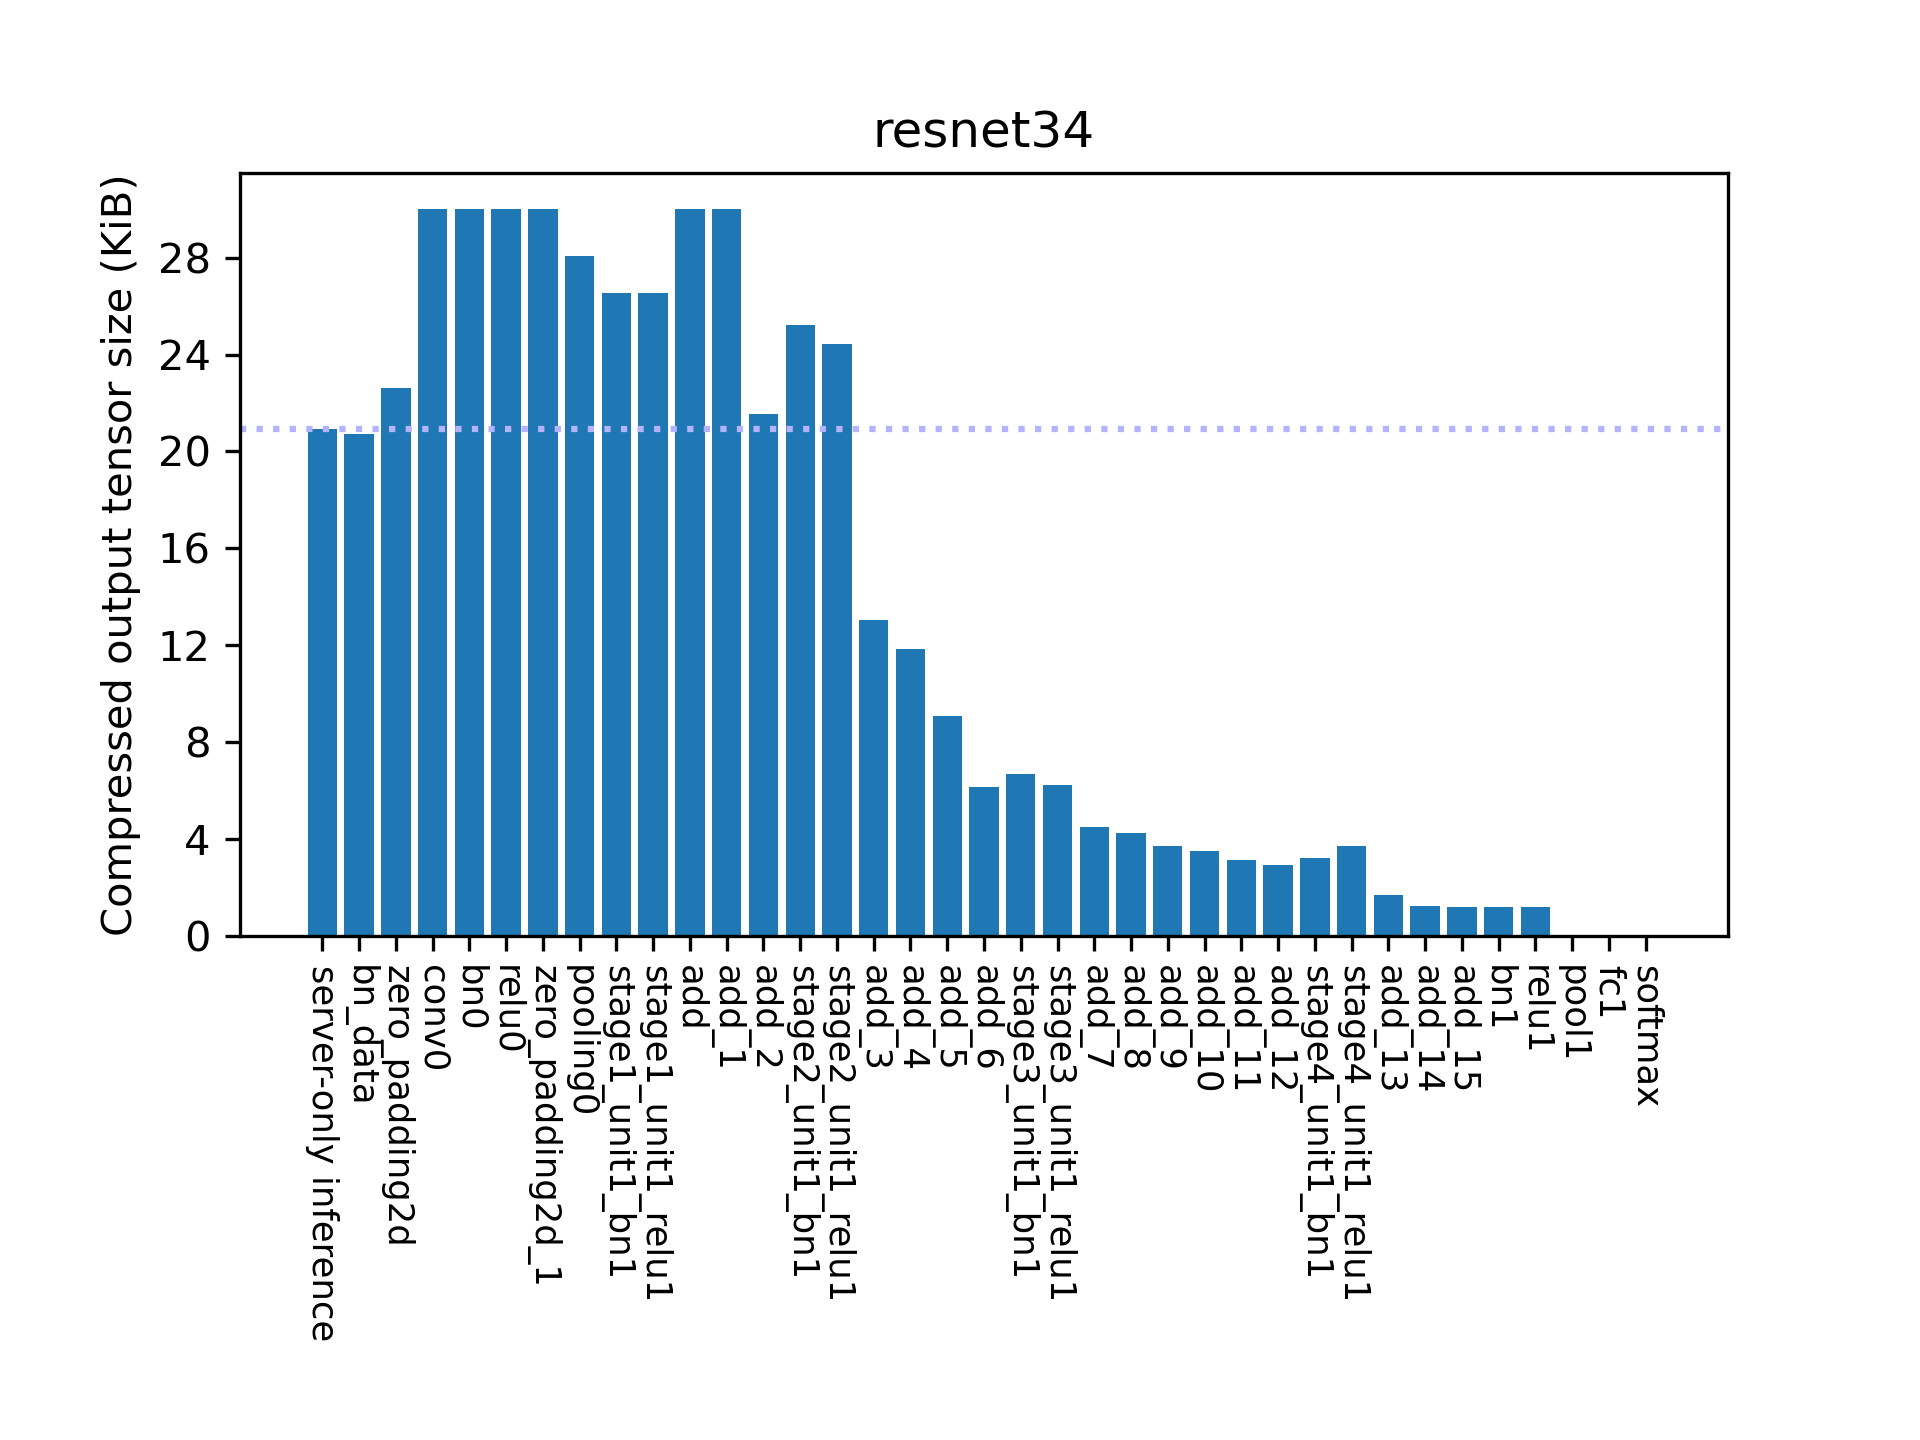
\includegraphics[width=0.8\linewidth]{img/sample.png}
  \caption[Short caption for table of contents goes here.]{%
    Long caption goes here.%
  }
  \label{fig:sample_figure}
\end{figure}


Object detection is a computer vision task that can recognizes the object instances from the digital images. Specifically, the object detection task detects the different classes of object such as person, cup, clock, etc. Understanding object detection allows us to achieve various applications such as “smart vehicle” by which means the system informs the driver if he or she is running in a right direction at a proper speed or system to detect pedestrians in order to prevent the accidents utilizing real-time object detections \cite{gavrila_real-time_1999}. Object detection task can further be developed to object tracking, which is another computer vision task derived from object detection. Object detection task is able to detect the objects for different class type but this task alone has no unique identification of objects within the same class in a sequence of image frames. For example, the system can detect multiple persons but there is no identifications of each person across the frames, and hence object tracking task will assign each unique ID to each object instance.

Video compression is ubiquitous in most of the visual processing pipelines. Compression in video is necessary because without compression of the video, it would be impractical to transmit the video and save in the storage device. For example, 720x480 pixels of full-color 90 min video with 30 frames per second (fps) has 167.96 GB from the group of \citeauthor{ponlatha_comparison_2013} \cite{ponlatha_comparison_2013} is too huge in size to transmit. Since video compression is ubiquitous, any video we access are all pre-compressed and this raises the question of how much the video compression impacts on the object tracking performance. To our knowledge, effects of video compression on object tracking has not been studied well, so the goal of this project is to analyze the effect of video compression on the object tracking performance by assessing on the various metrics that are used for the multiple object tracking.

%\cite{zou_object_2019}.


% \clearpage % force new page

% Insert a figure containing a grid of subfigures:

% \begin{figure}[htb]
  \centering
  \begin{subfigure}{.5\linewidth}
    \centering
    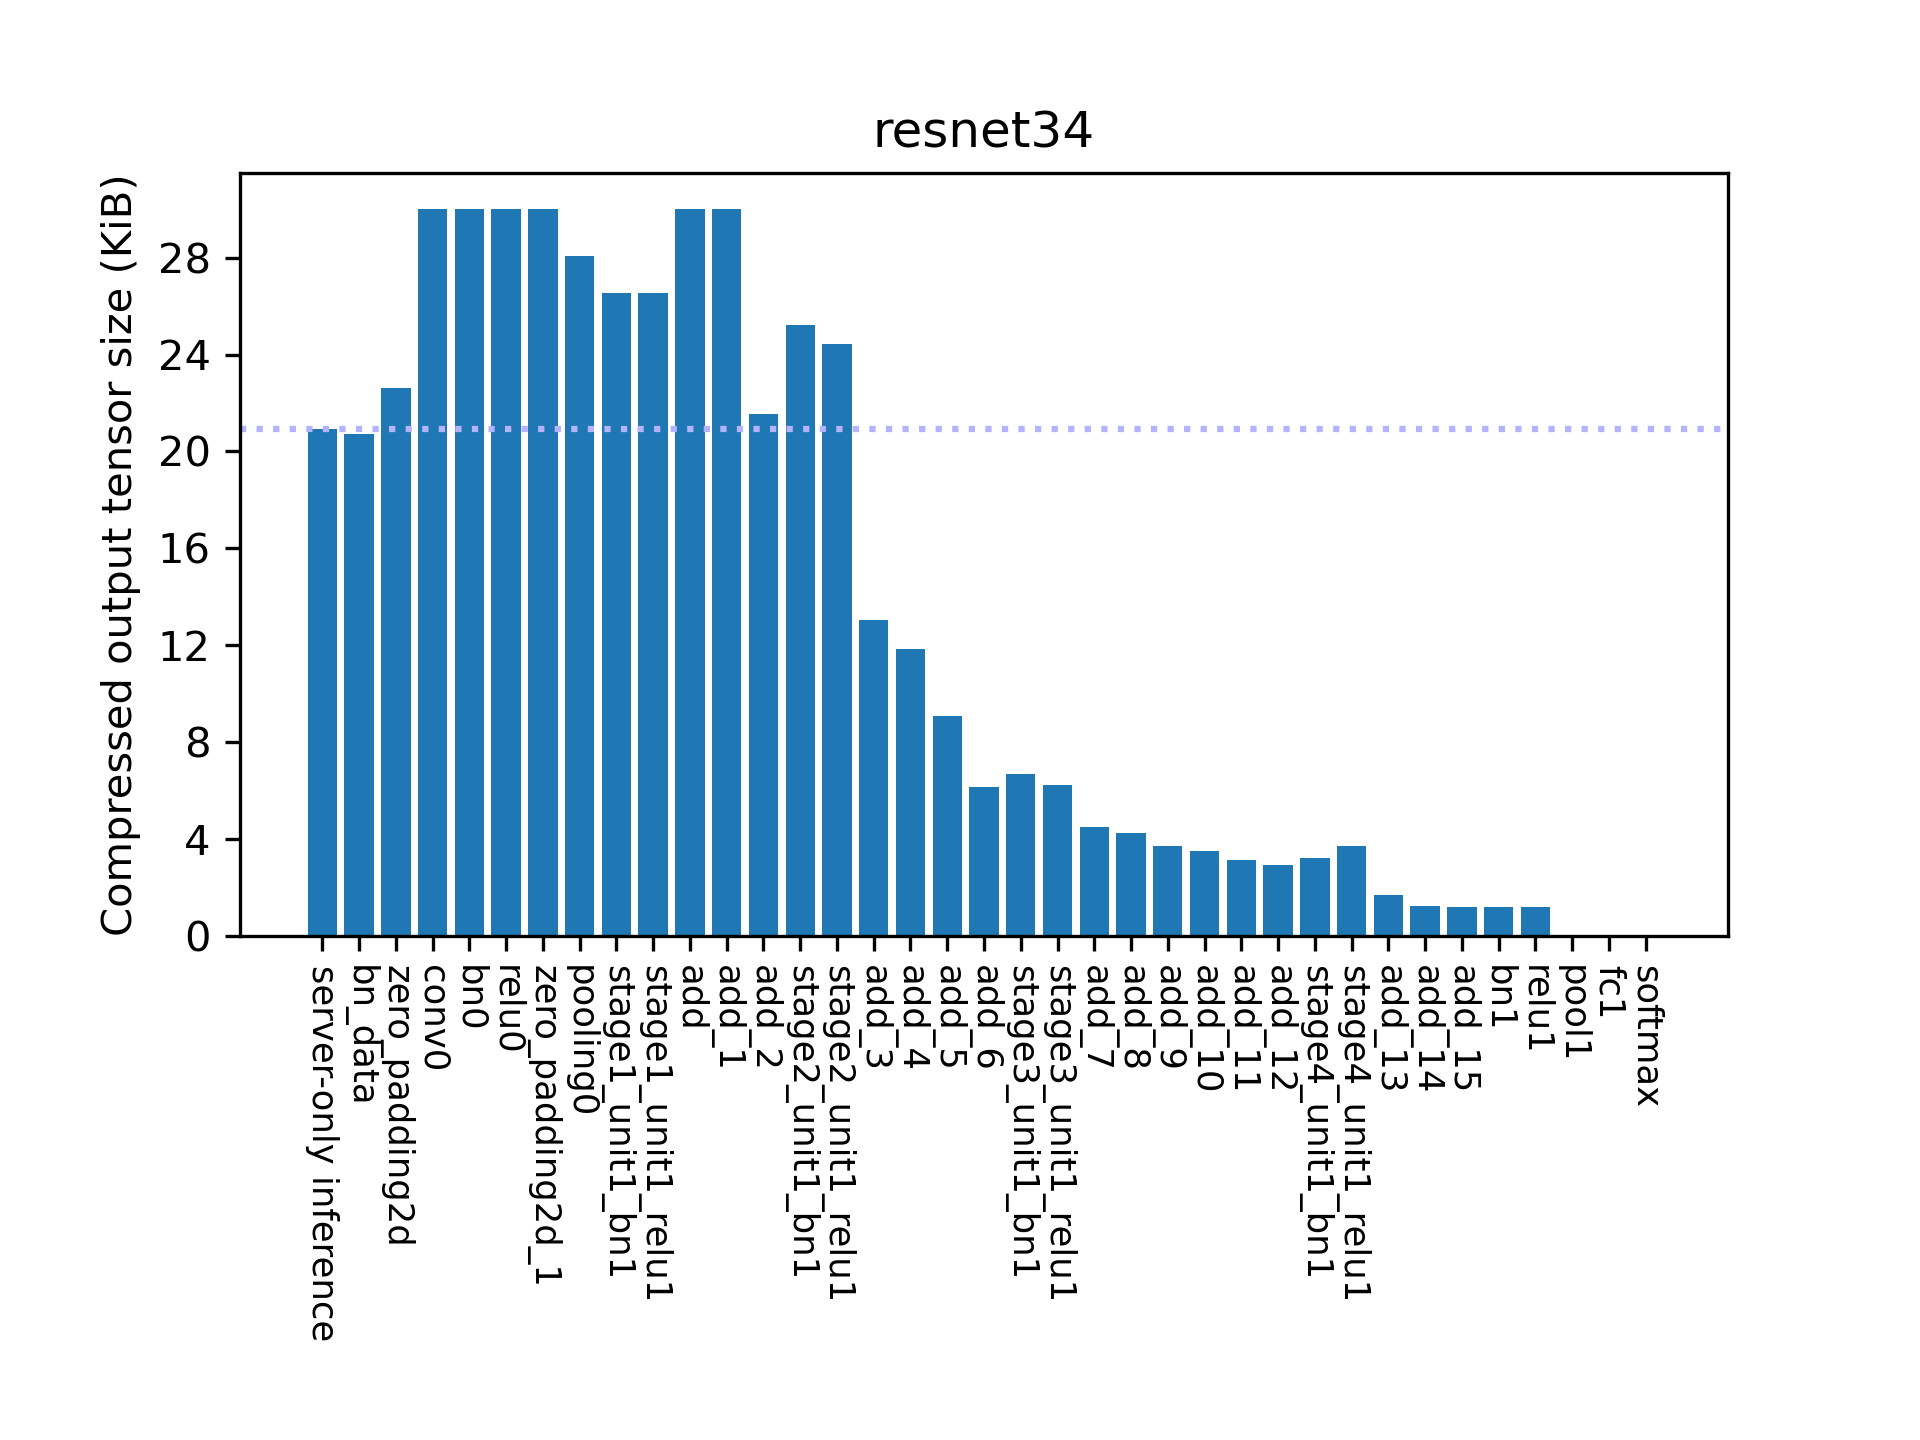
\includegraphics[width=\linewidth]{img/sample.png}
    \caption{top-left}
  \end{subfigure}%
  \begin{subfigure}{.5\linewidth}
    \centering
    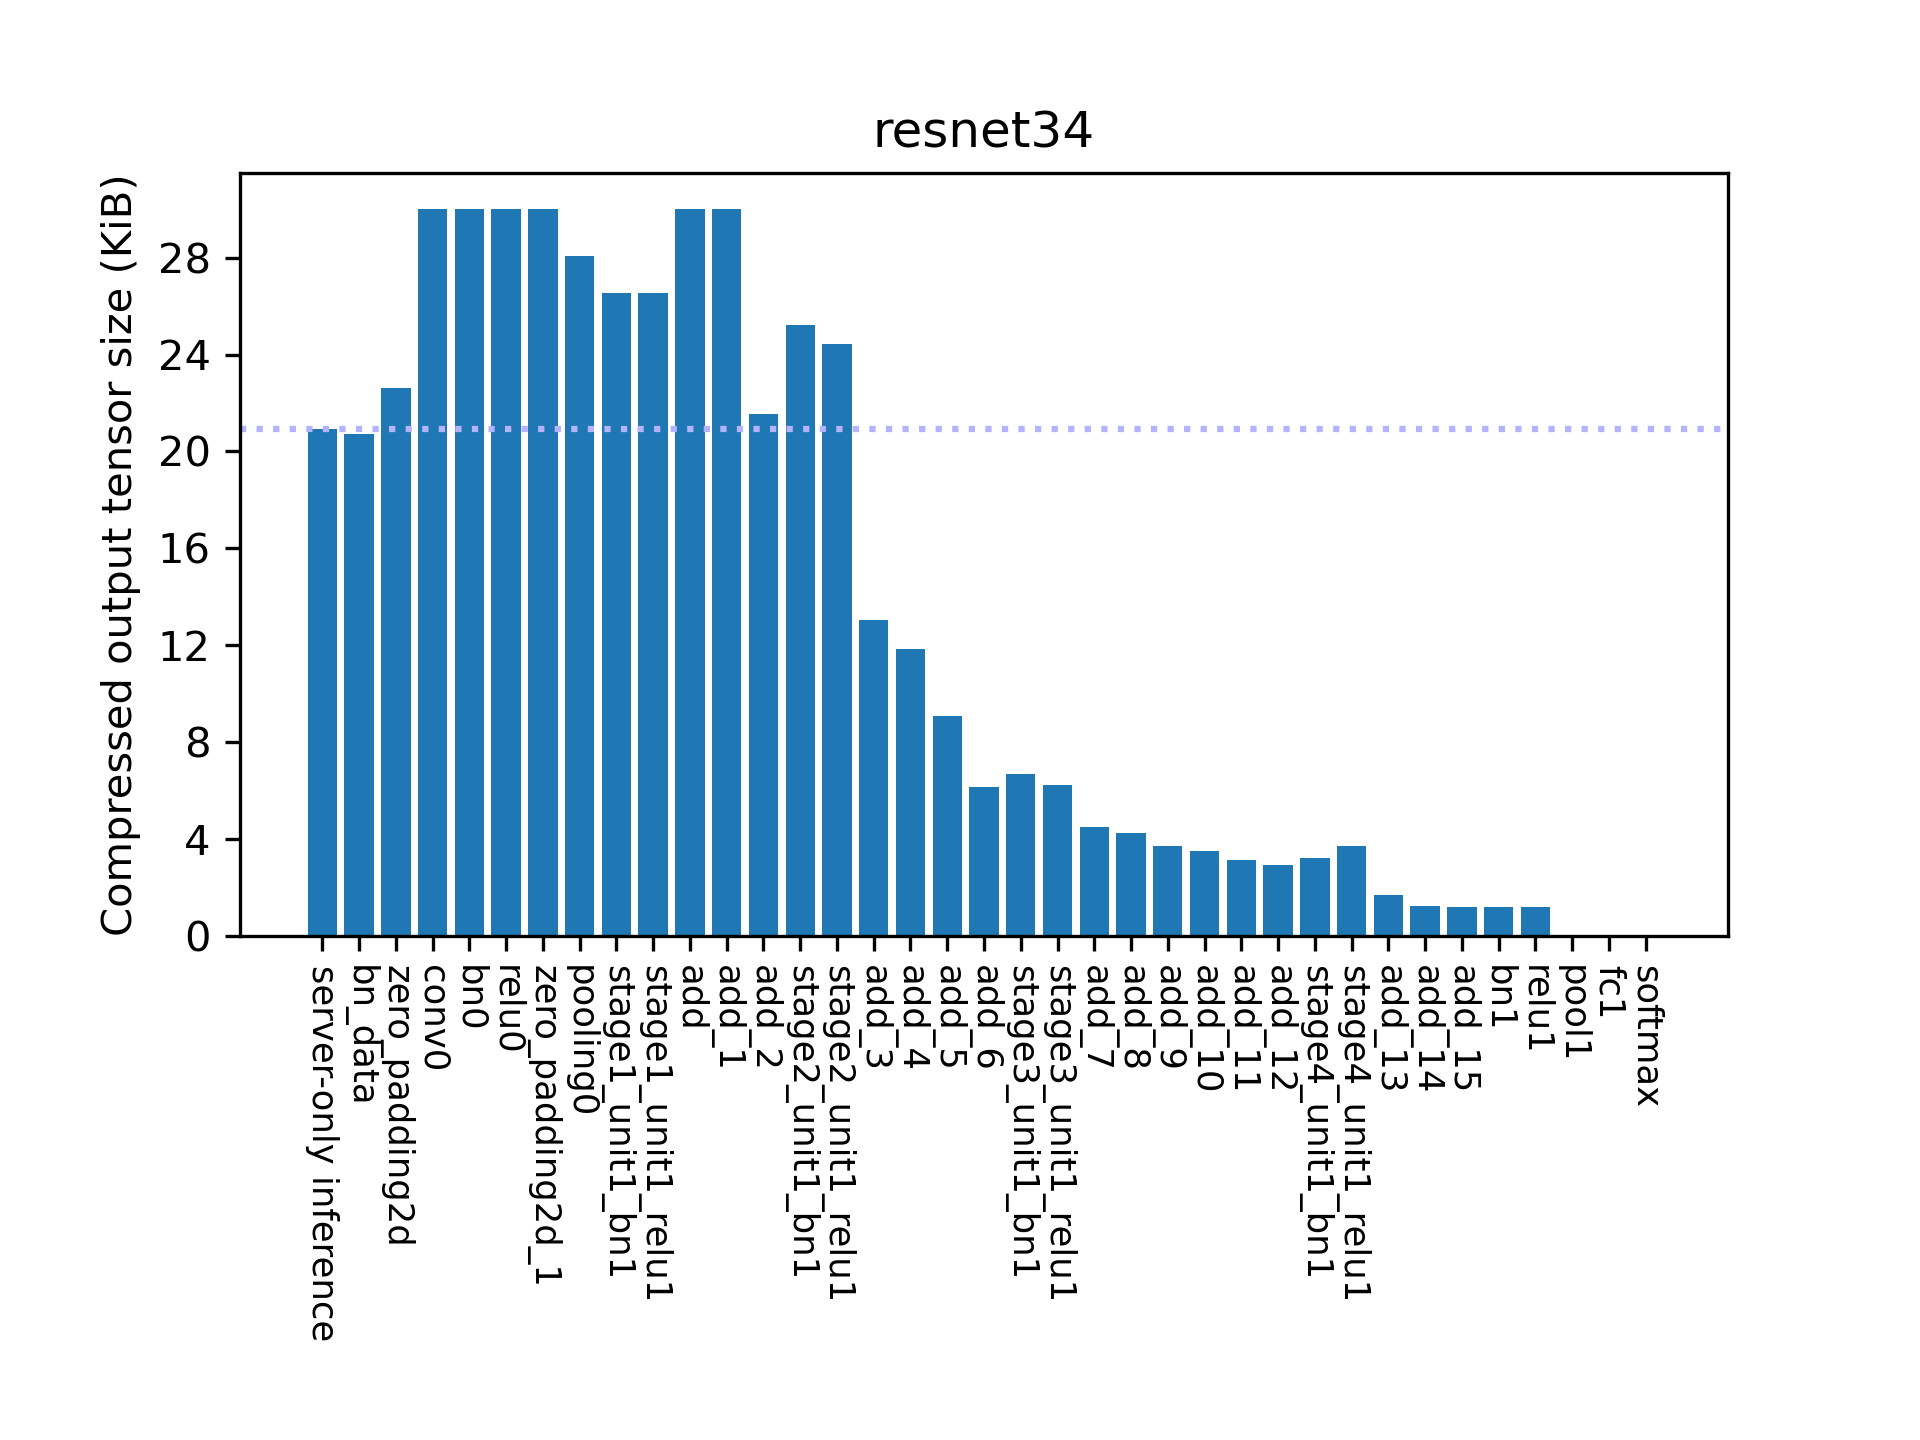
\includegraphics[width=\linewidth]{img/sample.png}
    \caption{top-right}
  \end{subfigure}
  \begin{subfigure}{.5\linewidth}
    \centering
    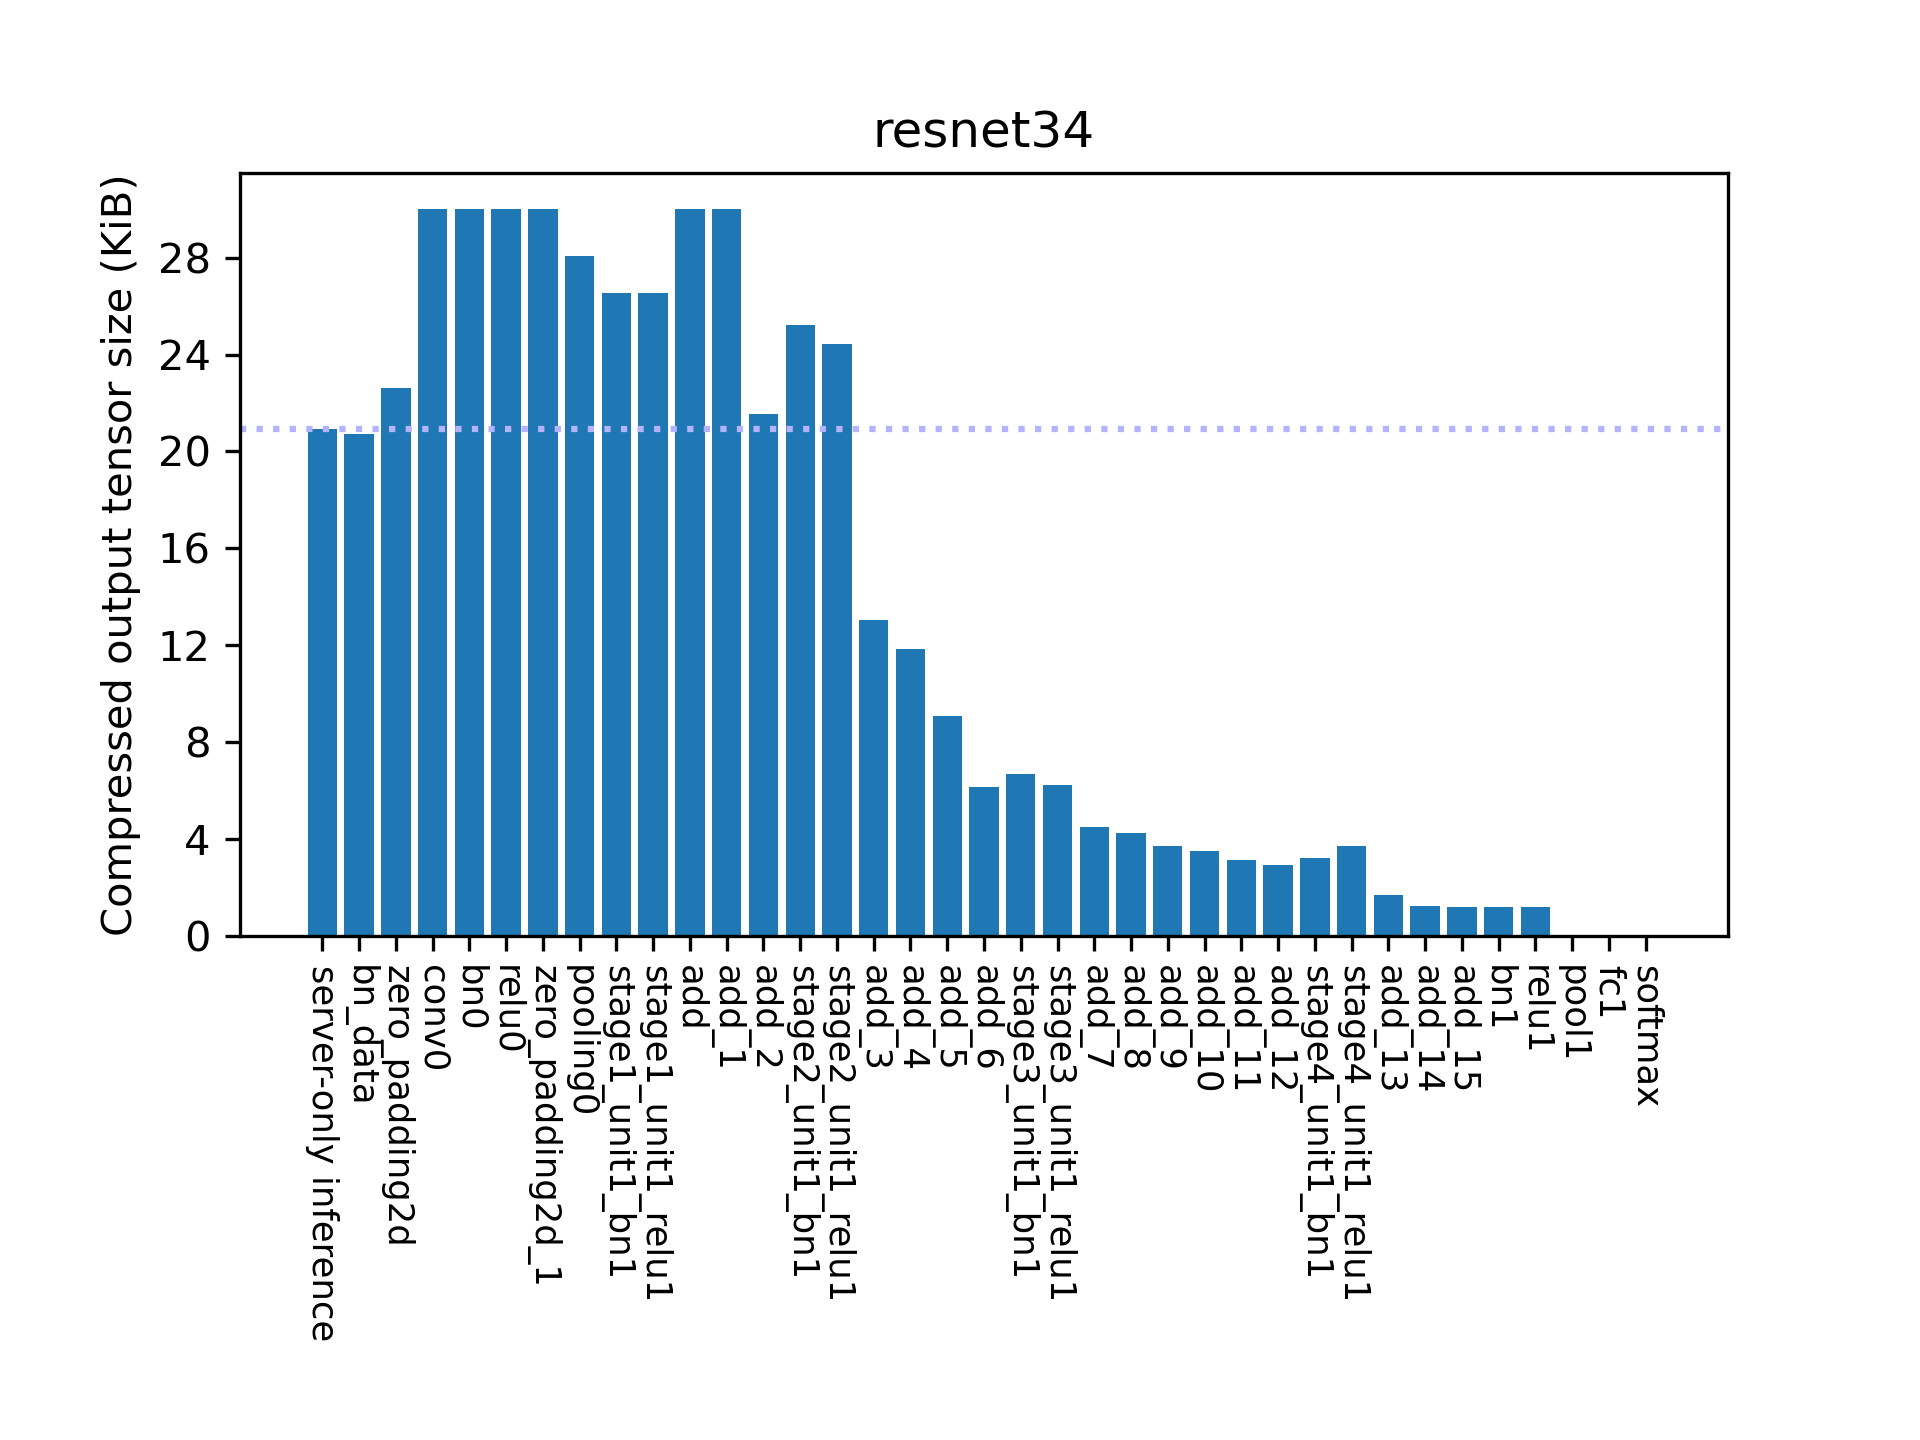
\includegraphics[width=\linewidth]{img/sample.png}
    \caption{bottom-left}
  \end{subfigure}%
  \begin{subfigure}{.5\linewidth}
    \centering
    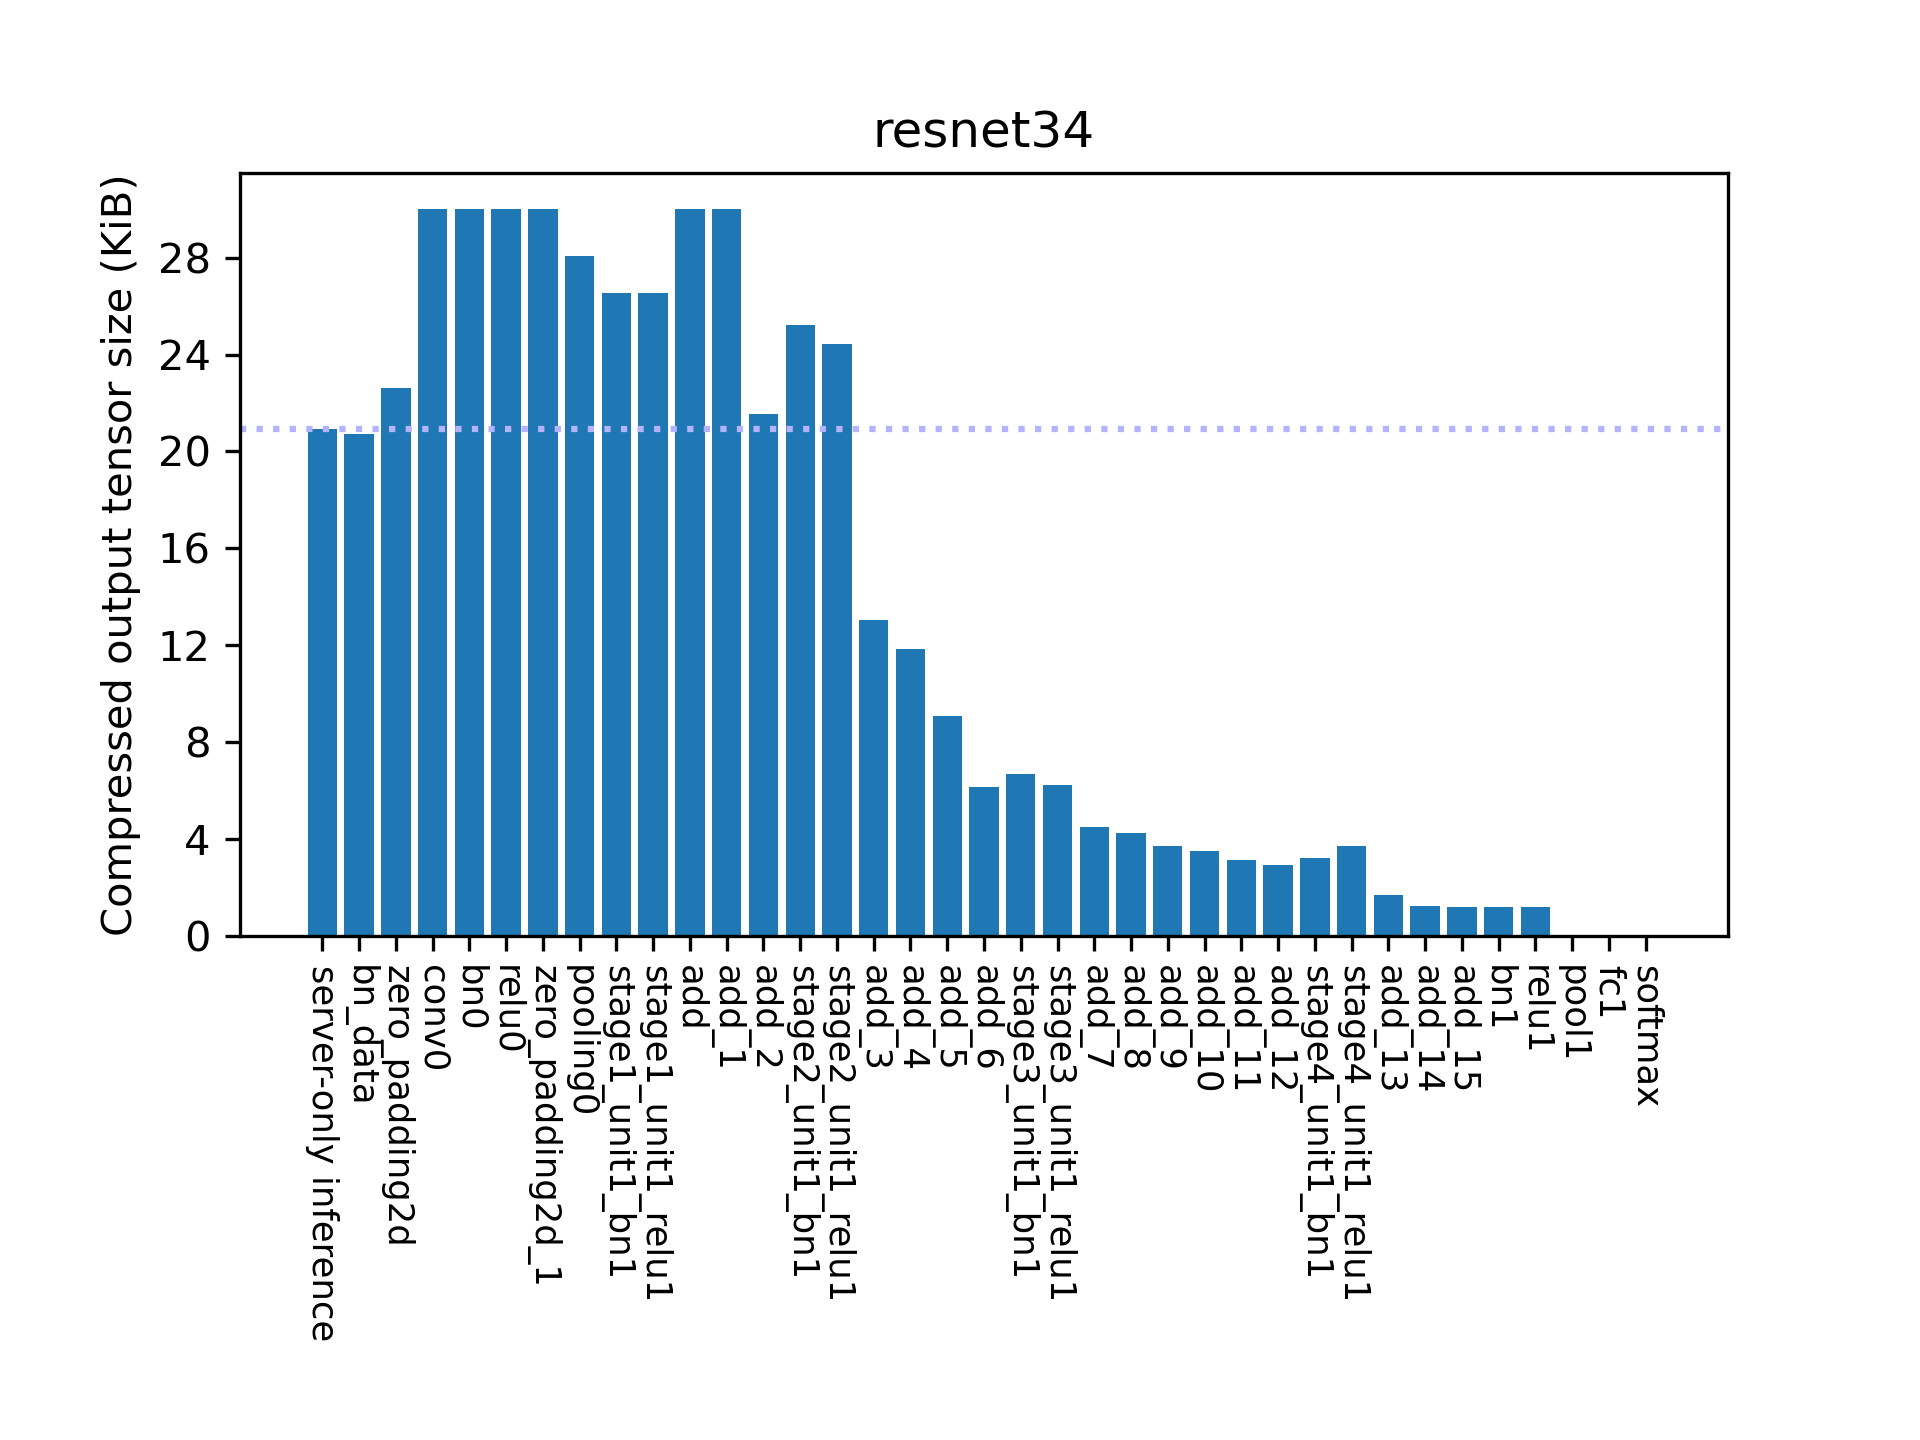
\includegraphics[width=\linewidth]{img/sample.png}
    \caption{bottom-right}
  \end{subfigure}
  \caption[Multiple subfigures example]{%
    A figure containing multiple subfigures. Long caption goes here.%
  }
  \label{fig:sample_figure_grid}
\end{figure}


% % OPTIONAL: \FloatBarrier can be used to prevent figures from floating too far.
% % Use this sparingly! Preferably only when you are doing a final revision.
% \FloatBarrier

% To cite a paper, you can do this~\cite{ioffe2015batch}.
% To reference a figure, chapter, or section within your thesis, try
% \cref{fig:sample_figure} or
% \cref{chap:background} or
% \cref{sec:methods/section_a}.

% If you want to include sections within the chapter,
% I recommend splitting them up into separate files,
% and then using the "input" command to include them.
% If you use Overleaf,
% you can double click on any text in the PDF to jump to its latex code.

% Here are a couple of sections:

\section{Your first section}
\label{sec:introduction/section_a}

Lorem ipsum.


\section{Video Compression}
\label{sec:introduction/section_b}

The early video compression form is first described by Ray Davis Kell in 1929 as the difficulty of transmitting the whole successive images of video can be avoided by only sending the difference between the successive images, though it was not actually used however became the foundation for the video compression standards today \cite{jacobs_brief_2009}. \citeauthor{jacobs_brief_2009} explained that the video system was originated from the oscilloscope with Cathode Ray Tubes. The early video compression was the analog system but the digital video processing has been developed and is widely used today. \citeauthor{zhang_overview_2019} explained the concept of typical video compression today as following \cite{zhang_overview_2019}. The video compression consists of the encoder to compress the images into the compressed form which can be stored or transmits to the other location, and decoder to de-compress the images. This process of coding and de-coding is also called codec. The typical video compression standards nowadays comprise of predictive coding, transform coding, and entropy coding as shown in Fig. \ref{fig:comp_architecture}. Predictive coding is the component that reduces the inter-frame temporal redundancy and intra-frame spatial redundancies of video by motion estimation (ME) and motion compensation (MC) techniques. Transform coding is the component where the transform coefficients that are quantized are generated through discrete cosine transforms (DCT) to help reducing the spatial dependencies. Entropy coding is the component where compressed bit streams are generated.

\begin{figure}[!tb]
  \centering
  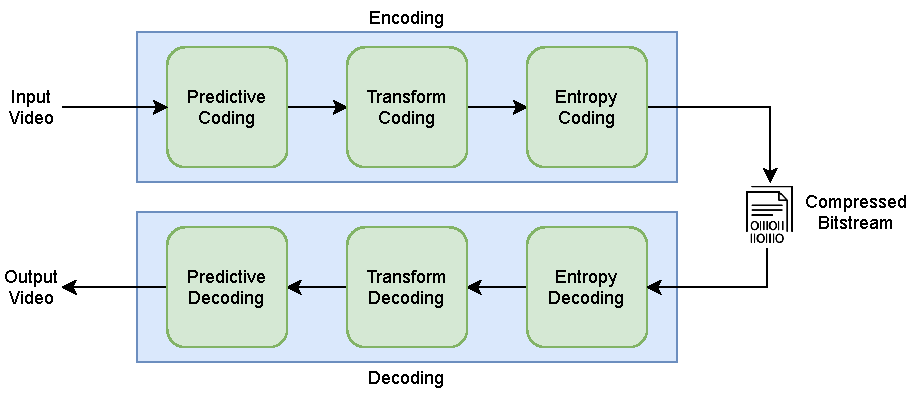
\includegraphics[width=0.8\linewidth]{img/comp_architecture.pdf}
  \caption[The typical video compression architecture]
  {
  The typical video compression architecture adapted from \cite{zhang_overview_2019}.
%   The encoder consists of predictive coding, transform coding, and entropy coding compresses the input video and generates the compressed bitstream. The decoder decompresses the bitstream in reverse order to the encoder and outputs the reconstructed video.
  }
  \label{fig:comp_architecture}
\end{figure}

There are two type of video coding; losssless coding and lossy coding. Lossless coding compresses the images and reconstructed images can be obtained after de-compression without any loss of information. Lossy coding however compresses the images by removing the less important information, which will sacrifice the image quality to the level the human visual system can be tolerant. Lossy compression is more widely used today since it allows much lower compressed size and more efficient than the lossless manner.

Since the first video compression standard of H.120 that has been developed in 1984, the various video compression standards have been developed such as MPEG and H.26X series \cite{zhang_overview_2019}.




The organization of Video Coding Expert Group (VCEG) of International Telecommunication Union (ITU-T) are developing H.26X series starting from the first standard of H.120, then developed H.261, H.262, H.263, H.264(AVC), and H.265 (HEVC). H.264 or so called Advanced Video Coding (AVC) were developed in 2003 and the typical architecture shown in Fig.\ref{fig:comp_architecture} were followed since H.264/AVC. H.264/AVC is the most widely used standard nowadays and supports up to 4k (4096×2304) resolution of video.


\section{Thesis preview}
\label{sec:introduction/thesis_preview}

As an organization of this thesis, we start by illustrating Chapter 1 the motivation for this research and providing history and background information for each object tracking and video compression concept. We will then explain the more detailed background information on the adopted methods in Chapter 2. Chapter 3 shows the methodologies and experimental procedures. Chapter 4 illustrates the results from the experiment and data analysis. Finally, we will conclude this research with the highlighted insights and future work in Chapter 5. The additional information is included in Appendix.

\chapter{Background}
\label{chap:background}

A short preview of this chapter.


\section{YOLOv3 Object Detector}
\label{sec:background/section_a}

% -------------------------------------------------------
% old text, too much information in YOLO, YOLOv2, YOLOv3 % 
% -------------------------------------------------------

\begin{comment}

As one of the deep learning-based and one-stage object detectors whereby the full image itself is applied to the single neural network, You Only Look Once (YOLO) was considered for our object detection component in the object tracking system. The following conceptual background in YOLO was described by \citeauthor{redmon_you_2016} \cite{redmon_you_2016}. YOLO is a convolutional neural network-based model, and it divides the input image into $S \times S$ grids. Each cell in the grids is responsible for predicting the dimension of $B$ number of bounding boxes. Each bounding box has a center coordinate of $x, y$ and width, and the height of $w, h$ as a dimension, and Intersection over Union (IOU) can be calculated between the dimension of the predicted bounding box and ground truth bounding box. Each cell also predicts the probability of the object contained by the bounding box and the conditional probability of the object belonging to a specific class given the object contained by the bounding box. Based on these three predictions, YOLO gives the class-specific confidence value as,
\begin{equation}
P(class_i | object) \times P(Object) \times IOU = P(class_i) \times IOU,
\label{eq:yolo_conf}
\end{equation}
which is given by \citeauthor{redmon_you_2016}. The dimension of final prediction tensor will be $S \times S \times (B \times 5 + C)$ where $C$ is the number of classes we want to detect and the value 5 contains $x$, $y$, $w$, $h$, and the class-specific confidence score.

YOLO is much faster in speed and suitable to the real-time application but gives relatively lower accuracy than other state-of-the-art two-stage object detectors and hard to localize the small objects. Also, as a limitation, each cell in the grid can predict 2 boxes ($B=2$) but only estimate one class. YOLOv2 has been developed to resolve some issues that exist in YOLO as well as incremental improvements as described by \citeauthor{redmon_yolo9000_2017} \cite{redmon_yolo9000_2017}. YOLOv2 primarily focuses on improving recall and localization while preserving classification errors and speed. Anchor boxes have been implemented to predict the bounding boxes based on the chosen anchor boxes. Using anchor boxes, YOLOv2 estimates a bounding box by an offset from the anchor box instead of estimating the coordinates directly as in YOLO. This allows the network to learn easier and detect multiple objects per cell from multiple anchor boxes. The anchor boxes have been automatically chosen using k-means clustering. Other features are also implemented in YOLOv2, such as batch normalization, high-resolution classifier, and multi-scale training, providing better speed and accuracy. YOLOv3 has been developed as an incremental improvement to the YOLOv2 as described by \citeauthor{redmon_yolov3_2018} \cite{redmon_yolov3_2018}. Similar to YOLOv2, YOLOv3 predicts bounding boxes based on anchor boxes with k-means clustering, and the logistic regression has been implemented to predict the objectiveness score. If the bounding box overlaps on the ground truth more than any other anchor boxes, the objectiveness score will be 1. However, other bounding boxes will be ignored in this cell if they overlap more than than the defined IOU threshold. As other improvements, YOLOv3 uses an independent logistic classifier instead of softmax that is implemented in YOLOv2 to allow multi-label class predictions. Also, YOLOv3 predicts tensor at 3 different scales across the network, and the dimension of the final encoded tensor will be $S \times S \times k \times (5 + C)$ where $k$ is the number of anchor boxes. With these improvements, YOLOv3 achieves localizing smaller objects while maintaining speed and accuracy.

\end{comment}


% -------------------------------------------------------
% re-write here % 
% -------------------------------------------------------

You Only Look Once (YOLO) \cite{redmon_you_2016} was selected for our object detection component in the object tracking system. The following conceptual background of YOLO was described by \citeauthor{redmon_you_2016} \cite{redmon_you_2016}. YOLO is a convolutional neural network-based model, and it divides the input image into $S \times S$ grids. Each cell in the grid predicts the bounding box information and the object class probability. YOLO is much faster in speed and more suitable for real-time applications but gives somewhat lower accuracy than other state-of-the-art object detectors. YOLOv2 \cite{redmon_yolo9000_2017} has been developed as an improvement to its predecessor YOLO. YOLOv2 primarily focuses on improving recall and localization while preserving classification accuracy and speed. Anchor boxes have been implemented to improve recall, and YOLOv2 with anchor boxes can predict a lot more bounding boxes than YOLO. YOLOv2 estimates a bounding box by an offset from a candidate anchor box instead of estimating the coordinates directly as in the original YOLO. As an incremental improvement to YOLOv2, YOLOv3 \cite{redmon_yolov3_2018} has been developed. The highlighted improvements are as follows; the logistic regression has been implemented to predict the objectness score. If the bounding box overlaps the ground truth more than any other anchor boxes, the objectness score will be 1. YOLOv3 uses an independent logistic classifier instead of softmax implemented in YOLOv2 to allow multi-label class predictions. Finally, YOLOv3 predicts bounding boxes and the corresponding object classes at 3 different scales across the network, similar to Feature Pyramid Network \cite{lin_feature_2017}. With these improvements, YOLOv3 achieves localization of smaller objects while maintaining speed and accuracy.

We have chosen the YOLOv3 object detector developed by Ultralytics \cite{jocher_ultralyticsyolov3_2021} with the provided pre-trained weights. The developer \citeauthor{jocher_ultralyticsyolov3_2021} pre-trained the network with the backbone of Darknet53, and the model has 261 layers with 61,922,845 parameters. The COCO dataset was used for training with 118,287 training images, 5,000 validation images, and 20,288 out of 40,670 test images. This network with the pre-trained weights can detect up to 80 object classes available from the COCO dataset \cite{lin_microsoft_2014}. To compare the chosen YOLOv3 detector from Ultralytics with the original implementation of YOLOv3 by \citeauthor{redmon_yolov3_2018}, the comparison of Mean Average Precision (mAP) on the COCO dataset has been shown in Table \ref{tab:yolov3_comparison}. The mAP value from the original implementation of Darknet53 is reported by the author \citeauthor{redmon_yolov3_2018}, and the value from the Ultralytics implementation is reported by \citeauthor{jocher_ultralyticsyolov3_2021} \cite{jocher_ultralyticsyolov3_2021}. mAP is a detection performance metric, and it averages Average Precision (AP) values from different object classes. In the COCO Detection Challenge, mAP also averages AP values at 10 intersection over union (IOU) thresholds from 0.5 to 0.95 \cite{lin_microsoft_2014} \cite{noauthor_coco_nodate}. mAP-50 is a detection performance metric at IOU threshold of 0.5 in particular, and its detail definition is explained in Chapter \ref{sec:background/section_d}. The mAP and mAP-50 are reported based on Microsoft COCO dataset. As Table \ref{tab:yolov3_comparison} shows, our chosen detector from Ultralytics achieves better detection performance than the original implementation of Darknet53.
\begin{table}[!tb]
    \centering
    \caption[Comparison of YOLOv3 software with the original implementation]
    {Comparison of YOLOv3 software with the original implementation.}
     \begin{tabular}{||c | c | c c||} 
     \hline
      - & Resolution & mAP & mAP-50 \\ [0.5ex]
     \hline\hline
      YOLOv3, Darknet53 & 608x608 & 33.0 & 57.9\\ 
     \hline
     YOLOv3, Ultralytics & 640x640 & 43.3 & 63.0 \\
     \hline
    \end{tabular}
    \label{tab:yolov3_comparison}
\end{table}

\section{Simple Online Realtime Tracking (SORT)}
\label{sec:background/section_b}

The detection-based tracking requires an object detector to initialize the tracker's state by detecting the objects, then a tracking component will track those objects. Multiple object tracking problem can be viewed as a data association problem in assigning the optimal unique identity to each object. Simple Online Realtime Tracking (SORT) was selected for the tracking component, which is a detection-based online tracker with a deterministic output. As \citeauthor{bewley_simple_2016} describe \cite{bewley_simple_2016}, based on the detected objects, SORT utilizes the constant linear motion model to estimate the displacements of the objects across the frames. The tracker's state at time $k$ can be represented as a state vector:
\begin{equation}
\mathbf{x}_{k} = [u, v, s, r, \dot{u}, \dot{v}, \dot{s}]^\mathsf{T}~,
\label{eqn:state_vector}
\end{equation}
where $u$ and $v$ are the pixel coordinates in the horizontal and vertical direction; $s$ and $r$ are the area and aspect ratio of the bounding box; $\dot{u}$ and $\dot{v}$ represent the velocity; $\dot{s}$ is the rate of change of the area. The aspect ratio $r$ is assumed to be constant, and hence the state vector does not include $\dot{r}$. SORT utilizes the Kalman filter \cite{kalman_new_1960} (the original publication by \citeauthor{kalman_new_1960}) to estimate the state vector optimally. The use of Kalman filter in the multiple object tracking is explained well by \cite{li_multiple_2010} and adapted from this explanation, we described the framework as following. Also, we adapted the following equations according to the source code of SORT \cite{abewley_abewleysort_2021} and the library source code of the Kalman filter \cite{labbe_rlabbefilterpy_2021}.

Kalman filter framework can be implemented recursively to estimate the object's state in the next frame based on the previous state as well as its error. Recall that we utilizes YOLOv3 for object detection, so the measurements, detected bounding boxes in our case, are taken at every frame. The measurement vector can be represented as
\begin{equation}
\mathbf{z}_{k} = [u, v, s, r]^\mathsf{T}
\label{eqn:measurement_vector}
\end{equation}
The Kalman filter framework allows us to estimate the apriori state vector $\mathbf{\hat{x}}^-$ and apriori covariance matrix $\mathbf{P}^-$ at time $k$ based on the previous state and covariance at time $k-1$.
\begin{equation}
\mathbf{\hat{x}}_{k}^{-} = \mathbf{A} \mathbf{\hat{x}}_{k-1} ~ ,
\label{eqn:state_apriori_update}
\end{equation}
\begin{equation}
\mathbf{P}_{k}^- = \mathbf{A}\mathbf{P}_{k-1}\mathbf{A}^\mathsf{T}+\mathbf{Q}
\label{eqn:error_apriori_update}
\end{equation}
$\mathbf{A}$ is a transition matrix represented as
\begin{equation}
\mathbf{A} = \left[ \begin{matrix} 1 & 0 & 0 & 0 & 1 & 0 & 0 \\ 0 & 1 & 0 & 0 & 0 & 1 & 0 \\ 0 & 0 & 1 & 0 & 0 & 0 & 1 \\ 0 & 0 & 0 & 1 & 0 & 0 & 0 \\ 0 & 0 & 0 & 0 & 1 & 0 & 0 \\ 0 & 0 & 0 & 0 & 0 & 1 & 0 \\ 0 & 0 & 0 & 0 & 0 & 0 & 1 \end{matrix} \right]
\label{eqn:transition_matrix}
\end{equation}
The measurement vector at time $k$ can be obtained from the state vector $\mathbf{x}_k$ as
\begin{equation}
\mathbf{z}_{k} = \mathbf{H} \mathbf{x}_{k} ~ ,
\label{eqn:measurement_eqn}
\end{equation}
where $\mathbf{H}$ is a measurement matrix represented as
\begin{equation}
\mathbf{H} = \left[ \begin{matrix} 1 & 0 & 0 & 0 & 0 & 0 & 0 \\ 0 & 1 & 0 & 0 & 0 & 0 & 0 \\ 0 & 0 & 1 & 0 & 0 & 0 & 0 \\ 0 & 0 & 0 & 1 & 0 & 0 & 0 \end{matrix} \right]
\label{eqn:measurement_matrix}
\end{equation}
Given the apriori estimates from Equation \eqref{eqn:state_apriori_update}, \eqref{eqn:error_apriori_update} and the estimated measurement $\mathbf{H} \mathbf{\hat{x}}_{k}^-$, Kalman filter framework corrects the apriori estimates, updating them to have aposteriori estimates using the current measurement $\mathbf{z}_k$. The equations for the aposteriori estimates will be
\begin{equation}
\mathbf{K}_{k} = \mathbf{P}_{k}^{-} \mathbf{H}^\mathsf{T} (\mathbf{H} \mathbf{P}_{k}^{-} \mathbf{H}^\mathsf{T} + \mathbf{R} )^{-1} ~ ,
\label{eqn:Kalman_gain_update}
\end{equation}
\begin{equation}
\mathbf{\hat{x}}_{k} = \mathbf{\hat{x}}_{k}^- + \mathbf{K}_{k} (\mathbf{z}_k - \mathbf{H} \mathbf{\hat{x}}_{k}^-) ~ ,
\label{eqn:state_aposteriori_estimate}
\end{equation}
\begin{equation}
\mathbf{P}_k = (1 - \mathbf{K}_k \mathbf{H} ) \mathbf{\hat{P}}_k^- ~ ,
\label{eqn:error_aposteriori_estimate}
\end{equation}
where $\mathbf{K}_{k}$ is the Kalman gain at time $k$. The Kalman gain $\mathbf{K}_k$, the aposteriori estimate of state vector $\mathbf{x}_k$, and the aposteriori estimate of error covariance matrix $\mathbf{P}_k$ are recursively updated by the estimated apriori state vector $\mathbf{\hat{x}}_{k}^{-}$ and apriori error covariance matrix $\mathbf{P}_{k}^{-}$. Therefore, the Kalman filter framework essentially consists of the prediction steps that will estimate the bounding boxes as apriori estimates and the correction steps that will correct the predicted information as aposteriori estimates, and the process will be recursively back to the prediction steps to proceed with the next frame. For the initial conditions, when the object is detected, the velocity components are set to 0 for the state vector $\mathbf{x}_0$.
\begin{equation}
\mathbf{x}_{0} = [u, v, s, r, 0, 0, 0]^\mathsf{T}
\label{eqn:x_0}
\end{equation}
For the covariance matrix $\mathbf{P}_0$, the velocity components are set to large variance values as $10^4$ since no velocity is observed at the initial state.
\begin{equation}
\mathbf{P}_0 = \left[ \begin{matrix}   
  10  &  0  &  0  &  0  &  0  &  0  &  0 \\
  0  &  10  &  0  &  0  &  0  &  0  &  0 \\
  0  &  0  &  10  &  0  &  0  &  0  &  0 \\
  0  &  0  &  0  &  10  &  0  &  0  &  0 \\
  0  &  0  &  0  &  0  &  10^4  &  0  &  0 \\
  0  &  0  &  0  &  0  &  0  &  10^4  &  0 \\
  0  &  0  &  0  &  0  &  0  &  0  &  10^4 
  \end{matrix} \right]
\label{eqn:P_0}
\end{equation}
For the process noise covariance $\mathbf{Q}$ and the measurement noise covariance $\mathbf{R}$, constant values are assigned.
\begin{equation}
\mathbf{Q} = \left[ \begin{matrix} 
1 & 0 & 0 & 0 & 0 & 0 & 0 \\ 
0 & 1 & 0 & 0 & 0 & 0 & 0 \\ 
0 & 0 & 1 & 0 & 0 & 0 & 0 \\ 
0 & 0 & 0 & 1 & 0 & 0 & 0 \\ 
0 & 0 & 0 & 0 & 10^{-2} & 0 & 0 \\
0 & 0 & 0 & 0 & 0 & 10^{-2} & 0 \\ 
0 & 0 & 0 & 0 & 0 & 0 & 10^{-4} \end{matrix} \right]
\label{eqn:P_0}
\end{equation}
\begin{equation}
\mathbf{R} = \left[ \begin{matrix}   
  1  &  0  &  0  &  0 \\
  0  &  1  &  0  &  0 \\
  0  &  0  &  10 &  0 \\
  0  &  0  &  0  &  10 \end{matrix} \right]
\label{eqn:R}
\end{equation}
These initial conditions and noise matrices used the default values by \cite{bewley_simple_2016}.

As for the data association, the assignment cost matrix, consisting of IOU values between each measured bounding box and predicted box by the Kalman filter, can be computed. The assignments of unique identities on a current frame can be solved optimally from this matrix via the Hungarian algorithm \cite{kuhn_hungarian_1955}. When the measured object overlaps less than the minimum IOU threshold value with the predicted bounding box, the assignment for the measured bounding box will be rejected. For the trajectories initialization, however, the untracked objects are found when the detected objects overlap less than the minimum IOU threshold with the predicted bounding boxes. Followed by the minimum number of detections, the trajectories with the unique identities are initialized. When the objects are not detected for a certain number of frames labeled as $T\textsubscript{Lost}$, the trajectories are terminated.

SORT is focused on simplicity of design, which could serve as a baseline tracking method. This is because SORT essentially consists of a Kalman filter framework for predicting motion and a Hungarian algorithm for data association. However, it does not deal with long-term occlusions. Adding the object re-identification feature to deal with occlusions will weigh significant complexities on the tracker. SORT is simple yet fast, and maintains high accuracy with deterministic output. Combined with a fast YOLOv3 object detector, SORT will make it easy for us to run the experiments since both components are fast enough and produce deterministic results.

\section{High Efficiency Video Coding (HEVC)}
\label{sec:background/section_c}

H.265/HEVC is the video compression standard developed by ITU-T Video Coding Expert Group in 2013. H.265/HEVC follows the same structure of its predecessor H.264/AVC as shown in the Fig.\ref{fig:comp_architecture} but achieves a better coding performance. The typical structure consists of predictive coding with intra-frame and inter-frame prediction, transform coding that generates the quantized transform coefficients from DCT, and finally the entropy coding that generates a compressed bitstream. To obtain the de-compressed video, HEVC performs entropy decoding, transform decoding, and predictive decoding, which is in a reversed order to the encoding part \cite{zhang_overview_2019}. For the experiment, we have used the lossy compression of HEVC test model (HM) at version 16.20, and selected two parameters of compresson settings varied for the experiment; quantization parameter and motion search range.

\subsection{Quantization Parameter}
Quantization parameter (QP) is the parameter used in the transform coding. The value of QP determines the quantization step size by which we obtain the quantized transform matrix. QP ranges from 0 to 51 and an increase of 6 in QP will double the quantization step size \cite{sullivan_overview_2012} \cite{budagavi_hevc_2014}. According to \cite{sharrab_modeling_2017}, QP has a significant impact on bitrate. They showed that bitrate is inversely proportional to QP and the pixel rate is linear proportional to the pixel rate. This means that high QP will result in lower bitrate and hence lower pixel rate. In other words, high QP will cause resolution to be lower while low QP will sustain high resolution.

\subsection{Motion Search Range}
Motion estimation is inter-frame prediction technique that finds the best match of the block of regions between the previous reference frame and the current frame while minimizing the rate-distortion cost or highest correlation. Motion estimation is essentially reducing the temporal redundancies by obtaining a motion vector that points from the region in the previous reference frame toward the target candidate region in the current frame. This block of region is search window and its size is considered as search range (SR). The high SR value uses a larger search window and hence requires more memory in bandwidth but low SR uses a smaller search window and requires less memory  \cite{lou_adaptive_2010} \cite{bachu_review_2015}. From this logic, we can interpret that the large search window could cover fast motion in a video with SR high enough, while the low SR only covers the slower motion. In the experiment, we label the parameter as motion search range (MSR).



\section{Multiple Object Tracking Metrics}
\label{sec:background/section_d}

To evaluate the object detection and tracking performance quantitatively, we need metrics to quantify the performance with respect to the ground truth. Since there is no single metric that captures all aspects of the tracking performance, various metrics have been considered as listed below. The arrow symbol $\uparrow$ indicates "the higher, the better", while $\downarrow$ indicates "the lower, the better". We utilized the software from \cite{heindl_cheindpy-motmetrics_2021} to evaluate the performance metrics.

\subsection{Detection Performance Measure}
The following metrics of TP, FP, FN, Precision, Recall, F1, and mAP-50 measure the detection performance. TP, FP, and FN are based on the value of Intersection over Union (IOU) threshold, which is defined as the area of intersection of the detected bounding box and the ground truth bounding box, divided by the union of those boxes. For example, if we set the IOU threshold to 0.5 and obtain the IOU value of 0.8 at the target object, we count it as TP. If we obtain the IOU value of 0.2, we then count it as FP. If there is no detected bounding at the ground truth target, FN will be counted. The following definitions of detection performance measure are explained in \cite{ristani_performance_2016} \cite{milan_mot16_2016}. For mAP-50, we explained the definition adapted from \cite{padilla_survey_2020} and \cite{padilla_comparative_2021}.

\begin{itemize}

\item \textbf{TP ($\uparrow$)}: True Positive. The number of times the detector correctly detects a target. 

\item \textbf{FP ($\downarrow$)}: False Positive. The number of times the detector falsely detects a target.

\item \textbf{FN ($\downarrow$)}: False Negative. This metric is the opposite of FP, i.e. the number of times the detector fails to detect a target.

\item \textbf{Precision ($\uparrow$)}: The number of correct detection divided by the number of all detection made by the detector.
\begin{equation}
\text{Precision} = \frac{\text{TP}}{\text{TP} + \text{FP}}
\label{eqn:Precision}
\end{equation}

\item \textbf{Recall ($\uparrow$)}: The number of correct detections divided by the number of objects from the ground truth.
\begin{equation}
\text{Recall} = \frac{\text{TP}}{\text{TP} + \text{FN}}
\label{eqn:Recall}
\end{equation}

\item \textbf{F1 ($\uparrow$)}: F1 assesses the detection performance as the harmonic mean of precision and recall.
\begin{equation}
\text{F1} = 2\frac{\text{TP} \cdot \text{FN}}{\text{TP} + \text{FN}}
\label{eqn:F1}
\end{equation}

\item \textbf{mAP-50 ($\uparrow$)}: Mean Average Precision (mAP) is the metric that assesses the detection performance and is the most popular metric used in the benchmarks \cite{padilla_comparative_2021}. mAP is the mean of Average Precision (AP) value for each object class. We adopted the mAP metric that evaluates the detection performance at IOU threshold of 0.5. We call it as mAP-50. mAP evaluated at IOU threshold of 0.5 is the metric based on the PASCAL VOC challenge \cite{everingham_pascal_2015}. What mAP-50 differs from the metric F1 is that it evaluates the detection performance at multiple confidence thresholds from the detector while F1 evaluates only at one specific confidence threshold. With the given confidence threshold, the detector will only detect the objects with the object class probability greater than the threshold. To quantify the detection performance that accounts for different confidence thresholds, we would like to calculate the integration of Precision and Recall over different confidence thresholds, which will be the area under the curve of $\text{Precision}(s) \times \text{Recall}(s)$. This area under the curve will be the AP value. Note that Precision and Recall are now subject to the different confidence threshold $s$. However, the curve is oftern zig-zag, so the interpolation of Precision at different Recall will be necessary. By doing the interpolation, AP can be obtained via Riemann sums as following equations adapted from \cite{padilla_survey_2020} \cite{padilla_comparative_2021}. 
\begin{equation}
\text{AP} = \sum_{n} \left( R_{n+1} - R_{n} \right) P_{\text{interp}} \left( R_{n+1}) \right)
\label{eqn:AP}
\end{equation}
\begin{equation}
P_{\text{interp}} \left( R_{n+1} \right) = \max_{\substack{R \left(s \right) \geq R_{n}}} P \left( R \left(s \right) \right)
\end{equation}
\label{eqn:P_interp}
We call Precision and Recall as $P$ and $R$ respectively for simplicity in the equations. $P_{\text{interp}}$ is the interpolated Precision which takes the maximum Precision at given all available Recall values greater than or equal to $R_{n}$. $R_{n}$ is the previous interpolated Recall value and $R_{n+1}$ is the current interpolated Recall value. Based on this definition, AP can be computed iteratively and $n$ indicates $n$-th iteration. This interpolation method is called all-point interpolation \cite{padilla_survey_2020}. Evaluating AP value for each object class at IOU threshold of 0.5 and averaging them with the total number of object classes, we obtain mAP-50 as follows.
\begin{equation}
\text{mAP-50} = \frac{1}{C} \sum_{i=1}^{C} \left( \text{AP-50} \right)_i
\label{eqn:mAP}
\end{equation}
where $C$ is the number of object classes and $\left( \text{AP-50} \right)_i$ is the AP value at $i$-th class with the IOU threshold of 0.5. We utilized the software \cite{cartucho_cartuchomap_2021} to compute mAP-50 using all-point interpolation and their corresponding literature is \cite{cartucho_robust_2018}.


\end{itemize}


\subsection{ID Measure}
IDP, IDR, IDF1 are measures of the tracker's ability to identify object trajectories. IDTP, IDFP, and IDFN are used in the definitions of IDP, IDR, and IDF1. \citeauthor{ristani_performance_2016} listed the following definitions of ID performance measures \cite{ristani_performance_2016}.

\begin{itemize}

\item \textbf{IDTP ($\uparrow$)}: The number of correct identifications of the trajectories.

\item \textbf{IDFP ($\downarrow$)}: The number of incorrect identifications of the trajectories.

\item \textbf{IDFN ($\downarrow$)}: The number of times the tracker fails to identify the true trajectories.

\item \textbf{IDP ($\uparrow$)}: Identification Precision. Similar to the definition of Precision, the number of correct identifications is divided by the number of all identifications.
\begin{equation}
\text{IDP} = \frac{\text{IDTP}}{\text{IDTP} + \text{IDFP}}
\label{eqn:IDP}
\end{equation}

\item \textbf{IDR ($\uparrow$)}: Identification Recall. The number of correct identifications is divided by the number of ground truth identifications.
\begin{equation}
\text{IDR} = \frac{\text{IDTP}}{\text{IDTP} + \text{IDFN}}
\label{eqn:IDR}
\end{equation}

\item \textbf{IDF1 ($\uparrow$)}: IDF1 assesses the identification performance as the harmonic mean of IDP and IDR. 
\begin{equation}
\text{IDF1} = 2 \cdot \frac{\text{IDP} \cdot \text{IDR}}{\text{IDTP} + \text{IDFN}}
\label{eqn:IDF1}
\end{equation}

\item \textbf{IDs ($\downarrow$)}: Identity switch counts the number of times a different identity is assigned to a matched trajectory. This is also called a mismatch. IDs is only counted when the newly assigned identity $\textit{i}$ on the trajectory matches with the ground truth trajectory with the identity $\textit{k}$, and the previously assigned trajectory with the identity $\textit{j}$ is not the same as $\textit{i}$ \cite{milan_mot16_2016}. This metric is also sometimes denoted as IDSW in the literature \cite{milan_mot16_2016}.
\end{itemize}



\subsection{Track Quality Measure}
MT, PT, ML, and FM are metrics that measure the track quality. Note that these metrics do not account for IDs, so ID does not have to be the same on the trajectory. The following definitions of track quality metrics are explained by \cite{milan_mot16_2016}.

\begin{itemize}

\item \textbf{GT}: It counts the number of ground truth trajectories.

\item \textbf{MT ($\uparrow$)}: Mostly Tracked. It counts the number of trajectories where each trajectory is being tracked at least 80\% of the time with respect to the entire time of the ground truth trajectory.

\item \textbf{PT ($\downarrow$)}: Partially Tracked. It counts the number of trajectories where each trajectory is being tracked at least 20\% of the time but less than 80\% with respect to the entire time of the ground truth trajectory.

\item \textbf{ML ($\downarrow$)}: Mostly Loss. It counts the number of trajectories where each trajectory is being tracked less than 20\% of the time with respect to the entire time of the ground truth trajectory.

\item \textbf{FM ($\downarrow$)}: Fragmentation counts the number of times the trajectories being tracked switched to untracked.
\end{itemize}



\subsection{CLEAR MOT Metrics}
According to \cite{bernardin_evaluating_2008}, classification of events, activities, and relationships (CLEAR) evaluations introduced two metrics of MOTA and MOTP in 2008.
Although there is no single metric that is able to assess the all aspects of tracking performance, MOTA and MOTP emphasize the more general and overall performance of the tracker. Especially, MOTA is considered the most popular metric to assess the overall tracking performance \cite{milan_mot16_2016} and according to \cite{leal-taixe_tracking_2017}, MOTA is the best measure that aligns with the human visual assessment of tracking accuracy.

\begin{itemize}
\item \textbf{MOTA ($\uparrow$)}: Multiple Object Tracking Accuracy. MOTA is a metric that combines three other metrics: FN, FP, and IDs. It scores the overall tracking performance in the context of MOT and the value could range in $\left( -\infty, 100 \right]$. The score becomes negative when the overall error count exceeds the total number of ground truth trajectories.
\begin{equation}
\text{MOTA} = 1 - \frac{\sum_{t} (\text{FN}_{t} + \text{FP}_{t} + \text{IDs}_{t})}{\sum_{t}\text{GT}_{t}}
\label{eqn:MOTA}
\end{equation}
where $t$ is the frame index.

\item \textbf{MOTP ($\uparrow$ in \%)}: Multiple Object Tracking Precision. The numerator shows the total overlap of all target bounding boxes with respect to the ground truth bounding boxes for all the frames, and the denominator indicates the total number of matches for all the frames. This measure quantifies how well the objects are localized by the detector in MOT, but it does not give a good indication of the overall tracking performance.
\begin{equation} 
\text{MOTP} = \frac{\sum_{t,i} d_{t,i}}{\sum_{t}c_{t}}
\label{eqn:MOTP}
\end{equation}
where $d_{t,i}$ shows how much a target bounding box overlaps with the ground truth bounding box at target i at a frame index t while $c_{t}$ denotes the matched objects with the correct ID at a frame index t. We report this score as a percentage rather than the value based on the original definition; the following conversion is made.
\begin{equation} 
\text{MOTP} (\%) = (1 - \text{MOTP}) \cdot 100
\label{eqn:MOTP_percentage}
\end{equation}

\end{itemize}



\section{Hypothesis}
\label{sec:background/section_e}

We hypothesized that the object detection and tracking performance will be higher in uncompressed sequences than the compressed sequences. Applying lossy video compression to the uncompressed sequence will inevitably lose information, so we expect to see the performance to be higher for the uncompressed video. Also, the higher the QP, we expect to see a decrease in tracking performance since increasing QP will decrease bitrate and pixel rate. For the MSR, the lower the value, HEVC cannot cover the fast motion, so we expect to see a decrease in the tracking performance.

\section{Summary}
\label{sec:background/summary}

To summarize, we explained a background of YOLOv3 object detector and SORT for multiple object tracking. We explained the HEVC codec and its configurations to be varied for the experiment. Finally, we showed each definition of metrics to assess the object detection and tracking performance in the context of multiple object tracking. Based on this background information, the next chapter will show the methodology for the experiment.

\chapter{Methods}
\label{chap:methods}
\newenvironment{myfont}{\fontfamily{pcr}\selectfont}{\par}

A short preview of this chapter.


\section{Description of Datasets}
\label{sec:methods/section_a}

To our knowledge, there is no public or open-source dataset of uncompressed video sequences with object tracking ground truth. Our group members prepared the uncompressed video sequences and annotated them to obtain object detection ground truth, using YOLOv3 \cite{redmon_yolov3_2018} and YOLO Mark Software \cite{alexey_alexeyabyolo_mark_2021} as the semi-automated annotation process \cite{choi_vcm_2020}. The existing annotations prepared by our group members are suitable for object detection; however, for the purpose of analyzing the tracking performance, we further annotated the unique object identifier (ID) on the existing ground truths using Normalized Cross-correlation (NCC) \cite{zhao_image_2006}. NCC value gives the similarity between the two images. Figure \ref{fig:annotation} shows the semi-automated annotation procedure for assigning the unique IDs.
\begin{figure}[!tb]
  \centering
  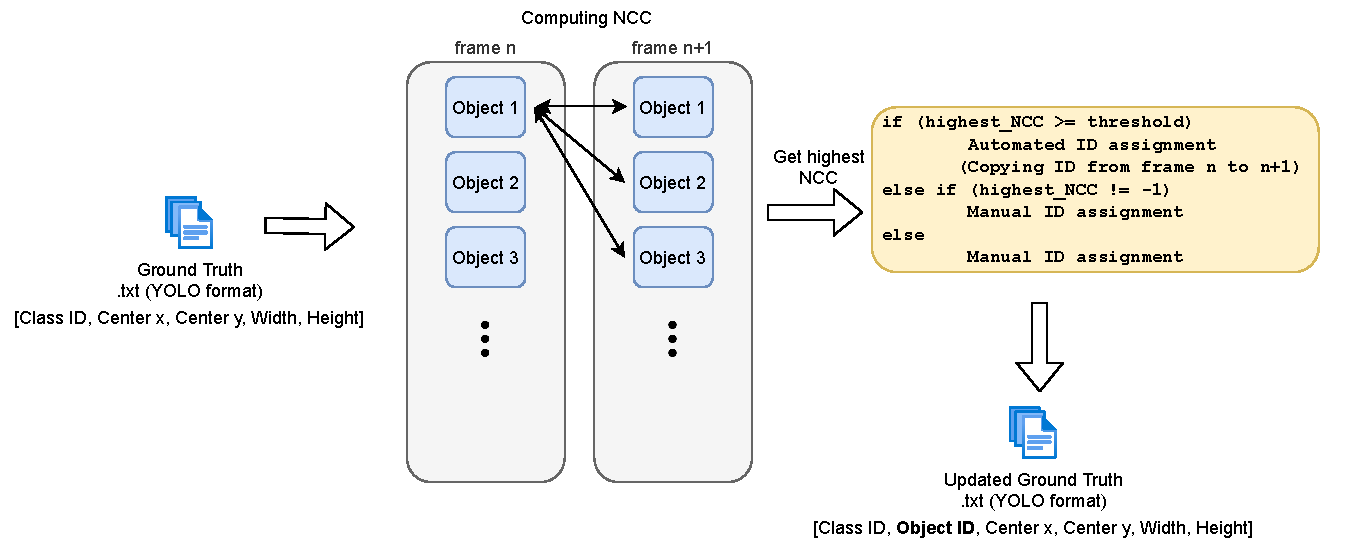
\includegraphics[width=1.0\linewidth]{img/annotation.pdf}
  \caption[Semi-automated annotation process for ID assignment in the ground truth]
  {Semi-automated annotation process for ID assignment in the ground truth.}
  \label{fig:annotation}
\end{figure}
Given the existing ground truth, each object annotation is in the YOLO format as [Class ID, Center x, Center y, Width, Height, Confidence]. Class ID indicates the identifier to the type of object class; for example, "person" as 0, "sports ball" as 32, and "chair" as 56, which are part of the 80 COCO object classes \cite{lin_microsoft_2014}. Center x and Center y are the center position of the bounding box; Width and Height are the corresponding dimensions of boxes. We compared every object in the previous frame $n$ with the current frame $n+1$ and computed NCC values for every possible pair between those image patches of objects. We take the pair of objects that corresponds to the highest NCC value, and if the value is greater than or equal to the threshold, we assign an unique ID automatically but otherwise we manually assign an ID. Threshold is a value that tells how confident the two image patches of objects are similar, and we chose 0.60 for most video sequences. Throughout this semi-automated process of annotation, object IDs are assigned in the second column of ground truth files.
\begin{table}[htb]
    \centering
    \caption{List of Video Sequences adapted from \cite{choi_vcm_2020}}
    \resizebox{1.0\linewidth}{!}{
    \begin{tabular}{|| c | c | c | c | c | c | c ||}
         \hline
          Sequence Class & Sequence Name & Frame Count & Resolution & Object Class IDs & Frame rate (Hz) & Bit depth  \\ [0.5ex]
         \hline\hline
          B & BasketballDrive & 500 & 1920x1080 & [0, 32, 56] & 50 & 8 \\ 
         \hline
          B & Cactus & 500 & 1920x1080 & [58] & 50 & 8 \\ 
         \hline
          B & Kimono & 240 & 1920x1080 & [0, 26] & 24 & 8 \\
         \hline
          B & ParkScene & 240 & 1920x1080 & [0, 1, 13] & 24 & 8 \\
         \hline
          C & BasketballDrill & 500 & 832x480 & [0, 32, 56] & 50 & 8 \\
         \hline
          C & PartyScene & 500 & 832x480 & [0, 41, 58, 74, 77] & 50 & 8 \\
         \hline
          C & RaceHorses & 300 & 832x480 & [0, 17] & 30 & 8 \\
         \hline
          D & BasketballPass & 500 & 416x240 & [0, 32, 56] & 50 & 8 \\
         \hline
          D & BlowingBubbles & 500 & 416x240 & [0, 41, 77] & 50 & 8 \\
          \hline
          D & RaceHorses & 500 & 416x240 & [0, 17] & 30 & 8 \\
          \hline
          E & KristenAndSara & 600 & 1280x720 & [0, 63, 67] & 60 & 8 \\
          \hline
          E & Johnny & 600 & 1280x720 & [0, 27, 63] & 60 & 8 \\
          \hline
          E & FourPeople & 600 & 1280x720 & [0, 41, 56, 58] & 60 & 8 \\
          \hline
    \end{tabular}
    }
    \label{tab:seq_list}
\end{table}
Table \ref{tab:seq_list} shows the 13 uncompressed video sequences for which we created ground truth annotations, out of 18 available video sequences from \cite{choi_vcm_2020}. The sequence class (B, C, D, E) indicates the resolution ($\text{Width} \times \text{Height}$). Each sequence has different number of object classes and each class ID is from the 80 COCO object classes \cite{lin_microsoft_2014}. Table \ref{tab:class_id}, adapted from \cite{choi_vcm_2020}, shows the corresponding object class name for each class ID, and we only listed the object classes that we detect and track in the given sequences from Table \ref{tab:seq_list}.
\begin{table}[!htbp]
    \centering
    \caption{List of Object Class IDs adapted from \cite{choi_vcm_2020}}
    \resizebox{0.6\linewidth}{!}{
    \begin{tabular}{|| c | c | c | c ||}
         \hline
          Class ID & Object class name & Class ID & Object class name \\ [0.5ex]
         \hline\hline
          0 & Person & 41 & Cup \\
         \hline
          1 & Bicycle & 56 & Chair \\
         \hline
         13 & Bench & 58 & Potted plant \\
         \hline
         17 & Horse & 63 & Laptop \\
         \hline
         26 & Handbag & 67 & Cell phone \\
         \hline
         27 & Tie & 74 & Clock \\
         \hline
         32 & Sports ball & 77 & Teddy bear \\
         \hline
    \end{tabular}
    }
    \label{tab:class_id}
\end{table}
In the experiments, "all" refers to all object classes available in the ground truth. The uncompressed sequences are in the YUV420 format. The object tracking pipeline consists of the YOLOv3 detector and SORT, as shown in Figure \ref{fig:yolov3+SORT}. 
\begin{figure}[!htbp]
  \centering
  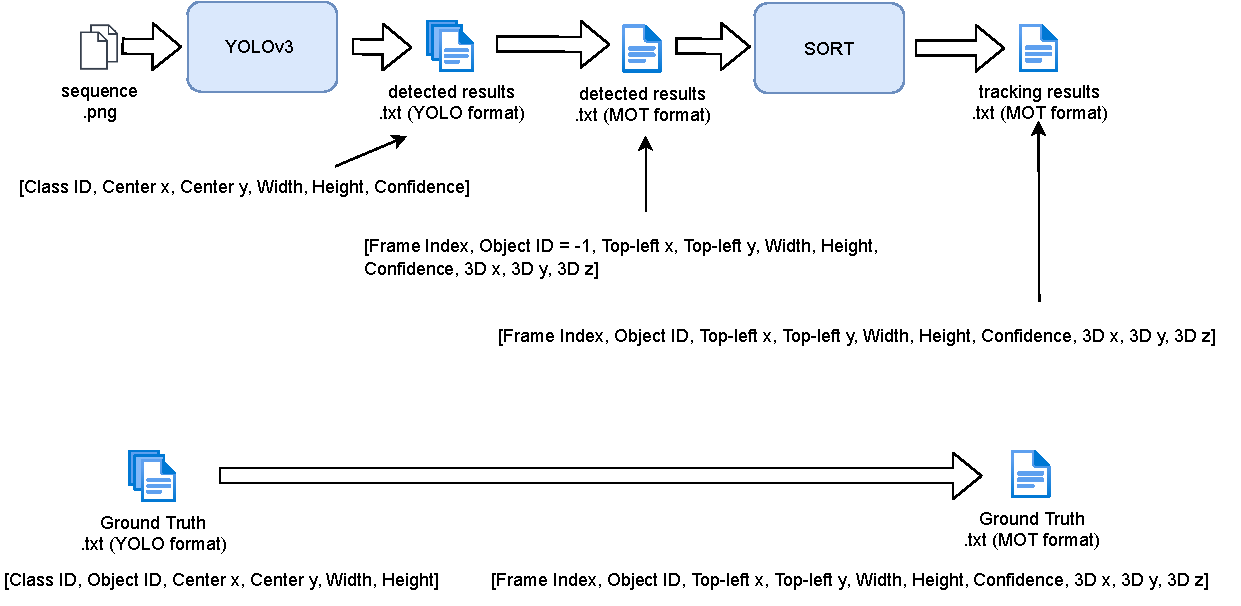
\includegraphics[width=1.0\linewidth]{img/YOLOv3+SORT.pdf}
  \caption[Object tracking pipeline with YOLO v3 and SORT]
  {Object tracking pipeline with YOLO v3 and SORT.}
  \label{fig:yolov3+SORT}
\end{figure}
Input video sequences of PNG files are input to the YOLOv3 object detector. The output from YOLOv3 will be generated in the YOLO format as [Class ID, Center x, Center y, Width, Height, Confidence]. Note that Confidence is the object class probability, and this score tells how confident the object is detected for the particular class. These results are converted to the MOT format used in the \textit{MOTChallenge} 2015 benchmark \cite{leal-taixe_motchallenge_2015}. The object ID, the unique identifier to the object, for the detected result is initialized as -1. Applying SORT to this detected result, we obtain the tracking result in the MOT format with the assigned object ID as [Frame index, Object ID, Top-left x, Top-left y, Width, Height, Confidence, 3D x, 3D y, 3D z]. Top-left x and Top-left y are the positions of the bounding box at the top-left corner. 3D x, 3D y, 3D z is the bounding box position in 3D, but we assigned -1 in our experiment since the 3D position is not applicable to our experiment. The ground truth is also converted from the YOLO format to the MOT format.

% The MOT format from \textit{MOTChallenge} is summarized in 
% \begin{myfont}
% \centering
% Class ID, Object ID, center X, center Y, Width, Height
% \end{myfont}


% \begin{table}[]
%     \centering
%     \caption{}
%     \begin{tabular}{|c|c|}
%         \hline
%         Data field & Description \\
%         \hline\hline
%         Frame Index & Frame index in a sequence \\
%         \hline
%         Object ID & Unique identifier to the object \\
%         \hline
%         Top-left x & x coordinate in top-left corner of the bounding box \\
%         \hline
%         Top-left y & y coordinate in top-left corner of the bounding box \\
%         \hline
%         Width & Width of the bounding box \\
%         \hline
%         Height & Height of the bounding box \\
%         \hline
%         Confidence & Confidence score of the detection of the object \\
%         \hline
%         3D x & x coordinate in 3D bounding box \\
%         \hline
%         3D y & y coordinate in 3D bounding box \\
%         \hline
%         3D z & z coordinate in 3D bounding box \\
%         \hline
%     \end{tabular}
%     \label{tab:MOT_format}
% \end{table}




\section{Insert interesting title (B)}
\label{sec:methods/section_b}

Text goes here.


\section{Experiment Pipeline}
\label{sec:methods/section_c}

Once we selected the parameters for YOLOv3 and SORT, we will run the tracking experiment to assess tracking accuracy. The experiment will involve running the object detector and tracker on the uncompressed and compressed video sequences. For the case of compressed sequences, we apply HEVC video compression (HM16.20) at different quantization parameter (QP) and motion search range (MSR) values. Table \ref{tab:qp_msr_range} shows the range of QP and MSR chosen for the experiment.
\begin{table}[]
    \centering
    \begin{tabular}{|c|c|}
        \hline
        HEVC parameter & Range of values \\
        \hline
        \hline
        QP & [18, 22, 26, 30, 34, 38, 42, 46] \\
        \hline
        MSR & [8, 16, 32, 64] \\
        \hline
    \end{tabular}
    \caption[Selected QP and MSR range for the experiment]
    {Selected QP and MSR range for the experiment.}
    \label{tab:qp_msr_range}
\end{table}
For the case of uncompressed sequences, we do not apply HEVC compression but run the object detector and tracker directly on the sequences. The uncompressed sequences from Table \ref{tab:seq_list} were used, but we excluded the training sequence of PartyScene since we have used this sequence to tune the parameters of the detector and tracker. Therefore, there are a total of 12 sequences in the experiments. Figure \ref{fig:experiment_pipeline} shows the pipeline for the experiment, and each step is explained as follows.

% \begin{myfont}
% \centering
% QP = [18, 22, 26, 30, 34, 38, 42, 46], MSR = [8, 16, 32, 64]
% \end{myfont}


\begin{enumerate}
    \item \textbf{HEVC Encoding}: The experiment starts with applying HEVC encoding to the uncompressed sequences and generating the compressed bitstreams. Low Delay Encoding is used for encoding. Encoding is the process that took the most amount of time in the entire pipeline, so we encoded all the possible combinations of QP and MSR and saved all the compressed bitstreams before applying the decoder.
    \item \textbf{HEVC Decoding}: After obtaining all the compressed bitstreams, we apply the HEVC decoder to the bitstreams and output the decoded sequences in the YUV420 format.
    \item \textbf{YUV420 to RGB24 color conversion}: Since the YOLOv3 object detector accepts in the RGB24 format, we convert the decoded sequences from YUV420 to RGB24 format and save frames in PNG files.
    \item \textbf{Running YOLOv3 and SORT}: Once the decoded sequence are stored in RGB24, we run the object detector and tracker to obtain the tracking results in MOT benchmark format. 
    \item \textbf{MOT metrics evaluation}: To assess the tracking performance, we input both the tracking results and ground truth, and the software \cite{heindl_cheindpy-motmetrics_2021} will generate the tracking performance results.
\end{enumerate}
We ran YOLOv3 and SORT to detect and track each class ID shown in Table \ref{tab:seq_list} as single-class tracking, and also detect and track the "all" object classes. In other words, we took measurements from single-class object tracking and multi-class multiple objects tracking.
\begin{figure}[!htb]
  \centering
  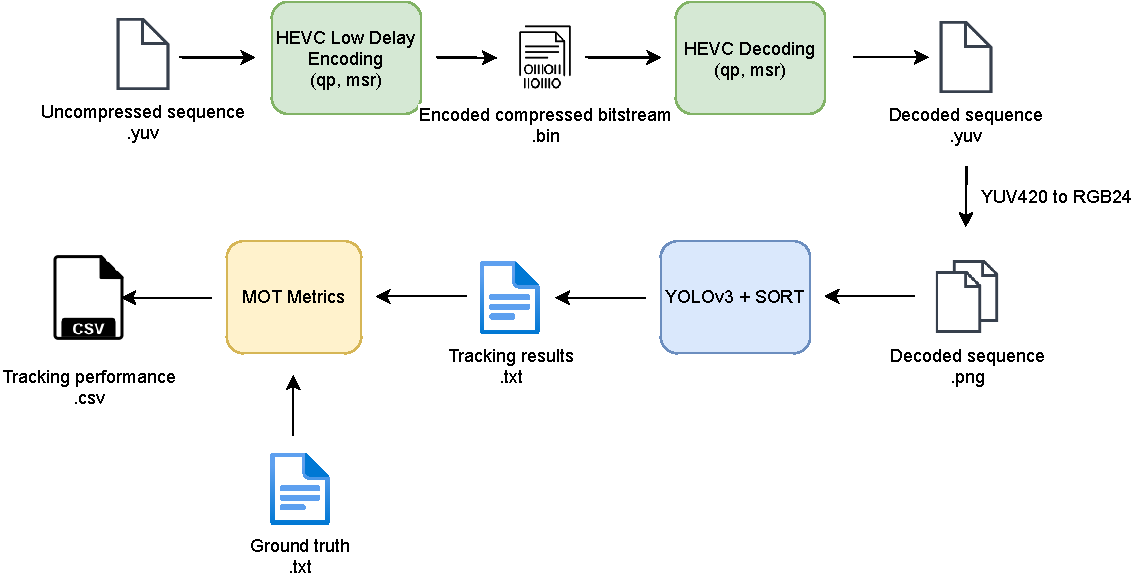
\includegraphics[width=1.0\linewidth]{img/experiment_pipeline.pdf}
  \caption[Pipeline for the experiment]
  {Pipeline for the experiment.}
  \label{fig:experiment_pipeline}
\end{figure}



\section{Summary}
\label{sec:methods/summary}

In this chapter, we described the 13 uncompressed video sequences with the ground truth we generated to run the experiment. The object detection and tracking pipeline with YOLOv3 and SORT were described. The data conversion from the YOLO format to the MOT format was explained. Since there are 6 parameters to be set to run YOLOv3 and SORT, we tuned the parameters on the training sequence to optimize the detector and tracker and determined the suitable values for the parameters before running the main experiment on other sequences. Finally, we explained the experiment pipeline. The pipeline starts with encoding to generate bitstreams, decoding, color conversion, running YOLOv3 and SORT, and evaluating the detection and tracking performance.

\chapter{Results}
\label{chap:results}

A short preview of this chapter.


\section{Results on Multiple Video Sequences}
\label{sec:results/section_a}

Running the experiment with all the possible combinations of QP and MSR as shown in Table \ref{tab:qp_msr_range}, we obtained the result from all 12 video sequences. For each pair of QP and MSR, we averaged each score across all 12 video sequences. As there are 20 metrics for evaluating object tracking performance, and MOTA is a good indicator of the overall tracking performance as explained in Section \ref{sec:background/section_d}, we focused our study on MOTA. In the following analysis, we visualized the data and conducted a regression analysis and t-test to quantify the results. The methodologies of statistical analysis we employed are according to the textbook \cite{kutner_applied_2005}.

% ----------------------------------------------------------
% Visualization
% ----------------------------------------------------------

\subsection{Visualization of Results across All Video Sequences}
\label{subsec:/results/section_a/visualization}
We visualized the MOTA score for "all" object classes across all video sequences at different QP and MSR as shown in Figure \ref{fig:averaged_result_all_qp}.
\begin{figure}[!htbp]
  \centering
  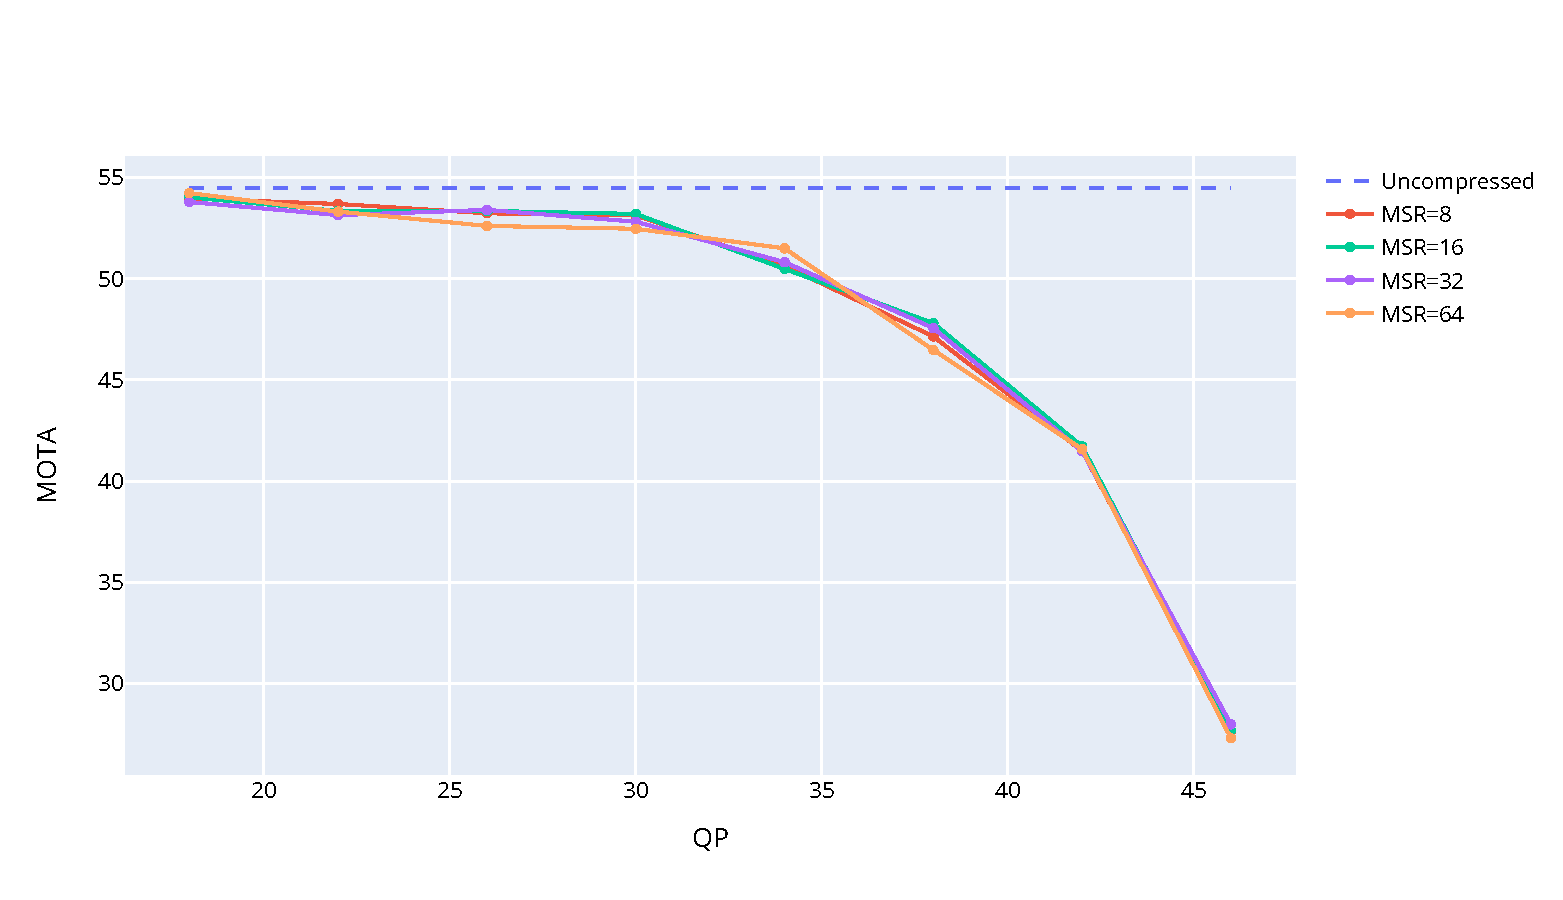
\includegraphics[width=1.0\linewidth]{img/averaged_result_all_qp.pdf}
  \caption[Averaged Result of All Video Samples with All Object Classes]{
    
  }
  \label{fig:averaged_result_all_qp}
\end{figure}
As can be seen from the plot, the uncompressed video sequences achieved the highest MOTA score on average. For the compressed sequences, the average MOTA score is lower than the uncompressed result, and the higher the QP, the lower the MOTA score. Not only MOTA, we observed that the performance scores of most of the other metrics decrease as QP increases. Although the scores at different MSR are shown, we do not see any significant differences between MOTA scores at different MSR values from this plot.

Figure \ref{fig:averaged_result_all_multiplots_qp} shows the visualization of all the metrics\footnote{The metric GT is omitted from the visualization since it is a constant value, and the value can be confirmed from the table.} over different QP and MSR, and Table \ref{tab:averaged_result_all} tabulates their values.
\begin{figure}[!htbp]
  \centering
  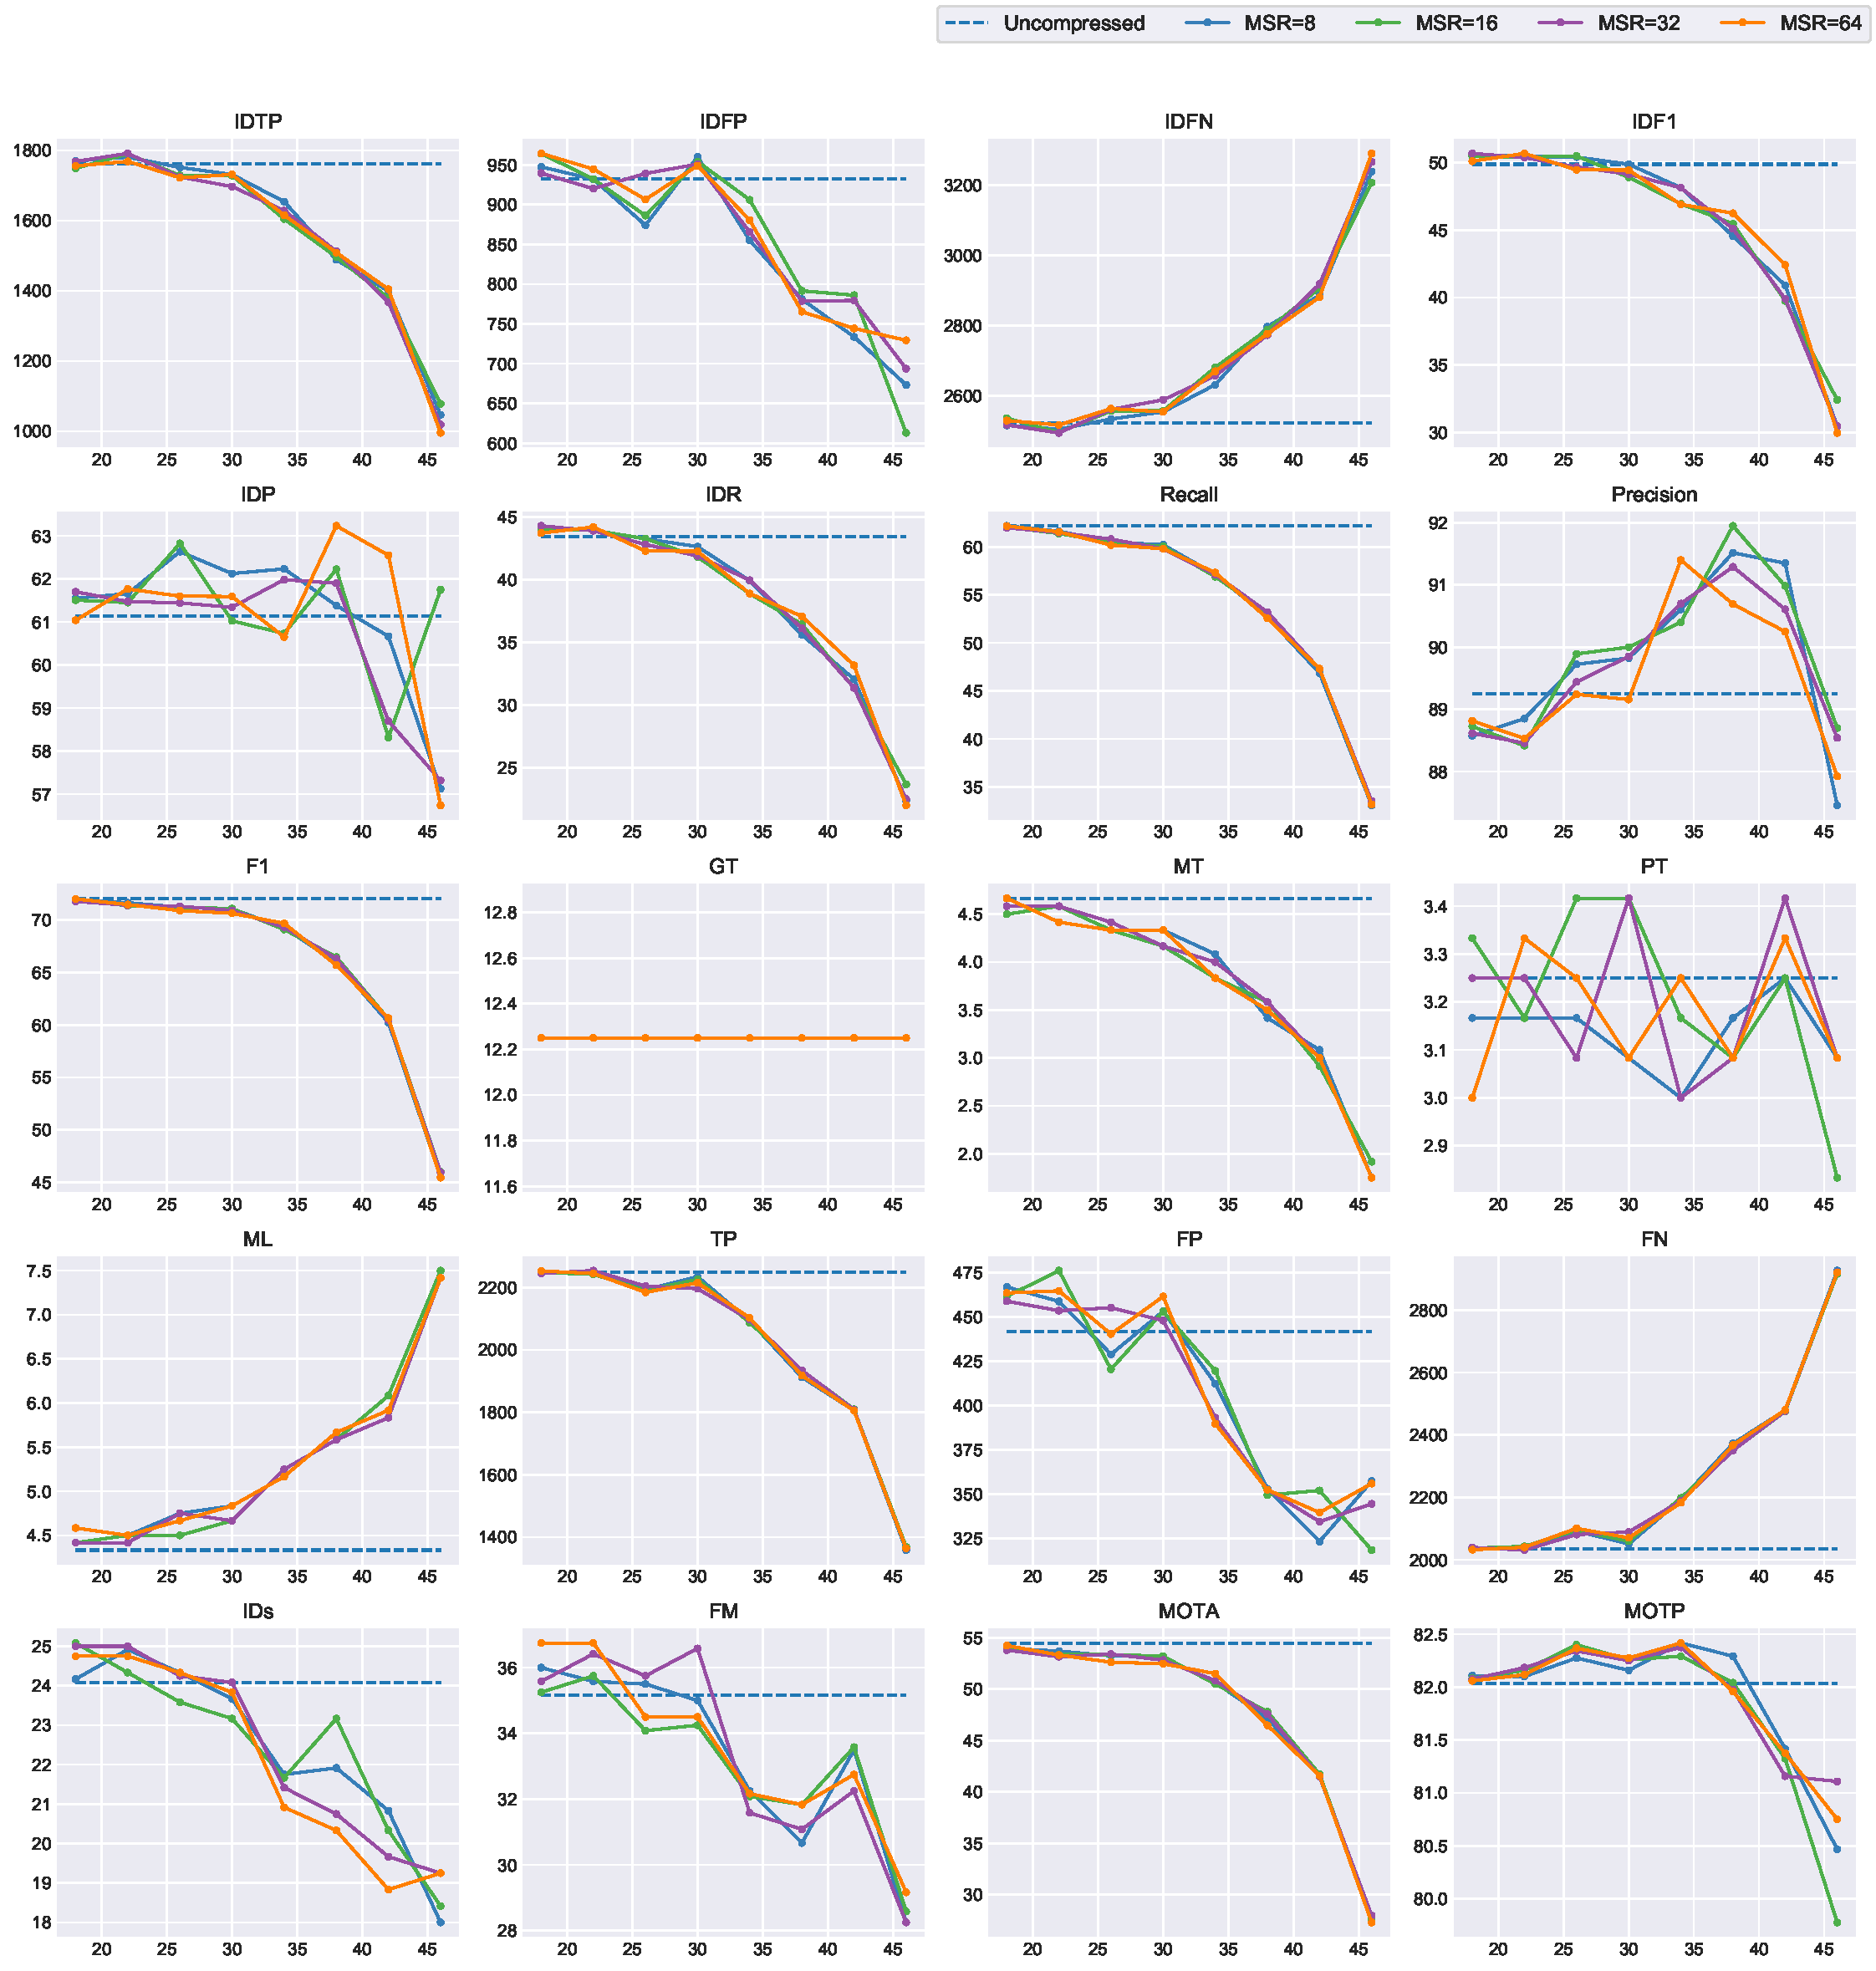
\includegraphics[width=1.0\linewidth]{img/averaged_all_multiplots_qp.pdf}
  \caption[Averaged Result of All Video Samples with All Object Classes]{
    
  }
  \label{fig:averaged_result_all_multiplots_qp}
\end{figure}
\begin{table}[!htbp]
  \centering
  \caption[Averaged performance results of all video samples]
  {Averaged performance results of all video samples.}

  % table for uncompressed
  \begin{subtable}[t]{\linewidth}
    \centering
    \vspace{0pt}
    \resizebox{1.0\linewidth}{!}{
    \begin{tabular}{llrrrrrrrrrrrrrrrrrrrr}
    \toprule
              QP &          MSR &    IDTP &   IDFP &    IDFN &  IDF1 &   IDP &   IDR &  Recall &  Precision &    F1 &    GT &   MT &   PT &   ML &      TP &     FP &      FN &   IDs &    FM &  MOTA &  MOTP \\
    \midrule
    Uncompressed & Uncompressed & 1762.58 & 932.83 & 2522.67 & 49.88 & 61.13 & 43.48 &   62.17 &      89.25 & 72.08 & 12.25 & 4.67 & 3.25 & 4.33 & 2249.75 & 441.67 & 2035.50 & 24.08 & 35.17 & 54.49 & 82.03 \\
    \bottomrule
    \end{tabular}}
    \caption{Mean values for the uncompressed sequence}
  \end{subtable}
 
 
 
  
  % table for msr=8
  \begin{subtable}[t]{\linewidth}
    \centering
    \resizebox{1.0\linewidth}{!}{
    \begin{tabular}{rrrrrrrrrrrrrrrrrrrrrr}
    \toprule
     QP &  MSR &    IDTP &   IDFP &    IDFN &  IDF1 &   IDP &   IDR &  Recall &  Precision &    F1 &    GT &   MT &   PT &   ML &      TP &     FP &      FN &   IDs &    FM &  MOTA &  MOTP \\
    \midrule
     18 &    8 & 1770.08 & 947.50 & 2515.17 & 50.60 & 61.55 & 44.26 &   62.18 &      88.58 & 71.92 & 12.25 & 4.50 & 3.17 & 4.58 & 2246.75 & 466.83 & 2038.50 & 24.17 & 36.00 & 53.97 & 82.11 \\
     22 &    8 & 1780.83 & 931.92 & 2504.42 & 50.46 & 61.66 & 43.96 &   61.62 &      88.85 & 71.65 & 12.25 & 4.58 & 3.17 & 4.50 & 2250.00 & 458.75 & 2035.25 & 24.92 & 35.58 & 53.70 & 82.10 \\
     26 &    8 & 1751.67 & 874.17 & 2533.58 & 50.41 & 62.63 & 43.28 &   60.49 &      89.73 & 71.22 & 12.25 & 4.33 & 3.17 & 4.75 & 2192.92 & 428.92 & 2092.33 & 24.33 & 35.50 & 53.24 & 82.28 \\
     30 &    8 & 1731.50 & 960.08 & 2553.75 & 49.88 & 62.12 & 42.65 &   60.21 &      89.83 & 71.07 & 12.25 & 4.33 & 3.08 & 4.83 & 2234.42 & 453.17 & 2050.83 & 23.67 & 35.00 & 53.13 & 82.16 \\
     34 &    8 & 1653.92 & 855.08 & 2631.33 & 48.14 & 62.23 & 39.93 &   57.12 &      90.61 & 69.26 & 12.25 & 4.08 & 3.00 & 5.17 & 2092.58 & 412.42 & 2192.67 & 21.75 & 32.25 & 50.64 & 82.42 \\
     38 &    8 & 1488.50 & 781.08 & 2796.75 & 44.56 & 61.38 & 35.62 &   52.70 &      91.52 & 65.97 & 12.25 & 3.42 & 3.17 & 5.67 & 1912.42 & 353.17 & 2372.83 & 21.92 & 30.67 & 47.15 & 82.29 \\
     42 &    8 & 1399.25 & 733.83 & 2886.00 & 40.92 & 60.67 & 32.08 &   46.86 &      91.35 & 60.24 & 12.25 & 3.08 & 3.25 & 5.92 & 1805.67 & 323.42 & 2479.58 & 20.83 & 33.50 & 41.48 & 81.42 \\
     46 &    8 & 1046.50 & 673.33 & 3238.75 & 30.48 & 57.12 & 22.40 &   33.09 &      87.46 & 45.48 & 12.25 & 1.75 & 3.08 & 7.42 & 1358.33 & 357.50 & 2926.92 & 18.00 & 28.25 & 27.64 & 80.47 \\
    \bottomrule
    \end{tabular}}
    \caption{Mean values for MSR = 8}
  \end{subtable}
 
 
  
  % table for msr=16
  \begin{subtable}[t]{\linewidth}
    \centering
    \resizebox{1.0\linewidth}{!}{
    \begin{tabular}{rrrrrrrrrrrrrrrrrrrrrr}
    \toprule
     QP &  MSR &    IDTP &   IDFP &    IDFN &  IDF1 &   IDP &   IDR &  Recall &  Precision &    F1 &    GT &   MT &   PT &   ML &      TP &     FP &      FN &   IDs &    FM &  MOTA &  MOTP \\
    \midrule
     18 &   16 & 1749.25 & 964.25 & 2536.00 & 50.48 & 61.51 & 44.07 &   62.04 &      88.73 & 71.88 & 12.25 & 4.50 & 3.33 & 4.42 & 2248.00 & 461.50 & 2037.25 & 25.08 & 35.25 & 54.03 & 82.08 \\
     22 &   16 & 1790.08 & 932.17 & 2495.17 & 50.40 & 61.45 & 43.96 &   61.39 &      88.42 & 71.38 & 12.25 & 4.58 & 3.17 & 4.50 & 2242.17 & 476.08 & 2043.08 & 24.33 & 35.75 & 53.36 & 82.16 \\
     26 &   16 & 1728.75 & 886.25 & 2556.50 & 50.48 & 62.82 & 43.28 &   60.43 &      89.89 & 71.21 & 12.25 & 4.33 & 3.42 & 4.50 & 2190.50 & 420.50 & 2094.75 & 23.58 & 34.08 & 53.36 & 82.40 \\
     30 &   16 & 1728.33 & 954.08 & 2556.92 & 48.91 & 61.02 & 41.83 &   60.04 &      90.00 & 71.10 & 12.25 & 4.17 & 3.42 & 4.67 & 2225.42 & 453.00 & 2059.83 & 23.17 & 34.25 & 53.21 & 82.26 \\
     34 &   16 & 1604.67 & 906.00 & 2680.58 & 46.94 & 60.73 & 38.90 &   56.89 &      90.40 & 69.10 & 12.25 & 3.83 & 3.17 & 5.25 & 2087.08 & 419.58 & 2198.17 & 21.67 & 32.08 & 50.49 & 82.29 \\
     38 &   16 & 1496.58 & 791.58 & 2788.67 & 45.47 & 62.23 & 36.46 &   53.13 &      91.95 & 66.47 & 12.25 & 3.58 & 3.08 & 5.58 & 1934.58 & 349.58 & 2350.67 & 23.17 & 31.83 & 47.81 & 82.04 \\
     42 &   16 & 1379.33 & 786.17 & 2905.92 & 39.76 & 58.32 & 31.38 &   47.28 &      90.98 & 60.56 & 12.25 & 2.92 & 3.25 & 6.08 & 1809.33 & 352.17 & 2475.92 & 20.33 & 33.58 & 41.72 & 81.33 \\
     46 &   16 & 1078.17 & 613.00 & 3207.08 & 32.42 & 61.75 & 23.68 &   33.48 &      88.70 & 45.99 & 12.25 & 1.92 & 2.83 & 7.50 & 1368.58 & 318.58 & 2916.67 & 18.42 & 28.58 & 27.67 & 79.77 \\
    \bottomrule
    \end{tabular}}
    \caption{Mean values for MSR = 16}
  \end{subtable}
 
 
 
  % table for msr=32
  \begin{subtable}[t]{\linewidth}
    \centering
    \resizebox{1.0\linewidth}{!}{
    \begin{tabular}{rrrrrrrrrrrrrrrrrrrrrr}
    \toprule
     QP &  MSR &    IDTP &   IDFP &    IDFN &  IDF1 &   IDP &   IDR &  Recall &  Precision &    F1 &    GT &   MT &   PT &   ML &      TP &     FP &      FN &   IDs &    FM &  MOTA &  MOTP \\
    \midrule
     18 &   32 & 1768.58 & 939.58 & 2516.67 & 50.67 & 61.70 & 44.31 &   61.98 &      88.62 & 71.78 & 12.25 & 4.58 & 3.25 & 4.42 & 2245.33 & 458.83 & 2039.92 & 25.00 & 35.58 & 53.80 & 82.08 \\
     22 &   32 & 1791.42 & 920.08 & 2493.83 & 50.38 & 61.48 & 43.92 &   61.49 &      88.46 & 71.42 & 12.25 & 4.58 & 3.25 & 4.42 & 2254.00 & 453.50 & 2031.25 & 25.00 & 36.42 & 53.15 & 82.18 \\
     26 &   32 & 1724.42 & 939.08 & 2560.83 & 49.68 & 61.44 & 42.82 &   60.80 &      89.44 & 71.32 & 12.25 & 4.42 & 3.08 & 4.75 & 2204.33 & 455.17 & 2080.92 & 24.25 & 35.75 & 53.41 & 82.34 \\
     30 &   32 & 1697.08 & 950.92 & 2588.17 & 49.14 & 61.34 & 41.91 &   59.79 &      89.85 & 70.91 & 12.25 & 4.17 & 3.42 & 4.67 & 2196.08 & 447.92 & 2089.17 & 24.08 & 36.58 & 52.83 & 82.25 \\
     34 &   32 & 1628.42 & 865.50 & 2656.83 & 48.13 & 61.98 & 39.98 &   57.10 &      90.70 & 69.32 & 12.25 & 4.00 & 3.00 & 5.25 & 2096.75 & 393.17 & 2188.50 & 21.42 & 31.58 & 50.83 & 82.38 \\
     38 &   32 & 1512.50 & 778.75 & 2772.75 & 45.10 & 61.90 & 36.13 &   53.20 &      91.29 & 66.31 & 12.25 & 3.58 & 3.08 & 5.58 & 1934.67 & 352.58 & 2350.58 & 20.75 & 31.08 & 47.57 & 81.98 \\
     42 &   32 & 1367.25 & 779.58 & 2918.00 & 39.92 & 58.70 & 31.38 &   47.28 &      90.61 & 60.48 & 12.25 & 3.00 & 3.42 & 5.83 & 1808.25 & 334.58 & 2477.00 & 19.67 & 32.25 & 41.48 & 81.16 \\
     46 &   32 & 1018.67 & 693.75 & 3266.58 & 30.47 & 57.32 & 22.52 &   33.53 &      88.54 & 45.93 & 12.25 & 1.75 & 3.08 & 7.42 & 1363.75 & 344.67 & 2921.50 & 19.25 & 28.25 & 27.97 & 81.11 \\
    \bottomrule
    \end{tabular}}
    \caption{Mean values for MSR = 32}
  \end{subtable}
  
  
  % table for msr=64
  \begin{subtable}[t]{\linewidth}
    \centering
    \resizebox{1.0\linewidth}{!}{
    \begin{tabular}{rrrrrrrrrrrrrrrrrrrrrr}
    \toprule
     QP &  MSR &    IDTP &   IDFP &    IDFN &  IDF1 &   IDP &   IDR &  Recall &  Precision &    F1 &    GT &   MT &   PT &   ML &      TP &     FP &      FN &   IDs &    FM &  MOTA &  MOTP \\
    \midrule
     18 &   64 & 1756.00 & 964.33 & 2529.25 & 50.10 & 61.04 & 43.73 &   62.17 &      88.82 & 72.02 & 12.25 & 4.67 & 3.00 & 4.58 & 2252.83 & 463.50 & 2032.42 & 24.75 & 36.75 & 54.24 & 82.06 \\
     22 &   64 & 1768.75 & 944.75 & 2516.50 & 50.68 & 61.77 & 44.22 &   61.56 &      88.53 & 71.48 & 12.25 & 4.42 & 3.33 & 4.50 & 2244.83 & 464.67 & 2040.42 & 24.75 & 36.75 & 53.33 & 82.12 \\
     26 &   64 & 1722.25 & 906.50 & 2563.00 & 49.46 & 61.60 & 42.30 &   60.18 &      89.24 & 70.90 & 12.25 & 4.33 & 3.25 & 4.67 & 2184.42 & 440.33 & 2100.83 & 24.33 & 34.50 & 52.62 & 82.37 \\
     30 &   64 & 1731.25 & 949.00 & 2554.00 & 49.44 & 61.59 & 42.27 &   59.80 &      89.16 & 70.64 & 12.25 & 4.33 & 3.08 & 4.83 & 2214.75 & 461.50 & 2070.50 & 23.83 & 34.50 & 52.47 & 82.28 \\
     34 &   64 & 1615.58 & 880.42 & 2669.67 & 46.90 & 60.65 & 38.91 &   57.32 &      91.40 & 69.69 & 12.25 & 3.83 & 3.25 & 5.17 & 2102.25 & 389.75 & 2183.00 & 20.92 & 32.17 & 51.51 & 82.42 \\
     38 &   64 & 1508.92 & 765.42 & 2776.33 & 46.25 & 63.23 & 37.09 &   52.56 &      90.69 & 65.69 & 12.25 & 3.50 & 3.08 & 5.67 & 1917.75 & 352.58 & 2367.50 & 20.33 & 31.83 & 46.48 & 81.96 \\
     42 &   64 & 1404.50 & 744.42 & 2880.75 & 42.43 & 62.55 & 33.18 &   47.31 &      90.25 & 60.65 & 12.25 & 3.00 & 3.33 & 5.92 & 1805.17 & 339.75 & 2480.08 & 18.83 & 32.75 & 41.57 & 81.38 \\
     46 &   64 &  995.00 & 729.42 & 3290.25 & 29.98 & 56.74 & 22.02 &   33.18 &      87.92 & 45.43 & 12.25 & 1.75 & 3.08 & 7.42 & 1364.33 & 356.08 & 2920.92 & 19.25 & 29.17 & 27.29 & 80.75 \\
    \bottomrule
    \end{tabular}}
    \caption{Mean values for MSR = 64}
  \end{subtable}

  
\label{tab:averaged_result_all}  
\end{table}
As discussed in Section \ref{sec:background/section_e}, the higher the QP, the lower the bitrate, so we expected the tracking performance to be lower. Our performance results from most metrics are consistent with this expectation. To explain the decrease of MOTA defined in terms of FP, FN, and IDs based on Equation \eqref{eqn:MOTA}, we can see that as QP increases, FP and IDs decreases but FN increases, which is consistent with our expectation. Although the decrease of FP and IDs contribute to the increase of MOTA, the increase of FN is significantly larger than FP and IDs; thus, MOTA decreases. However, we observed that Precision and MOTP are not entirely consistent with our expectation and that the performance first increases and then decreases as QP is increased. Since video samples differ in resolution, frame rate, number of objects, and object classes, tracking performance is different. Due to the relatively small number of video samples, the standard deviation is relatively high around the average performance. We show standard deviations in Appendix \ref{sec:appendix/section_std_dev}. To see if MSR impacts the performance scores, we visualized each performance score versus MSR as a horizontal axis, and we observed no significant dependence on MSR as shown in Figure \ref{fig:averaged_result_all_multiplots_msr}.
\begin{figure}[!htbp]
  \centering
  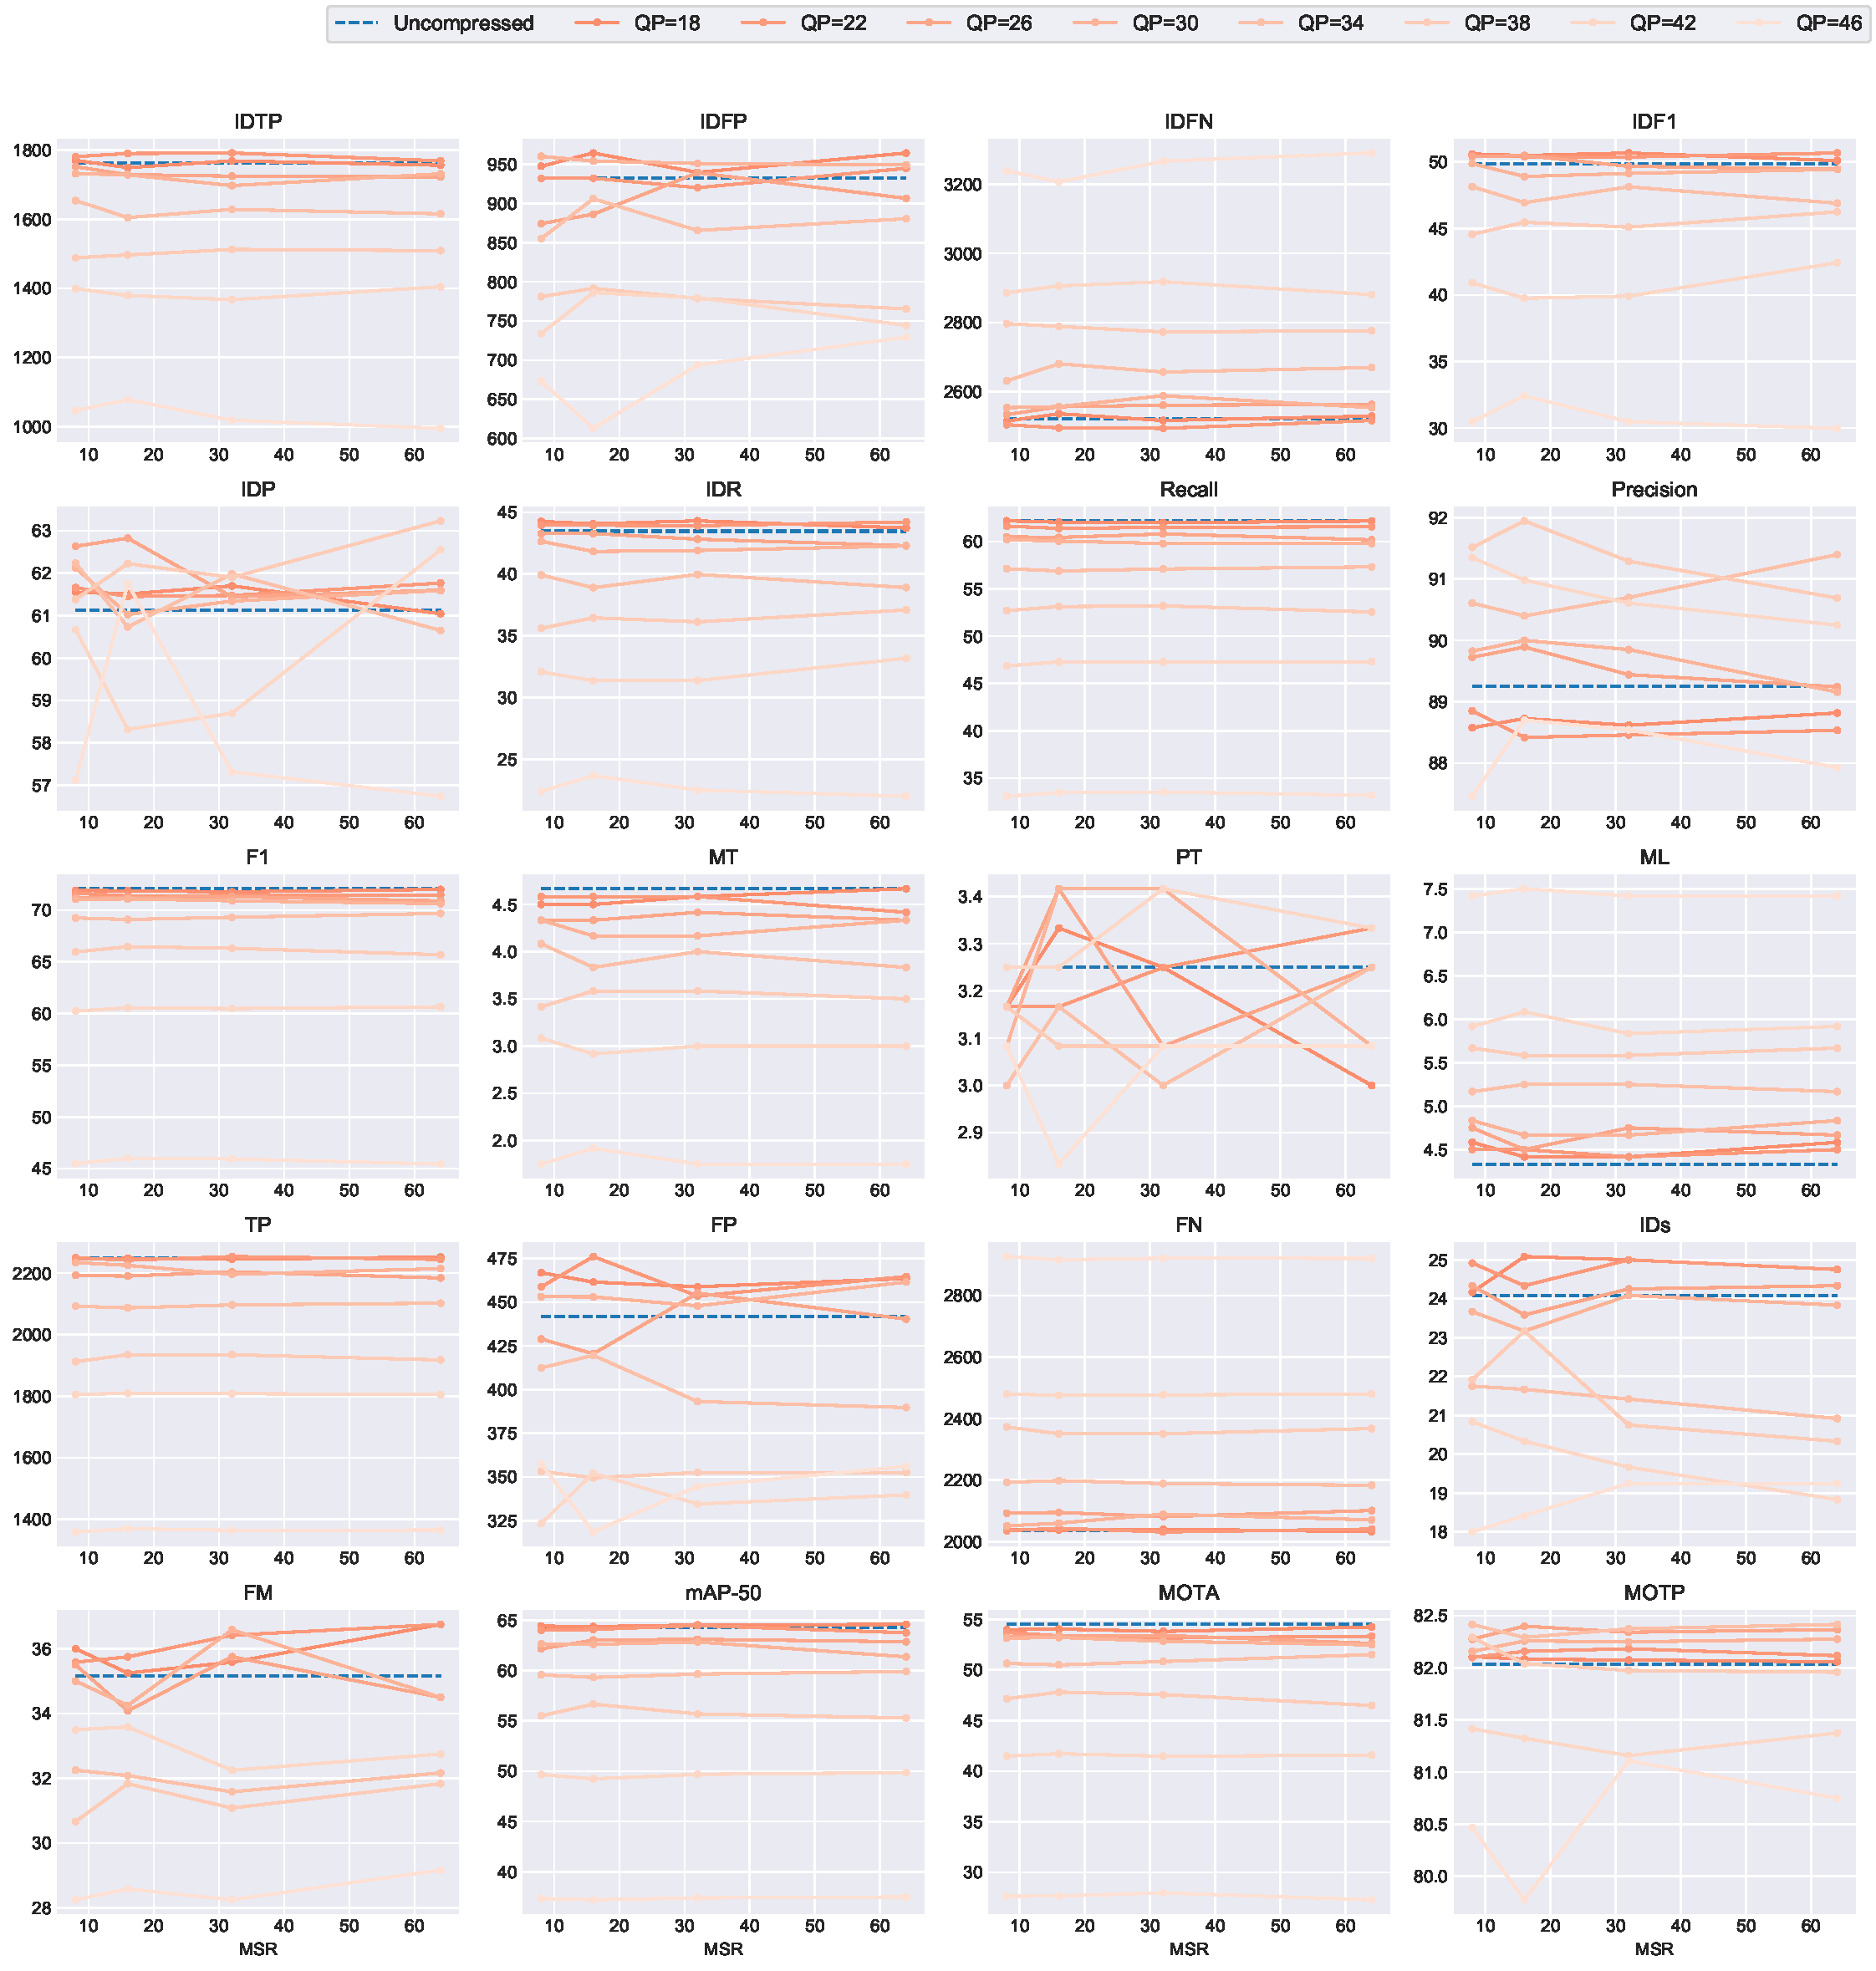
\includegraphics[width=1.0\linewidth]{img/averaged_all_multiplots_msr.pdf}
  \caption[Visualization of the averaged performance results at different MSR of all video samples]
  {Visualization of the average performance results at different MSR across all video samples.}
  \label{fig:averaged_result_all_multiplots_msr}
\end{figure}

% ----------------------------------------------------------
% Regression Analysis
% ----------------------------------------------------------

\subsection{Regression Analysis}
\label{subsec:/results/section_a/regression_analysis}
To examine the impact of QP and MSR on tracking accuracy quantitatively, we conducted a regression analysis on the entire data (all the video sequences). As we focused on the analysis on the MOTA score, we quantified the result on MOTA over QP and MSR values. As can be seen from the visualization, the relationship between MOTA and MSR is constant, but MOTA does change with QP. In order to conduct linear regression analysis, we transformed QP so that the relationship between MOTA and $\text{QP}'$ is more linear (we call the transformed QP as $\text{QP}'$). The determination of the exact QP transformation was found by plotting various forms of transformation on the scatter plots on the individual video sequences by trial and error. The factor 52 was chosen in the denominator because since QP ranges from 0 to 51 in theory \cite{sullivan_overview_2012} and if choose 51 as a factor, QP at 51 will be undefined. To avoid this issue, we chose the factor 52. Figure \ref{fig:QP_transformation} shows the scatter plots of MOTA before and after the chosen QP transformation on the example sequence BasketballPass. Using the form of Equation \eqref{eqn:QP_transformation}, the scatter plot of MOTA at different $\text{QP}'$ shows a linear relationship, as shown in Figure \ref{fig:QP_transformation_after}. Similar outcomes were observed in other video sequences as well.
% \begin{figure}[!tb]
%   \centering
%   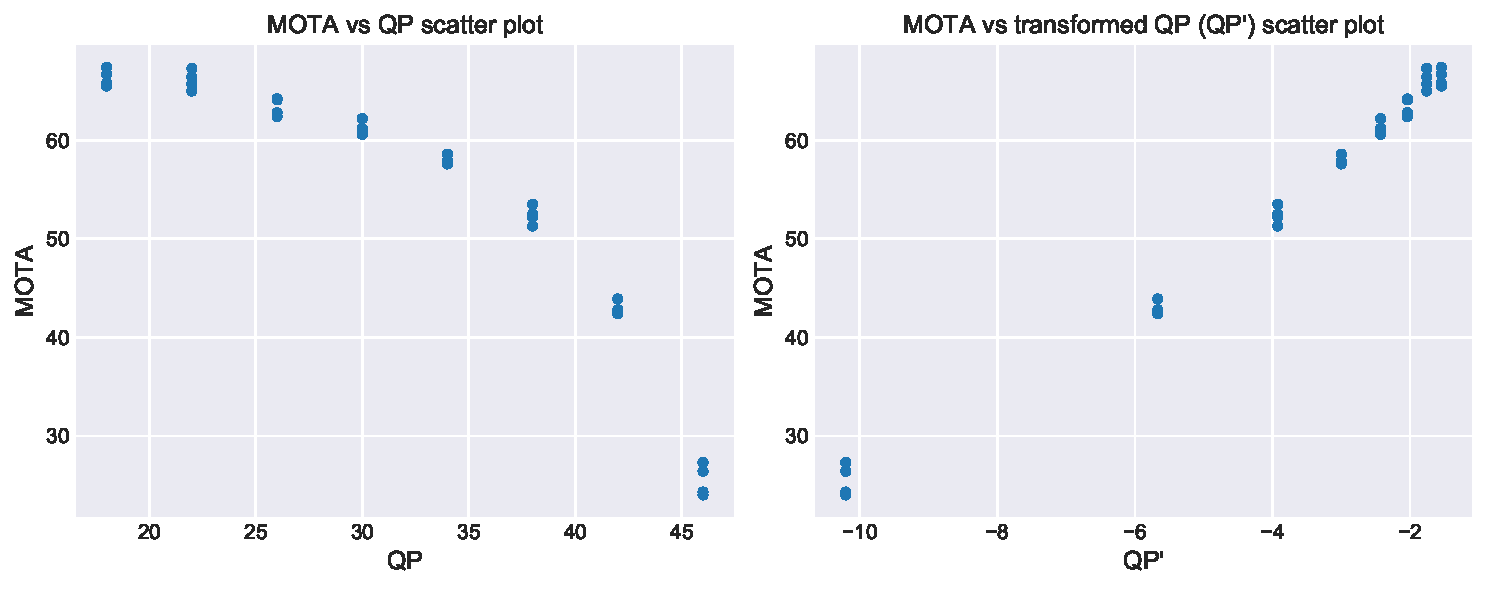
\includegraphics[width=1.0\linewidth]{img/QP_transformation.pdf}
%   \caption[Scatter plots before and after the QP transformation]
%   {Scatter plots before and after the QP transformation.}
%   \label{fig:QP_transformation}
% \end{figure}

\begin{figure}[!tb]
  \centering
  \begin{subfigure}[b]{.5\textwidth}
    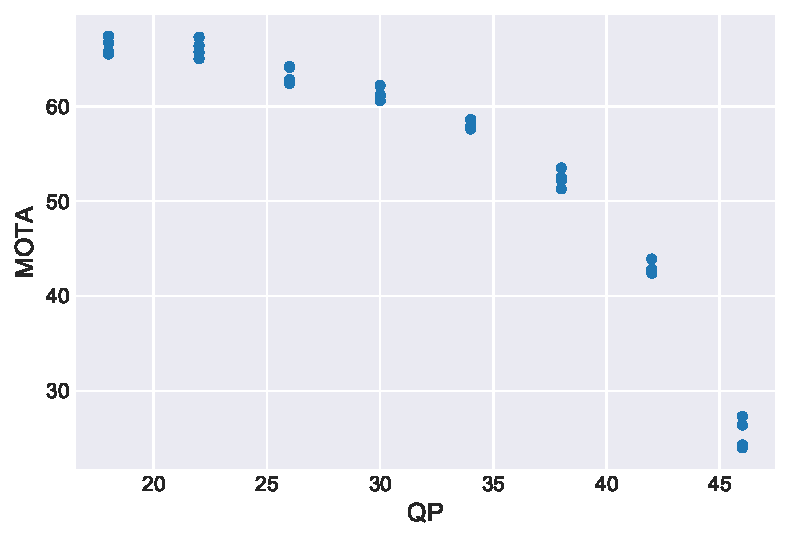
\includegraphics[width=\textwidth]{img/QP_transformation_before.pdf}
    \caption{MOTA vs QP scatter plot}
    \label{fig:QP_transformation_before}
  \end{subfigure}%
  \begin{subfigure}[b]{.5\textwidth}
    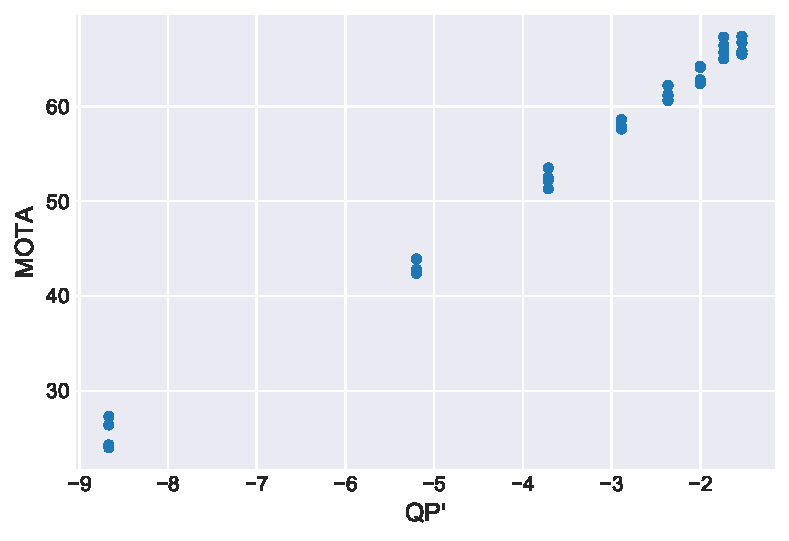
\includegraphics[width=\textwidth]{img/QP_transformation_after.pdf}
    \caption{MOTA vs $\text{QP}'$ scatter plot}
    \label{fig:QP_transformation_after}
  \end{subfigure}
  \caption[Scatter plots before and after the QP transformation on the BasketballPass sequence]{%
    Scatter plots before and after the QP transformation on the BasketballPass sequence.%
  }
  \label{fig:QP_transformation}
\end{figure}
\begin{equation}
\text{QP}' =  \frac{1}{\frac{\text{QP}}{52}-1}
\label{eqn:QP_transformation}
\end{equation}
However, using all the video sequences, which have different MOTA scores, the variance at each $\text{QP}'$ is high, and little insight can be derived from the high variance of data as shown in Figure \ref{fig:MOTA_transformation_before}. Therefore, we transformed MOTA such that we subtract each MOTA score at different $\text{QP}'$ from the uncompressed MOTA score, as represented below.
% \begin{figure}[!tb]
%   \centering
%   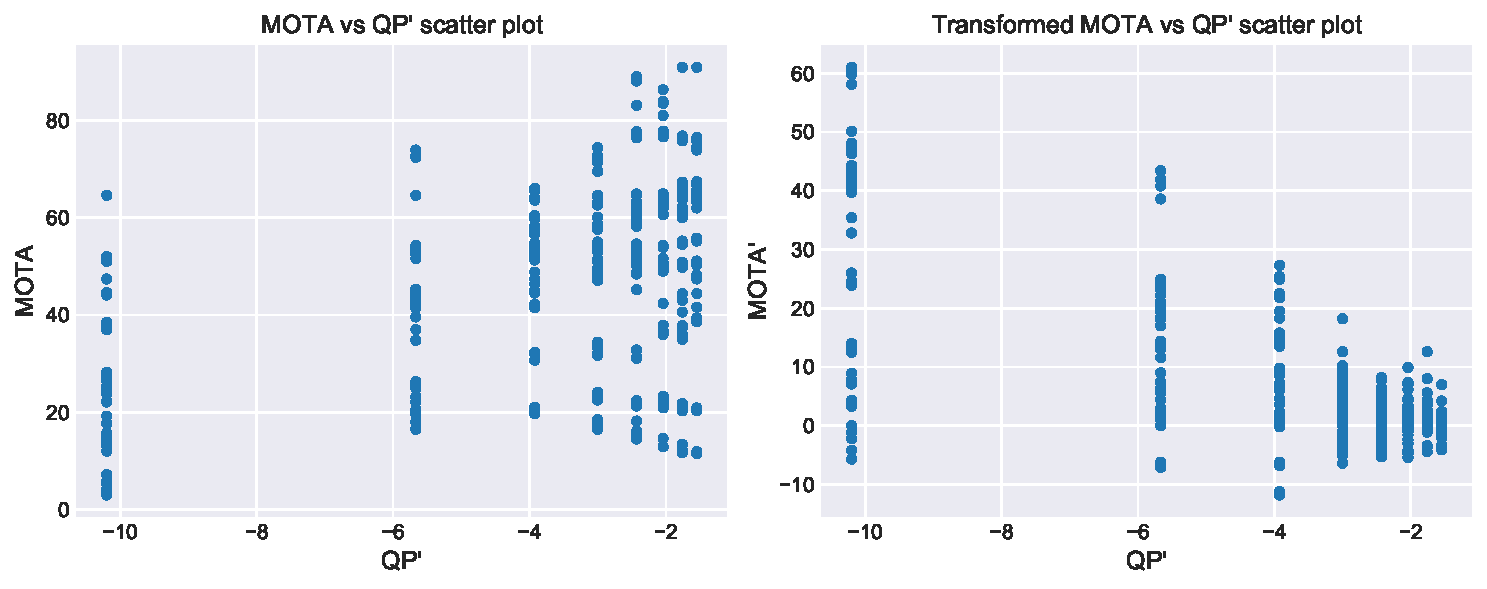
\includegraphics[width=1.0\linewidth]{img/MOTA_transformation.pdf}
%   \caption[Scatter plots before and after the MOTA transformation]
%   {Scatter plots before and after the MOTA transformation.}
%   \label{fig:MOTA_transformation}
% \end{figure}

% spacing between subfigures will not align the sub figures horizontanlly

\begin{figure}[!tb]
  \centering
  \begin{subfigure}{.5\linewidth}
    \centering
    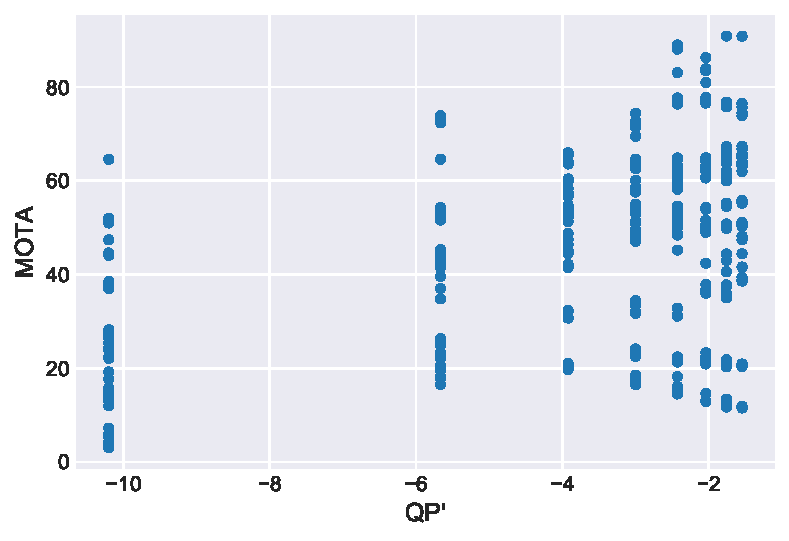
\includegraphics[width=\linewidth]{img/MOTA_transformation_before.pdf}
    \caption{MOTA vs $\text{QP}'$ scatter plot}
    \label{fig:MOTA_transformation_before}
  \end{subfigure}%
  \begin{subfigure}{.5\linewidth}
    \centering
    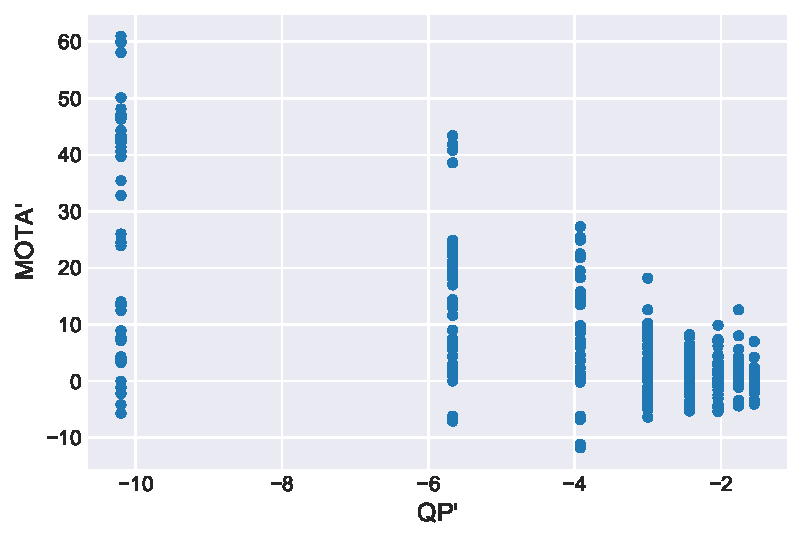
\includegraphics[width=\linewidth]{img/MOTA_transformation_after.pdf}
    \caption{$\text{MOTA}'$ vs $\text{QP}'$ scatter plot }
    \label{fig:MOTA_transformation_after}
  \end{subfigure}
  \caption[Scatter plots before and after the MOTA transformation on all the video sequences]{%
    Scatter plots before and after the MOTA transformation across all the video sequences.%
  }
  \label{fig:MOTA_transformation}
\end{figure}

\begin{equation}
\text{MOTA}_i' = \text{MOTA(Uncompressed)} -  \text{MOTA}(\text{QP}_i)
\label{eqn:MOTA_transformation}
\end{equation}
Doing this transformation, we only consider the drop of the MOTA score from the uncompressed sequence, and the variance is lower at higher $\text{QP}'$, in other words, the variance is lower at lower QP. This is expected because $\text{MOTA(Uncompressed)}$ and $\text{MOTA}(\text{QP}_i)$ are both random variables, and the difference of these two variables will be lower at lower QP. Figure \ref{fig:MOTA_transformation_after} shows the scatter plot of all the video sequences after the MOTA transformation. We can see from this figure that the relationship between $\text{MOTA}'$ and $\text{QP}'$ is still linear but error variance at each $\text{QP}'$ is not constant. Therefore, the weighted least squares method is adopted in the regression model. Also, since we have two continuous independent variables of $\text{QP}'$ and MSR and each may impact the continuous response variable of the $\text{MOTA}'$ score, we applied a multiple linear regression across all the video sequences. We represent the regression model as,
\begin{equation}
\text{MOTA}'_i = \beta_0 + \beta_1 \cdot \text{QP}'_i + \beta_2 \cdot \text{MSR}_i + \beta_3 \cdot \text{QP}'_i \cdot \text{MSR}_i + \epsilon_i~,
\label{eqn:regression_model}
\end{equation}
where $\beta_0$ is the intercept; $\beta_1$ and $\beta_2$ are the parameters of independent variables $\text{QP}'$ and MSR; $\beta_3$ is the parameter of the interaction term of $\text{QP}'$ and MSR. The interaction term is included to see if MSR and $\text{QP}'$ depend on each other. We assume that $\epsilon_i$ is the independent normally distributed error with mean 0 and variance $\sigma^2_i$, where $i$ indicates the $i$-th trial from the independent variables. As we are applying the weighted least squares method, the weight at each $\text{QP}'$ can be calculated as
\begin{equation}
    w_i = \frac{1}{\sigma^2_i}
    \label{eqn:weight}
\end{equation}
Equation \eqref{eqn:weight} is according to \cite[p.~422]{kutner_applied_2005}. Since $\sigma_i$ is the true value of standard deviation at each $\text{QP}'$, we estimate $w_i$ using the sample standard deviation $s_i$ of data points at each $\text{QP}'$:
\begin{equation}
    w_i = \frac{1}{s^2_i}
    \label{eqn:estimated_weight}
\end{equation}

%\setcounter{footnote}{1} % manully changing the footnote number. Referenced: https://tex.stackexchange.com/questions/359702/how-to-manually-reset-the-footnote-numbering-in-context
We utilized the Python package \cite{seabold_statsmodels_2010} for computation, and Table \ref{tab:regression} shows the results from the multiple linear regression analysis for the MOTA score\footnote{Each number only shows two decimal places, and -0.00 is not exactly zero but a very small negative number. For 0.00, the value is a very small positive number.}.
\begin{table}[!htbp]
    \centering
    \caption[Multiple linear regression analysis of averaged performance results]
    {Multiple linear regression analysis of averaged performance results.}
    \resizebox{1.0\linewidth}{!}{
\begin{tabular}{lrrrrrrrrrrrrrrrrrrr}
\toprule
{} &    IDTP &    IDFP &    IDFN &  IDF1 &   IDP &   IDR &  Recall &  Precision &    F1 &    MT &    PT &    ML &      TP &     FP &      FN &   IDs &    FM &  MOTA &  MOTP \\
\midrule
coefficient(Intercept) & 2312.69 & 1169.61 & 1972.56 & 65.29 & 64.37 & 60.56 &   82.86 &      88.28 & 90.22 &  6.55 &  3.41 &  2.30 & 2901.74 & 576.56 & 1383.51 & 29.18 & 40.46 & 72.71 & 83.54 \\
coefficient(QP)        &  -23.05 &  -10.07 &   23.05 & -0.62 & -0.10 & -0.71 &   -0.89 &       0.05 & -0.76 & -0.09 & -0.01 &  0.09 &  -27.78 &  -5.34 &   27.78 & -0.21 & -0.23 & -0.78 & -0.05 \\
coefficient(MSR)       &    0.10 &   -0.23 &   -0.10 & -0.02 & -0.01 & -0.02 &   -0.00 &       0.00 & -0.00 &  0.00 & -0.00 &  0.00 &   -0.06 &  -0.07 &    0.06 &  0.02 &  0.02 & -0.00 & -0.01 \\
coefficient(QP*MSR)    &   -0.01 &    0.01 &    0.01 &  0.00 &  0.00 &  0.00 &    0.00 &      -0.00 & -0.00 & -0.00 &  0.00 & -0.00 &    0.00 &   0.00 &   -0.00 & -0.00 & -0.00 & -0.00 &  0.00 \\
p-value(Intercept)     &    0.00 &    0.00 &    0.00 &  0.00 &  0.00 &  0.00 &    0.00 &       0.00 &  0.00 &  0.00 &  0.00 &  0.00 &    0.00 &   0.00 &    0.00 &  0.00 &  0.00 &  0.00 &  0.00 \\
p-value(QP)            &    0.00 &    0.00 &    0.00 &  0.00 &  0.05 &  0.00 &    0.00 &       0.21 &  0.00 &  0.00 &  0.13 &  0.00 &    0.00 &   0.00 &    0.00 &  0.00 &  0.00 &  0.00 &  0.00 \\
p-value(MSR)           &    0.98 &    0.87 &    0.98 &  0.88 &  0.74 &  0.88 &    0.98 &       0.93 &  0.99 &  0.89 &  0.42 &  0.89 &    0.99 &   0.91 &    0.99 &  0.54 &  0.62 &  1.00 &  0.73 \\
p-value(QP*MSR)        &    0.92 &    0.73 &    0.92 &  0.88 &  0.76 &  0.88 &    0.98 &       0.79 &  1.00 &  0.87 &  0.36 &  0.88 &    0.99 &   0.87 &    0.99 &  0.37 &  0.70 &  0.98 &  0.66 \\
\bottomrule
\end{tabular}
    }
    \label{tab:regression}
\end{table}
To see if the impact of the independent variable is statistically significant on the dependent variable, we conducted a hypothesis test at a significance level of 0.05. The null hypothesis is the case the parameter is 0 and the alternative hypothesis is the case the parameter is not zero.
\begin{equation}
    \begin{aligned}
        H_0: \beta_c = 0 \\
        H_1: \beta_c \neq 0 \\
    \end{aligned}
\end{equation}
where $c=0,1,2,3$. From the table, the p-value for the test on $\beta_1$ is less than 0.05 while the p-values for the tests on $\beta_2$ and $\beta_3$ are greater than 0.05. This shows that we reject the null hypothesis of the test on $\beta_1$, so QP significantly impacts MOTA at 95\% confidence. However, we fail to reject the null hypothesis for $\beta_2$ and $\beta_3$. Hence, the available data is insufficient to prove that MSR and the interaction term have statistically significant impact on the MOTA score.

To further justify these results, we tested the adequacy of our regression model with the normal probability plot of the residuals. To plot this, we would have to obtain the residuals and the expected values of the residuals under normality. Since the normal probability plot requires variance to be constant and we have a model with unequal variance, we studentize the residuals in order to obtain the residuals with constant variance of 1. The studentized residuals $r_i$ can be obtained as
\begin{equation}
    r_i = \frac{ \text{MOTA}'_{i,\text{measurement}} - \text{MOTA}'_{i,\text{predicted}} }{s_i}
    \label{eqn:residuals}
\end{equation}
where $s_i$ is an estimator to the standard deviation $\sigma_i$. These studentized residuals will be sorted and be plotted in the normal probability plot. Adapted from \cite[p.~111]{kutner_applied_2005}, the expected values of studentized residuals under normality can be represented as the following equation.
\begin{equation}
    \text{E}(r_k) = \text{ppf}( \frac{k - 0.375}{n + 0.25} )
\end{equation}
ppf is a percent point function (ppf) and $k$ indicates the $k$-th smallest studentized residual. The range of $k$ is 1, 2, 3 ... $n$, and the smallest residual will be $k = 1$ and the largest residual will be $k = n$. This equation represents the sorted expected values of studentized residuals under the normal distribution with mean of 0 and variance of 1. Figure \ref{fig:normal_probability_plot} shows the normal probability plot of sorted studentized residuals and the sorted expected values of studentized residuals under normality.
\begin{figure}[!tb]
  \centering
  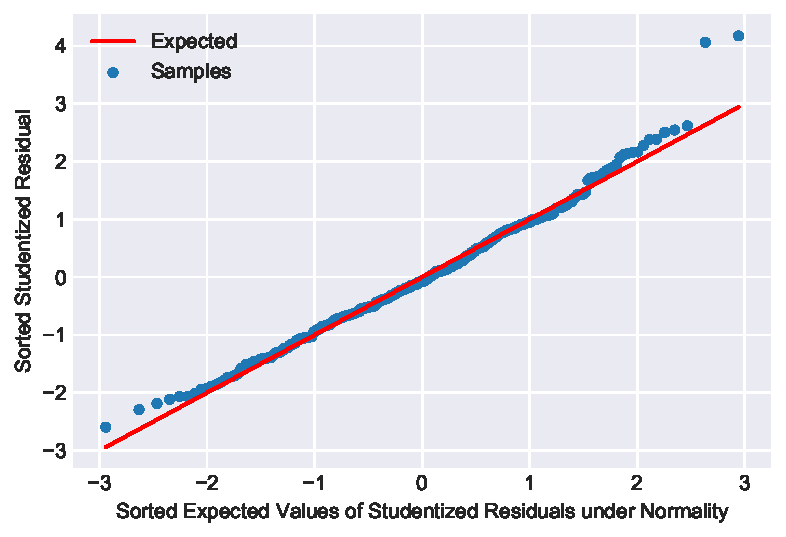
\includegraphics[width=0.8\linewidth]{img/normal_probability_plot.pdf}
  \caption[Normal probability plot to test the adequacy of the regression model]
  {Normal probability plot to test the adequacy of the regression model.}
  \label{fig:normal_probability_plot}
\end{figure}

Our samples are close to the normality which would be a straight line with a slope of 1.0. Fitting this plot, we obtain a slope of 1.001, intercept of 0.004, and the coefficient of determination $R^2$ of 0.985. The relatively high value of $R^2$ indicates that the error term $\epsilon_i$ is close to the normal distribution. Therefore, we conclude that our regression model \eqref{eqn:regression_model} is adequate. As we justified our regression model and from the hypothesis testing, we conclude that MSR does not impact the MOTA score, and QP and MSR do not depend on each other; therefore, our prediction for MSR, as explained in Section \ref{sec:background/section_e}, is inconsistent with our results. Thus, we will limit our further study to QP only.

% show the formulation
We showed that our regression model \eqref{eqn:regression_model} is appropriate and therefore, we propose to formulate the relationship between MOTA and QP. From this regression, we have the following formulations.
\begin{equation}
    \text{MOTA}' = \beta_0 + \beta_1 \cdot \text{QP}'
\end{equation}
\begin{equation}
    \text{MOTA} = \text{MOTA(Uncompressed)} - \beta_0 - \beta_1 \cdot \frac{1}{ \frac{\text{QP}}{52} - 1 }
\label{eqn:MOTA_vs_QP_formula}
\end{equation}
Substituting the estimated values of parameters from Table \ref{tab:regression}, we have the following equation.
\begin{equation}
    \text{MOTA} = 58.81 + 2.97 \cdot \frac{1}{ \frac{\text{QP}}{52} - 1 }
\label{eqn:MOTA_vs_QP_formula_substituted}
\end{equation}
We plotted the average values of MOTA measurements at each QP and overlaid the fitted model \ref{eqn:MOTA_vs_QP_formula_substituted} on the scatter plot as shown in Figure \ref{fig:MOTA_vs_QP_formulation}.
\begin{figure}[!tb]
  \centering
  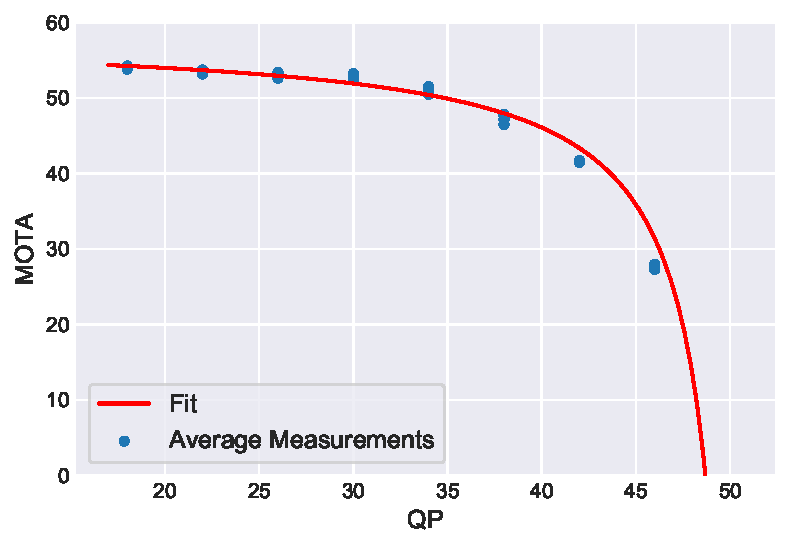
\includegraphics[width=0.8\linewidth]{img/MOTA_vs_QP_formulation.pdf}
  \caption[Scatter plot of average values of MOTA measurements and fitted model]
  {Scatter plot of average values of MOTA measurements and fitted model.}
  \label{fig:MOTA_vs_QP_formulation}
\end{figure}

Note that our model is fitted according to the raw data points for "all" object classes while average MOTA values are plotted for visualizing purposes. Also, our model is fitted based on the QP range from 18 to 46, and since QP ranges from 0 to 51 in theory \cite{sullivan_overview_2012}, our model is extrapolated. However, from the practical point of view, QP = 51 is virtually never used and the QP range from 18 to 46 is sufficient. Future study could include the whole range of QP to fit the model. In addition, not only MOTA, the same analysis procedure can be applied to all tracking metrics, and we tabulated the regression analysis results of all the metrics in Appendix \ref{sec:appendix/section_regression_all}.

% ----------------------------------------------------------
% One-sided t-test
% ----------------------------------------------------------

\subsection{One-sided t-test}
\label{subsec:/results/section_a/t_test}
Finally, to quantify the results to answer the question - at which QP, the performance score is significantly lower than the score at the uncompressed case, we conducted the one-sided t-test. As explained in Section \ref{subsec:/results/section_a/regression_analysis}, without the MOTA transformation, the variance is high. To gain the better insight with the reduced variance, we consider the difference between the score at the uncompressed case and the score at each QP. For the one-sided t-test, we included all the metrics, so we will transform each performance score as
\begin{equation}
  p_{\text{diff}} =
    \begin{cases}
         p_{\text{comp}} - p_{\text{uncomp}} ,& \text{for IDFN, FN, PT, ML} \\        
         p_{\text{uncomp}} - p_{\text{comp}} ,& \text{else} \\
    \end{cases}
\end{equation}
where $p_{\text{comp}}$ is the performance score at each QP, $p_{\text{uncomp}}$ is the the performance score at the uncompressed case, and $p_{\text{diff}}$ represents the difference of such scores. Since the scores IDFN, FN, PT, and ML increase as QP increases according to Figure \ref{fig:averaged_result_all_multiplots_qp}, we subtract $p_{\text{comp}}$ from $p_{\text{uncomp}}$. For other metrics, the scores decrease as QP increases, so we subtract $p_{\text{uncomp}}$ from $p_{\text{comp}}$. Figure \ref{fig:score_transformation} shows that after the transformation of the score, MOTA as an example, the variance is reduced at lower QP.
\begin{figure}[!tb]
  \centering
  \begin{subfigure}{.5\linewidth}
    \centering
    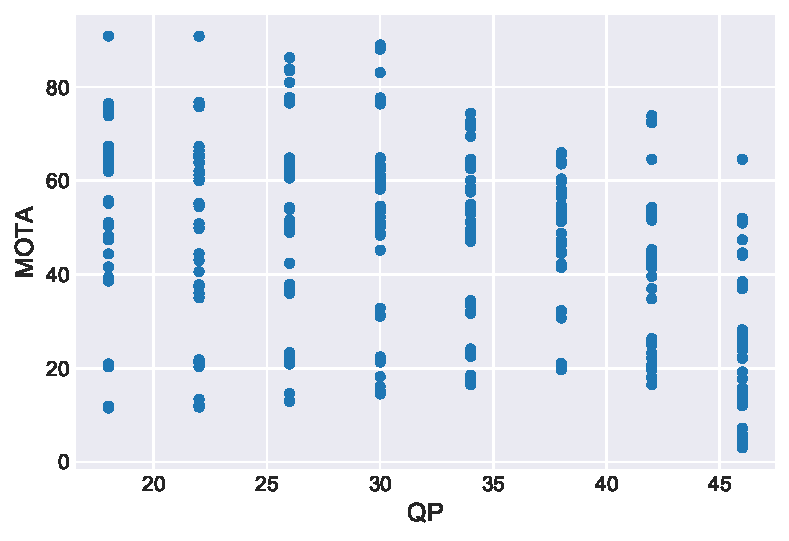
\includegraphics[width=\linewidth]{img/score_transformation_before.pdf}
    \caption{MOTA vs QP scatter plot}
    \label{fig:score_transformation_before}
  \end{subfigure}%
  \begin{subfigure}{.5\linewidth}
    \centering
    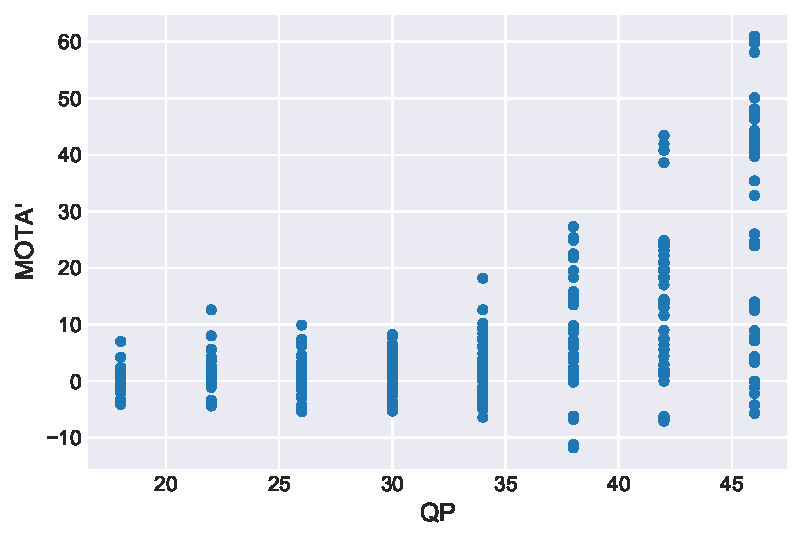
\includegraphics[width=\linewidth]{img/score_transformation_after.pdf}
    \caption{$\text{MOTA}'$ vs QP scatter plot }
    \label{fig:score_transformation_after}
  \end{subfigure}
  \caption[Scatter plots before and after the MOTA transformation for t-test]{%
    Scatter plots before and after the MOTA transformation for t-test.%
  }
  \label{fig:score_transformation}
\end{figure}

To perform t-test, the hypotheses are
\begin{equation}
    \begin{aligned}
        H_0 : \mu_{\text{diff}} \leq 0 \\
        H_1 : \mu_{\text{diff}} > 0 \\
    \end{aligned}
\end{equation}
where $\mu_{\text{diff}}$ is the mean of 12 transformed score values $p_{\text{diff}}$. The null hypothesis is the case when the mean $\mu_{\text{diff}}$ is less than or equal to the population mean of 0. The alternative hypothesis is the case when the mean $\mu_{\text{diff}}$ is greater than the population mean of 0. Applying the one-sided t-test for "all" object classes across all the video sequences at a significance level of 0.05, we obtain the results in Table \ref{tab:t_test_all} using the Python package \cite{virtanen_scipy_2020}. The value less than the significance level of 0.05 is bolded in the table.
\begin{table}[!tb]
    \centering
    \caption[One-sided t-test for "all" object classes across all the video sequences]
    {One-sided t-test for "all" object classes across all the video sequences.}
    \resizebox{1.0\linewidth}{!}{
    
% \begin{tabular}{lllllllllllllllllllll}
\begin{tabular}{ccccccccccccccccccccc}
\toprule
{} &                 IDTP &                 IDFP &                 IDFN &                 IDF1 &            IDP &                  IDR &                Recall &      Precision &                    F1 &                    MT &    PT &                   ML &                    TP &                   FP &                    FN &                  IDs &                   FM &               mAP-50 &                  MOTA &                 MOTP \\
\midrule
p-value(QP=18) &                 0.44 &                 0.90 &                 0.44 &                 0.87 &           0.70 &                 0.90 &                  0.31 &  \textbf{0.02} &                  0.06 &         \textbf{0.05} &  0.79 &        \textbf{0.02} &                  0.29 &                 0.99 &                  0.29 &                 0.98 &                 0.94 &                 0.68 &         \textbf{0.03} &                 0.97 \\
p-value(QP=22) &                 0.91 &                 0.49 &                 0.91 &                 0.79 &           0.71 &                 0.79 &   $\pmb{< |10^{-3}|}$ &  \textbf{0.03} &   $\pmb{< |10^{-2}|}$ &         \textbf{0.02} &  0.63 &        \textbf{0.03} &                  0.39 &                 0.99 &                  0.39 &                 0.92 &                 0.93 &                 0.38 &   $\pmb{< |10^{-2}|}$ &                 0.97 \\
p-value(QP=26) &                 0.16 &                 0.07 &                 0.16 &                 0.58 &           0.91 &                 0.20 &   $\pmb{< |10^{-5}|}$ &           0.89 &   $\pmb{< |10^{-3}|}$ &   $\pmb{< |10^{-3}|}$ &  0.59 &  $\pmb{< |10^{-3}|}$ &   $\pmb{< |10^{-2}|}$ &                 0.27 &   $\pmb{< |10^{-2}|}$ &                 0.53 &                 0.41 &        \textbf{0.02} &   $\pmb{< |10^{-3}|}$ &                 1.00 \\
p-value(QP=30) &                 0.08 &                 0.76 &                 0.08 &                 0.24 &           0.65 &        \textbf{0.03} &   $\pmb{< |10^{-5}|}$ &           0.83 &   $\pmb{< |10^{-2}|}$ &   $\pmb{< |10^{-3}|}$ &  0.50 &  $\pmb{< |10^{-2}|}$ &                  0.10 &                 0.84 &                  0.10 &                 0.29 &                 0.47 &                 0.08 &   $\pmb{< |10^{-3}|}$ &                 0.99 \\
p-value(QP=34) &  $\pmb{< |10^{-2}|}$ &  $\pmb{< |10^{-2}|}$ &  $\pmb{< |10^{-2}|}$ &  $\pmb{< |10^{-2}|}$ &           0.60 &  $\pmb{< |10^{-4}|}$ &   $\pmb{< |10^{-6}|}$ &           1.00 &   $\pmb{< |10^{-4}|}$ &   $\pmb{< |10^{-5}|}$ &  0.95 &  $\pmb{< |10^{-5}|}$ &   $\pmb{< |10^{-3}|}$ &        \textbf{0.01} &   $\pmb{< |10^{-3}|}$ &  $\pmb{< |10^{-3}|}$ &  $\pmb{< |10^{-2}|}$ &        \textbf{0.01} &   $\pmb{< |10^{-4}|}$ &                 0.99 \\
p-value(QP=38) &  $\pmb{< |10^{-3}|}$ &  $\pmb{< |10^{-6}|}$ &  $\pmb{< |10^{-3}|}$ &  $\pmb{< |10^{-4}|}$ &           0.88 &  $\pmb{< |10^{-6}|}$ &   $\pmb{< |10^{-7}|}$ &           1.00 &   $\pmb{< |10^{-6}|}$ &   $\pmb{< |10^{-7}|}$ &  0.92 &  $\pmb{< |10^{-7}|}$ &   $\pmb{< |10^{-4}|}$ &  $\pmb{< |10^{-4}|}$ &   $\pmb{< |10^{-4}|}$ &  $\pmb{< |10^{-2}|}$ &  $\pmb{< |10^{-2}|}$ &  $\pmb{< |10^{-3}|}$ &   $\pmb{< |10^{-5}|}$ &                 0.57 \\
p-value(QP=42) &  $\pmb{< |10^{-5}|}$ &  $\pmb{< |10^{-4}|}$ &  $\pmb{< |10^{-5}|}$ &  $\pmb{< |10^{-6}|}$ &           0.17 &  $\pmb{< |10^{-7}|}$ &  $\pmb{< |10^{-10}|}$ &           1.00 &   $\pmb{< |10^{-8}|}$ &   $\pmb{< |10^{-9}|}$ &  0.40 &  $\pmb{< |10^{-6}|}$ &   $\pmb{< |10^{-8}|}$ &  $\pmb{< |10^{-5}|}$ &   $\pmb{< |10^{-8}|}$ &  $\pmb{< |10^{-3}|}$ &                 0.12 &  $\pmb{< |10^{-5}|}$ &   $\pmb{< |10^{-8}|}$ &        \textbf{0.01} \\
p-value(QP=46) &  $\pmb{< |10^{-8}|}$ &  $\pmb{< |10^{-4}|}$ &  $\pmb{< |10^{-8}|}$ &  $\pmb{< |10^{-9}|}$ &  \textbf{0.04} &  $\pmb{< |10^{-9}|}$ &  $\pmb{< |10^{-13}|}$ &           0.23 &  $\pmb{< |10^{-12}|}$ &  $\pmb{< |10^{-13}|}$ &  0.69 &  $\pmb{< |10^{-8}|}$ &  $\pmb{< |10^{-11}|}$ &        \textbf{0.02} &  $\pmb{< |10^{-11}|}$ &  $\pmb{< |10^{-2}|}$ &        \textbf{0.01} &  $\pmb{< |10^{-9}|}$ &  $\pmb{< |10^{-11}|}$ &  $\pmb{< |10^{-3}|}$ \\
\bottomrule
\end{tabular}

    }
\label{tab:t_test_all}
\end{table}
From this result, for example, the MOTA score at QP = 18 is significantly lower than the score of the uncompressed sequence with 95\% confidence as we reject the null hypothesis. In fact, we can conclude for most of the metrics except Precision and PT as following; the performance score is greater than the uncompressed score for the metrics IDFN, FN, and ML but the performance score is less than the uncompressed score for other metrics at specific QP with 95\% confidence. From Figure \ref{fig:averaged_result_all_multiplots_qp}, the Precision score increases first and then decreases as QP increases. Therefore, the result from the one-sided t-test is consistent with the the visualization. According to Equation \ref{eqn:Precision}, Precision depends on TP and FP, and the increase of p-value in FP can be confirmed at QP = 30. The detailed reasoning for this outcome is explained in the following Section \ref{sec:results/section_b}. A slight increase of MOTP can also be confirmed from QP = 26. We also applied the one-sided t-test to the "person" object class and similar conclusions can be made. See Appendix \ref{sec:appendix/section_t_test_0} for the "person" object case.

As we just showed the results from the visualization and the statistical analysis for the multiple video sequences, most metrics behave in a way as expected, but the outcomes of Precision and MOTP were not entirely expected. We will further analyze individual sequences in the next section.


% As \cite{sharrab_modeling_2017} shows that bitrate is inversely proportional to QP and HEVC range from 0 to 51 \cite{sullivan_overview_2012}, our proposed formula 

\section{Case Study of Individual Sequences}
\label{sec:results/section_b}

In this section, we will look into the individual sequences to support the averaged result obtained in the earlier section. Out of 12 video samples, we observed the two categories of different results as we named Category I and Category II. For the first category, the result is consistent with the hypothesis on different QP such that most performance scores decrease as QP increases while showing the lower performances than the uncompressed sequences. However, for the second category, the performance scores increase but starts decreasing at high QP, and the performance for the compressed sequences outperform the uncompressed ones before the high QP. We observed that the first category of result is observed in most of the video sequences except Class B Cactus, Class D BlowingBubbles, Class E FourPeople, and Class E KristenAndSara which are observed in the other category. We will examine the Class D BasketballPass, Class E Johnny, Class D BlowingBubbles, Class B Cactus as cases studies. Instead of tracking all of the object classes, we limit the tracking on the Person class to analyze the difference between the two categories. The Person class is "cleaner" in result than other classes because the Person object class is more continuously present across the frames while other object classes such as Sports ball and Handbag are more discontinuous in frames. Not only Person class, we included the Potted plant object class in Class B Cactus.


\subsection{Class D BasketballPass}
We examined the result from the individual video sequence of Class D BasketballPass. This sequence consists of 7 Person objects and the occlusion occurs frequently in the video.  Figure \ref{fig:BasketballPass_0_multiplots_qp} shows all the performance score on different QP at MSR = 16 from the video and Table \ref{tab:BasketballPass_0} shows each numerical value. We selected MSR = 16 out of different MSR values since different MSR did not make a significant difference from the regression analysis in the previous section.
\begin{figure}[!htbp]
  \centering
  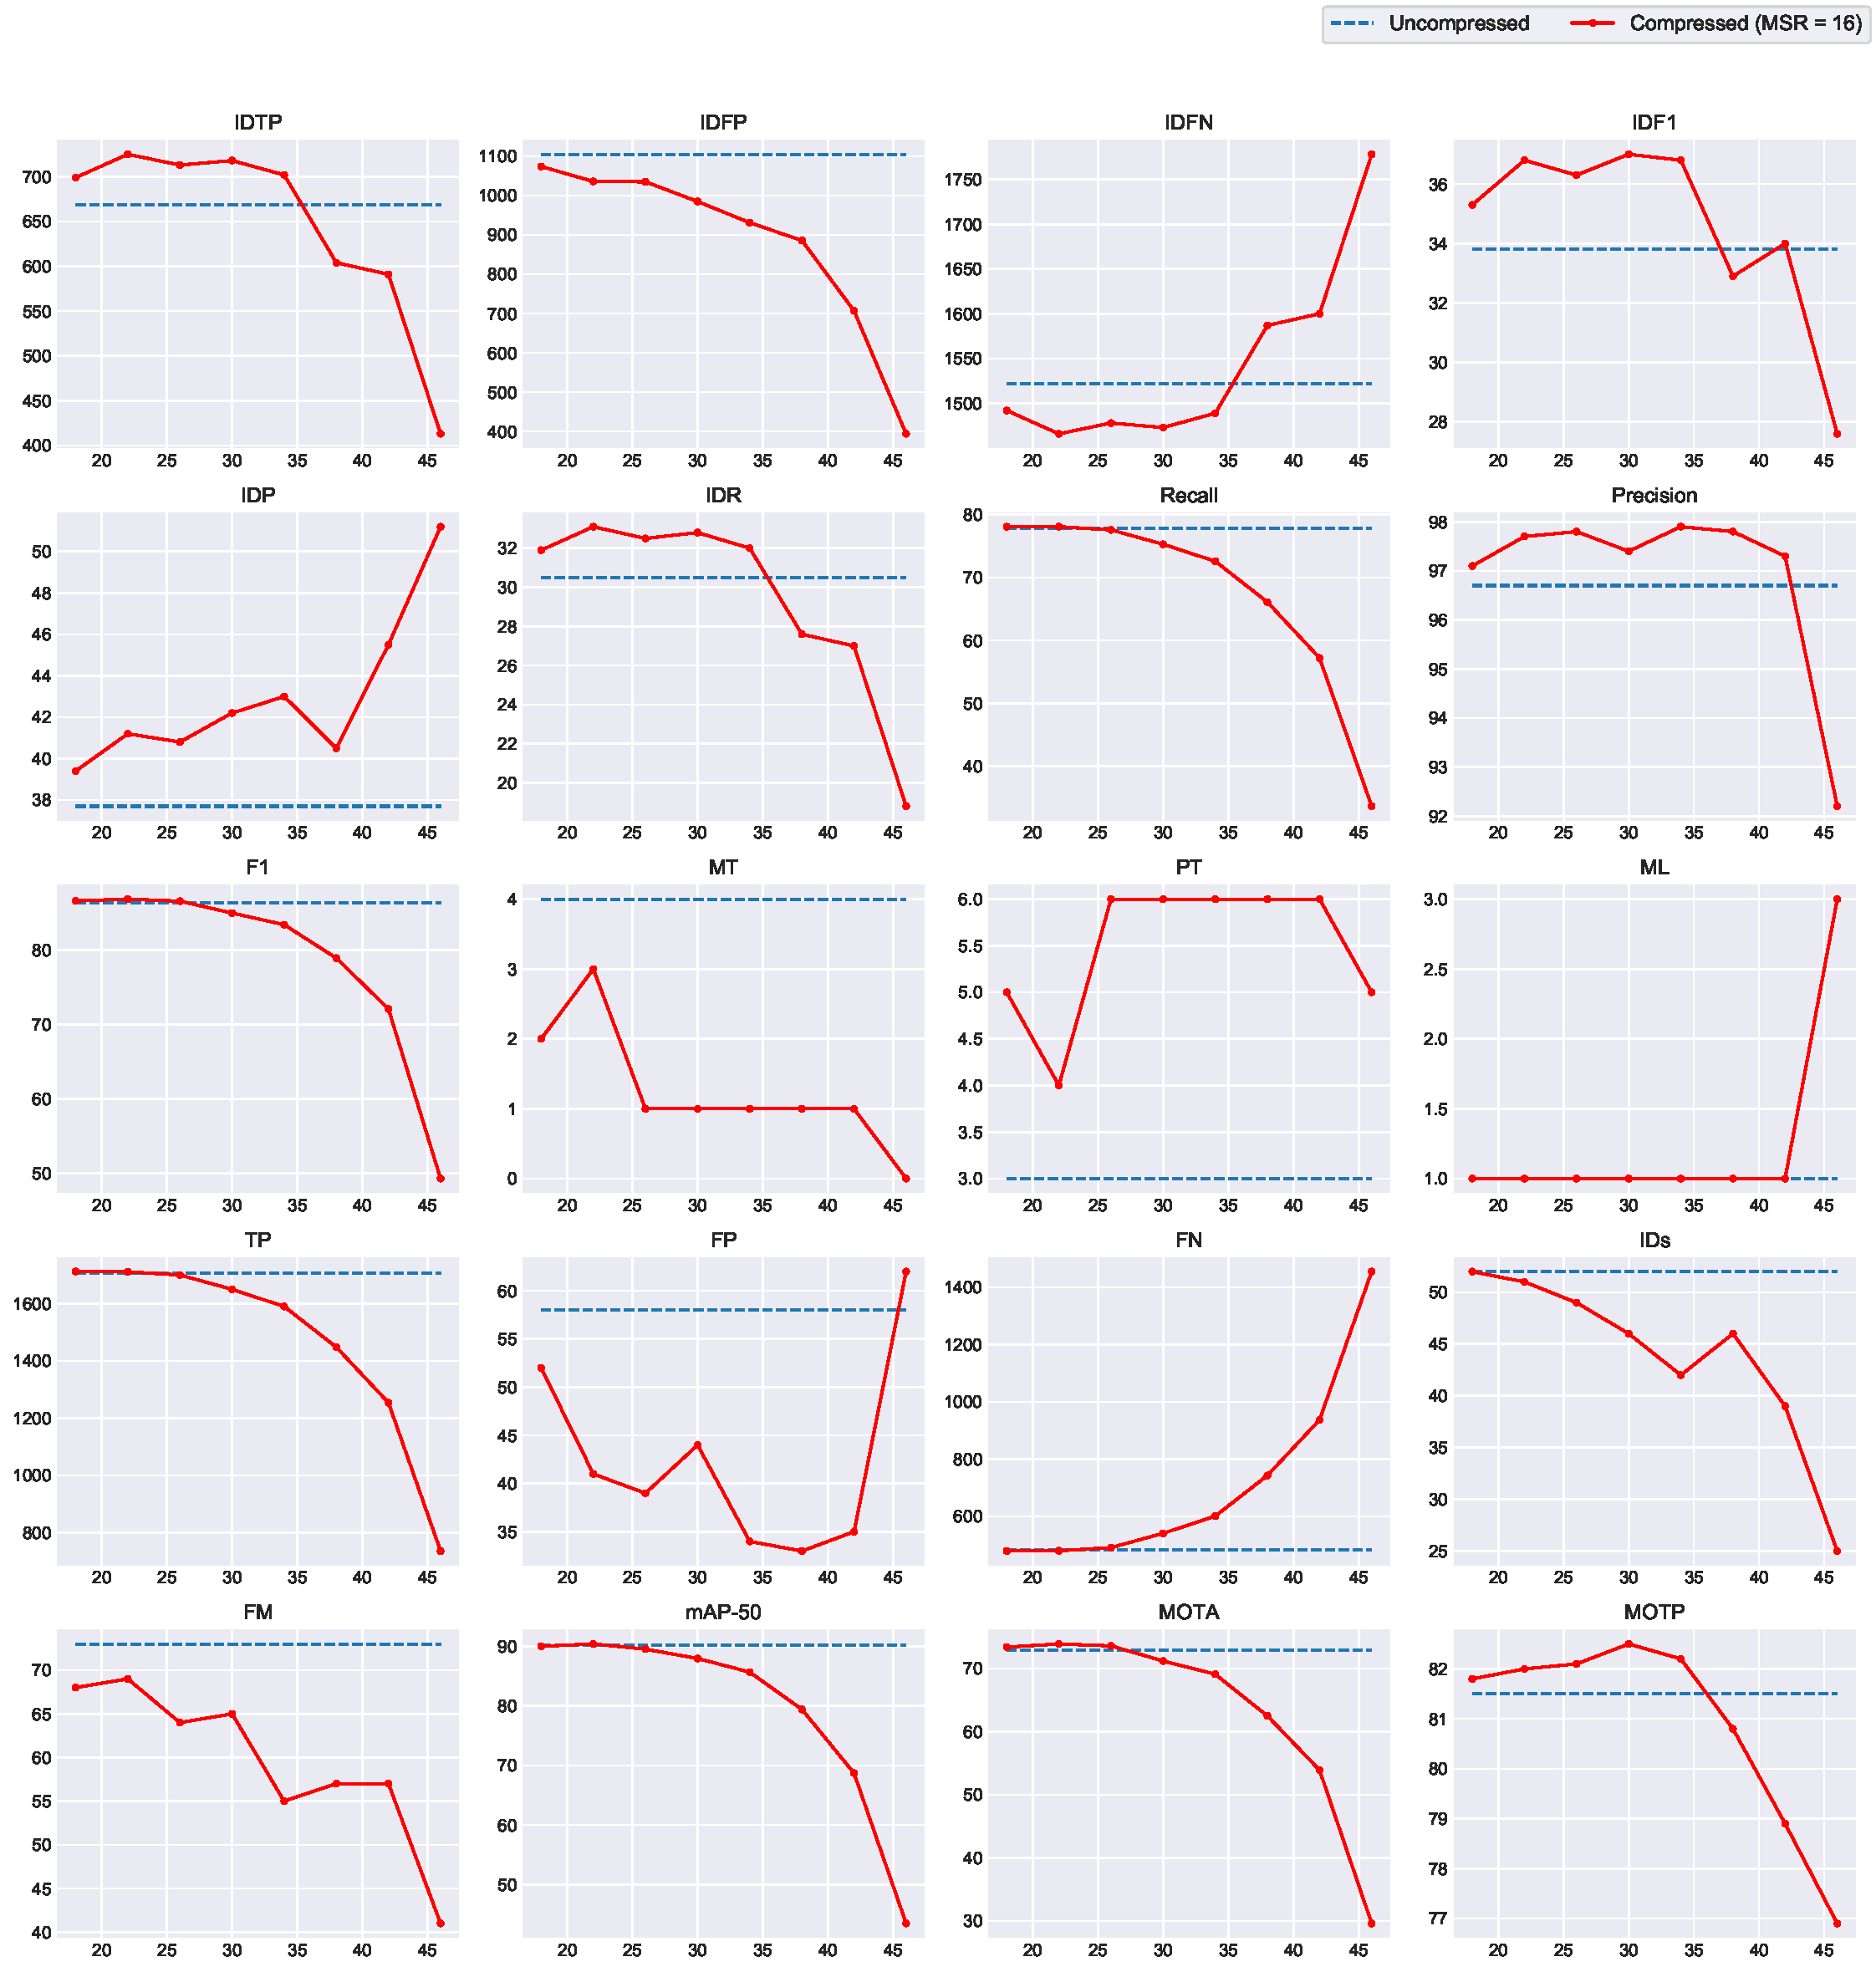
\includegraphics[width=1.0\linewidth]{img/BasketballPass_0_multiplots_qp.pdf}
  \caption[Visualization of the performance results in Class D BasketballPass at different QP for the "person" object class]
  {Visualization of the performance results in Class D BasketballPass at different QP for the "person" object class.
  }
  \label{fig:BasketballPass_0_multiplots_qp}
\end{figure}
\begin{table}[!tb]
    \centering
    \caption[Performance results on BasketballPass]
    {Performance results on BasketballPass.}
    \resizebox{1.0\linewidth}{!}{
\begin{tabular}{llrrrrrrrrrrrrrrrrrrrrr}
\toprule
          QP &          MSR &   IDTP &    IDFP &    IDFN &  IDF1 &   IDP &   IDR &  Recall &  Precision &    F1 &  GT &  MT &  PT &  ML &   TP &  FP &   FN &  IDs &  FM &  mAP-50 &  MOTA &  MOTP \\
\midrule
Uncompressed & Uncompressed & 669.00 & 1105.00 & 1522.00 & 33.80 & 37.70 & 30.50 &   77.90 &      96.70 & 86.29 &   8 &   4 &   3 &   1 & 1707 &  58 &  484 &   52 &  73 &   90.25 & 72.90 & 81.50 \\
          18 &           16 & 699.00 & 1074.00 & 1492.00 & 35.30 & 39.40 & 31.90 &   78.10 &      97.10 & 86.57 &   8 &   2 &   5 &   1 & 1712 &  52 &  479 &   52 &  68 &   90.03 & 73.40 & 81.80 \\
          22 &           16 & 725.00 & 1036.00 & 1466.00 & 36.80 & 41.20 & 33.10 &   78.10 &      97.70 & 86.81 &   8 &   3 &   4 &   1 & 1711 &  41 &  480 &   51 &  69 &   90.42 & 73.90 & 82.00 \\
          26 &           16 & 713.00 & 1035.00 & 1478.00 & 36.30 & 40.80 & 32.50 &   77.60 &      97.80 & 86.54 &   8 &   1 &   6 &   1 & 1700 &  39 &  491 &   49 &  64 &   89.54 & 73.60 & 82.10 \\
          30 &           16 & 718.00 &  985.00 & 1473.00 & 37.00 & 42.20 & 32.80 &   75.30 &      97.40 & 84.94 &   8 &   1 &   6 &   1 & 1650 &  44 &  541 &   46 &  65 &   87.98 & 71.20 & 82.50 \\
          34 &           16 & 702.00 &  931.00 & 1489.00 & 36.80 & 43.00 & 32.00 &   72.60 &      97.90 & 83.37 &   8 &   1 &   6 &   1 & 1590 &  34 &  601 &   42 &  55 &   85.69 & 69.10 & 82.20 \\
          38 &           16 & 604.00 &  886.00 & 1587.00 & 32.90 & 40.50 & 27.60 &   66.10 &      97.80 & 78.88 &   8 &   1 &   6 &   1 & 1448 &  33 &  743 &   46 &  57 &   79.42 & 62.50 & 80.80 \\
          42 &           16 & 591.00 &  707.00 & 1600.00 & 34.00 & 45.50 & 27.00 &   57.20 &      97.30 & 72.05 &   8 &   1 &   6 &   1 & 1254 &  35 &  937 &   39 &  57 &   68.72 & 53.90 & 78.90 \\
          46 &           16 & 413.00 &  394.00 & 1778.00 & 27.60 & 51.20 & 18.80 &   33.60 &      92.20 & 49.25 &   8 &   0 &   5 &   3 &  736 &  62 & 1455 &   25 &  41 &   43.45 & 29.60 & 76.90 \\
\bottomrule
\end{tabular}
    }
    \label{tab:BasketballPass_0}
\end{table}
The result is consistent with the averaged result shown in Chapter \ref{sec:results/section_a} such that the performance decreases as QP increases on most of the metrics except IDP and MOTP. To examine the result more thoroughly, we inspected the video sequence in frame by frame at different QP.
\begin{figure}[!tb]
  \centering
  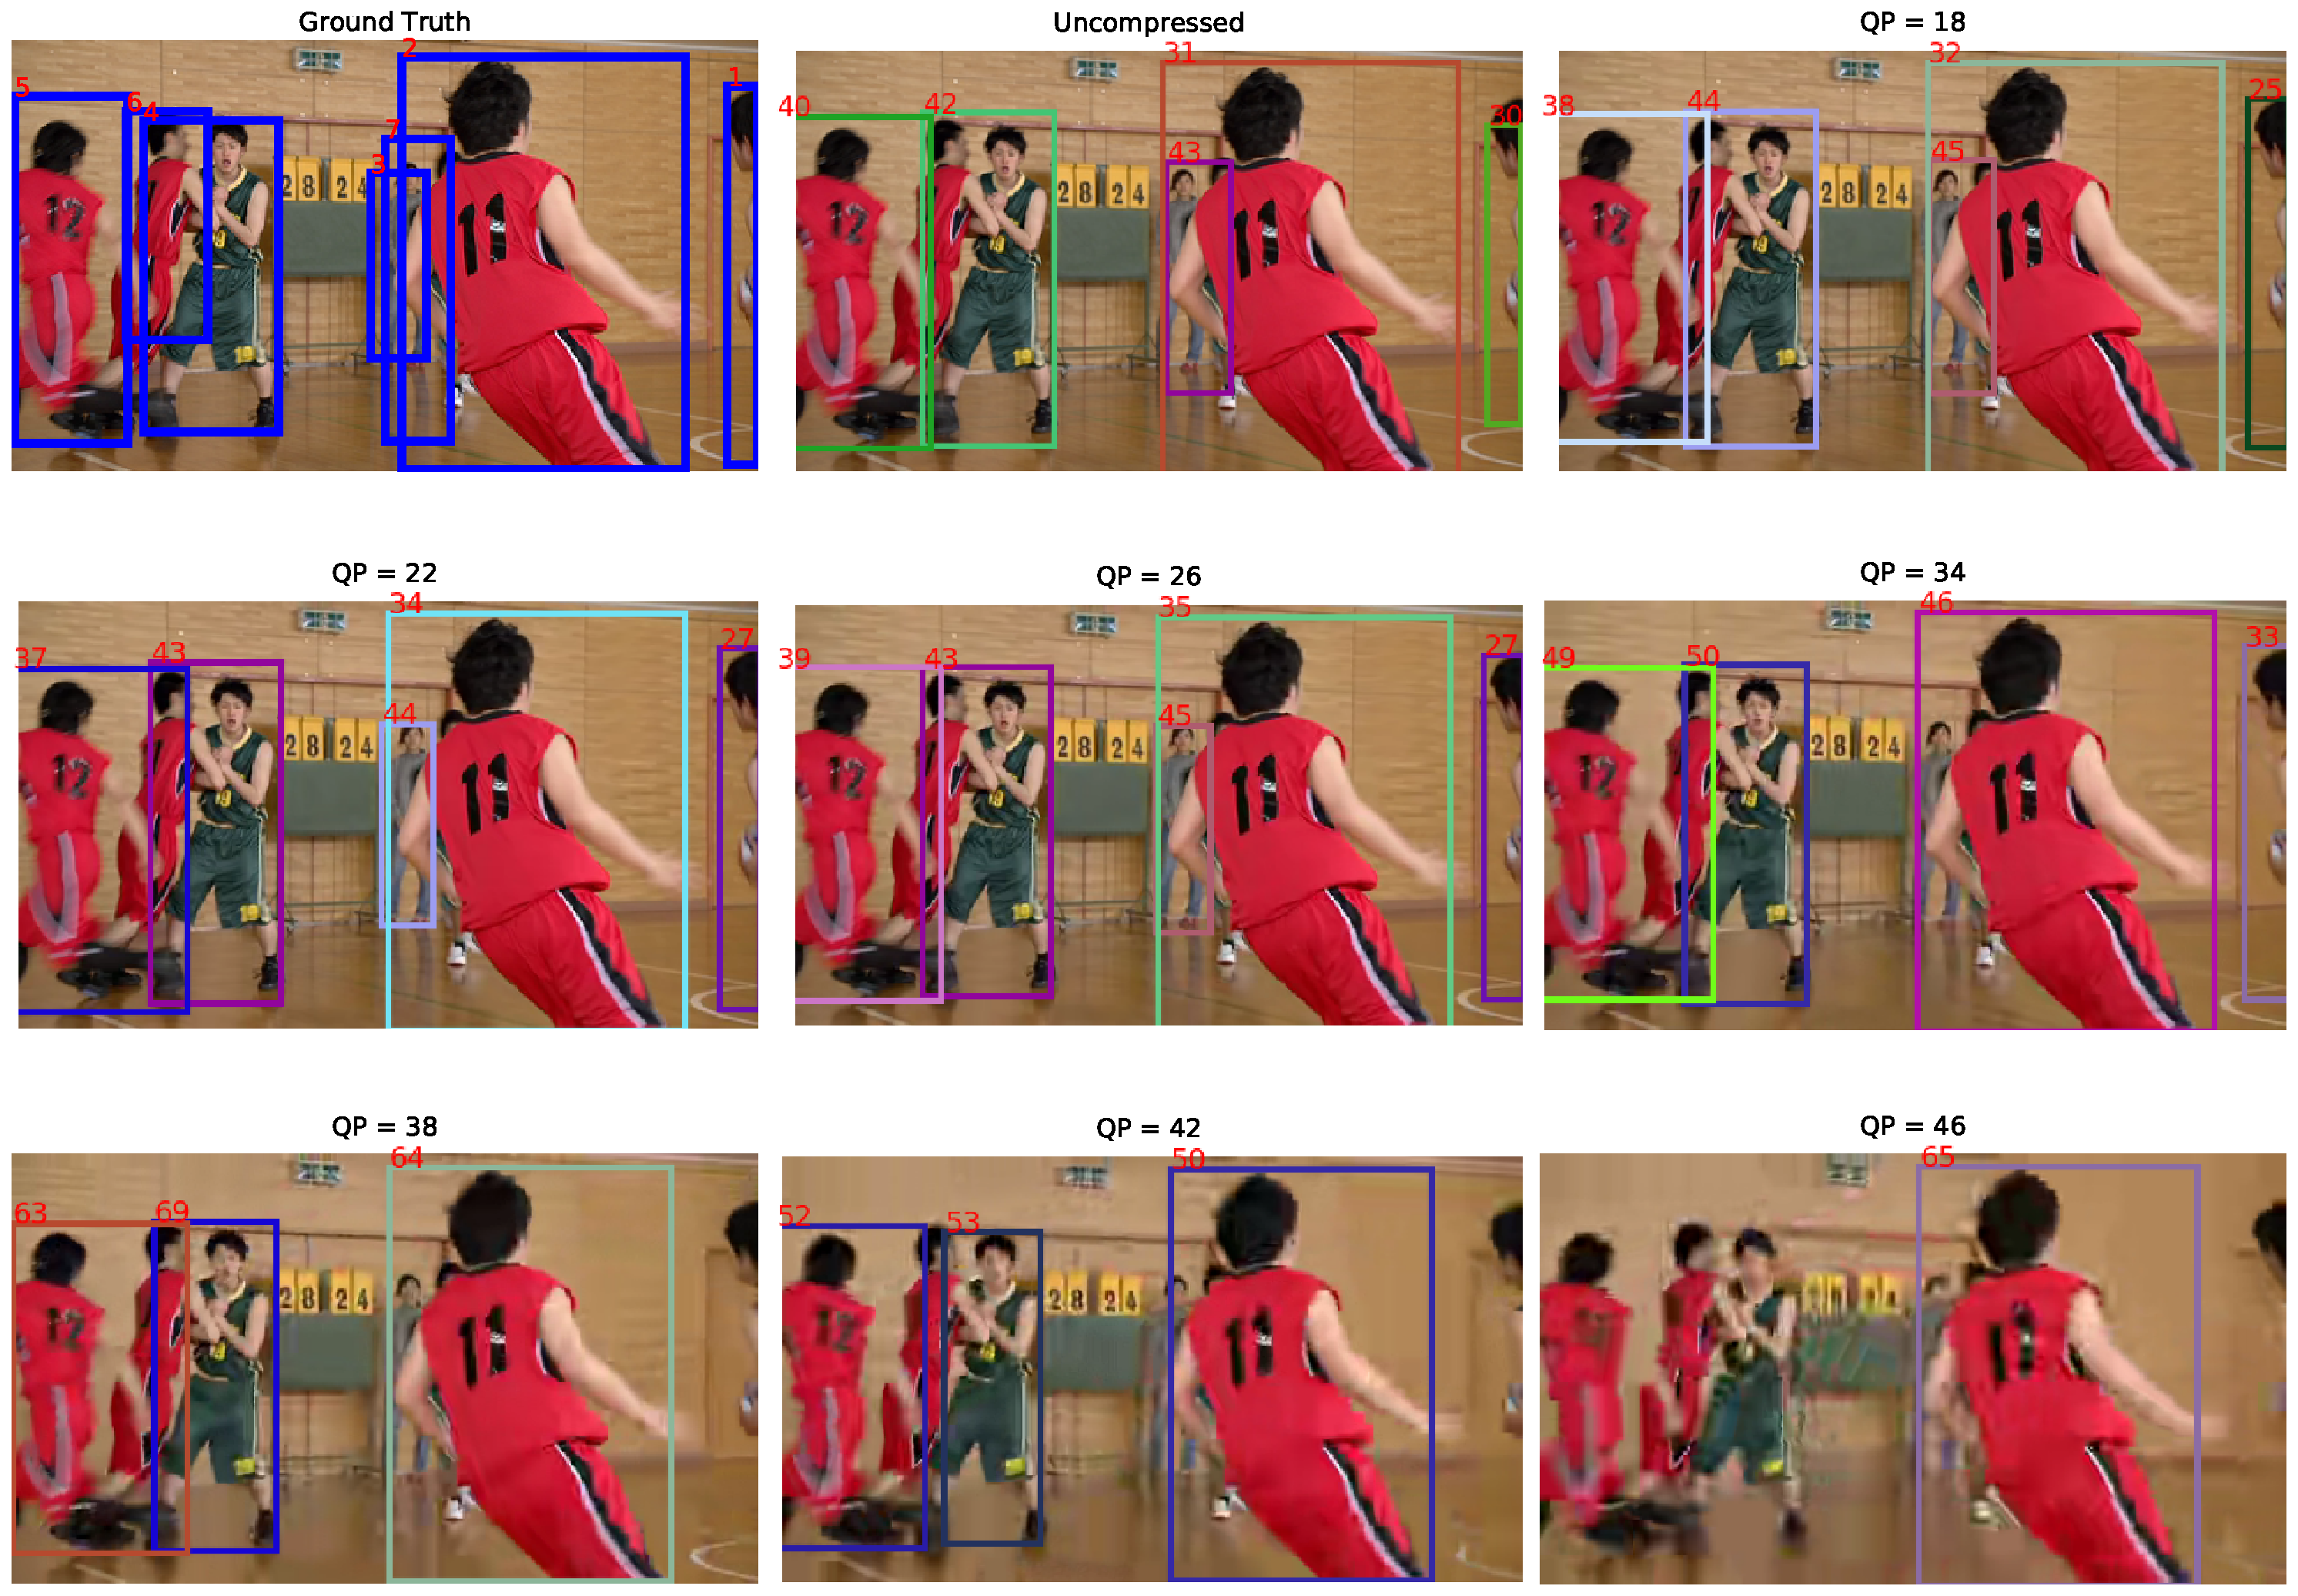
\includegraphics[width=1.0\linewidth]{img/BasketballPass_0_frame320.pdf}
  \caption[Comparison of ground truth and tracking results on the BasketballPass sequence in frames 320 at different QP]
  {
  Comparison of ground truth and tracking results on the BasketballPass sequence in frames at 320 at different QP.
  }
  \label{fig:BasketballPass_0_frame320}
\end{figure}
The figure \ref{fig:BasketballPass_0_frame320} shows comparison of ground truth, tracking results without compression, and with compression at different QP in the Class D BasketballPass sequence at frame 320. This comparison reveals that the higher the QP, the image quality decreases. As the quality decreases, the YOLOv3 detector starts failing to detect the Person objects, and hence we confirmed that FN increases. We also confirmed that IDs decreases because the number of detected objects decreases, therefore the number of times the objects being occluded decreases. When occlusions decreases, ID switch on the trajectories should decrease. For the FP, we were not able to observe and conclude the reasoning why FP increases at high QP from the Class D BasketballPass sequence alone. From FN, FP, and IDs, the increase of FN is significantly larger than the decrease of IDs and FP, so we concluded that MOTA will decrease as QP increases based on the equation \ref{eqn:MOTA}. From the Figure \ref{fig:BasketballPass_0_multiplots_qp}, we observed that IDP increases. As we confirmed that the number of occlusions decreases as QP increases, we can verify that IDFP will decrease. Hence, based on the IDP equation \ref{eqn:IDP}, due to the drop of IDFP, IDP increases. This result can also be explained qualitatively that as QP increases, occlusions occurs less, so the incorrect ID assignments occurs less, which makes ID precision higher at a higher QP. For the MOTP, we were are not able to conclude the reasoning of the increase of MOTP up to QP = 30.

\subsection{Class E Johnny}
Class E Johnny sequence consists of 9 Person objects. The occlusion was not observed, and the objects scarcely move. Figure \ref{fig:Johnny_0_multiplots_qp} shows the visualization of all the performance metrics at different QP, and Table \ref{tab:Johnny_0} shows the corresponding numerical values. 
\begin{figure}[!tb]
  \centering
  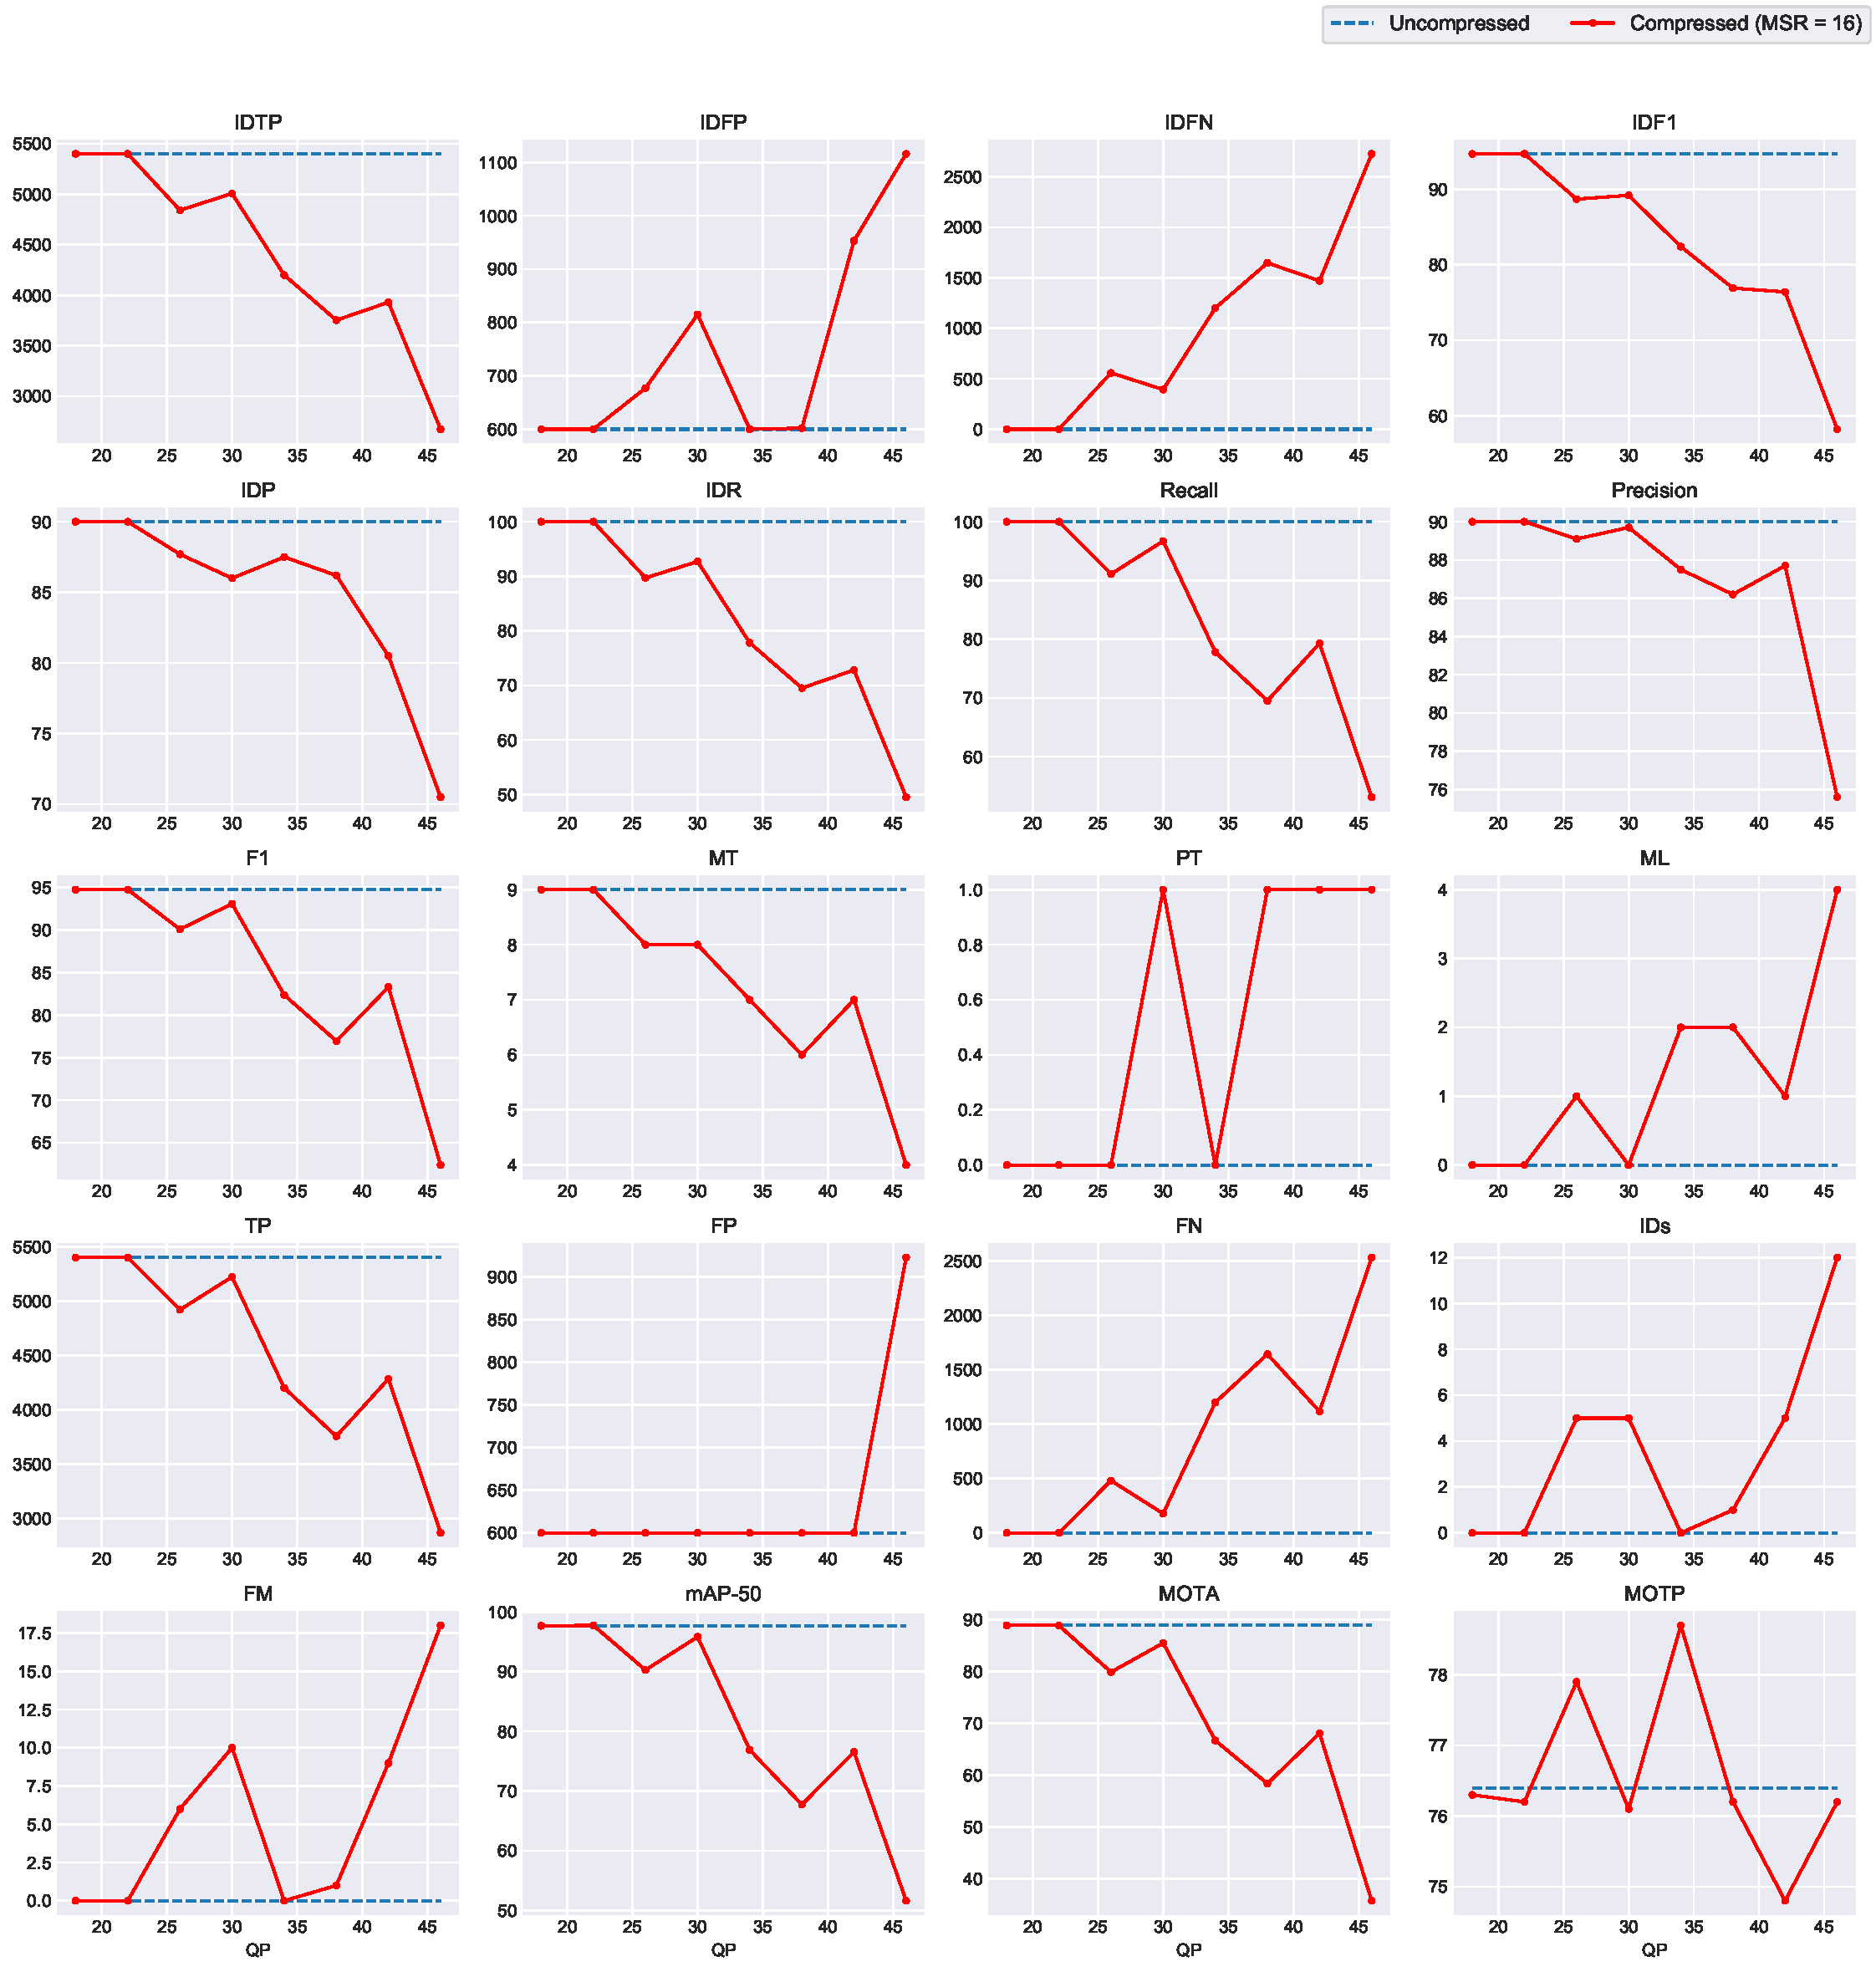
\includegraphics[width=1.0\linewidth]{img/Johnny_0_multiplots_qp.pdf}
  \caption[Visualization of the performance results on Johnny at different QP for the "person" object class]
  {
  Visualization of the performance results on Johnny at different QP for the "person" object class.
  }
  \label{fig:Johnny_0_multiplots_qp}
\end{figure}
\begin{table}[!tb]
    \centering
    \caption[Performance results on Johnny]
    {Performance results on Johnny.}
    \resizebox{1.0\linewidth}{!}{
\begin{tabular}{llrrrrrrrrrrrrrrrrrrrrr}
\toprule
          QP &          MSR &    IDTP &    IDFP &    IDFN &  IDF1 &   IDP &    IDR &  Recall &  Precision &    F1 &  GT &  MT &  PT &  ML &   TP &  FP &   FN &  IDs &  FM &  mAP-50 &  MOTA &  MOTP \\
\midrule
Uncompressed & Uncompressed & 5400.00 &  600.00 &    0.00 & 94.70 & 90.00 & 100.00 &  100.00 &      90.00 & 94.74 &   9 &   9 &   0 &   0 & 5400 & 600 &    0 &    0 &   0 &   97.72 & 88.90 & 76.40 \\
          18 &           16 & 5400.00 &  600.00 &    0.00 & 94.70 & 90.00 & 100.00 &  100.00 &      90.00 & 94.74 &   9 &   9 &   0 &   0 & 5400 & 600 &    0 &    0 &   0 &   97.70 & 88.90 & 76.30 \\
          22 &           16 & 5400.00 &  600.00 &    0.00 & 94.70 & 90.00 & 100.00 &  100.00 &      90.00 & 94.74 &   9 &   9 &   0 &   0 & 5400 & 600 &    0 &    0 &   0 &   97.76 & 88.90 & 76.20 \\
          26 &           16 & 4842.00 &  677.00 &  558.00 & 88.70 & 87.70 &  89.70 &   91.10 &      89.10 & 90.09 &   9 &   8 &   0 &   1 & 4919 & 600 &  481 &    5 &   6 &   90.29 & 79.90 & 77.90 \\
          30 &           16 & 5007.00 &  815.00 &  393.00 & 89.20 & 86.00 &  92.70 &   96.70 &      89.70 & 93.07 &   9 &   8 &   1 &   0 & 5222 & 600 &  178 &    5 &  10 &   95.85 & 85.50 & 76.10 \\
          34 &           16 & 4200.00 &  600.00 & 1200.00 & 82.40 & 87.50 &  77.80 &   77.80 &      87.50 & 82.37 &   9 &   7 &   0 &   2 & 4200 & 600 & 1200 &    0 &   0 &   76.89 & 66.70 & 78.70 \\
          38 &           16 & 3753.00 &  602.00 & 1647.00 & 76.90 & 86.20 &  69.50 &   69.50 &      86.20 & 76.95 &   9 &   6 &   1 &   2 & 3755 & 600 & 1645 &    1 &   1 &   67.73 & 58.40 & 76.20 \\
          42 &           16 & 3930.00 &  953.00 & 1470.00 & 76.40 & 80.50 &  72.80 &   79.30 &      87.70 & 83.29 &   9 &   7 &   1 &   1 & 4283 & 600 & 1117 &    5 &   9 &   76.54 & 68.10 & 74.80 \\
          46 &           16 & 2673.00 & 1116.00 & 2727.00 & 58.20 & 70.50 &  49.50 &   53.10 &      75.60 & 62.38 &   9 &   4 &   1 &   4 & 2866 & 923 & 2534 &   12 &  18 &   51.60 & 35.80 & 76.20 \\
\bottomrule
\end{tabular}
    }
    \label{tab:Johnny_0}
\end{table}
This result reveals that the most performance metrics decrease as QP increases similar to the case from the Class D BasketballPass. The decrease of performance can be verified from the Figure \ref{fig:Johnny_0_frame400} such that the objects are starting to not be detected.
\begin{figure}[!htbp]
  \centering
  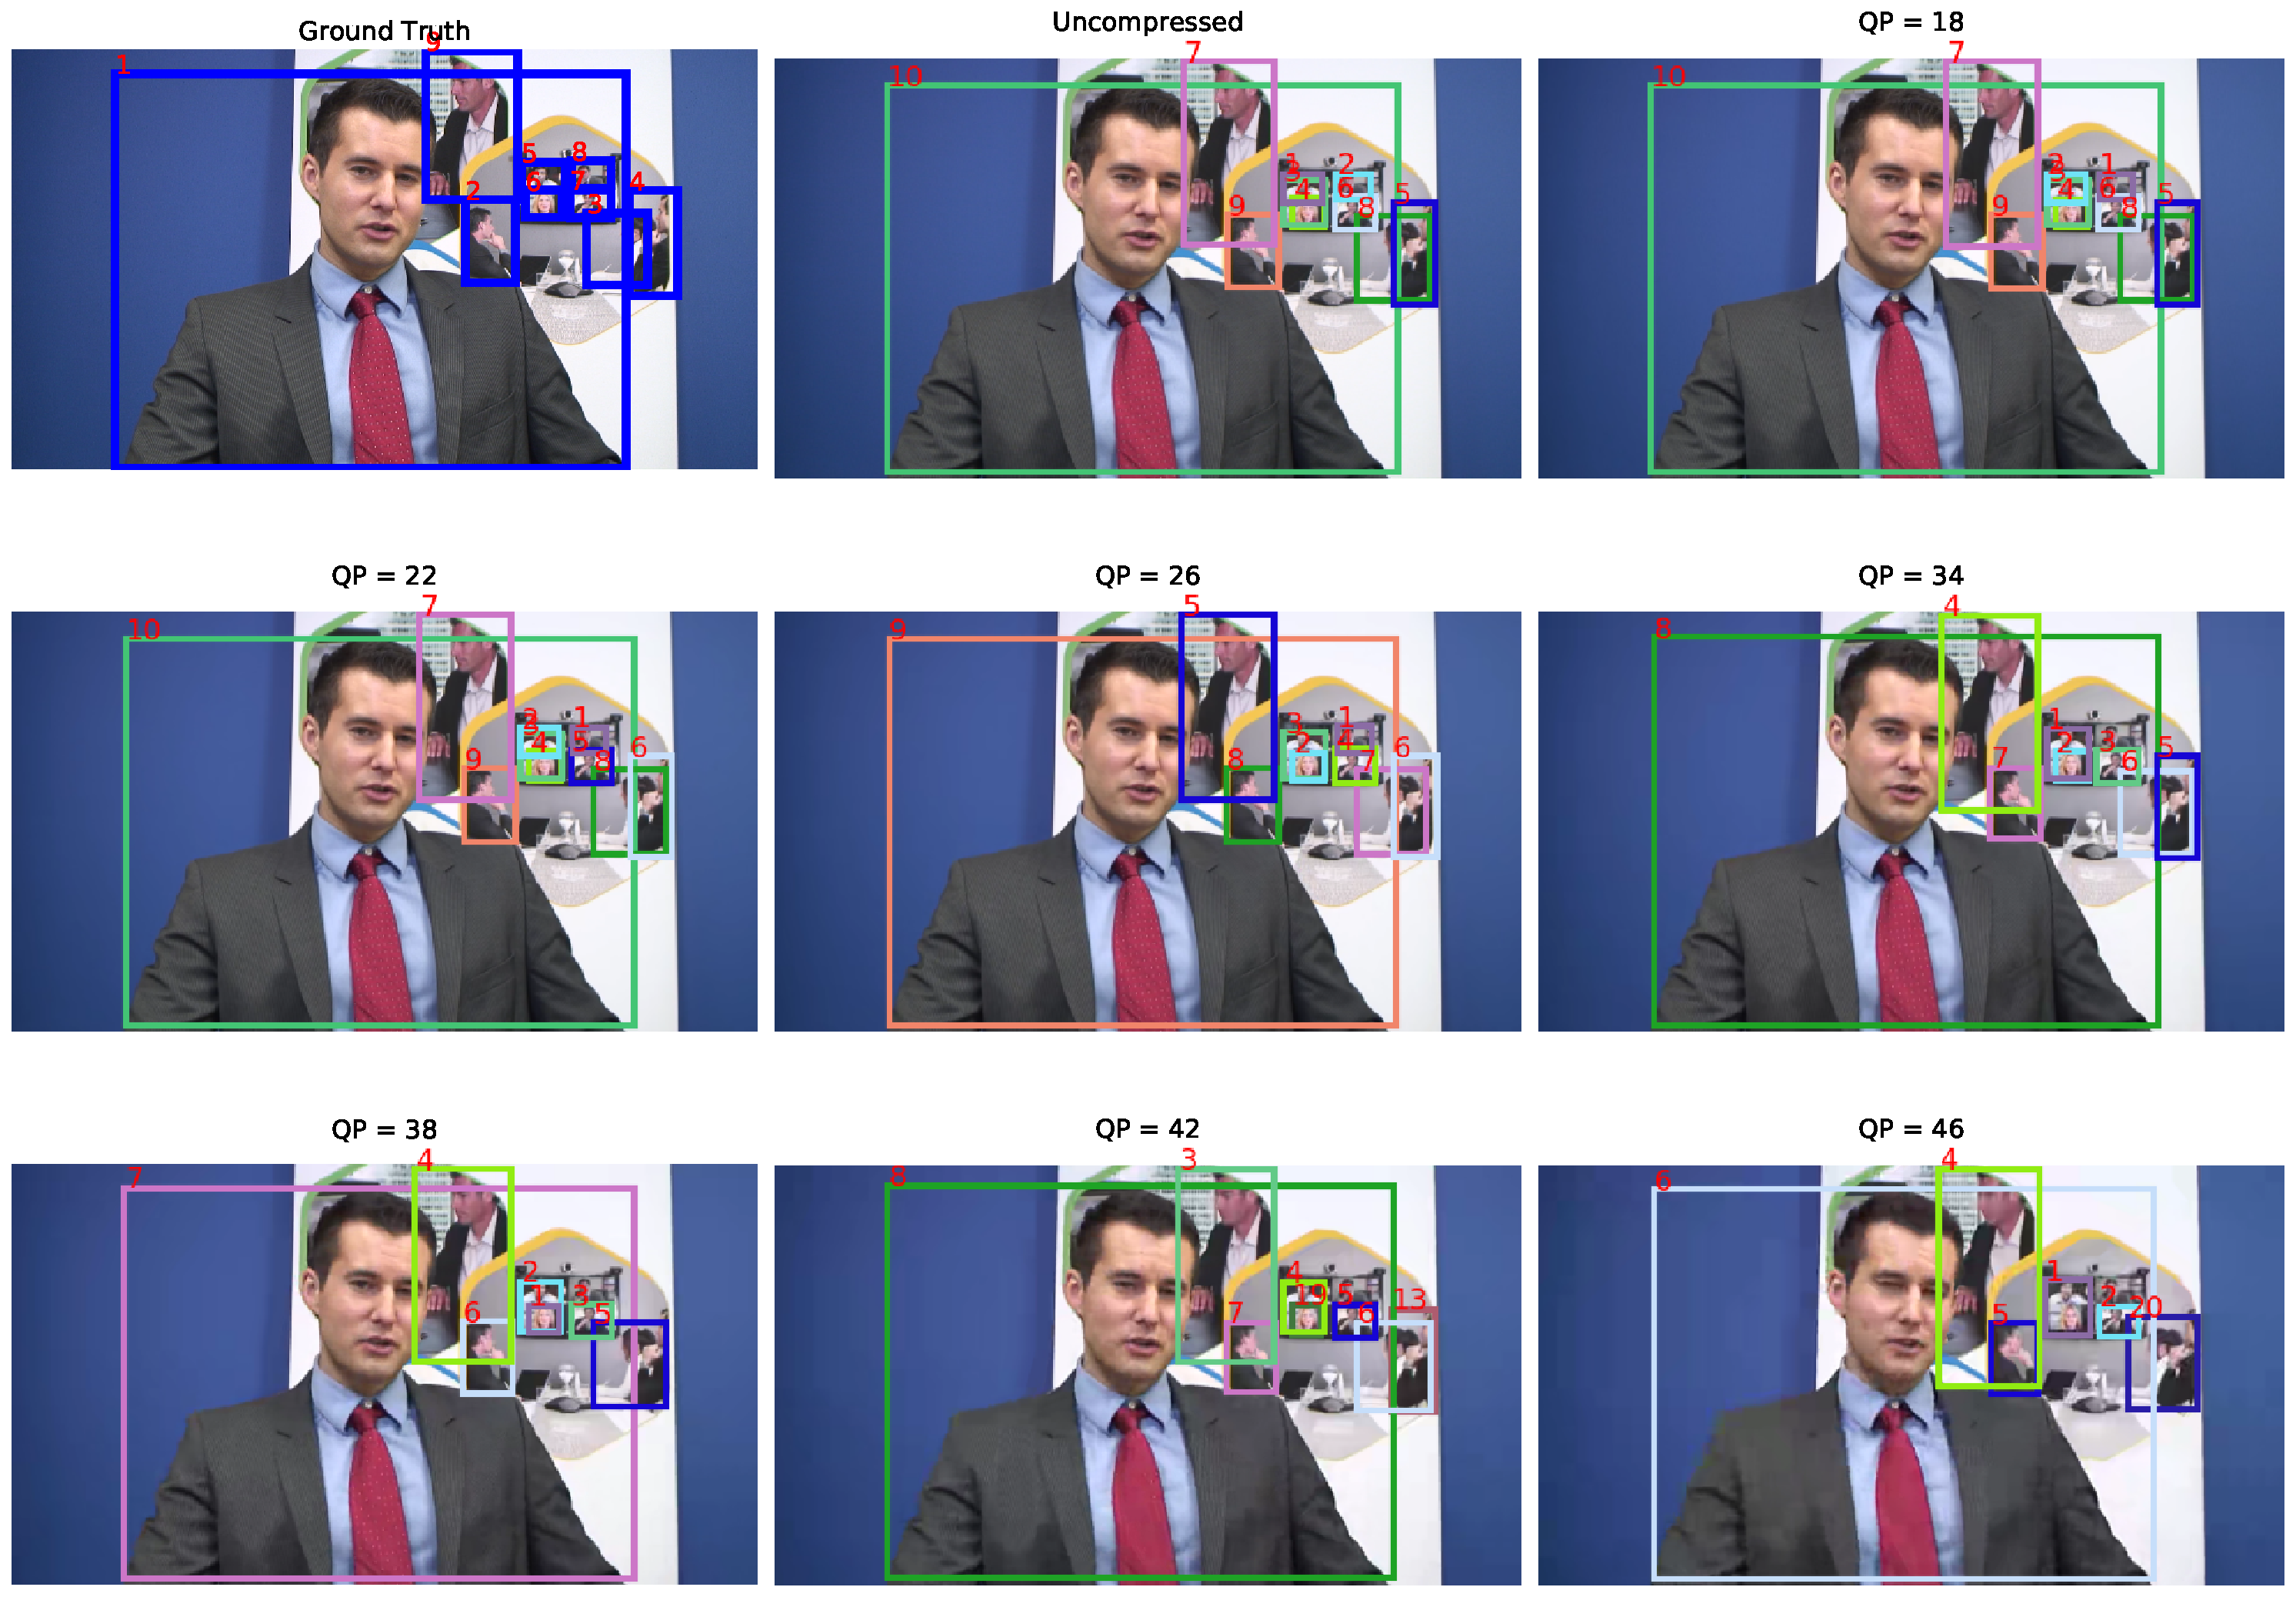
\includegraphics[width=1.0\linewidth]{img/Johnny_0_frame400.pdf}
  \caption[Comparison of Class E Johnny image frames at 320 at different QP]
  {
  Comparison of Class E Johnny image frames at 320 at different QP
  }
  \label{fig:Johnny_0_frame400}
\end{figure}
The decrease of detections proves the increase of FN. ID switch did not occur in the uncompressed sequence but was observed in the higher QP in the video sequence. Therefore, there is an increase of IDs at the higher QP. The increase of IDs can be explained qualitatively that since there is no occlusion in this sequence, ID switch between the trajectories does not occur at the lower QP but starts to occur at the high QP as the image quality drops and the detector detects the wrong target, leading to the ID switch. Based on all the increase of FP, FN, IDs, the general tracking performance metric of MOTA decreases as QP increases. Note that occlusion does not necessary correlate with the number of IDs since IDs is counted whenever a different identity is assigned to the target after re-identification (re-ID). In this sequence, the image quality drops and the detection becomes more discontinuous and re-ID is attempted but different ID is assigned to the target, thereby IDs increases as QP increases. Since IDs increases, we expect IDP to decrease. This is because the more ID switch to occur, we expect the ID precision to be lower and indeed IDR also decreases. Therefore, we confirmed that ID performance drops as QP increases. We also observed that other metrics such as detection performance and track quality drops as QP increases. The result in this sequence is different from the result of Class D BasketballPass such that the occlusion does not occur and hence ID precision decreases as image quality drops. 

\subsection{Class D BlowingBubbles}
We will now examine the sequence where we observed a decrease of general tracking performance of MOTA, which can be confirmed in the visualization from Figure \ref{fig:BlowingBubbles_0_multiplots_qp} and the numerical values from Table \ref{tab:BlowingBubbles_0}.
\begin{figure}[!tb]
  \centering
  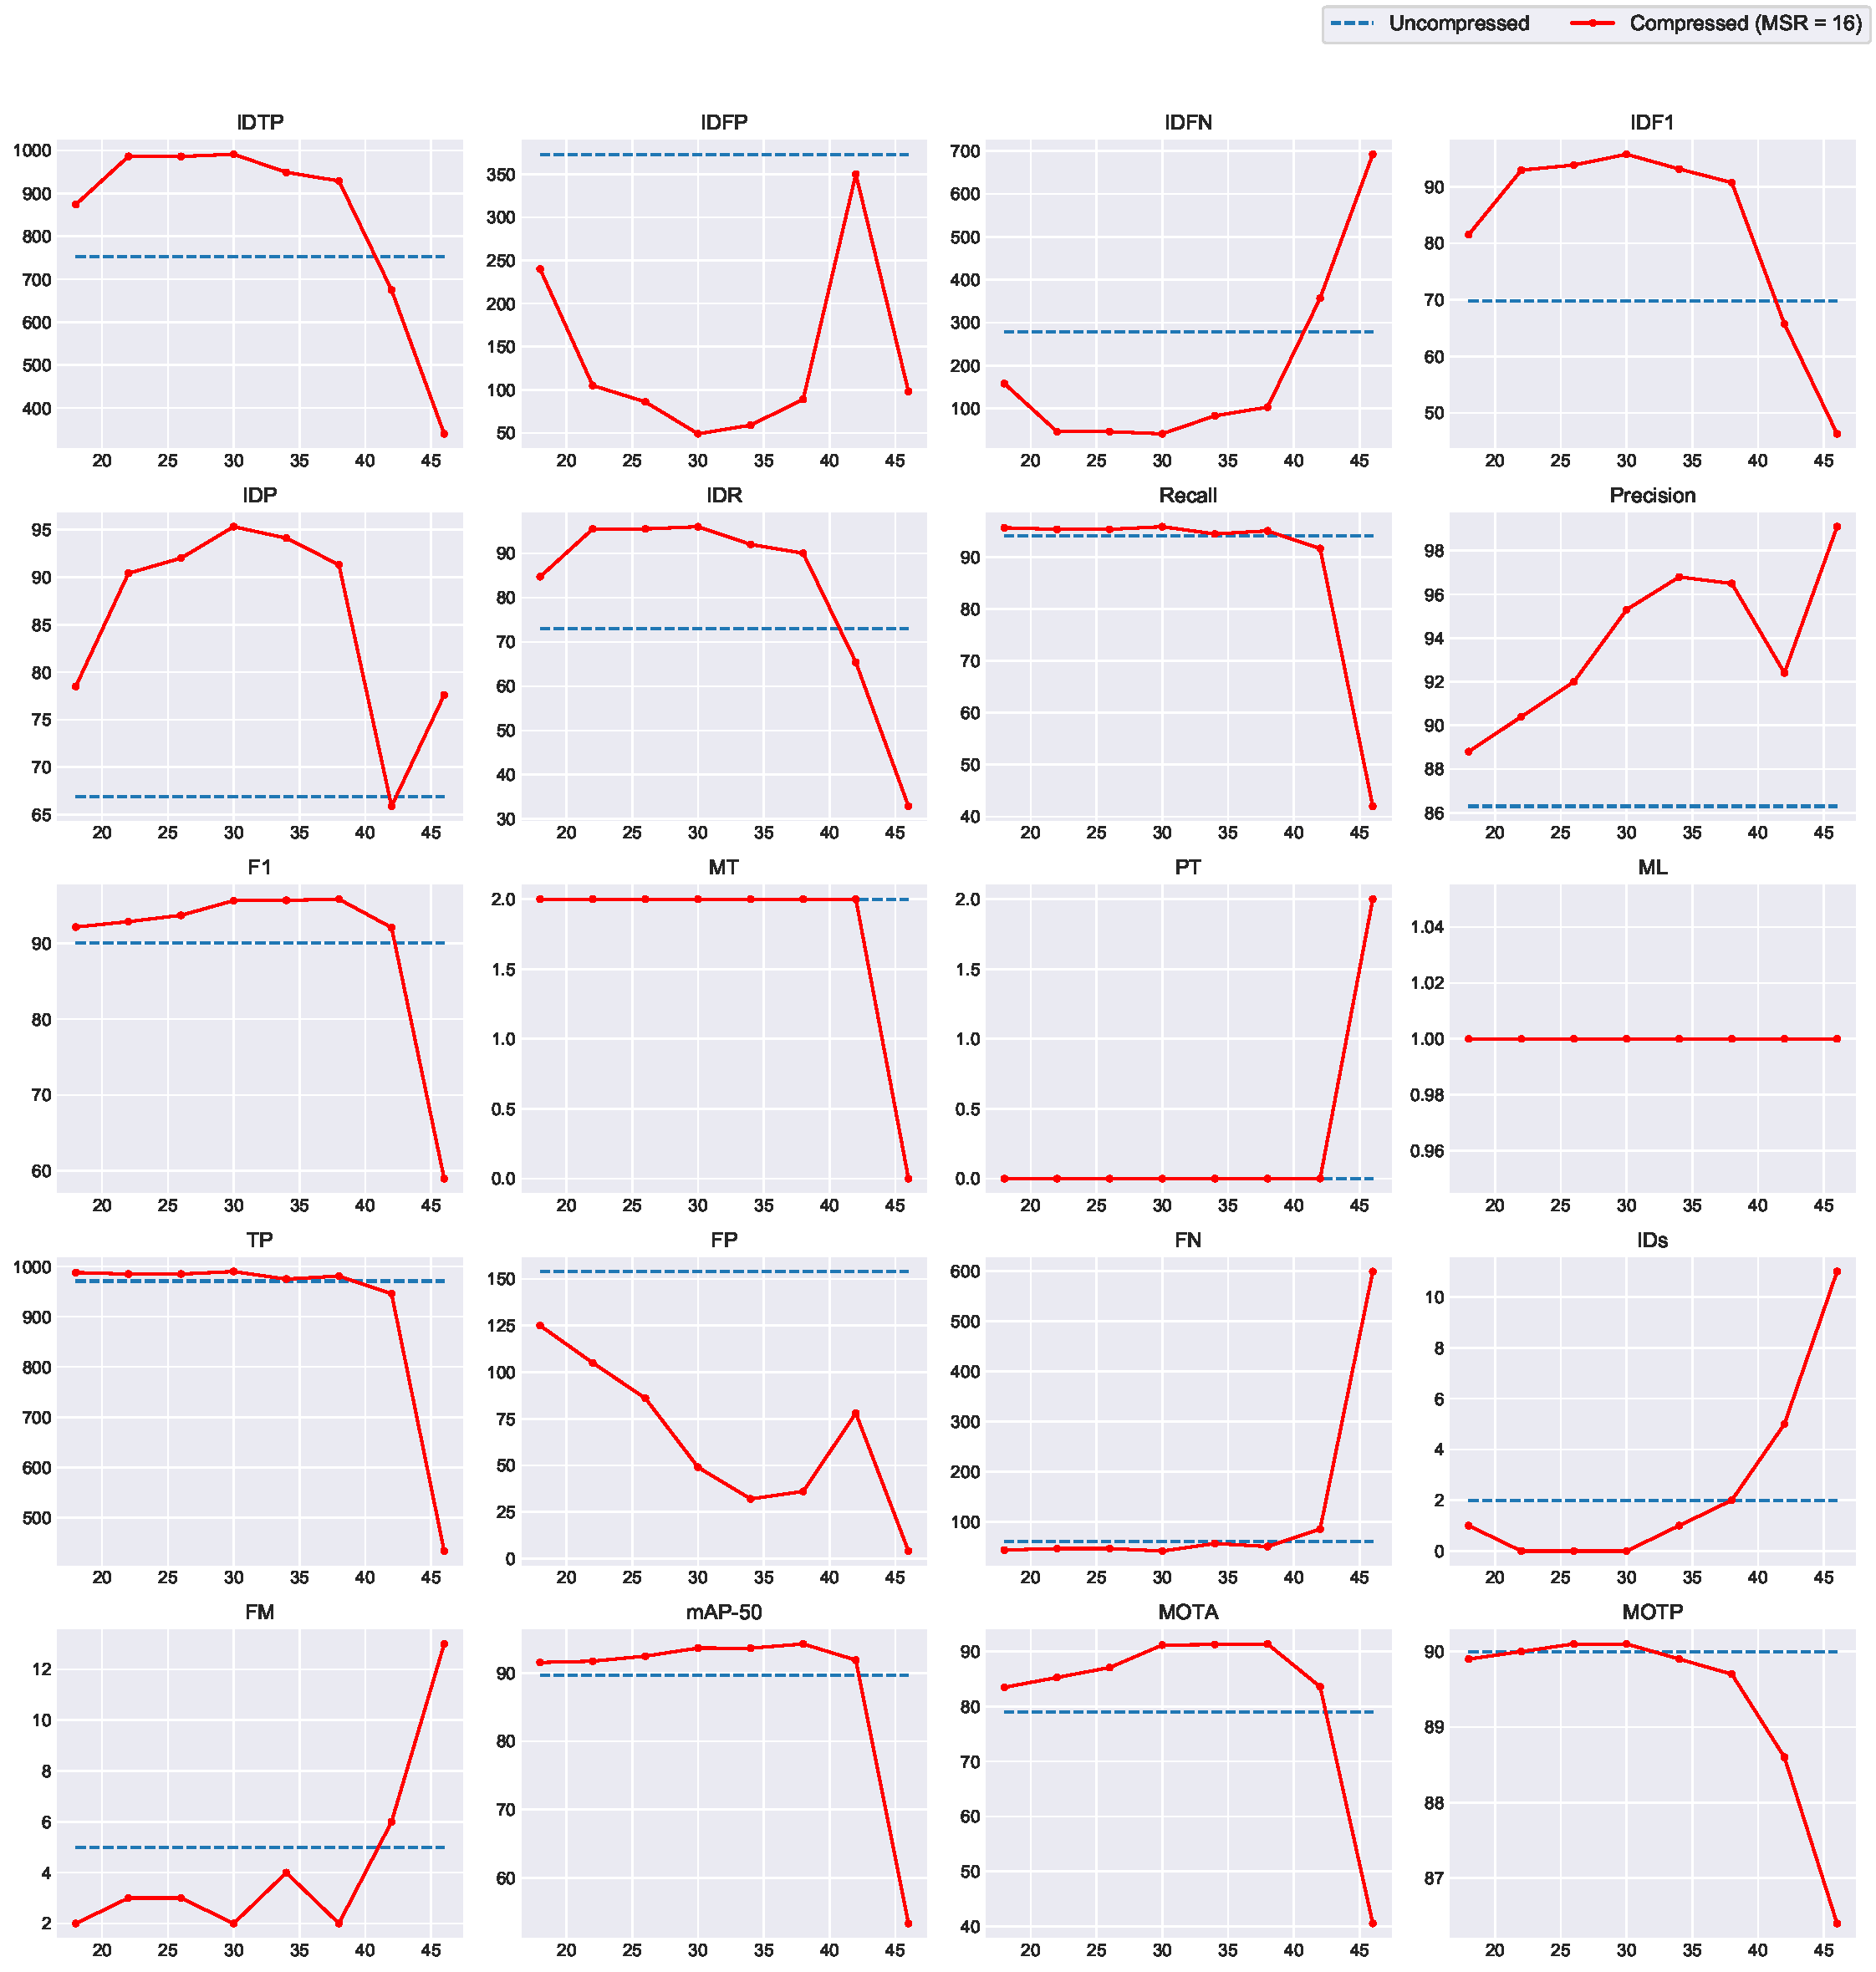
\includegraphics[width=1.0\linewidth]{img/BlowingBubbles_0_multiplots_qp.pdf}
  \caption[Visualization of the performance results on BlowingBubbles at different QP for the "person" object class]
  {
    Visualization of the performance results on BlowingBubbles at different QP for the "person" object class.
  }
  \label{fig:BlowingBubbles_0_multiplots_qp}
\end{figure}
\begin{table}[!htbp]
    \centering
    \caption[Performance results in Class D BlowingBubbles]
    {Performance results in Class D BlowingBubbles.}    \resizebox{1.0\linewidth}{!}{
    \begin{tabular}{llrrrrrrrrrrrrrrrrrrrr}
    \toprule
              QP &          MSR &   IDTP &   IDFP &   IDFN &  IDF1 &   IDP &   IDR &  Recall &  Precision &    F1 &  GT &  MT &  PT &  ML &  TP &  FP &  FN &  IDs &  FM &  MOTA &  MOTP \\
    \midrule
    Uncompressed & Uncompressed & 753.00 & 373.00 & 279.00 & 69.80 & 66.90 & 73.00 &   94.10 &      86.30 & 90.03 &   3 &   2 &   0 &   1 & 971 & 154 &  61 &    2 &   5 & 79.00 & 90.00 \\
              18 &           16 & 874.00 & 240.00 & 158.00 & 81.50 & 78.50 & 84.70 &   95.70 &      88.80 & 92.12 &   3 &   2 &   0 &   1 & 988 & 125 &  44 &    1 &   2 & 83.50 & 89.90 \\
              22 &           16 & 986.00 & 105.00 &  46.00 & 92.90 & 90.40 & 95.50 &   95.40 &      90.40 & 92.83 &   3 &   2 &   0 &   1 & 985 & 105 &  47 &    0 &   3 & 85.30 & 90.00 \\
              26 &           16 & 986.00 &  86.00 &  46.00 & 93.80 & 92.00 & 95.50 &   95.40 &      92.00 & 93.67 &   3 &   2 &   0 &   1 & 985 &  86 &  47 &    0 &   3 & 87.10 & 90.10 \\
              30 &           16 & 991.00 &  49.00 &  41.00 & 95.70 & 95.30 & 96.00 &   95.90 &      95.30 & 95.60 &   3 &   2 &   0 &   1 & 990 &  49 &  42 &    0 &   2 & 91.20 & 90.10 \\
              34 &           16 & 949.00 &  59.00 &  83.00 & 93.10 & 94.10 & 92.00 &   94.50 &      96.80 & 95.64 &   3 &   2 &   0 &   1 & 975 &  32 &  57 &    1 &   4 & 91.30 & 89.90 \\
              38 &           16 & 929.00 &  89.00 & 103.00 & 90.70 & 91.30 & 90.00 &   95.10 &      96.50 & 95.79 &   3 &   2 &   0 &   1 & 981 &  36 &  51 &    2 &   2 & 91.40 & 89.70 \\
              42 &           16 & 675.00 & 350.00 & 357.00 & 65.70 & 65.90 & 65.40 &   91.70 &      92.40 & 92.05 &   3 &   2 &   0 &   1 & 946 &  78 &  86 &    5 &   6 & 83.60 & 88.60 \\
              46 &           16 & 340.00 &  98.00 & 692.00 & 46.30 & 77.60 & 32.90 &   42.00 &      99.10 & 59.00 &   3 &   0 &   2 &   1 & 433 &   4 & 599 &   11 &  13 & 40.50 & 86.40 \\
    \bottomrule
    \end{tabular}
    }
    \label{tab:BlowingBubbles_0}
\end{table}
The MOTA visualization plot shows that the performance increases until QP = 38 but decreases thereafter. To verify this phenomenon, we inspected the video carefully by frame. From Figure \ref{fig:BlowingBubbles_0_frame465} that shows the sequence at frame 465, we observed a humanlike object that was detected as Person at the uncompressed case and QP = 18, 22, 26 but not thereafter.
\begin{figure}[!htbp]
  \centering
  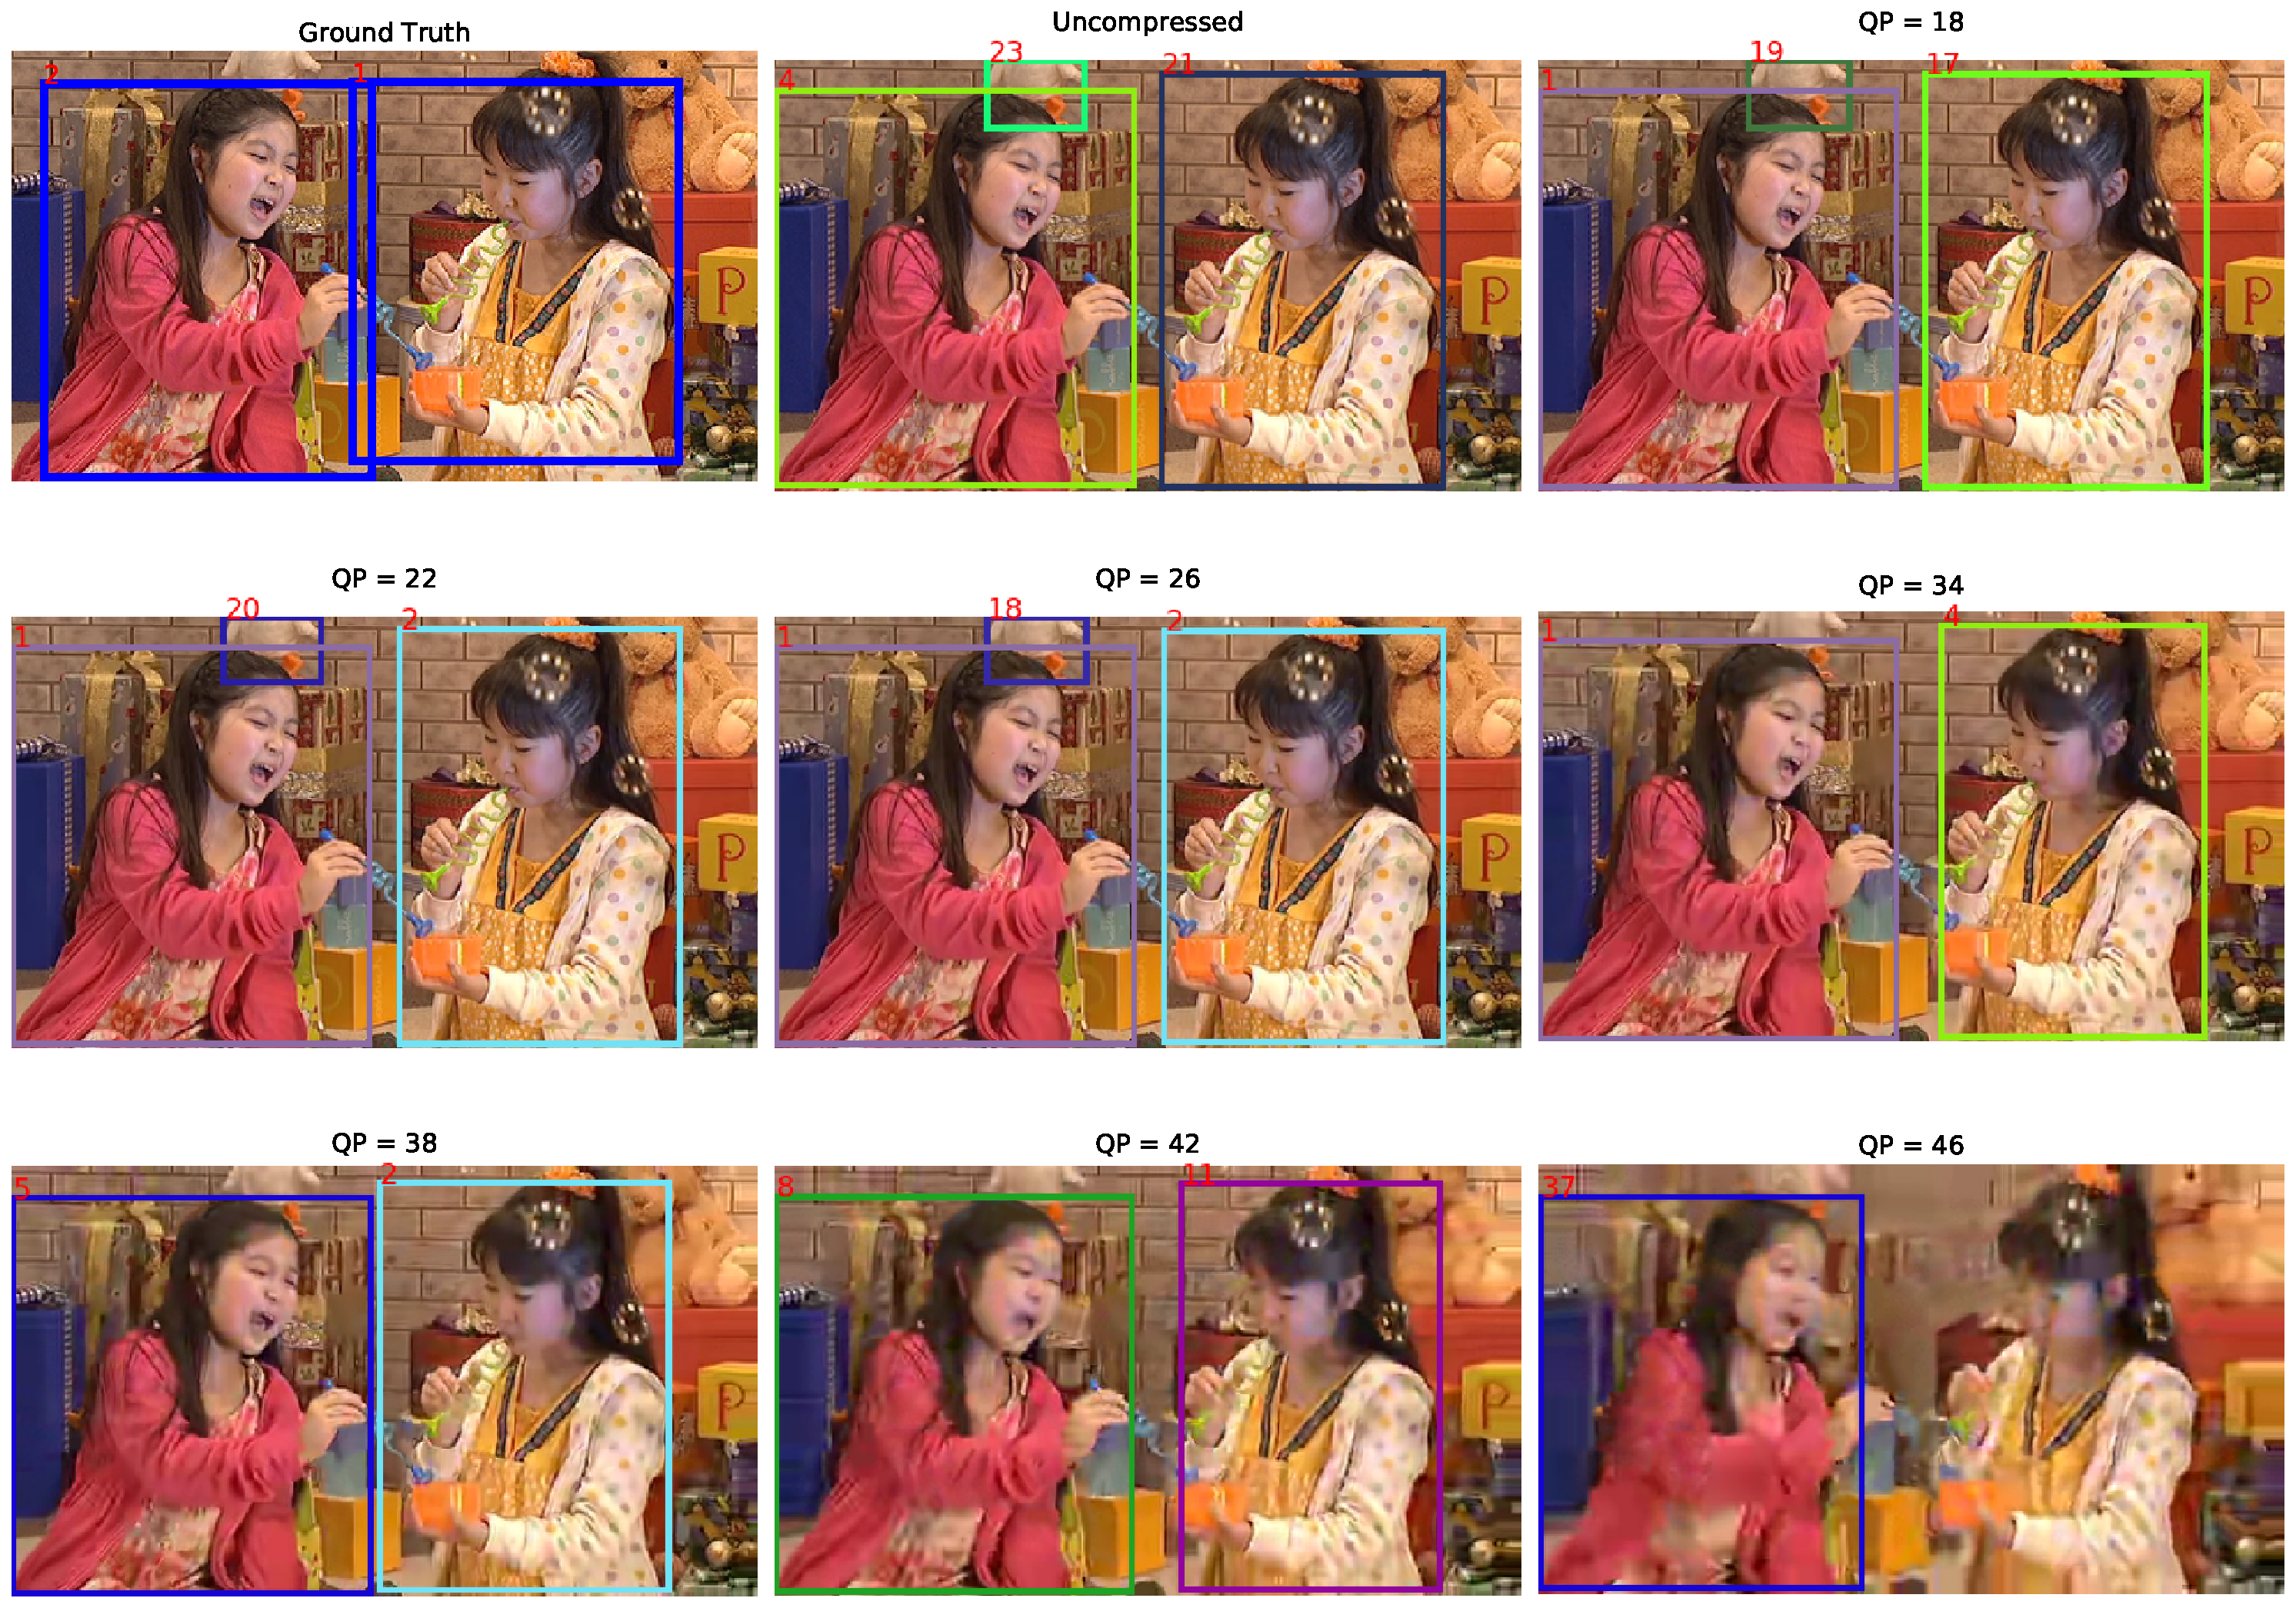
\includegraphics[width=1.0\linewidth]{img/BlowingBubbles_0_frame465.pdf}
  \caption[Comparison of Class D BlowingBubbles image frames at 465 at different QP]
  {
  Comparison of Class D BlowingBubbles image frames at 465 at different QP.
  }
  \label{fig:BlowingBubbles_0_frame465}
\end{figure}
This reveals that the detector incorrectly detect and recognize this object as Person at the lower QP, but as the image quality drops at the higher QP, the detector starts to not detect this particular object. Note that this humanlike object is not a part of the ground truth. This phenomenon was also observed in other frames. This observation proves that as QP increases, FP decreases, leading to the increase of MOTA until QP = 38. After QP = 38, the image quality further drops and as can be confirmed from Figure \ref{fig:BlowingBubbles_0_frame465}, 1 Person object is not detected at QP = 46, thereby FN increases. We observed that not only MOTA, the detection performance and ID measure also result in the same way such that the performance scores increase up to the middle of QP range and decrease thereafter. For IDs, though there is no occlusion, we observed IDs to be increasing due to the drop of the image quality that makes the detection discontinuous. Note that we observed a decrease of IDs at the middle of QP range and it is because the detector starts to not detecting the false object as Person and re-ID attempt decreases.


\subsection{Class B Cactus}


\section{Summary}
\label{sec:results/summary}

We presented the average tracking results of 12 video sequences for "all" object classes. Regression analysis was conducted to quantify the impact of QP and MSR on MOTA and formulate the relationship between MOTA and QP. One-sided t-test was conducted to identify the specific QP at which the performance on compressed sequences is lower than on uncompressed sequences with 95\% confidence. The results indicate that most metrics except Precision and MOTP are consistent with our expectation. To achieve a better understanding of the average results, we inspected four individual sequences. From each video, we saw that as the image quality drops, the detector starts to not detect the target, showing the increase of FN. We also found that there are cases that make certain performance scores increase as the image quality decreases. This is because the tracking performance depends on the detector's performance. Our detector YOLOv3 sometimes incorrectly detects wrong targets, but as the image quality drops, the frequency of wrong detections decreases. We also learned that for videos with frequent occlusions, IDs decreases due to fewer detections and therefore less detected occlusions as the image quality drops. However, for videos with fewer occlusions, IDs increases due to "gap" of trajectories, and different identities would be assigned to the trajectories. Note that because SORT does not have a re-ID feature for long-term occlusions or undetection, we observed such IDs result. Finally, the impact of detection performance on tracking performance was examined. From the scatter plots of MOTA and mAP-50, we observed a linear relationship in some videos. However, some videos show a non-linear relationship such that as mAP-50 increases, MOTA increases but the rate of increase of MOTA decreases. The more thorough analysis will need to be conducted to understand this outcome.

\chapter{Conclusion}
\label{chap:conclusion}

In this work, we studied the impact of video compression on multiple object tracking performance. We started with annotating the ground truth that is suitable for object tracking, conducted the experiment by running the HEVC codec at different QP and MSR to the uncompressed video sequences, and ran the multiple object tracker to the decoded sequences. Analyzing the results from the compressed and uncompressed video sequences, the visualization of average results across 12 video sequences shows that as QP increases, detection and tracking performance decrease, which is consistent with the expectation, except for the Precision and MOTP scores. Applying the regression analysis to all the video sequences, we learned that MSR does not impact the MOTA score but QP does with 95\% confidence based on the available data. We also proposed the formulation of MOTA and QP. One-sided t-test was also conducted to determine the specific QP at which detection and tracking performance on compressed sequences is lower than on uncompressed sequences. 

By analyzing further on four individual sequences as case studies, we illustrated that FN increases as QP increases due to less detection as the image quality drops. Since FN is significantly larger than the change in FP and IDs, we observed a decrease of MOTA. However, We found that MOTA sometimes increases midway through the QP range in some sequences. This is because the certain type of objects causes YOLOv3 to detect wrong objects, leading to a higher FP than the case on uncompressed video sequences. As the image quality drops, the frequency of incorrect detection decreases; hence, FP decreases and MOTA increases. However, as the image quality further drops, MOTA decreases due to the significant increase of FN. The reason the Precision score increased in the average results is also due to the decrease of FP. As we are analyzing the problem in the multiple objects, occlusion is inevitable in some video sequences. We found that IDs decreases in the video sequences with frequent occlusions due to the less detected occlusions as QP increases. For sequences with fewer occlusions, IDs increases as QP increases due to "gap" of trajectories caused by the drop of image quality. For MOTP, the increase of score midway through the QP range was observed. From the analysis of four individual sequences, we observed such increases in some sequences, which indicate that as the image quality drops, the object localization improves in some sequences, but further analysis is required to identify its cause. 

These case studies explained that the results are due to the design of YOLOv3 and SORT. Tracking performance is dependent on the design of the tracker. In our case, we are using a detection-based tracker; therefore, the tracking performance is dependent on the detection performance. Analyzing how detection impacts tracking performance, the linear and non-linear relationships of MOTA and mAP-50 were observed. The more thorough analysis will be necessary to identify the reason for the non-linear outcome, which is a decrease of MOTA growth rate as mAP-50 increases. The possible factors to consider could be size of bounding boxes and parameters in the Kalman filter framework in SORT.

We employed a simple and effective approach to detecting and tracking multiple objects using YOLOv3 and SORT; however, since there are better detectors and trackers, we could run the experiment with a better multiple object tracker. For example, for a detector, Ultralytics recently developed YOLOv5x6, achieving mAP of 54.4 and mAP-50 of 72.0 at a better resolution of $1280 \times 1280$ \cite{jocher_ultralyticsyolov5_2021}. This is a better performance than what we have in YOLOv3, i.e., mAP of 43.3 and mAP-50 of 63.0 at a resolution of $640 \times 640$. Since SORT does not have a feature to perform re-ID for the long-term occlusions and undetection, we could improve the tracker by implementing a re-ID feature. Finally, since QP and MSR are not the only configuration parameters in the video compression standard of HEVC, we could explore and examine further with different configurations.

\backmatter

\clearpage
\phantomsection
\addcontentsline{toc}{chapter}{References}
\printbibliography[title=References]

\appendix
\chapter{Multiple Classes Multiple Object Tracking Performance}
The additional information regarding the optimization of YOLOv3 and SORT is included in this section. Appendix \ref{sec:appendix/section_a} shows the initial attempt on 

\section{Justification of SORT Optimization}
\label{sec:appendix/section_a}

We optimized SORT by maximizing MOTA on the training video sequence of PartyScene as explained in Section \ref{sec:methods/section_b}. Since MOTA is not the only metric in MOT metrics, we will justify that other scores will achieve good performance at max age of 1, min hits of 5, and IOU threshold of 0.4. Table \ref{tab:optimizing_tracker_table} shows the results of all the performance metrics at different min hits. Note that we fixed max age of 1 as suggested by \cite{abewley_abewleysort_2021} and IOU threshold of 0.4 based on MOTA result.
\begin{table}[!hb]
  \centering
  \caption[Justification of SORT Optimization on “person” and “all” object classes.]
  {Justification of SORT Optimization on “person” and “all” object classes.}

  \begin{subtable}[t]{\linewidth}
    \centering
    \resizebox{1.0\linewidth}{!}{
    \begin{tabular}{rrrrrrrrrrrrrrrrrrr}
    \toprule
     max\_age &  min\_hits &  iou\_thres &  IDF1 &   IDP &   IDR &  Rcll &   Prcn &    F1 &  GT &  MT &  PT &  ML &  FP &  FN &  IDs &  FM &  MOTA &  MOTP \\
    \midrule
           1 &         1 &       0.40 & 80.70 & 81.40 & 80.10 & 95.50 &  97.20 & 96.34 &   3 &   3 &   0 &   0 &  21 &  34 &    6 &   9 & 92.00 & 86.60 \\
           1 &         2 &       0.40 & 81.40 & 83.20 & 79.80 & 94.60 &  98.60 & 96.56 &   3 &   3 &   0 &   0 &  10 &  41 &    6 &   8 & 92.50 & 86.70 \\
           1 &         3 &       0.40 & 81.80 & 84.30 & 79.50 & 93.60 &  99.20 & 96.32 &   3 &   2 &   1 &   0 &   6 &  49 &    6 &   6 & 92.00 & 86.80 \\
           1 &         4 &       0.40 & 82.10 & 85.10 & 79.30 & 92.80 &  99.60 & 96.08 &   3 &   2 &   1 &   0 &   3 &  55 &    4 &   4 & 91.90 & 86.80 \\
           1 &         5 &       0.40 & 82.20 & 85.50 & 79.10 & 92.30 &  99.70 & 95.86 &   3 &   2 &   1 &   0 &   2 &  59 &    4 &   4 & 91.50 & 86.80 \\
           1 &         6 &       0.40 & 82.40 & 86.00 & 79.00 & 91.70 &  99.90 & 95.62 &   3 &   2 &   1 &   0 &   1 &  63 &    4 &   4 & 91.10 & 86.90 \\
           1 &         7 &       0.40 & 82.50 & 86.50 & 78.90 & 91.20 & 100.00 & 95.40 &   3 &   2 &   1 &   0 &   0 &  67 &    3 &   3 & 90.80 & 86.90 \\
           1 &         8 &       0.40 & 82.50 & 86.70 & 78.70 & 90.80 & 100.00 & 95.18 &   3 &   2 &   1 &   0 &   0 &  70 &    3 &   3 & 90.40 & 86.90 \\
           1 &         9 &       0.40 & 82.60 & 86.90 & 78.60 & 90.40 & 100.00 & 94.96 &   3 &   1 &   2 &   0 &   0 &  73 &    3 &   3 & 90.00 & 86.90 \\
    \bottomrule
    \end{tabular}
    }
    \caption{Tuning parameters on "person" object class.}
  \end{subtable}
 
 
    \begin{subtable}[t]{\linewidth}
    \centering
    \resizebox{1.0\linewidth}{!}{
    \begin{tabular}{rrrrrrrrrrrrrrrrrrr}
    \toprule
     max\_age &  min\_hits &  iou\_thres &  IDF1 &   IDP &   IDR &  Rcll &  Prcn &    F1 &  GT &  MT &  PT &  ML &  FP &  FN &  IDs &  FM &  MOTA &  MOTP \\
    \midrule
           1 &         1 &       0.40 & 70.00 & 67.80 & 72.40 & 86.70 & 81.10 & 83.81 &   7 &   5 &   2 &   0 & 430 & 285 &   20 &  30 & 65.60 & 85.80 \\
           1 &         2 &       0.40 & 71.10 & 69.90 & 72.30 & 85.50 & 82.70 & 84.08 &   7 &   5 &   2 &   0 & 382 & 309 &   18 &  24 & 66.80 & 85.90 \\
           1 &         3 &       0.40 & 71.80 & 71.50 & 72.10 & 84.60 & 83.80 & 84.20 &   7 &   5 &   2 &   0 & 350 & 330 &   13 &  17 & 67.60 & 85.90 \\
           1 &         4 &       0.40 & 72.40 & 72.80 & 72.00 & 83.90 & 84.80 & 84.35 &   7 &   4 &   3 &   0 & 321 & 344 &   10 &  14 & 68.40 & 86.00 \\
           1 &         5 &       0.40 & 72.90 & 73.90 & 71.90 & 83.40 & 85.80 & 84.58 &   7 &   4 &   3 &   0 & 295 & 355 &   10 &  13 & 69.10 & 86.00 \\
           1 &         6 &       0.40 & 73.40 & 75.10 & 71.80 & 83.00 & 86.80 & 84.86 &   7 &   4 &   3 &   0 & 270 & 364 &   11 &  12 & 69.80 & 86.10 \\
           1 &         7 &       0.40 & 73.90 & 76.20 & 71.70 & 82.50 & 87.70 & 85.02 &   7 &   4 &   3 &   0 & 247 & 373 &   10 &  12 & 70.50 & 86.10 \\
           1 &         8 &       0.40 & 74.30 & 77.10 & 71.60 & 82.10 & 88.50 & 85.18 &   7 &   4 &   3 &   0 & 228 & 382 &   10 &  12 & 71.00 & 86.10 \\
           1 &         9 &       0.40 & 74.60 & 78.00 & 71.50 & 81.70 & 89.10 & 85.24 &   7 &   4 &   3 &   0 & 213 & 391 &   10 &  12 & 71.30 & 86.10 \\
    \bottomrule
    \end{tabular}
    }
    \caption{Tuning parameters on "all" object class.}
  \end{subtable}
 \label{tab:optimizing_tracker_table}  
\end{table}
\section{section b}
\label{sec:appendix/section_b}

\chapter{All Results of Individual Sequences}

\newpage

\section{Class B BasketballDrive}
\label{sec:appendix/BasketballDrive_all}


% visualization figure
\begin{figure}[!htbp]
\centering
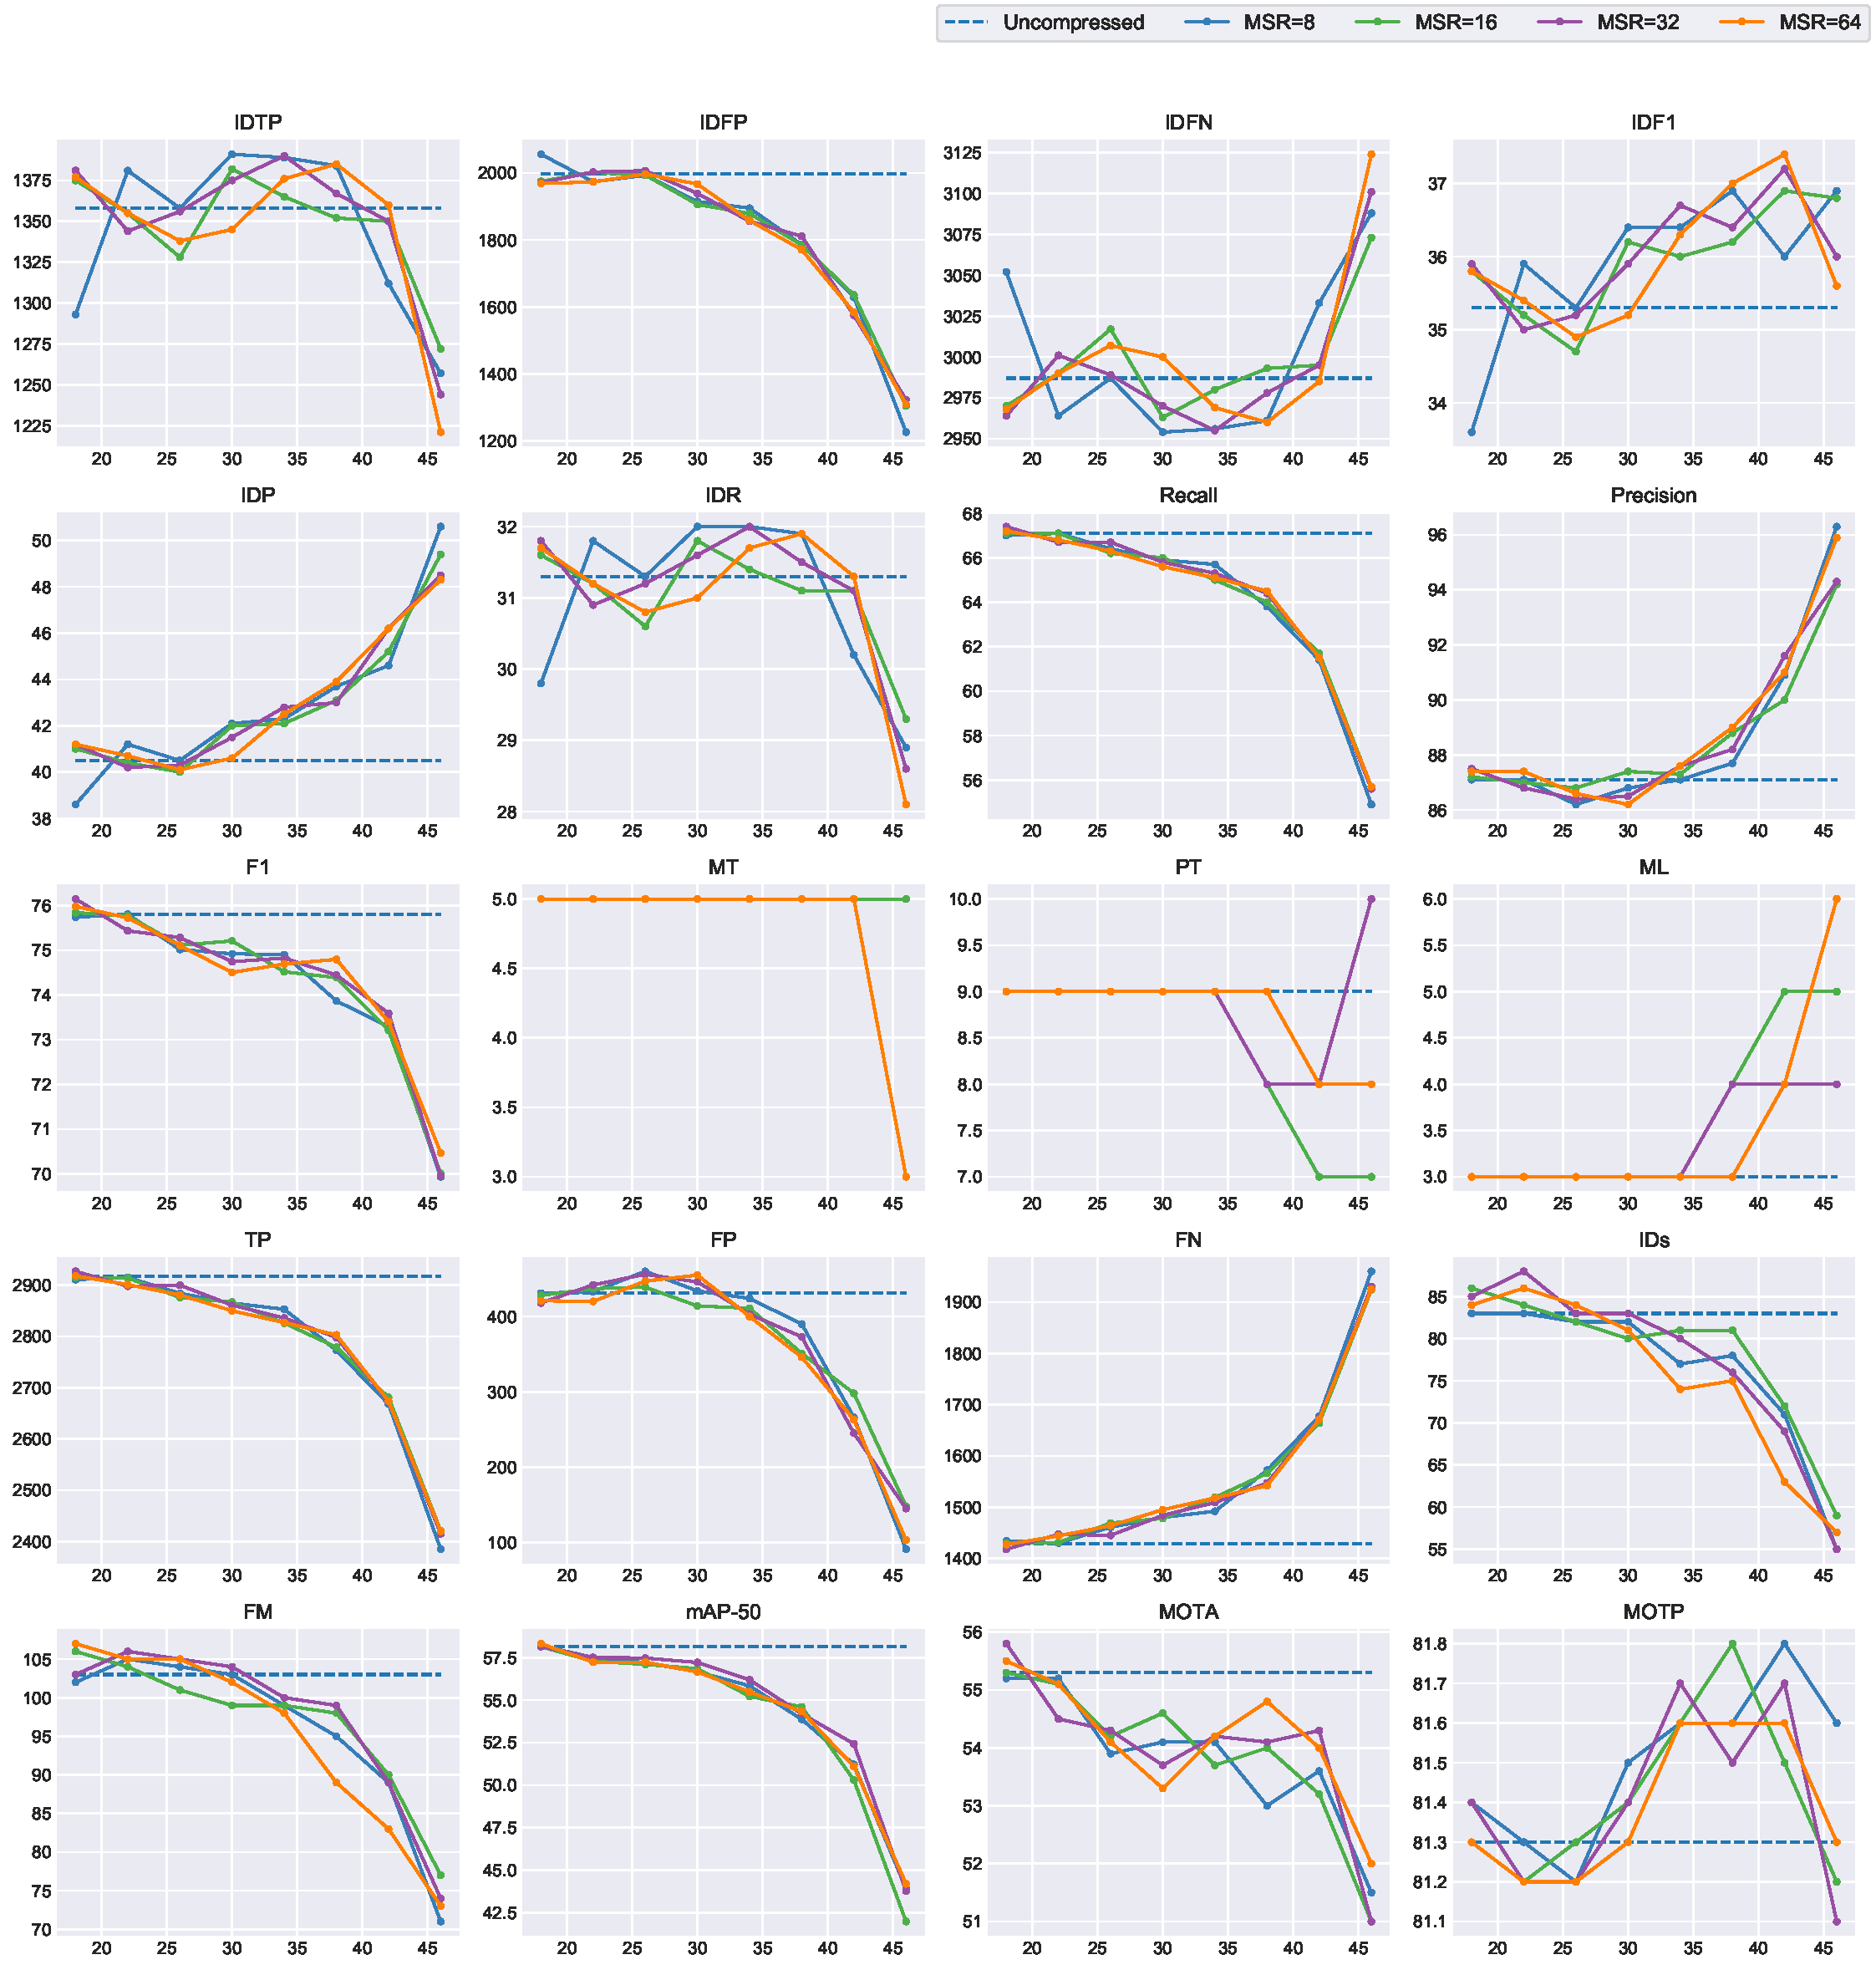
\includegraphics[width=1.0\linewidth]{img/appendix/BasketballDrive_all_multiplots_qp.pdf}
\caption[Result of all object classes in Class B BasketballDrive with Horizontal Axis of QP]{}
\label{fig:BasketballDrive_all_qp}
\end{figure}

\begin{figure}[!htbp]
\centering
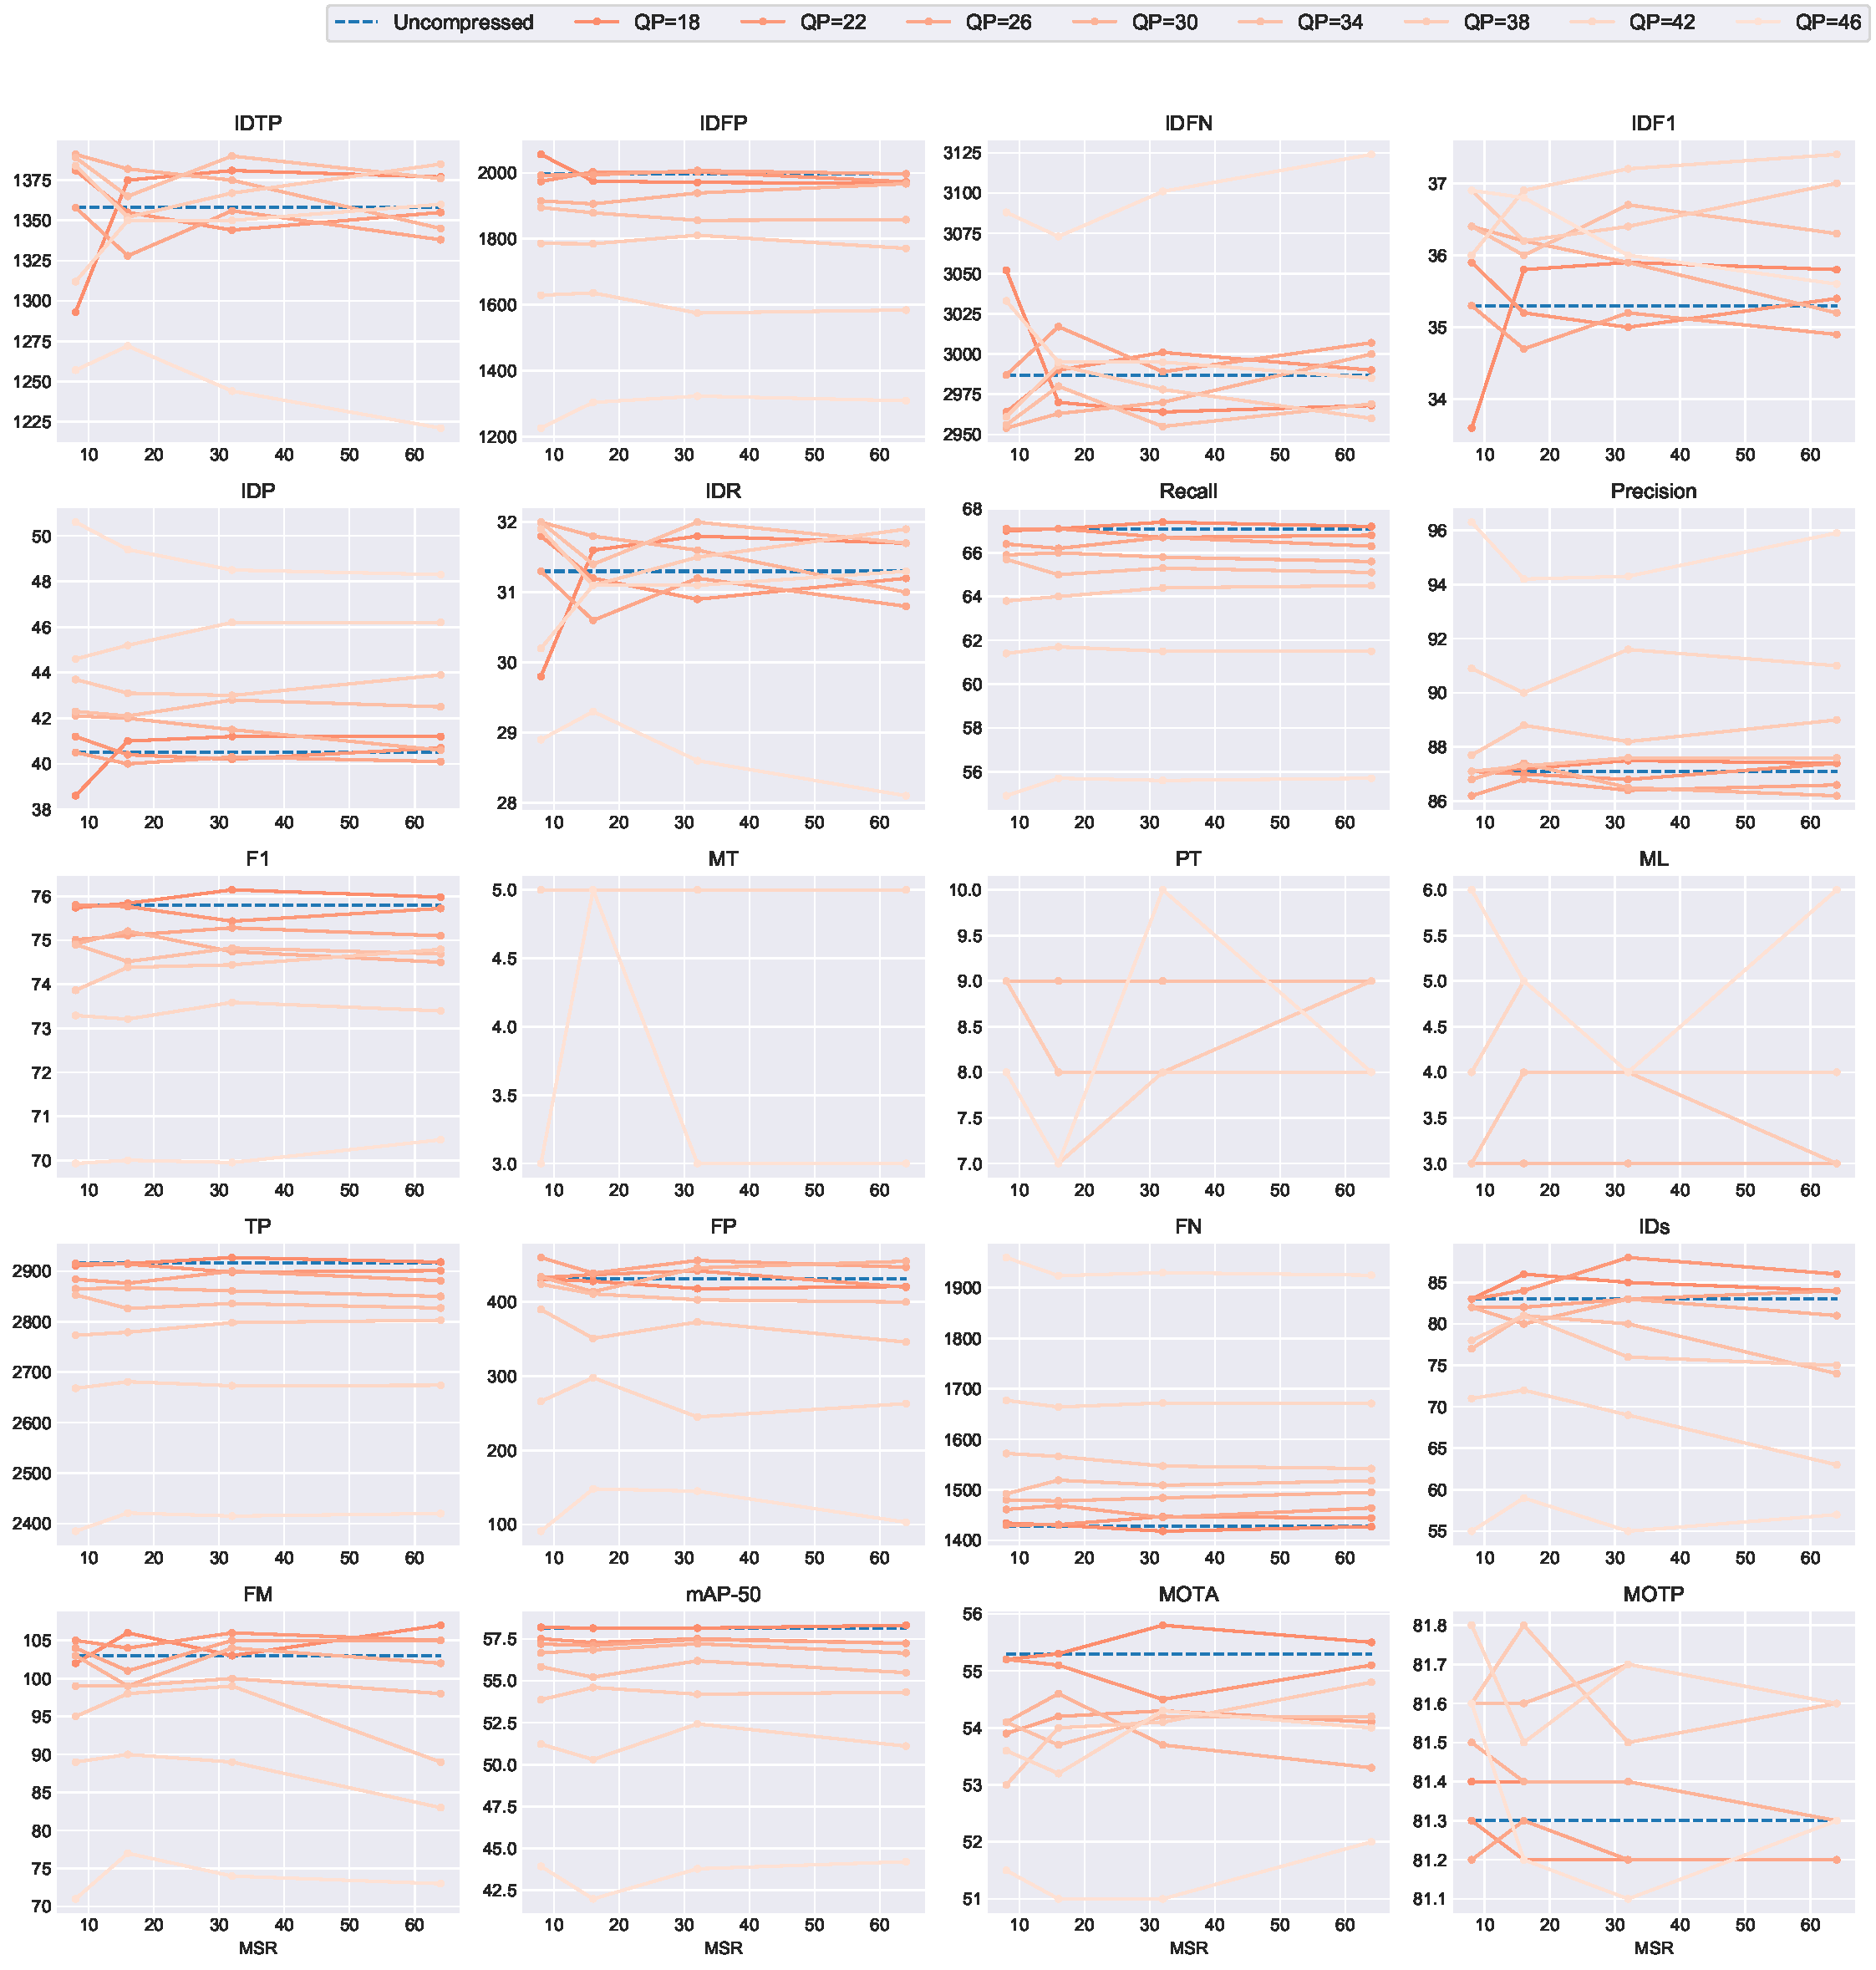
\includegraphics[width=1.0\linewidth]{img/appendix/BasketballDrive_all_multiplots_msr.pdf}
\caption[Result of all object classes in Class B BasketballDrive with Horizontal Axis of MSR]{}
\label{fig:BasketballDrive_all_msr}
\end{figure}



% table
\begin{table}
\centering
\caption{Result of all object classes in Class B BasketballDrive}


% table for uncompressed
\begin{subtable}[t]{\linewidth}
\centering
\vspace{0pt}
\resizebox{1.0\linewidth}{!}{
\begin{tabular}{llrrrrrrrrrrrrrrrrrrrr}
\toprule
          QP &          MSR &    IDTP &    IDFP &    IDFN &  IDF1 &   IDP &   IDR &  Recall &  Precision &    F1 &  GT &  MT &  PT &  ML &   TP &  FP &   FN &  IDs &  FM &  MOTA &  MOTP \\
\midrule
Uncompressed & Uncompressed & 1358.00 & 1997.00 & 2987.00 & 35.30 & 40.50 & 31.30 &   67.10 &      87.10 & 75.80 &  17 &   5 &   9 &   3 & 2917 & 431 & 1428 &   83 & 103 & 55.30 & 81.30 \\
\bottomrule
\end{tabular}

}
\caption{Uncompressed Sequence}
\end{subtable}


% table for msr=8
\begin{subtable}[t]{\linewidth}
\centering
\resizebox{1.0\linewidth}{!}{
\begin{tabular}{rrrrrrrrrrrrrrrrrrrrrr}
\toprule
 QP &  MSR &    IDTP &    IDFP &    IDFN &  IDF1 &   IDP &   IDR &  Recall &  Precision &    F1 &  GT &  MT &  PT &  ML &   TP &  FP &   FN &  IDs &  FM &  MOTA &  MOTP \\
\midrule
 18 &    8 & 1293.00 & 2056.00 & 3052.00 & 33.60 & 38.60 & 29.80 &   67.00 &      87.10 & 75.74 &  17 &   5 &   9 &   3 & 2911 & 431 & 1434 &   83 & 102 & 55.20 & 81.40 \\
 22 &    8 & 1381.00 & 1974.00 & 2964.00 & 35.90 & 41.20 & 31.80 &   67.10 &      87.10 & 75.80 &  17 &   5 &   9 &   3 & 2915 & 433 & 1430 &   83 & 105 & 55.20 & 81.30 \\
 26 &    8 & 1358.00 & 1993.00 & 2987.00 & 35.30 & 40.50 & 31.30 &   66.40 &      86.20 & 75.02 &  17 &   5 &   9 &   3 & 2884 & 460 & 1461 &   82 & 104 & 53.90 & 81.20 \\
 30 &    8 & 1391.00 & 1915.00 & 2954.00 & 36.40 & 42.10 & 32.00 &   65.90 &      86.80 & 74.92 &  17 &   5 &   9 &   3 & 2865 & 434 & 1480 &   82 & 103 & 54.10 & 81.50 \\
 34 &    8 & 1389.00 & 1895.00 & 2956.00 & 36.40 & 42.30 & 32.00 &   65.70 &      87.10 & 74.90 &  17 &   5 &   9 &   3 & 2853 & 424 & 1492 &   77 &  99 & 54.10 & 81.60 \\
 38 &    8 & 1384.00 & 1786.00 & 2961.00 & 36.90 & 43.70 & 31.90 &   63.80 &      87.70 & 73.86 &  17 &   5 &   9 &   3 & 2773 & 390 & 1572 &   78 &  95 & 53.00 & 81.60 \\
 42 &    8 & 1312.00 & 1629.00 & 3033.00 & 36.00 & 44.60 & 30.20 &   61.40 &      90.90 & 73.29 &  17 &   5 &   8 &   4 & 2668 & 266 & 1677 &   71 &  89 & 53.60 & 81.80 \\
 46 &    8 & 1257.00 & 1226.00 & 3088.00 & 36.90 & 50.60 & 28.90 &   54.90 &      96.30 & 69.93 &  17 &   3 &   8 &   6 & 2385 &  91 & 1960 &   55 &  71 & 51.50 & 81.60 \\
\bottomrule
\end{tabular}

}
\caption{MSR = 8}
\end{subtable}



% table for msr=16
\begin{subtable}[t]{\linewidth}
\centering
\resizebox{1.0\linewidth}{!}{
\begin{tabular}{rrrrrrrrrrrrrrrrrrrrrr}
\toprule
 QP &  MSR &    IDTP &    IDFP &    IDFN &  IDF1 &   IDP &   IDR &  Recall &  Precision &    F1 &  GT &  MT &  PT &  ML &   TP &  FP &   FN &  IDs &  FM &  MOTA &  MOTP \\
\midrule
 18 &   16 & 1375.00 & 1975.00 & 2970.00 & 35.80 & 41.00 & 31.60 &   67.10 &      87.20 & 75.84 &  17 &   5 &   9 &   3 & 2915 & 428 & 1430 &   86 & 106 & 55.30 & 81.40 \\
 22 &   16 & 1355.00 & 2003.00 & 2990.00 & 35.20 & 40.40 & 31.20 &   67.10 &      87.00 & 75.77 &  17 &   5 &   9 &   3 & 2914 & 437 & 1431 &   84 & 104 & 55.10 & 81.20 \\
 26 &   16 & 1328.00 & 1994.00 & 3017.00 & 34.70 & 40.00 & 30.60 &   66.20 &      86.80 & 75.11 &  17 &   5 &   9 &   3 & 2876 & 439 & 1469 &   82 & 101 & 54.20 & 81.30 \\
 30 &   16 & 1382.00 & 1906.00 & 2963.00 & 36.20 & 42.00 & 31.80 &   66.00 &      87.40 & 75.21 &  17 &   5 &   9 &   3 & 2867 & 414 & 1478 &   80 &  99 & 54.60 & 81.40 \\
 34 &   16 & 1365.00 & 1879.00 & 2980.00 & 36.00 & 42.10 & 31.40 &   65.00 &      87.30 & 74.52 &  17 &   5 &   9 &   3 & 2826 & 411 & 1519 &   81 &  99 & 53.70 & 81.60 \\
 38 &   16 & 1352.00 & 1785.00 & 2993.00 & 36.20 & 43.10 & 31.10 &   64.00 &      88.80 & 74.39 &  17 &   5 &   8 &   4 & 2779 & 351 & 1566 &   81 &  98 & 54.00 & 81.80 \\
 42 &   16 & 1350.00 & 1636.00 & 2995.00 & 36.90 & 45.20 & 31.10 &   61.70 &      90.00 & 73.21 &  17 &   5 &   7 &   5 & 2681 & 298 & 1664 &   72 &  90 & 53.20 & 81.50 \\
 46 &   16 & 1272.00 & 1304.00 & 3073.00 & 36.80 & 49.40 & 29.30 &   55.70 &      94.20 & 70.01 &  17 &   5 &   7 &   5 & 2421 & 148 & 1924 &   59 &  77 & 51.00 & 81.20 \\
\bottomrule
\end{tabular}

}
\caption{MSR = 16}
\end{subtable}


% table for msr=32
\begin{subtable}[t]{\linewidth}
\centering
\resizebox{1.0\linewidth}{!}{
\begin{tabular}{rrrrrrrrrrrrrrrrrrrrrr}
\toprule
 QP &  MSR &    IDTP &    IDFP &    IDFN &  IDF1 &   IDP &   IDR &  Recall &  Precision &    F1 &  GT &  MT &  PT &  ML &   TP &  FP &   FN &  IDs &  FM &  MOTA &  MOTP \\
\midrule
 18 &   32 & 1381.00 & 1971.00 & 2964.00 & 35.90 & 41.20 & 31.80 &   67.40 &      87.50 & 76.15 &  17 &   5 &   9 &   3 & 2927 & 418 & 1418 &   85 & 103 & 55.80 & 81.40 \\
 22 &   32 & 1344.00 & 2003.00 & 3001.00 & 35.00 & 40.20 & 30.90 &   66.70 &      86.80 & 75.43 &  17 &   5 &   9 &   3 & 2898 & 442 & 1447 &   88 & 106 & 54.50 & 81.20 \\
 26 &   32 & 1356.00 & 2007.00 & 2989.00 & 35.20 & 40.30 & 31.20 &   66.70 &      86.40 & 75.28 &  17 &   5 &   9 &   3 & 2900 & 456 & 1445 &   83 & 105 & 54.30 & 81.20 \\
 30 &   32 & 1375.00 & 1939.00 & 2970.00 & 35.90 & 41.50 & 31.60 &   65.80 &      86.50 & 74.74 &  17 &   5 &   9 &   3 & 2861 & 446 & 1484 &   83 & 104 & 53.70 & 81.40 \\
 34 &   32 & 1390.00 & 1856.00 & 2955.00 & 36.70 & 42.80 & 32.00 &   65.30 &      87.60 & 74.82 &  17 &   5 &   9 &   3 & 2836 & 403 & 1509 &   80 & 100 & 54.20 & 81.70 \\
 38 &   32 & 1367.00 & 1811.00 & 2978.00 & 36.40 & 43.00 & 31.50 &   64.40 &      88.20 & 74.44 &  17 &   5 &   8 &   4 & 2798 & 373 & 1547 &   76 &  99 & 54.10 & 81.50 \\
 42 &   32 & 1350.00 & 1575.00 & 2995.00 & 37.20 & 46.20 & 31.10 &   61.50 &      91.60 & 73.59 &  17 &   5 &   8 &   4 & 2673 & 245 & 1672 &   69 &  89 & 54.30 & 81.70 \\
 46 &   32 & 1244.00 & 1323.00 & 3101.00 & 36.00 & 48.50 & 28.60 &   55.60 &      94.30 & 69.95 &  17 &   3 &  10 &   4 & 2415 & 145 & 1930 &   55 &  74 & 51.00 & 81.10 \\
\bottomrule
\end{tabular}

}
\caption{MSR = 32}
\end{subtable}


% table for msr=64
\begin{subtable}[t]{\linewidth}
\centering
\resizebox{1.0\linewidth}{!}{
\begin{tabular}{rrrrrrrrrrrrrrrrrrrrrr}
\toprule
 QP &  MSR &    IDTP &    IDFP &    IDFN &  IDF1 &   IDP &   IDR &  Recall &  Precision &    F1 &  GT &  MT &  PT &  ML &   TP &  FP &   FN &  IDs &  FM &  MOTA &  MOTP \\
\midrule
 18 &   64 & 1377.00 & 1969.00 & 2968.00 & 35.80 & 41.20 & 31.70 &   67.20 &      87.40 & 75.98 &  17 &   5 &   9 &   3 & 2918 & 421 & 1427 &   84 & 107 & 55.50 & 81.30 \\
 22 &   64 & 1355.00 & 1973.00 & 2990.00 & 35.40 & 40.70 & 31.20 &   66.80 &      87.40 & 75.72 &  17 &   5 &   9 &   3 & 2901 & 420 & 1444 &   86 & 105 & 55.10 & 81.20 \\
 26 &   64 & 1338.00 & 1997.00 & 3007.00 & 34.90 & 40.10 & 30.80 &   66.30 &      86.60 & 75.10 &  17 &   5 &   9 &   3 & 2881 & 447 & 1464 &   84 & 105 & 54.10 & 81.20 \\
 30 &   64 & 1345.00 & 1967.00 & 3000.00 & 35.20 & 40.60 & 31.00 &   65.60 &      86.20 & 74.50 &  17 &   5 &   9 &   3 & 2850 & 455 & 1495 &   81 & 102 & 53.30 & 81.30 \\
 34 &   64 & 1376.00 & 1858.00 & 2969.00 & 36.30 & 42.50 & 31.70 &   65.10 &      87.60 & 74.69 &  17 &   5 &   9 &   3 & 2827 & 400 & 1518 &   74 &  98 & 54.20 & 81.60 \\
 38 &   64 & 1385.00 & 1771.00 & 2960.00 & 37.00 & 43.90 & 31.90 &   64.50 &      89.00 & 74.79 &  17 &   5 &   9 &   3 & 2803 & 346 & 1542 &   75 &  89 & 54.80 & 81.60 \\
 42 &   64 & 1360.00 & 1584.00 & 2985.00 & 37.40 & 46.20 & 31.30 &   61.50 &      91.00 & 73.40 &  17 &   5 &   8 &   4 & 2674 & 263 & 1671 &   63 &  83 & 54.00 & 81.60 \\
 46 &   64 & 1221.00 & 1309.00 & 3124.00 & 35.60 & 48.30 & 28.10 &   55.70 &      95.90 & 70.47 &  17 &   3 &   8 &   6 & 2420 & 103 & 1925 &   57 &  73 & 52.00 & 81.30 \\
\bottomrule
\end{tabular}

}
\caption{MSR = 64}
\end{subtable}


\label{tab:BasketballDrive_all}
\end{table}




\begin{table}[!htbp]
\centering
\caption{Multiple Linear Regression Analysis Result for Class B BasketballDrive}
\resizebox{1.0\linewidth}{!}{
\begin{tabular}{lrrrrrrrrrrrrrrrrrrr}
\toprule
{} &    IDTP &    IDFP &    IDFN &  IDF1 &   IDP &   IDR &  Recall &  Precision &    F1 &    MT &    PT &    ML &      TP &     FP &      FN &    IDs &     FM &  MOTA &  MOTP \\
\midrule
coefficient(Intercept) & 1401.88 & 2552.07 & 2943.12 & 33.55 & 33.06 & 32.28 &   75.44 &      81.12 & 79.72 &  5.57 & 10.20 &  1.24 & 3277.64 & 669.31 & 1067.36 & 101.97 & 123.60 & 57.73 & 81.16 \\
coefficient(QP)        &   -1.69 &  -23.13 &    1.69 &  0.08 &  0.31 & -0.04 &   -0.36 &       0.23 & -0.17 & -0.02 & -0.05 &  0.07 &  -15.43 &  -9.39 &   15.43 &  -0.76 &  -0.83 & -0.12 &  0.01 \\
coefficient(MSR)       &    0.55 &   -0.93 &   -0.55 &  0.02 &  0.02 &  0.01 &   -0.01 &      -0.00 & -0.01 &  0.01 & -0.01 &  0.00 &   -0.45 &   0.06 &    0.45 &   0.11 &   0.14 & -0.02 & -0.00 \\
coefficient(QP*MSR)    &   -0.02 &    0.03 &    0.02 & -0.00 & -0.00 & -0.00 &    0.00 &       0.00 &  0.00 & -0.00 &  0.00 & -0.00 &    0.01 &  -0.01 &   -0.01 &  -0.00 &  -0.00 &  0.00 & -0.00 \\
p-value(Intercept)     &    0.00 &    0.00 &    0.00 &  0.00 &  0.00 &  0.00 &    0.00 &       0.00 &  0.00 &  0.00 &  0.00 &  0.08 &    0.00 &   0.00 &    0.00 &   0.00 &   0.00 &  0.00 &  0.00 \\
p-value(QP)            &    0.23 &    0.00 &    0.23 &  0.00 &  0.00 &  0.23 &    0.00 &       0.00 &  0.00 &  0.23 &  0.01 &  0.00 &    0.00 &   0.00 &    0.00 &   0.00 &   0.00 &  0.00 &  0.12 \\
p-value(MSR)           &    0.66 &    0.80 &    0.66 &  0.38 &  0.58 &  0.66 &    0.88 &       0.95 &  0.79 &  0.61 &  0.59 &  0.97 &    0.87 &   0.98 &    0.87 &   0.47 &   0.39 &  0.49 &  0.90 \\
p-value(QP*MSR)        &    0.63 &    0.81 &    0.63 &  0.37 &  0.57 &  0.64 &    0.86 &       0.88 &  0.72 &  0.52 &  0.46 &  0.92 &    0.85 &   0.91 &    0.85 &   0.34 &   0.32 &  0.34 &  0.87 \\
\bottomrule
\end{tabular}

}
\label{tab:BasketballDrive_all_reg}
\end{table}



\newpage

\section{Class B Cactus}
\label{sec:appendix/Cactus_all}


% visualization figure
\begin{figure}[!htbp]
\centering
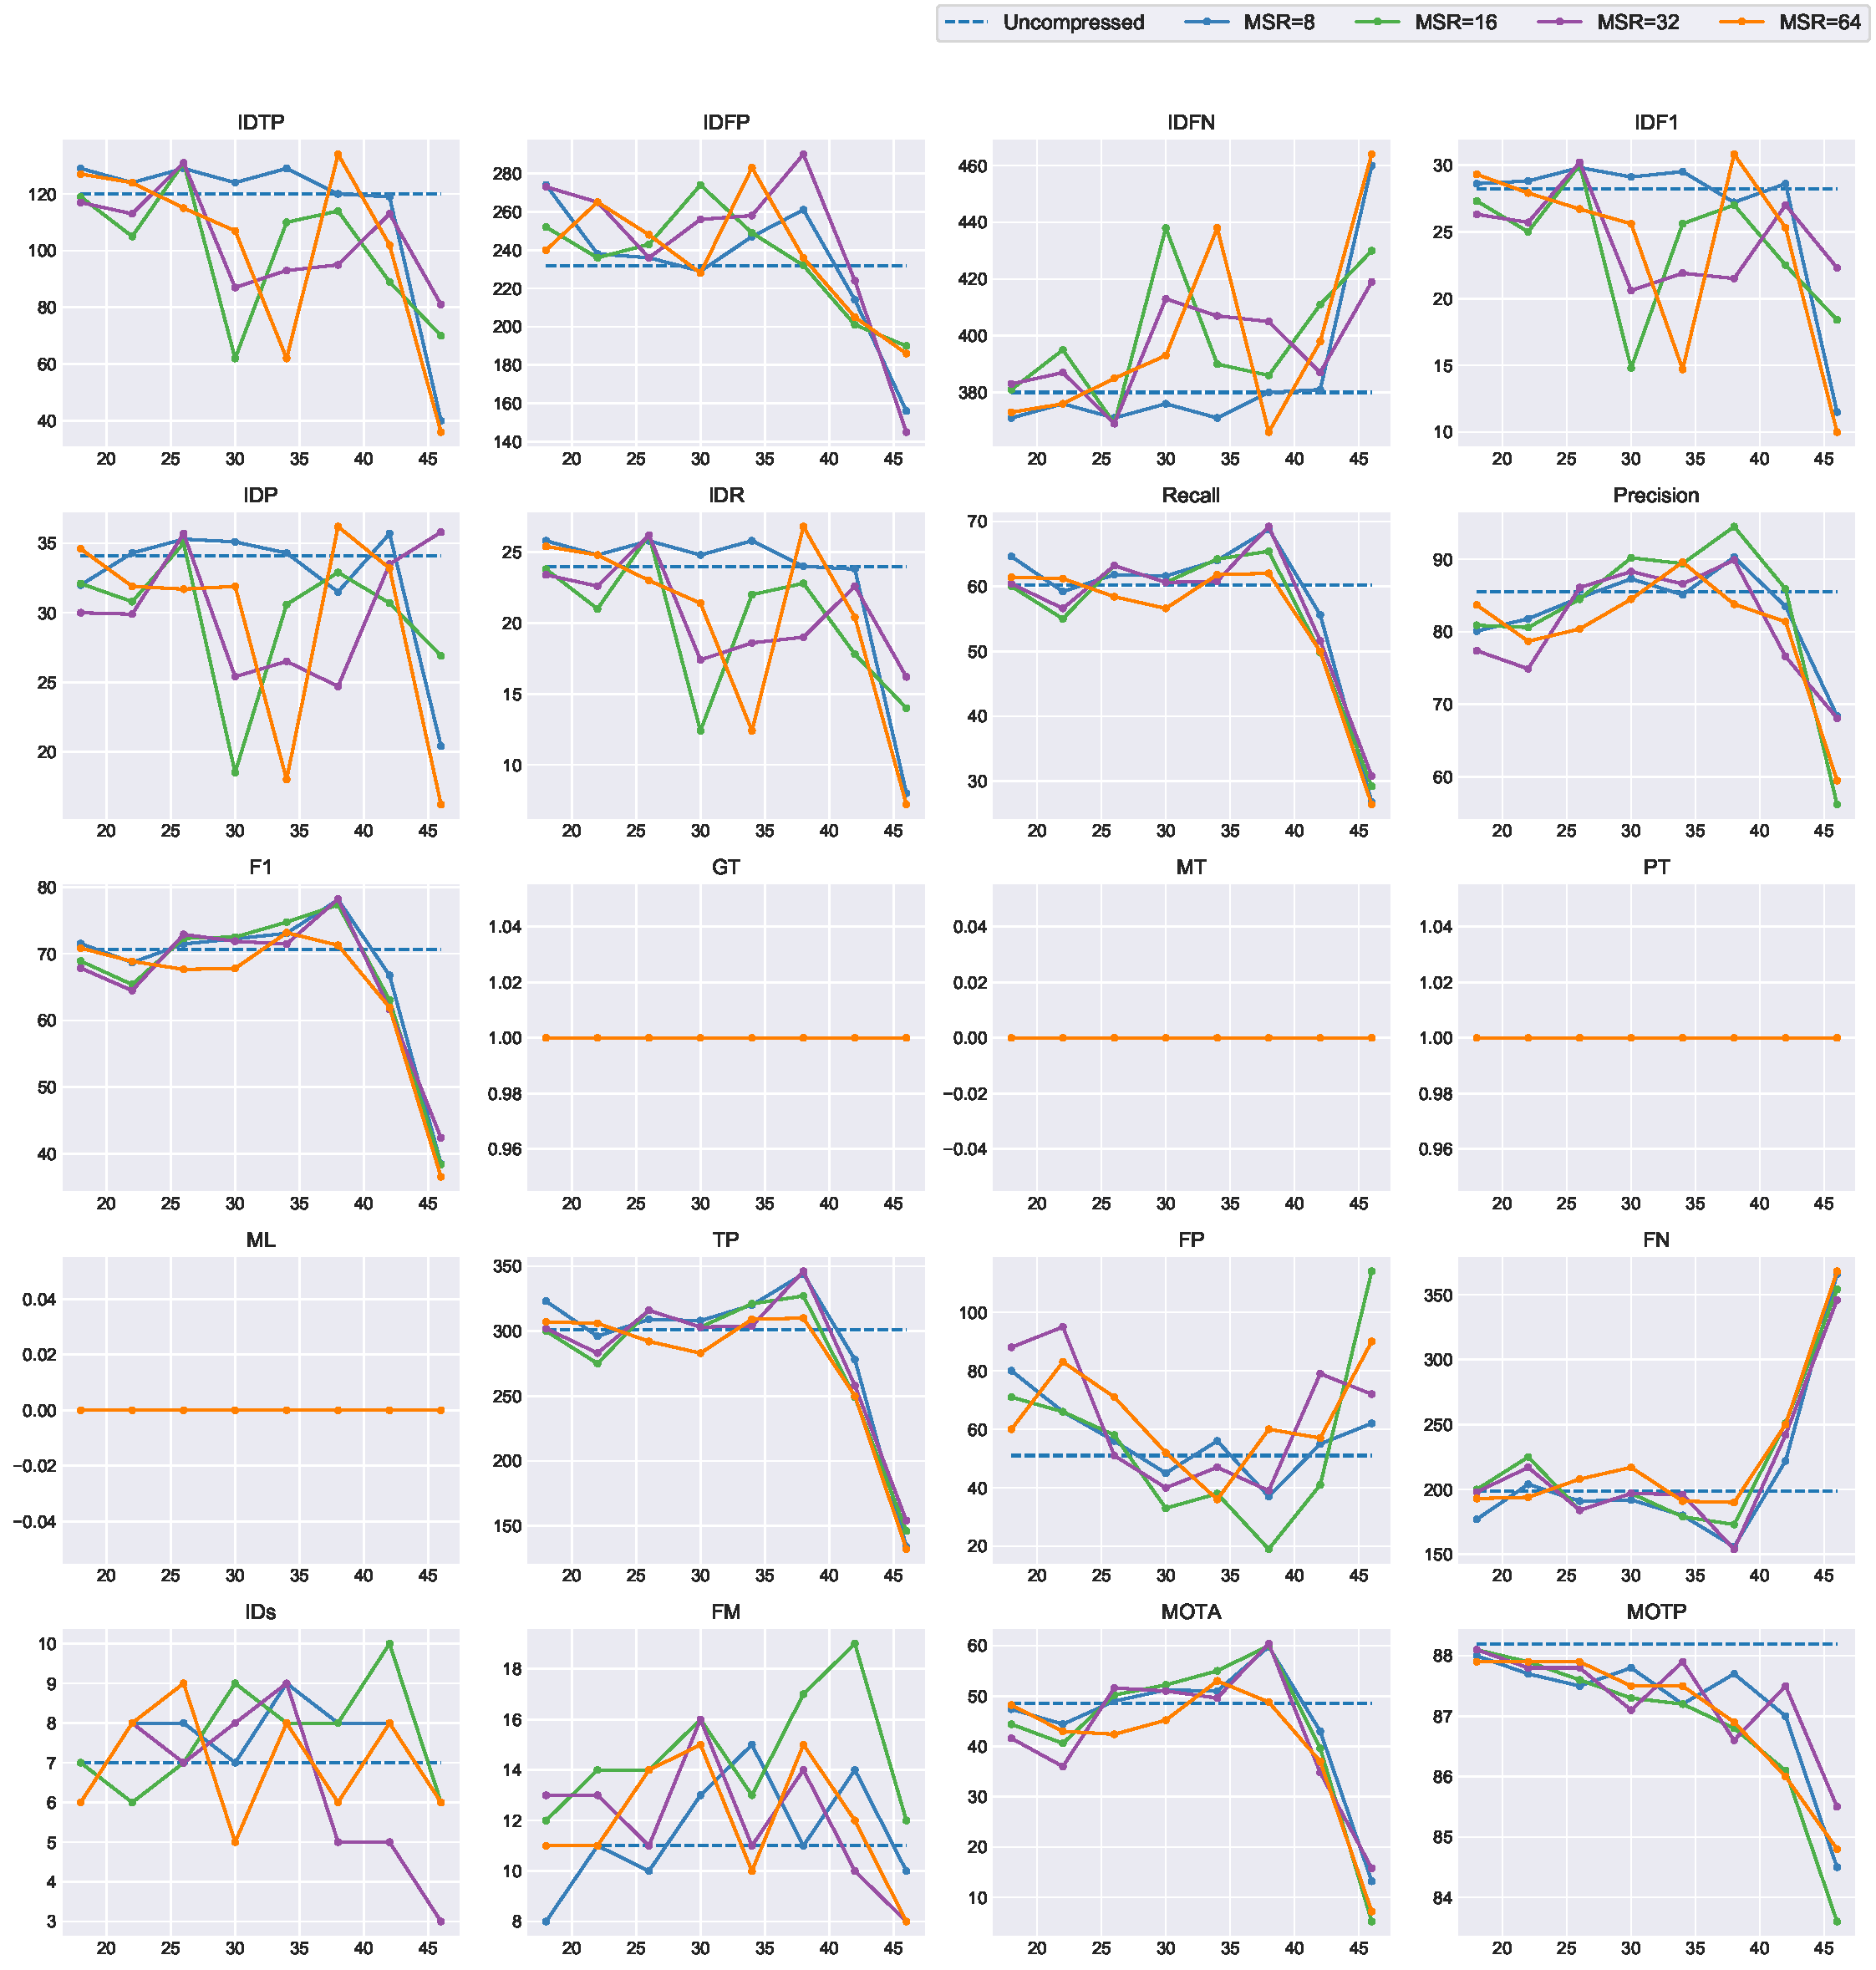
\includegraphics[width=1.0\linewidth]{img/appendix/Cactus_all_multiplots_qp.pdf}
\caption[Result of all object classes in Class B Cactus with Horizontal Axis of QP]{}
\label{fig:Cactus_all_qp}
\end{figure}

\begin{figure}[!htbp]
\centering
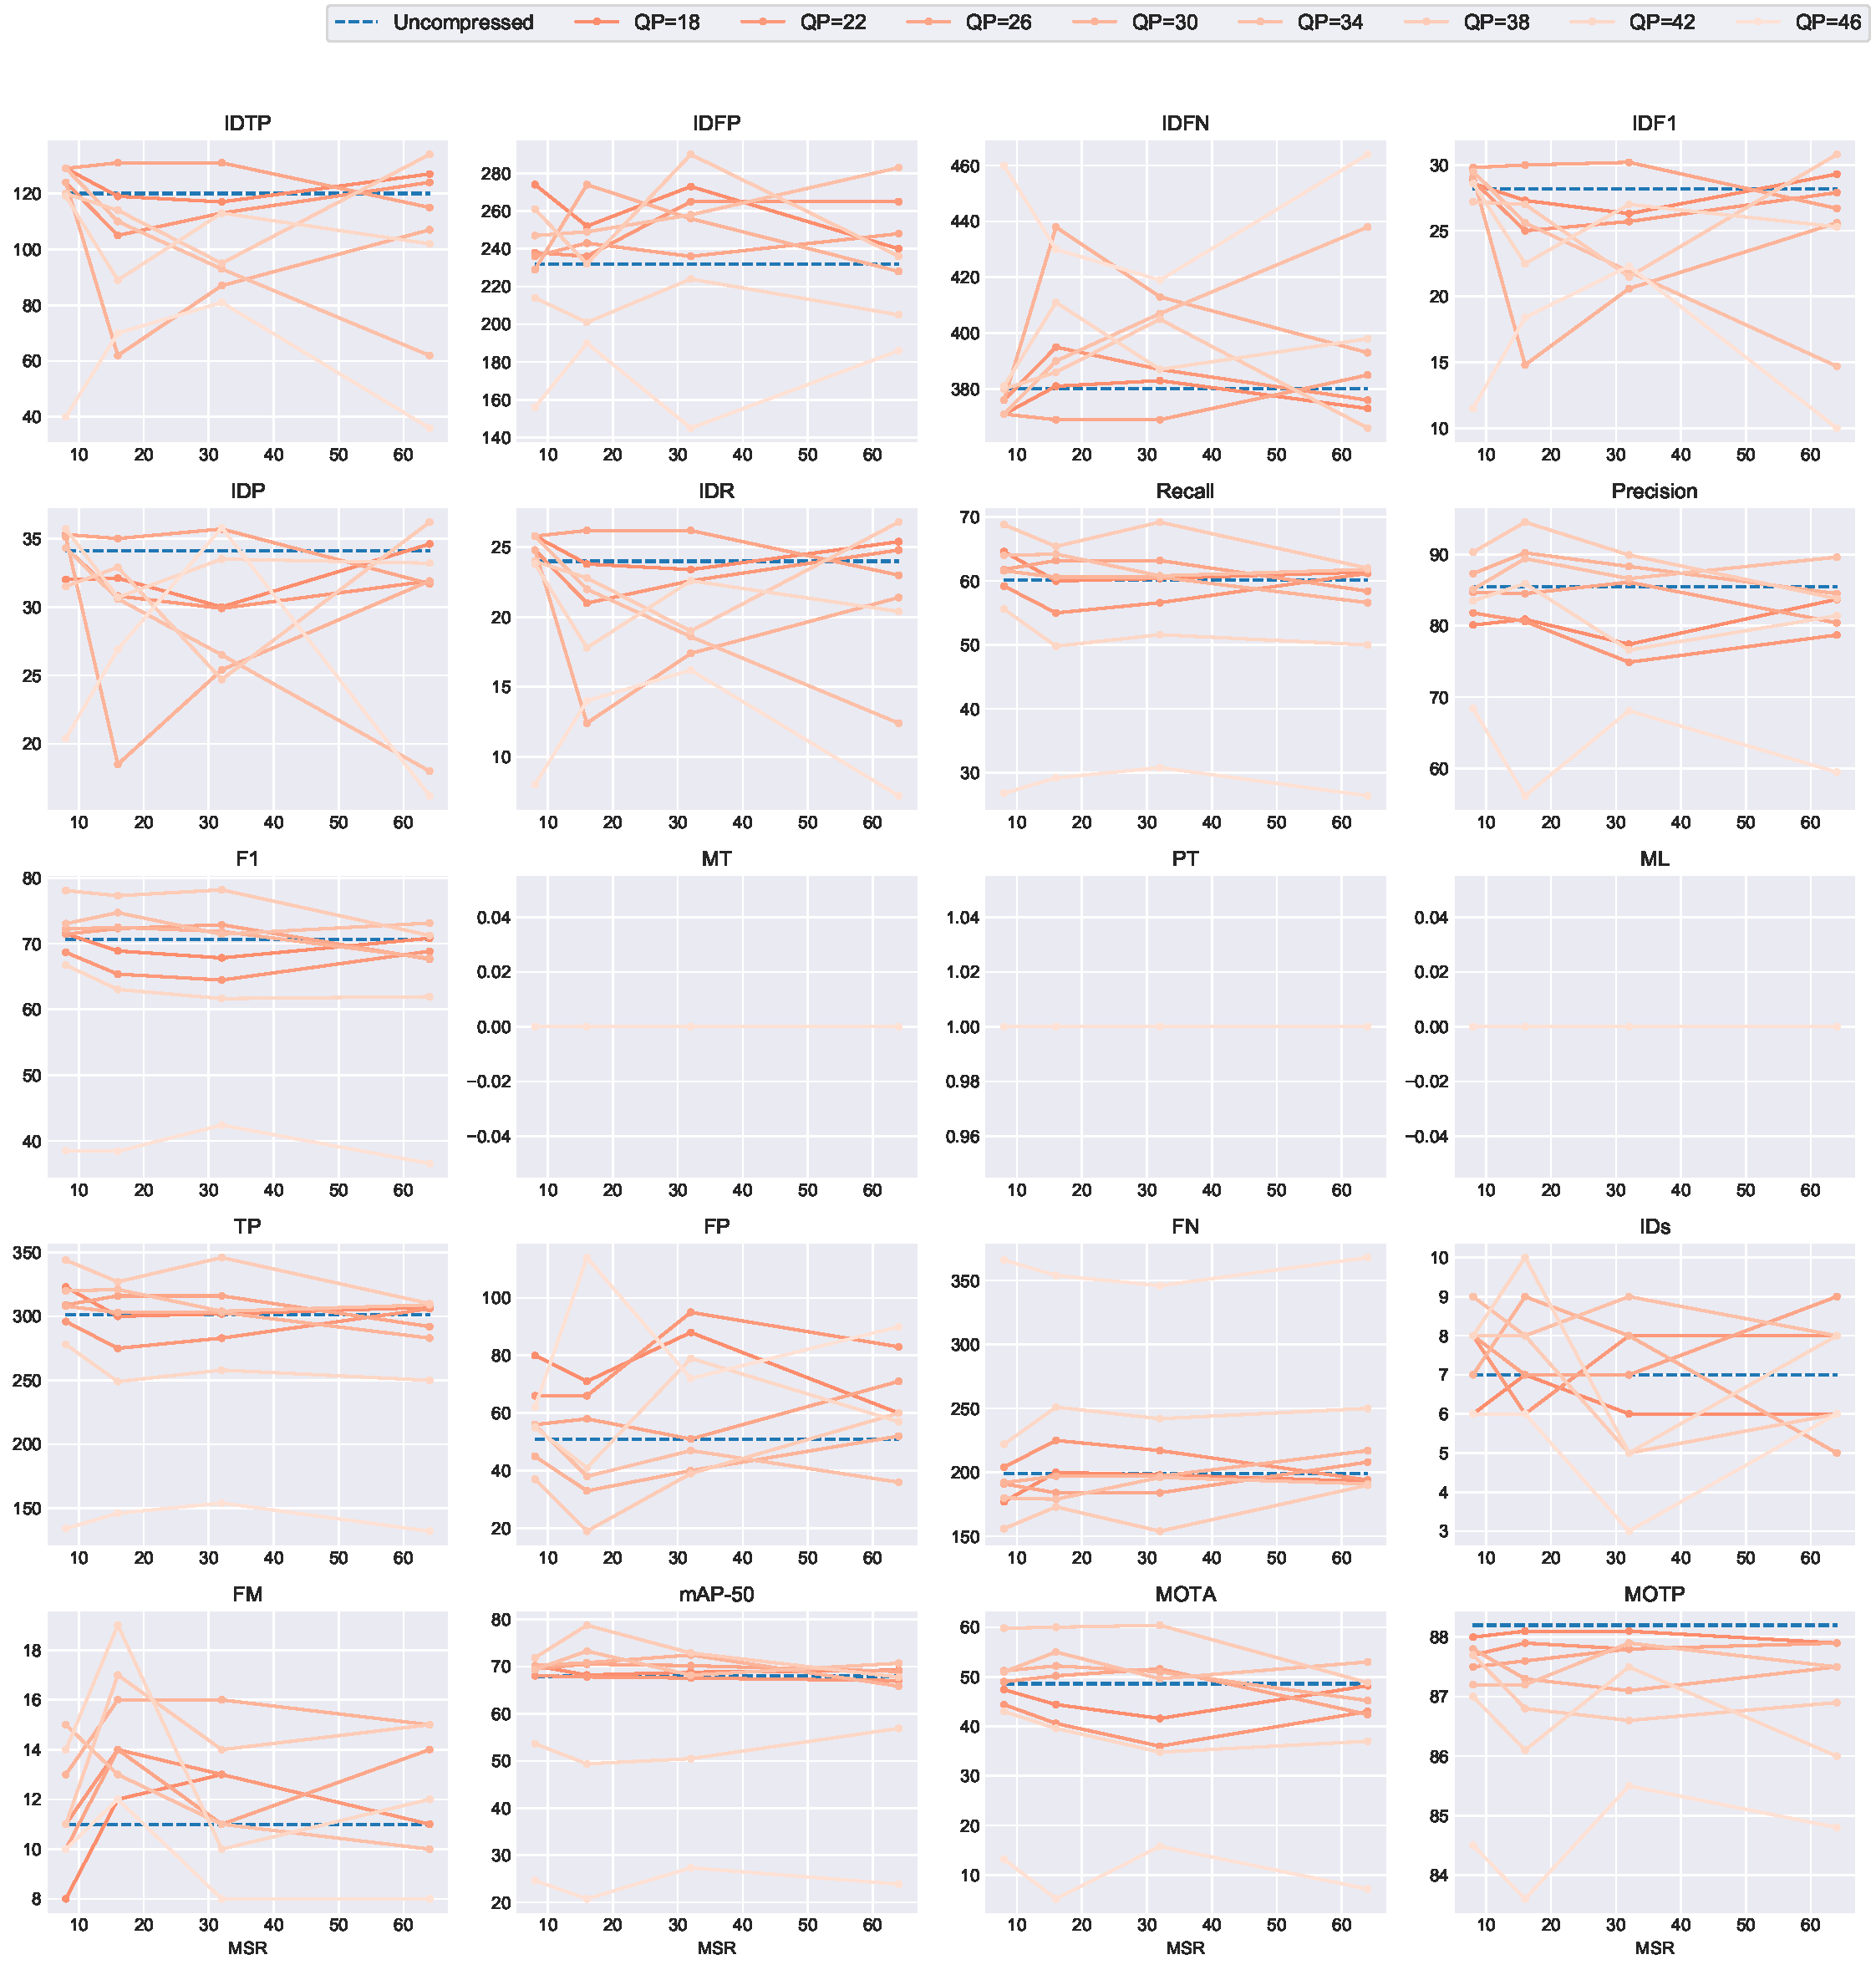
\includegraphics[width=1.0\linewidth]{img/appendix/Cactus_all_multiplots_msr.pdf}
\caption[Result of all object classes in Class B Cactus with Horizontal Axis of MSR]{}
\label{fig:Cactus_all_msr}
\end{figure}



% table
\begin{table}
\centering
\caption{Result of all object classes in Class B Cactus}


% table for uncompressed
\begin{subtable}[t]{\linewidth}
\centering
\vspace{0pt}
\resizebox{1.0\linewidth}{!}{
\begin{tabular}{llrrrrrrrrrrrrrrrrrrrr}
\toprule
          QP &          MSR &   IDTP &   IDFP &   IDFN &  IDF1 &   IDP &   IDR &  Recall &  Precision &    F1 &  GT &  MT &  PT &  ML &  TP &  FP &  FN &  IDs &  FM &  MOTA &  MOTP \\
\midrule
Uncompressed & Uncompressed & 120.00 & 232.00 & 380.00 & 28.20 & 34.10 & 24.00 &   60.20 &      85.50 & 70.65 &   1 &   0 &   1 &   0 & 301 &  51 & 199 &    7 &  11 & 48.60 & 88.20 \\
\bottomrule
\end{tabular}

}
\caption{Uncompressed Sequence}
\end{subtable}


% table for msr=8
\begin{subtable}[t]{\linewidth}
\centering
\resizebox{1.0\linewidth}{!}{
\begin{tabular}{rrrrrrrrrrrrrrrrrrrrrr}
\toprule
 QP &  MSR &   IDTP &   IDFP &   IDFN &  IDF1 &   IDP &   IDR &  Recall &  Precision &    F1 &  GT &  MT &  PT &  ML &  TP &  FP &  FN &  IDs &  FM &  MOTA &  MOTP \\
\midrule
 18 &    8 & 129.00 & 274.00 & 371.00 & 28.60 & 32.00 & 25.80 &   64.60 &      80.10 & 71.52 &   1 &   0 &   1 &   0 & 323 &  80 & 177 &    6 &   8 & 47.40 & 88.00 \\
 22 &    8 & 124.00 & 238.00 & 376.00 & 28.80 & 34.30 & 24.80 &   59.20 &      81.80 & 68.69 &   1 &   0 &   1 &   0 & 296 &  66 & 204 &    8 &  11 & 44.40 & 87.70 \\
 26 &    8 & 129.00 & 236.00 & 371.00 & 29.80 & 35.30 & 25.80 &   61.80 &      84.70 & 71.46 &   1 &   0 &   1 &   0 & 309 &  56 & 191 &    8 &  10 & 49.00 & 87.50 \\
 30 &    8 & 124.00 & 229.00 & 376.00 & 29.10 & 35.10 & 24.80 &   61.60 &      87.30 & 72.23 &   1 &   0 &   1 &   0 & 308 &  45 & 192 &    7 &  13 & 51.20 & 87.80 \\
 34 &    8 & 129.00 & 247.00 & 371.00 & 29.50 & 34.30 & 25.80 &   64.00 &      85.10 & 73.06 &   1 &   0 &   1 &   0 & 320 &  56 & 180 &    9 &  15 & 51.00 & 87.20 \\
 38 &    8 & 120.00 & 261.00 & 380.00 & 27.20 & 31.50 & 24.00 &   68.80 &      90.30 & 78.10 &   1 &   0 &   1 &   0 & 344 &  37 & 156 &    8 &  11 & 59.80 & 87.70 \\
 42 &    8 & 119.00 & 214.00 & 381.00 & 28.60 & 35.70 & 23.80 &   55.60 &      83.50 & 66.75 &   1 &   0 &   1 &   0 & 278 &  55 & 222 &    8 &  14 & 43.00 & 87.00 \\
 46 &    8 &  40.00 & 156.00 & 460.00 & 11.50 & 20.40 &  8.00 &   26.80 &      68.40 & 38.51 &   1 &   0 &   1 &   0 & 134 &  62 & 366 &    6 &  10 & 13.20 & 84.50 \\
\bottomrule
\end{tabular}

}
\caption{MSR = 8}
\end{subtable}



% table for msr=16
\begin{subtable}[t]{\linewidth}
\centering
\resizebox{1.0\linewidth}{!}{
\begin{tabular}{rrrrrrrrrrrrrrrrrrrrrr}
\toprule
 QP &  MSR &   IDTP &   IDFP &   IDFN &  IDF1 &   IDP &   IDR &  Recall &  Precision &    F1 &  GT &  MT &  PT &  ML &  TP &  FP &  FN &  IDs &  FM &  MOTA &  MOTP \\
\midrule
 18 &   16 & 119.00 & 252.00 & 381.00 & 27.30 & 32.10 & 23.80 &   60.00 &      80.90 & 68.90 &   1 &   0 &   1 &   0 & 300 &  71 & 200 &    7 &  12 & 44.40 & 88.10 \\
 22 &   16 & 105.00 & 236.00 & 395.00 & 25.00 & 30.80 & 21.00 &   55.00 &      80.60 & 65.38 &   1 &   0 &   1 &   0 & 275 &  66 & 225 &    6 &  14 & 40.60 & 87.90 \\
 26 &   16 & 131.00 & 243.00 & 369.00 & 30.00 & 35.00 & 26.20 &   63.20 &      84.50 & 72.31 &   1 &   0 &   1 &   0 & 316 &  58 & 184 &    7 &  14 & 50.20 & 87.60 \\
 30 &   16 &  62.00 & 274.00 & 438.00 & 14.80 & 18.50 & 12.40 &   60.60 &      90.20 & 72.49 &   1 &   0 &   1 &   0 & 303 &  33 & 197 &    9 &  16 & 52.20 & 87.30 \\
 34 &   16 & 110.00 & 249.00 & 390.00 & 25.60 & 30.60 & 22.00 &   64.20 &      89.40 & 74.73 &   1 &   0 &   1 &   0 & 321 &  38 & 179 &    8 &  13 & 55.00 & 87.20 \\
 38 &   16 & 114.00 & 232.00 & 386.00 & 27.00 & 32.90 & 22.80 &   65.40 &      94.50 & 77.30 &   1 &   0 &   1 &   0 & 327 &  19 & 173 &    8 &  17 & 60.00 & 86.80 \\
 42 &   16 &  89.00 & 201.00 & 411.00 & 22.50 & 30.70 & 17.80 &   49.80 &      85.90 & 63.05 &   1 &   0 &   1 &   0 & 249 &  41 & 251 &   10 &  19 & 39.60 & 86.10 \\
 46 &   16 &  70.00 & 190.00 & 430.00 & 18.40 & 26.90 & 14.00 &   29.20 &      56.20 & 38.43 &   1 &   0 &   1 &   0 & 146 & 114 & 354 &    6 &  12 &  5.20 & 83.60 \\
\bottomrule
\end{tabular}

}
\caption{MSR = 16}
\end{subtable}


% table for msr=32
\begin{subtable}[t]{\linewidth}
\centering
\resizebox{1.0\linewidth}{!}{
\begin{tabular}{rrrrrrrrrrrrrrrrrrrrrr}
\toprule
 QP &  MSR &   IDTP &   IDFP &   IDFN &  IDF1 &   IDP &   IDR &  Recall &  Precision &    F1 &  GT &  MT &  PT &  ML &  TP &  FP &  FN &  IDs &  FM &  MOTA &  MOTP \\
\midrule
 18 &   32 & 117.00 & 273.00 & 383.00 & 26.30 & 30.00 & 23.40 &   60.40 &      77.40 & 67.85 &   1 &   0 &   1 &   0 & 302 &  88 & 198 &    6 &  13 & 41.60 & 88.10 \\
 22 &   32 & 113.00 & 265.00 & 387.00 & 25.70 & 29.90 & 22.60 &   56.60 &      74.90 & 64.48 &   1 &   0 &   1 &   0 & 283 &  95 & 217 &    8 &  13 & 36.00 & 87.80 \\
 26 &   32 & 131.00 & 236.00 & 369.00 & 30.20 & 35.70 & 26.20 &   63.20 &      86.10 & 72.89 &   1 &   0 &   1 &   0 & 316 &  51 & 184 &    7 &  11 & 51.60 & 87.80 \\
 30 &   32 &  87.00 & 256.00 & 413.00 & 20.60 & 25.40 & 17.40 &   60.60 &      88.30 & 71.87 &   1 &   0 &   1 &   0 & 303 &  40 & 197 &    8 &  16 & 51.00 & 87.10 \\
 34 &   32 &  93.00 & 258.00 & 407.00 & 21.90 & 26.50 & 18.60 &   60.80 &      86.60 & 71.44 &   1 &   0 &   1 &   0 & 304 &  47 & 196 &    9 &  11 & 49.60 & 87.90 \\
 38 &   32 &  95.00 & 290.00 & 405.00 & 21.50 & 24.70 & 19.00 &   69.20 &      89.90 & 78.20 &   1 &   0 &   1 &   0 & 346 &  39 & 154 &    5 &  14 & 60.40 & 86.60 \\
 42 &   32 & 113.00 & 224.00 & 387.00 & 27.00 & 33.50 & 22.60 &   51.60 &      76.60 & 61.66 &   1 &   0 &   1 &   0 & 258 &  79 & 242 &    5 &  10 & 34.80 & 87.50 \\
 46 &   32 &  81.00 & 145.00 & 419.00 & 22.30 & 35.80 & 16.20 &   30.80 &      68.10 & 42.42 &   1 &   0 &   1 &   0 & 154 &  72 & 346 &    3 &   8 & 15.80 & 85.50 \\
\bottomrule
\end{tabular}

}
\caption{MSR = 32}
\end{subtable}


% table for msr=64
\begin{subtable}[t]{\linewidth}
\centering
\resizebox{1.0\linewidth}{!}{
\begin{tabular}{rrrrrrrrrrrrrrrrrrrrrr}
\toprule
 QP &  MSR &   IDTP &   IDFP &   IDFN &  IDF1 &   IDP &   IDR &  Recall &  Precision &    F1 &  GT &  MT &  PT &  ML &  TP &  FP &  FN &  IDs &  FM &  MOTA &  MOTP \\
\midrule
 18 &   64 & 127.00 & 240.00 & 373.00 & 29.30 & 34.60 & 25.40 &   61.40 &      83.70 & 70.84 &   1 &   0 &   1 &   0 & 307 &  60 & 193 &    6 &  11 & 48.20 & 87.90 \\
 22 &   64 & 124.00 & 265.00 & 376.00 & 27.90 & 31.90 & 24.80 &   61.20 &      78.70 & 68.86 &   1 &   0 &   1 &   0 & 306 &  83 & 194 &    8 &  11 & 43.00 & 87.90 \\
 26 &   64 & 115.00 & 248.00 & 385.00 & 26.70 & 31.70 & 23.00 &   58.40 &      80.40 & 67.66 &   1 &   0 &   1 &   0 & 292 &  71 & 208 &    9 &  14 & 42.40 & 87.90 \\
 30 &   64 & 107.00 & 228.00 & 393.00 & 25.60 & 31.90 & 21.40 &   56.60 &      84.50 & 67.79 &   1 &   0 &   1 &   0 & 283 &  52 & 217 &    5 &  15 & 45.20 & 87.50 \\
 34 &   64 &  62.00 & 283.00 & 438.00 & 14.70 & 18.00 & 12.40 &   61.80 &      89.60 & 73.15 &   1 &   0 &   1 &   0 & 309 &  36 & 191 &    8 &  10 & 53.00 & 87.50 \\
 38 &   64 & 134.00 & 236.00 & 366.00 & 30.80 & 36.20 & 26.80 &   62.00 &      83.80 & 71.27 &   1 &   0 &   1 &   0 & 310 &  60 & 190 &    6 &  15 & 48.80 & 86.90 \\
 42 &   64 & 102.00 & 205.00 & 398.00 & 25.30 & 33.20 & 20.40 &   50.00 &      81.40 & 61.95 &   1 &   0 &   1 &   0 & 250 &  57 & 250 &    8 &  12 & 37.00 & 86.00 \\
 46 &   64 &  36.00 & 186.00 & 464.00 & 10.00 & 16.20 &  7.20 &   26.40 &      59.50 & 36.57 &   1 &   0 &   1 &   0 & 132 &  90 & 368 &    6 &   8 &  7.20 & 84.80 \\
\bottomrule
\end{tabular}

}
\caption{MSR = 64}
\end{subtable}


\label{tab:Cactus_all}
\end{table}




\begin{table}[!htbp]
\centering
\caption{Multiple Linear Regression Analysis Result for Class B Cactus}
\resizebox{1.0\linewidth}{!}{
\begin{tabular}{lrrrrrrrrrrrrrrrrrrr}
\toprule
{} &   IDTP &   IDFP &   IDFN &  IDF1 &   IDP &   IDR &  Recall &  Precision &    F1 &   MT &    PT &   ML &     TP &    FP &     FN &   IDs &    FM &  MOTA &  MOTP \\
\midrule
coefficient(Intercept) & 153.49 & 314.45 & 346.51 & 33.14 & 33.86 & 30.70 &   79.32 &      88.74 & 86.06 & 0.00 &  1.00 & 0.00 & 396.62 & 71.32 & 103.38 &  7.34 & 10.00 & 63.59 & 90.13 \\
coefficient(QP)        &  -1.38 &  -2.50 &   1.38 & -0.23 & -0.07 & -0.28 &   -0.68 &      -0.18 & -0.57 & 0.00 & -0.00 & 0.00 &  -3.40 & -0.49 &   3.40 &  0.00 &  0.09 & -0.58 & -0.10 \\
coefficient(MSR)       &   0.11 &  -0.12 &  -0.11 &  0.03 &  0.05 &  0.02 &    0.02 &       0.05 &  0.03 & 0.00 & -0.00 & 0.00 &   0.09 & -0.10 &  -0.09 &  0.02 &  0.08 &  0.03 & -0.00 \\
coefficient(QP*MSR)    &  -0.01 &   0.01 &   0.01 & -0.00 & -0.00 & -0.00 &   -0.00 &      -0.00 & -0.00 & 0.00 &  0.00 & 0.00 &  -0.01 &  0.01 &   0.01 & -0.00 & -0.00 & -0.00 &  0.00 \\
p-value(Intercept)     &   0.00 &   0.00 &   0.00 &  0.00 &  0.00 &  0.00 &    0.00 &       0.00 &  0.00 &  NaN &  0.00 &  NaN &   0.00 &  0.01 &   0.07 &  0.00 &  0.00 &  0.00 &  0.00 \\
p-value(QP)            &   0.08 &   0.01 &   0.08 &  0.17 &  0.70 &  0.08 &    0.05 &       0.54 &  0.10 &  NaN &  0.11 &  NaN &   0.05 &  0.49 &   0.05 &  0.94 &  0.31 &  0.19 &  0.00 \\
p-value(MSR)           &   0.87 &   0.88 &   0.87 &  0.84 &  0.75 &  0.87 &    0.95 &       0.84 &  0.93 &  NaN &  0.14 &  NaN &   0.95 &  0.88 &   0.95 &  0.72 &  0.31 &  0.93 &  1.00 \\
p-value(QP*MSR)        &   0.69 &   0.80 &   0.69 &  0.66 &  0.57 &  0.69 &    0.83 &       0.69 &  0.81 &  NaN &  0.62 &  NaN &   0.83 &  0.70 &   0.83 &  0.54 &  0.22 &  0.79 &  0.98 \\
\bottomrule
\end{tabular}

}
\label{tab:Cactus_all_reg}
\end{table}



\newpage

\section{Kimono}
\label{sec:appendix/Kimono_all}


% visualization figure
\begin{figure}[!htbp]
\centering
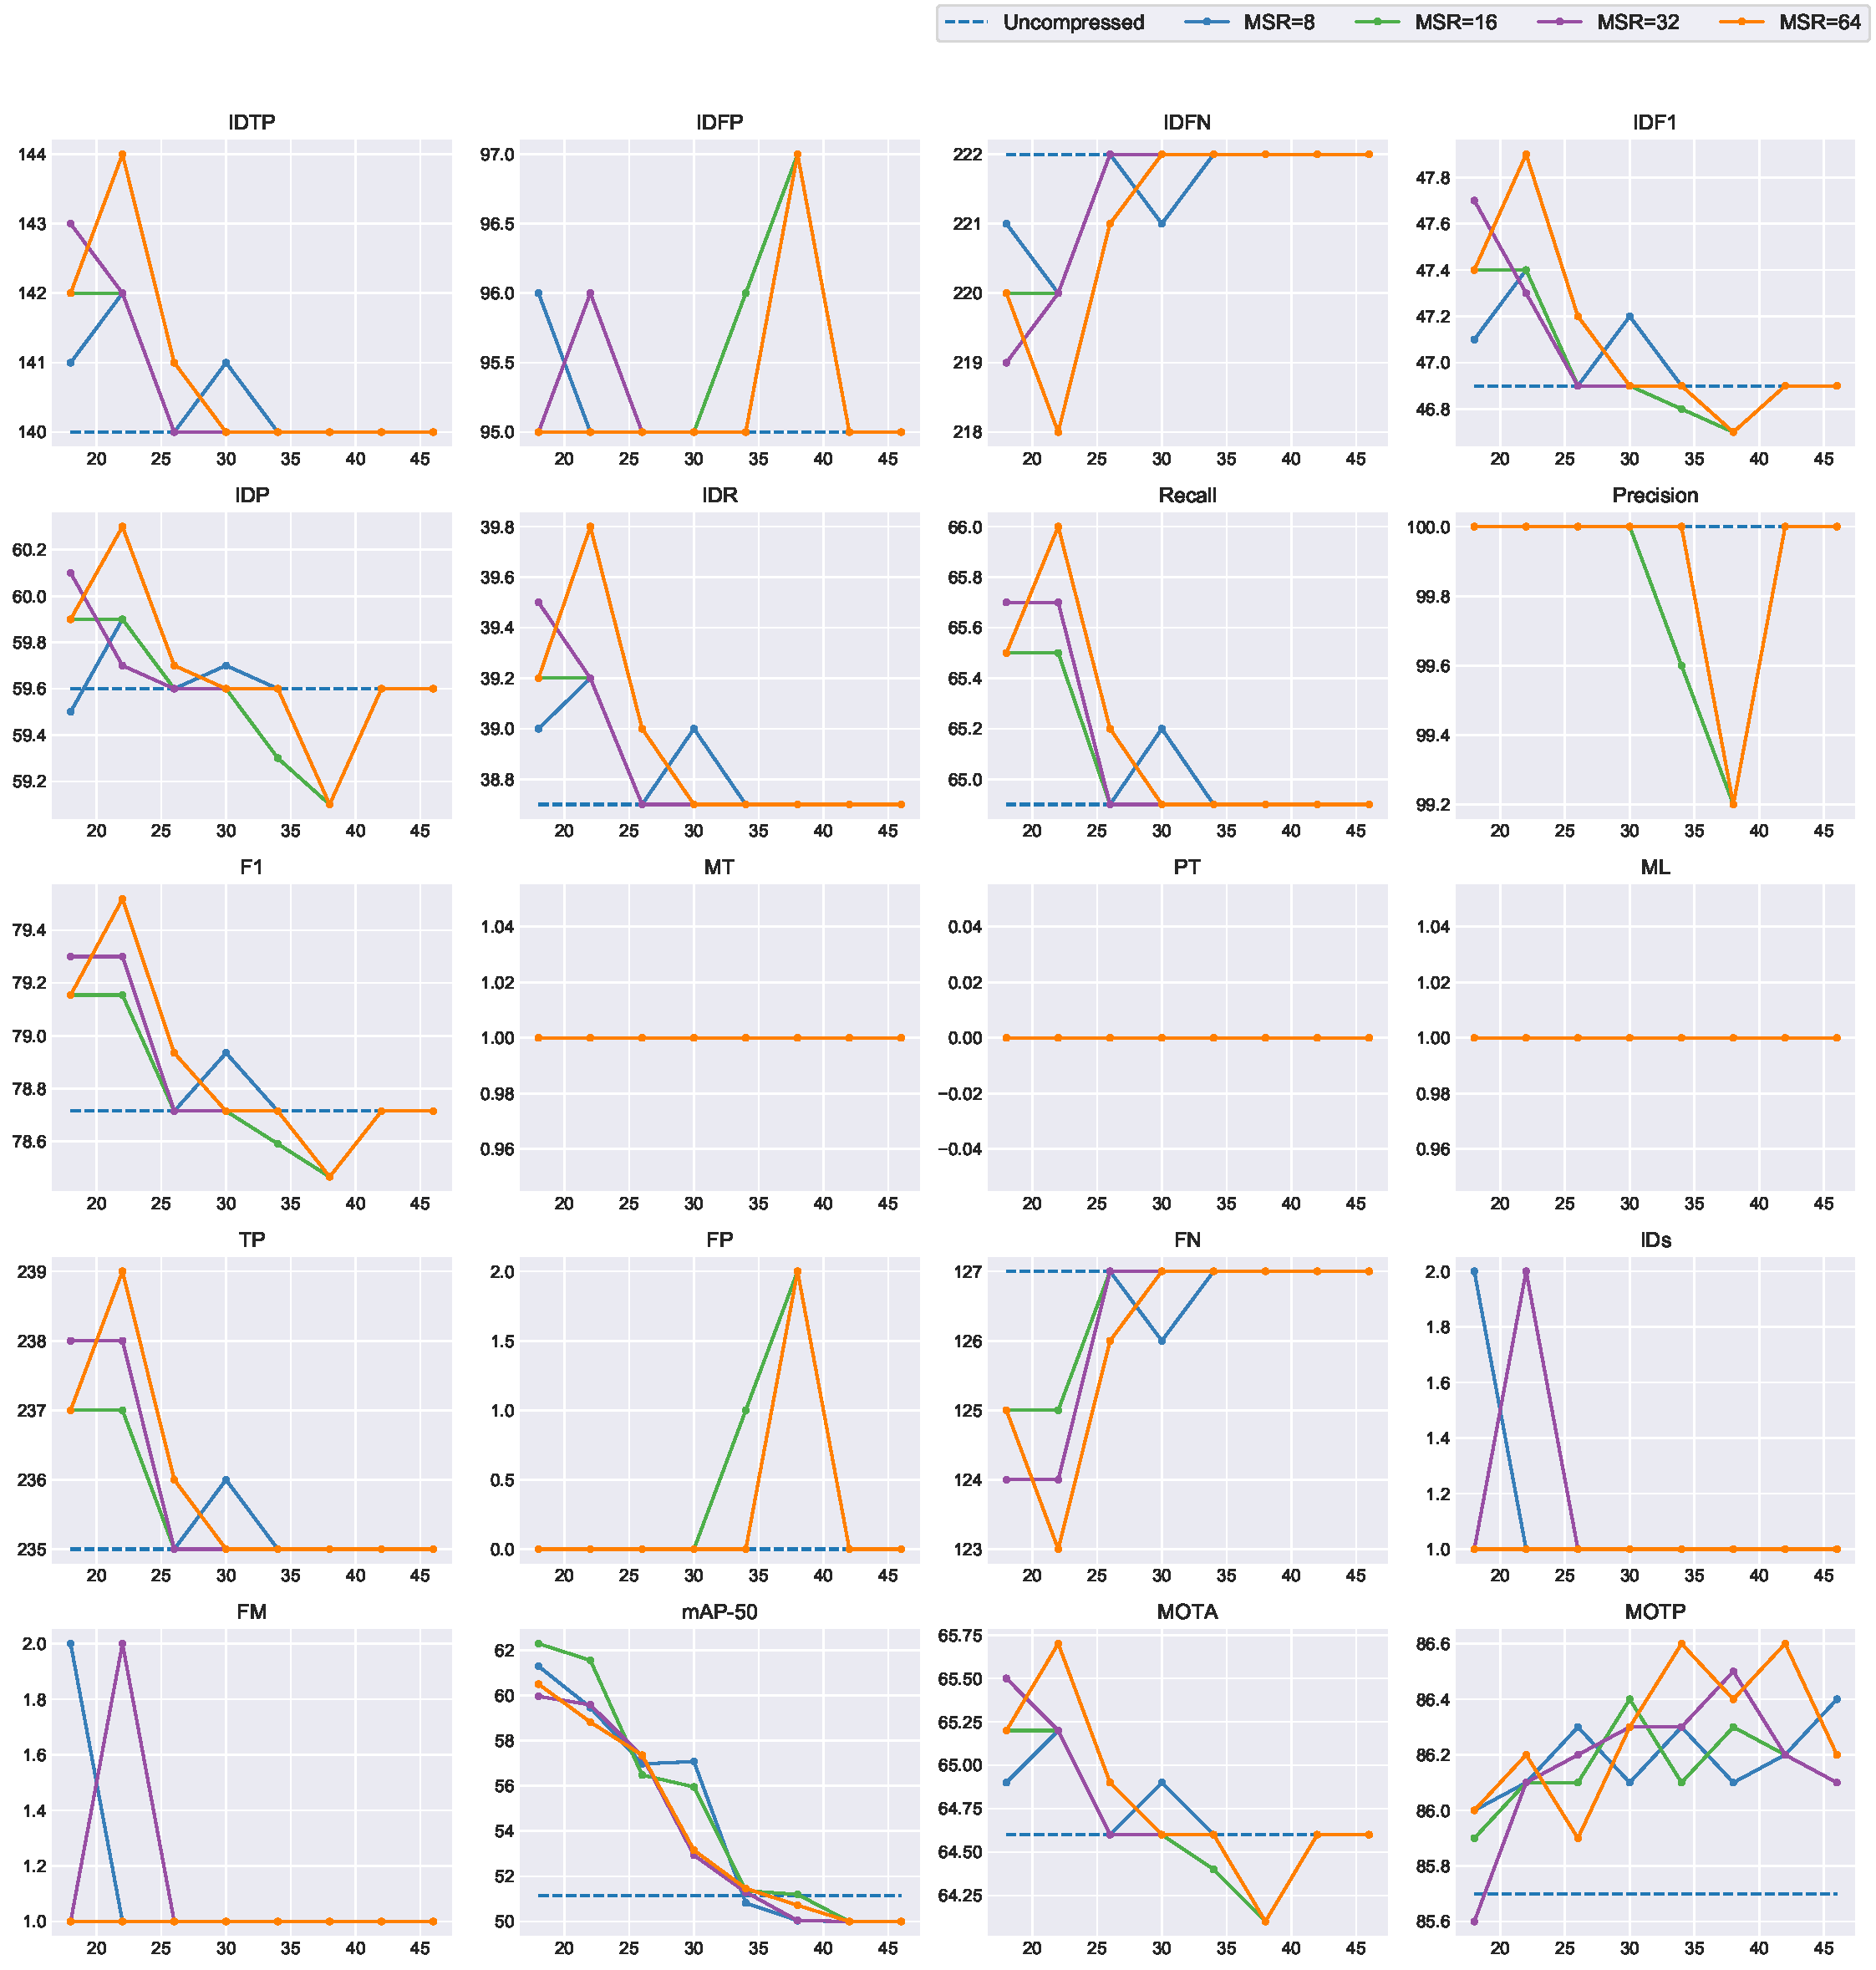
\includegraphics[width=1.0\linewidth]{img/appendix/Kimono_all_multiplots_qp.pdf}
\caption[Visualization of performance results on Kimono at different QP]
{Visualization of performance results on Kimono at different QP.}
\label{fig:Kimono_all_qp}
\end{figure}

\begin{figure}[!htbp]
\centering
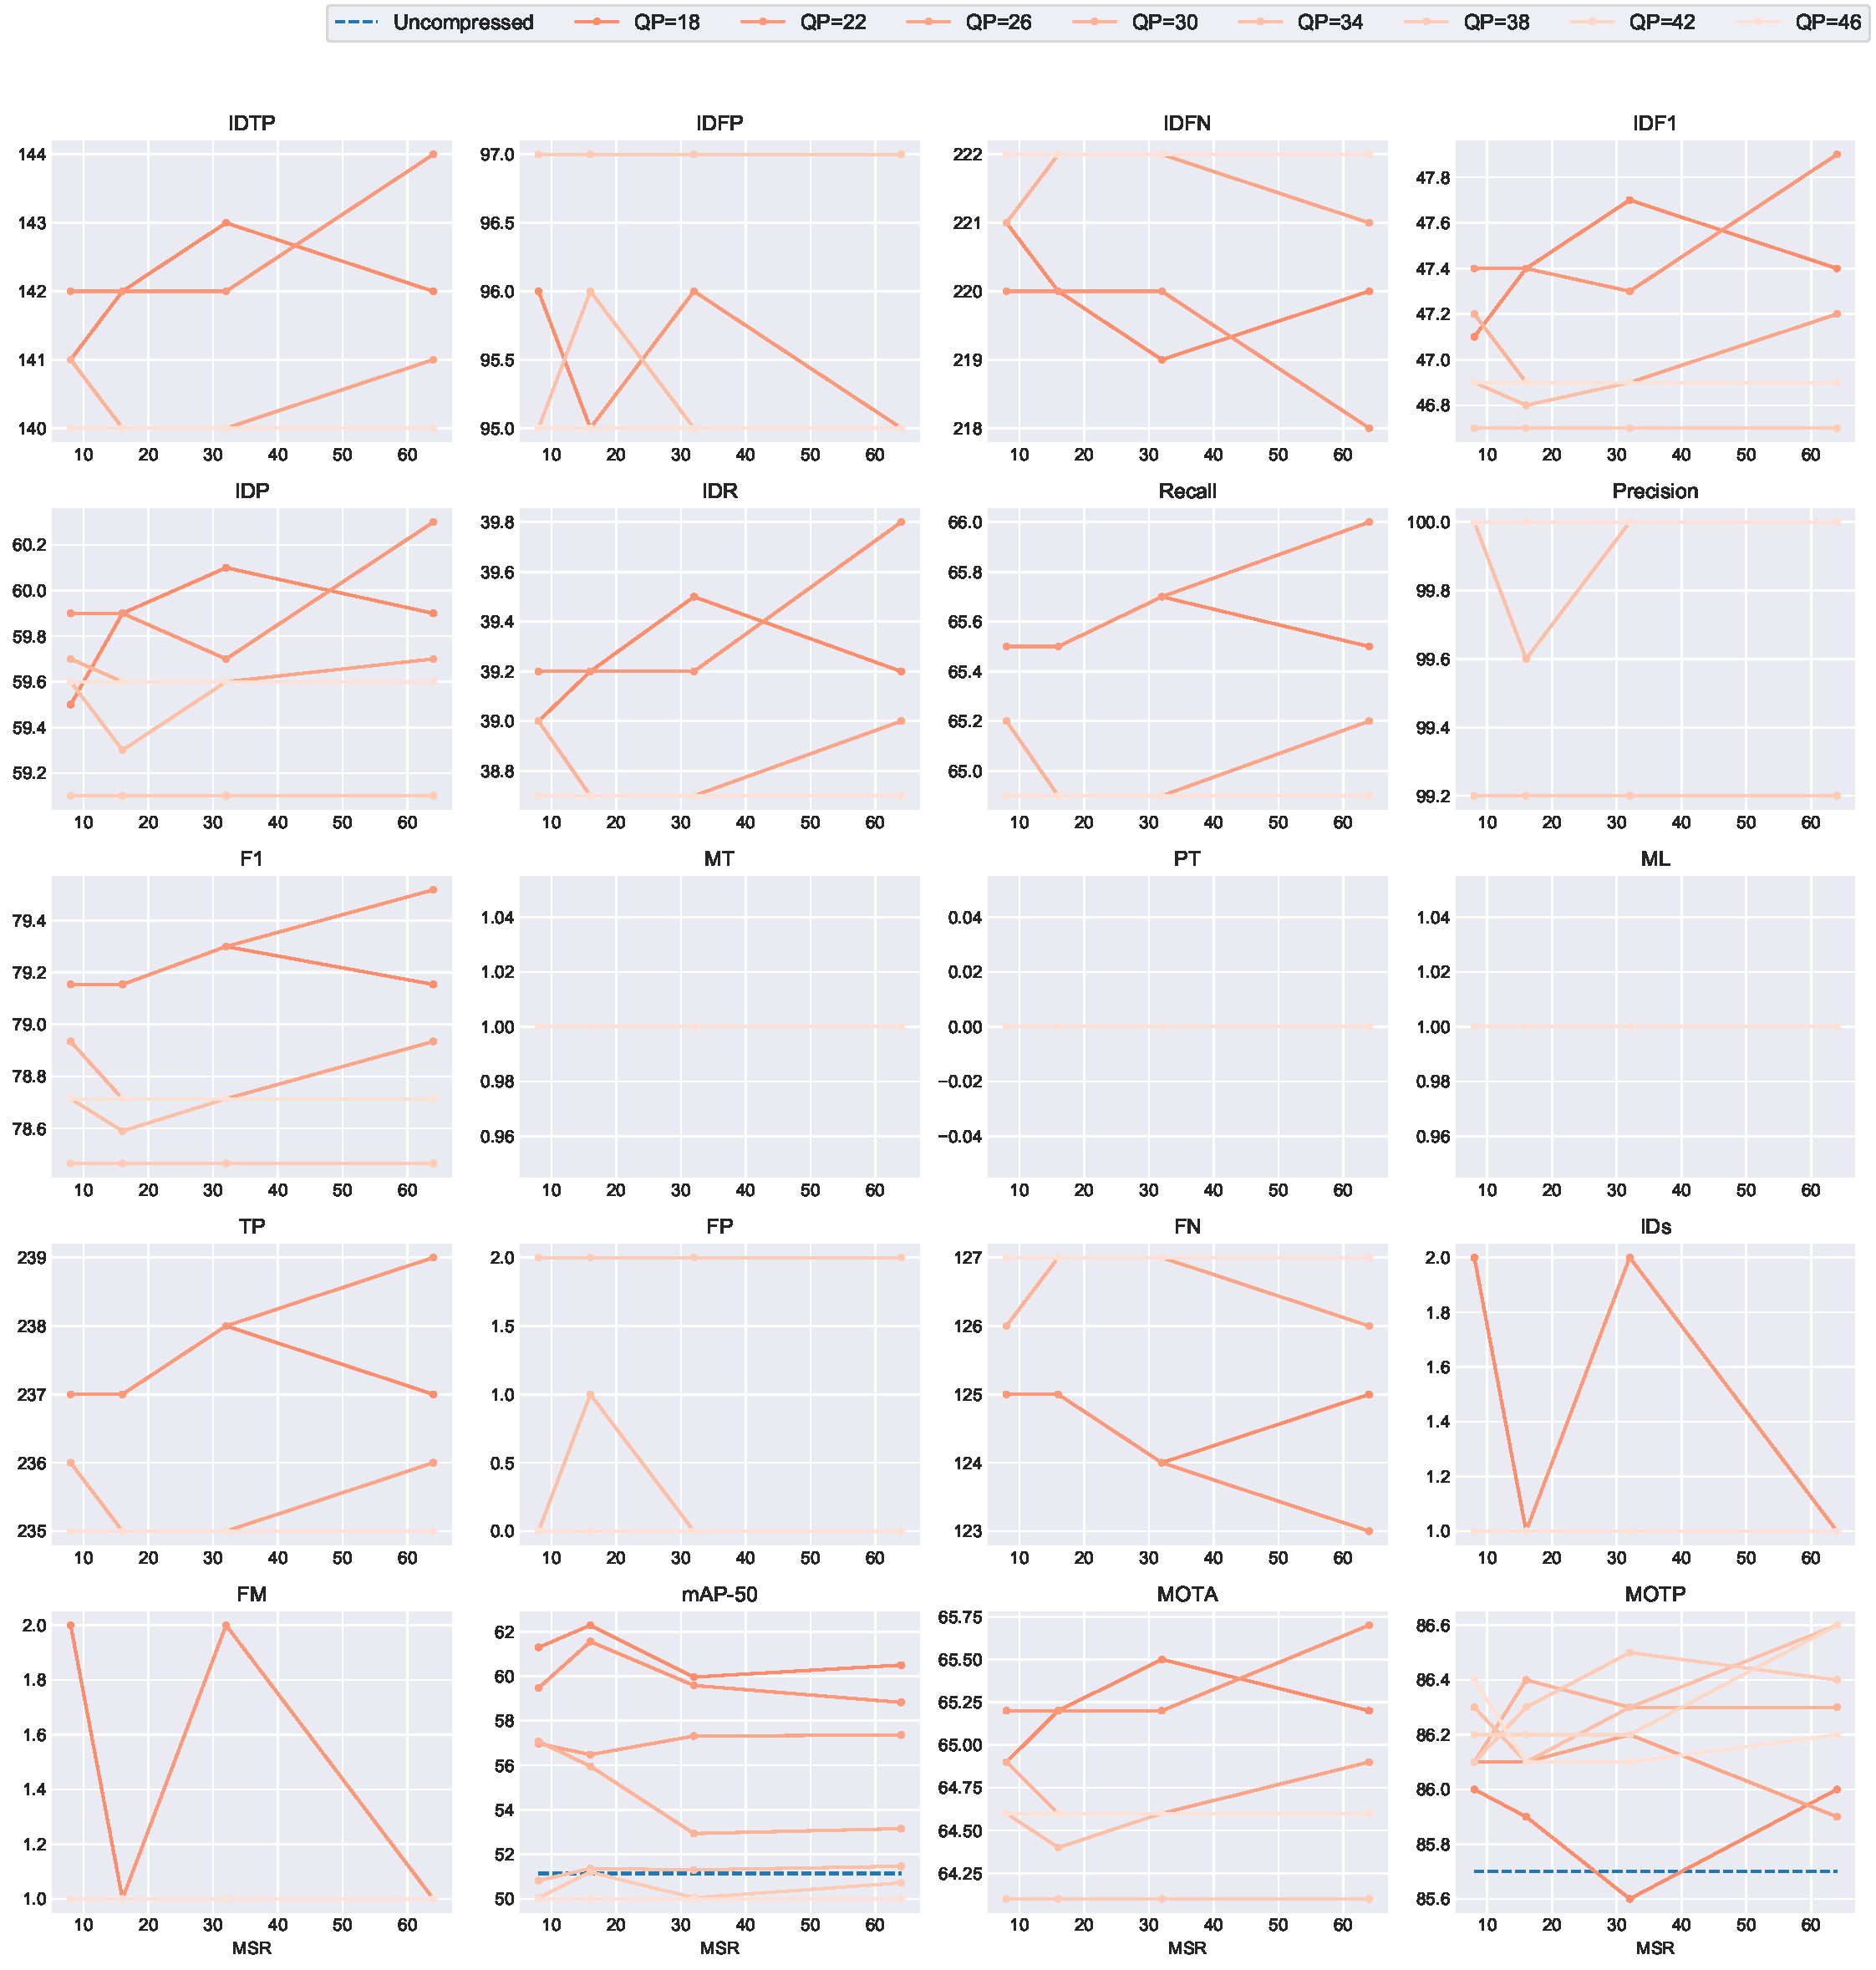
\includegraphics[width=1.0\linewidth]{img/appendix/Kimono_all_multiplots_msr.pdf}
\caption[Visualization of performance results on Kimono at different MSR]
{Visualization of performance results on Kimono at different MSR.}
\label{fig:Kimono_all_msr}
\end{figure}



% table
\begin{table}
\centering
\caption[Performance results on Kimono]
{Performance results on Kimono.}


% table for uncompressed
\begin{subtable}[t]{\linewidth}
\centering
\vspace{0pt}
\resizebox{1.0\linewidth}{!}{
\begin{tabular}{llrrrrrrrrrrrrrrrrrrrrr}
\toprule
          QP &          MSR &   IDTP &  IDFP &   IDFN &  IDF1 &   IDP &   IDR &  Recall &  Precision &    F1 &  GT &  MT &  PT &  ML &  TP &  FP &  FN &  IDs &  FM &  mAP-50 &  MOTA &  MOTP \\
\midrule
Uncompressed & Uncompressed & 140.00 & 95.00 & 222.00 & 46.90 & 59.60 & 38.70 &   64.90 &     100.00 & 78.71 &   2 &   1 &   0 &   1 & 235 &   0 & 127 &    1 &   1 &   51.14 & 64.60 & 85.70 \\
\bottomrule
\end{tabular}

}
\caption{Uncompressed Sequence}
\end{subtable}


% table for msr=8
\begin{subtable}[t]{\linewidth}
\centering
\resizebox{1.0\linewidth}{!}{
\begin{tabular}{rrrrrrrrrrrrrrrrrrrrrrr}
\toprule
 QP &  MSR &   IDTP &  IDFP &   IDFN &  IDF1 &   IDP &   IDR &  Recall &  Precision &    F1 &  GT &  MT &  PT &  ML &  TP &  FP &  FN &  IDs &  FM &  mAP-50 &  MOTA &  MOTP \\
\midrule
 18 &    8 & 141.00 & 96.00 & 221.00 & 47.10 & 59.50 & 39.00 &   65.50 &     100.00 & 79.15 &   2 &   1 &   0 &   1 & 237 &   0 & 125 &    2 &   2 &   61.29 & 64.90 & 86.00 \\
 22 &    8 & 142.00 & 95.00 & 220.00 & 47.40 & 59.90 & 39.20 &   65.50 &     100.00 & 79.15 &   2 &   1 &   0 &   1 & 237 &   0 & 125 &    1 &   1 &   59.47 & 65.20 & 86.10 \\
 26 &    8 & 140.00 & 95.00 & 222.00 & 46.90 & 59.60 & 38.70 &   64.90 &     100.00 & 78.71 &   2 &   1 &   0 &   1 & 235 &   0 & 127 &    1 &   1 &   56.97 & 64.60 & 86.30 \\
 30 &    8 & 141.00 & 95.00 & 221.00 & 47.20 & 59.70 & 39.00 &   65.20 &     100.00 & 78.93 &   2 &   1 &   0 &   1 & 236 &   0 & 126 &    1 &   1 &   57.08 & 64.90 & 86.10 \\
 34 &    8 & 140.00 & 95.00 & 222.00 & 46.90 & 59.60 & 38.70 &   64.90 &     100.00 & 78.71 &   2 &   1 &   0 &   1 & 235 &   0 & 127 &    1 &   1 &   50.82 & 64.60 & 86.30 \\
 38 &    8 & 140.00 & 97.00 & 222.00 & 46.70 & 59.10 & 38.70 &   64.90 &      99.20 & 78.47 &   2 &   1 &   0 &   1 & 235 &   2 & 127 &    1 &   1 &   50.04 & 64.10 & 86.10 \\
 42 &    8 & 140.00 & 95.00 & 222.00 & 46.90 & 59.60 & 38.70 &   64.90 &     100.00 & 78.71 &   2 &   1 &   0 &   1 & 235 &   0 & 127 &    1 &   1 &   50.00 & 64.60 & 86.20 \\
 46 &    8 & 140.00 & 95.00 & 222.00 & 46.90 & 59.60 & 38.70 &   64.90 &     100.00 & 78.71 &   2 &   1 &   0 &   1 & 235 &   0 & 127 &    1 &   1 &   50.00 & 64.60 & 86.40 \\
\bottomrule
\end{tabular}

}
\caption{MSR = 8}
\end{subtable}



% table for msr=16
\begin{subtable}[t]{\linewidth}
\centering
\resizebox{1.0\linewidth}{!}{
\begin{tabular}{rrrrrrrrrrrrrrrrrrrrrrr}
\toprule
 QP &  MSR &   IDTP &  IDFP &   IDFN &  IDF1 &   IDP &   IDR &  Recall &  Precision &    F1 &  GT &  MT &  PT &  ML &  TP &  FP &  FN &  IDs &  FM &  mAP-50 &  MOTA &  MOTP \\
\midrule
 18 &   16 & 142.00 & 95.00 & 220.00 & 47.40 & 59.90 & 39.20 &   65.50 &     100.00 & 79.15 &   2 &   1 &   0 &   1 & 237 &   0 & 125 &    1 &   1 &   62.29 & 65.20 & 85.90 \\
 22 &   16 & 142.00 & 95.00 & 220.00 & 47.40 & 59.90 & 39.20 &   65.50 &     100.00 & 79.15 &   2 &   1 &   0 &   1 & 237 &   0 & 125 &    1 &   1 &   61.56 & 65.20 & 86.10 \\
 26 &   16 & 140.00 & 95.00 & 222.00 & 46.90 & 59.60 & 38.70 &   64.90 &     100.00 & 78.71 &   2 &   1 &   0 &   1 & 235 &   0 & 127 &    1 &   1 &   56.48 & 64.60 & 86.10 \\
 30 &   16 & 140.00 & 95.00 & 222.00 & 46.90 & 59.60 & 38.70 &   64.90 &     100.00 & 78.71 &   2 &   1 &   0 &   1 & 235 &   0 & 127 &    1 &   1 &   55.96 & 64.60 & 86.40 \\
 34 &   16 & 140.00 & 96.00 & 222.00 & 46.80 & 59.30 & 38.70 &   64.90 &      99.60 & 78.59 &   2 &   1 &   0 &   1 & 235 &   1 & 127 &    1 &   1 &   51.36 & 64.40 & 86.10 \\
 38 &   16 & 140.00 & 97.00 & 222.00 & 46.70 & 59.10 & 38.70 &   64.90 &      99.20 & 78.47 &   2 &   1 &   0 &   1 & 235 &   2 & 127 &    1 &   1 &   51.20 & 64.10 & 86.30 \\
 42 &   16 & 140.00 & 95.00 & 222.00 & 46.90 & 59.60 & 38.70 &   64.90 &     100.00 & 78.71 &   2 &   1 &   0 &   1 & 235 &   0 & 127 &    1 &   1 &   50.00 & 64.60 & 86.20 \\
 46 &   16 & 140.00 & 95.00 & 222.00 & 46.90 & 59.60 & 38.70 &   64.90 &     100.00 & 78.71 &   2 &   1 &   0 &   1 & 235 &   0 & 127 &    1 &   1 &   50.00 & 64.60 & 86.10 \\
\bottomrule
\end{tabular}

}
\caption{MSR = 16}
\end{subtable}


% table for msr=32
\begin{subtable}[t]{\linewidth}
\centering
\resizebox{1.0\linewidth}{!}{
\begin{tabular}{rrrrrrrrrrrrrrrrrrrrrrr}
\toprule
 QP &  MSR &   IDTP &  IDFP &   IDFN &  IDF1 &   IDP &   IDR &  Recall &  Precision &    F1 &  GT &  MT &  PT &  ML &  TP &  FP &  FN &  IDs &  FM &  mAP-50 &  MOTA &  MOTP \\
\midrule
 18 &   32 & 143.00 & 95.00 & 219.00 & 47.70 & 60.10 & 39.50 &   65.70 &     100.00 & 79.30 &   2 &   1 &   0 &   1 & 238 &   0 & 124 &    1 &   1 &   59.96 & 65.50 & 85.60 \\
 22 &   32 & 142.00 & 96.00 & 220.00 & 47.30 & 59.70 & 39.20 &   65.70 &     100.00 & 79.30 &   2 &   1 &   0 &   1 & 238 &   0 & 124 &    2 &   2 &   59.59 & 65.20 & 86.10 \\
 26 &   32 & 140.00 & 95.00 & 222.00 & 46.90 & 59.60 & 38.70 &   64.90 &     100.00 & 78.71 &   2 &   1 &   0 &   1 & 235 &   0 & 127 &    1 &   1 &   57.31 & 64.60 & 86.20 \\
 30 &   32 & 140.00 & 95.00 & 222.00 & 46.90 & 59.60 & 38.70 &   64.90 &     100.00 & 78.71 &   2 &   1 &   0 &   1 & 235 &   0 & 127 &    1 &   1 &   52.93 & 64.60 & 86.30 \\
 34 &   32 & 140.00 & 95.00 & 222.00 & 46.90 & 59.60 & 38.70 &   64.90 &     100.00 & 78.71 &   2 &   1 &   0 &   1 & 235 &   0 & 127 &    1 &   1 &   51.30 & 64.60 & 86.30 \\
 38 &   32 & 140.00 & 97.00 & 222.00 & 46.70 & 59.10 & 38.70 &   64.90 &      99.20 & 78.47 &   2 &   1 &   0 &   1 & 235 &   2 & 127 &    1 &   1 &   50.05 & 64.10 & 86.50 \\
 42 &   32 & 140.00 & 95.00 & 222.00 & 46.90 & 59.60 & 38.70 &   64.90 &     100.00 & 78.71 &   2 &   1 &   0 &   1 & 235 &   0 & 127 &    1 &   1 &   50.00 & 64.60 & 86.20 \\
 46 &   32 & 140.00 & 95.00 & 222.00 & 46.90 & 59.60 & 38.70 &   64.90 &     100.00 & 78.71 &   2 &   1 &   0 &   1 & 235 &   0 & 127 &    1 &   1 &   50.00 & 64.60 & 86.10 \\
\bottomrule
\end{tabular}

}
\caption{MSR = 32}
\end{subtable}


% table for msr=64
\begin{subtable}[t]{\linewidth}
\centering
\resizebox{1.0\linewidth}{!}{
\begin{tabular}{rrrrrrrrrrrrrrrrrrrrrrr}
\toprule
 QP &  MSR &   IDTP &  IDFP &   IDFN &  IDF1 &   IDP &   IDR &  Recall &  Precision &    F1 &  GT &  MT &  PT &  ML &  TP &  FP &  FN &  IDs &  FM &  mAP-50 &  MOTA &  MOTP \\
\midrule
 18 &   64 & 142.00 & 95.00 & 220.00 & 47.40 & 59.90 & 39.20 &   65.50 &     100.00 & 79.15 &   2 &   1 &   0 &   1 & 237 &   0 & 125 &    1 &   1 &   60.50 & 65.20 & 86.00 \\
 22 &   64 & 144.00 & 95.00 & 218.00 & 47.90 & 60.30 & 39.80 &   66.00 &     100.00 & 79.52 &   2 &   1 &   0 &   1 & 239 &   0 & 123 &    1 &   1 &   58.83 & 65.70 & 86.20 \\
 26 &   64 & 141.00 & 95.00 & 221.00 & 47.20 & 59.70 & 39.00 &   65.20 &     100.00 & 78.93 &   2 &   1 &   0 &   1 & 236 &   0 & 126 &    1 &   1 &   57.36 & 64.90 & 85.90 \\
 30 &   64 & 140.00 & 95.00 & 222.00 & 46.90 & 59.60 & 38.70 &   64.90 &     100.00 & 78.71 &   2 &   1 &   0 &   1 & 235 &   0 & 127 &    1 &   1 &   53.15 & 64.60 & 86.30 \\
 34 &   64 & 140.00 & 95.00 & 222.00 & 46.90 & 59.60 & 38.70 &   64.90 &     100.00 & 78.71 &   2 &   1 &   0 &   1 & 235 &   0 & 127 &    1 &   1 &   51.46 & 64.60 & 86.60 \\
 38 &   64 & 140.00 & 97.00 & 222.00 & 46.70 & 59.10 & 38.70 &   64.90 &      99.20 & 78.47 &   2 &   1 &   0 &   1 & 235 &   2 & 127 &    1 &   1 &   50.72 & 64.10 & 86.40 \\
 42 &   64 & 140.00 & 95.00 & 222.00 & 46.90 & 59.60 & 38.70 &   64.90 &     100.00 & 78.71 &   2 &   1 &   0 &   1 & 235 &   0 & 127 &    1 &   1 &   50.00 & 64.60 & 86.60 \\
 46 &   64 & 140.00 & 95.00 & 222.00 & 46.90 & 59.60 & 38.70 &   64.90 &     100.00 & 78.71 &   2 &   1 &   0 &   1 & 235 &   0 & 127 &    1 &   1 &   50.00 & 64.60 & 86.20 \\
\bottomrule
\end{tabular}

}
\caption{MSR = 64}
\end{subtable}


\label{tab:Kimono_all}
\end{table}



\newpage

\section{Class B ParkScene}
\label{sec:appendix/ParkScene_all}


% visualization figure
\begin{figure}[!htbp]
\centering
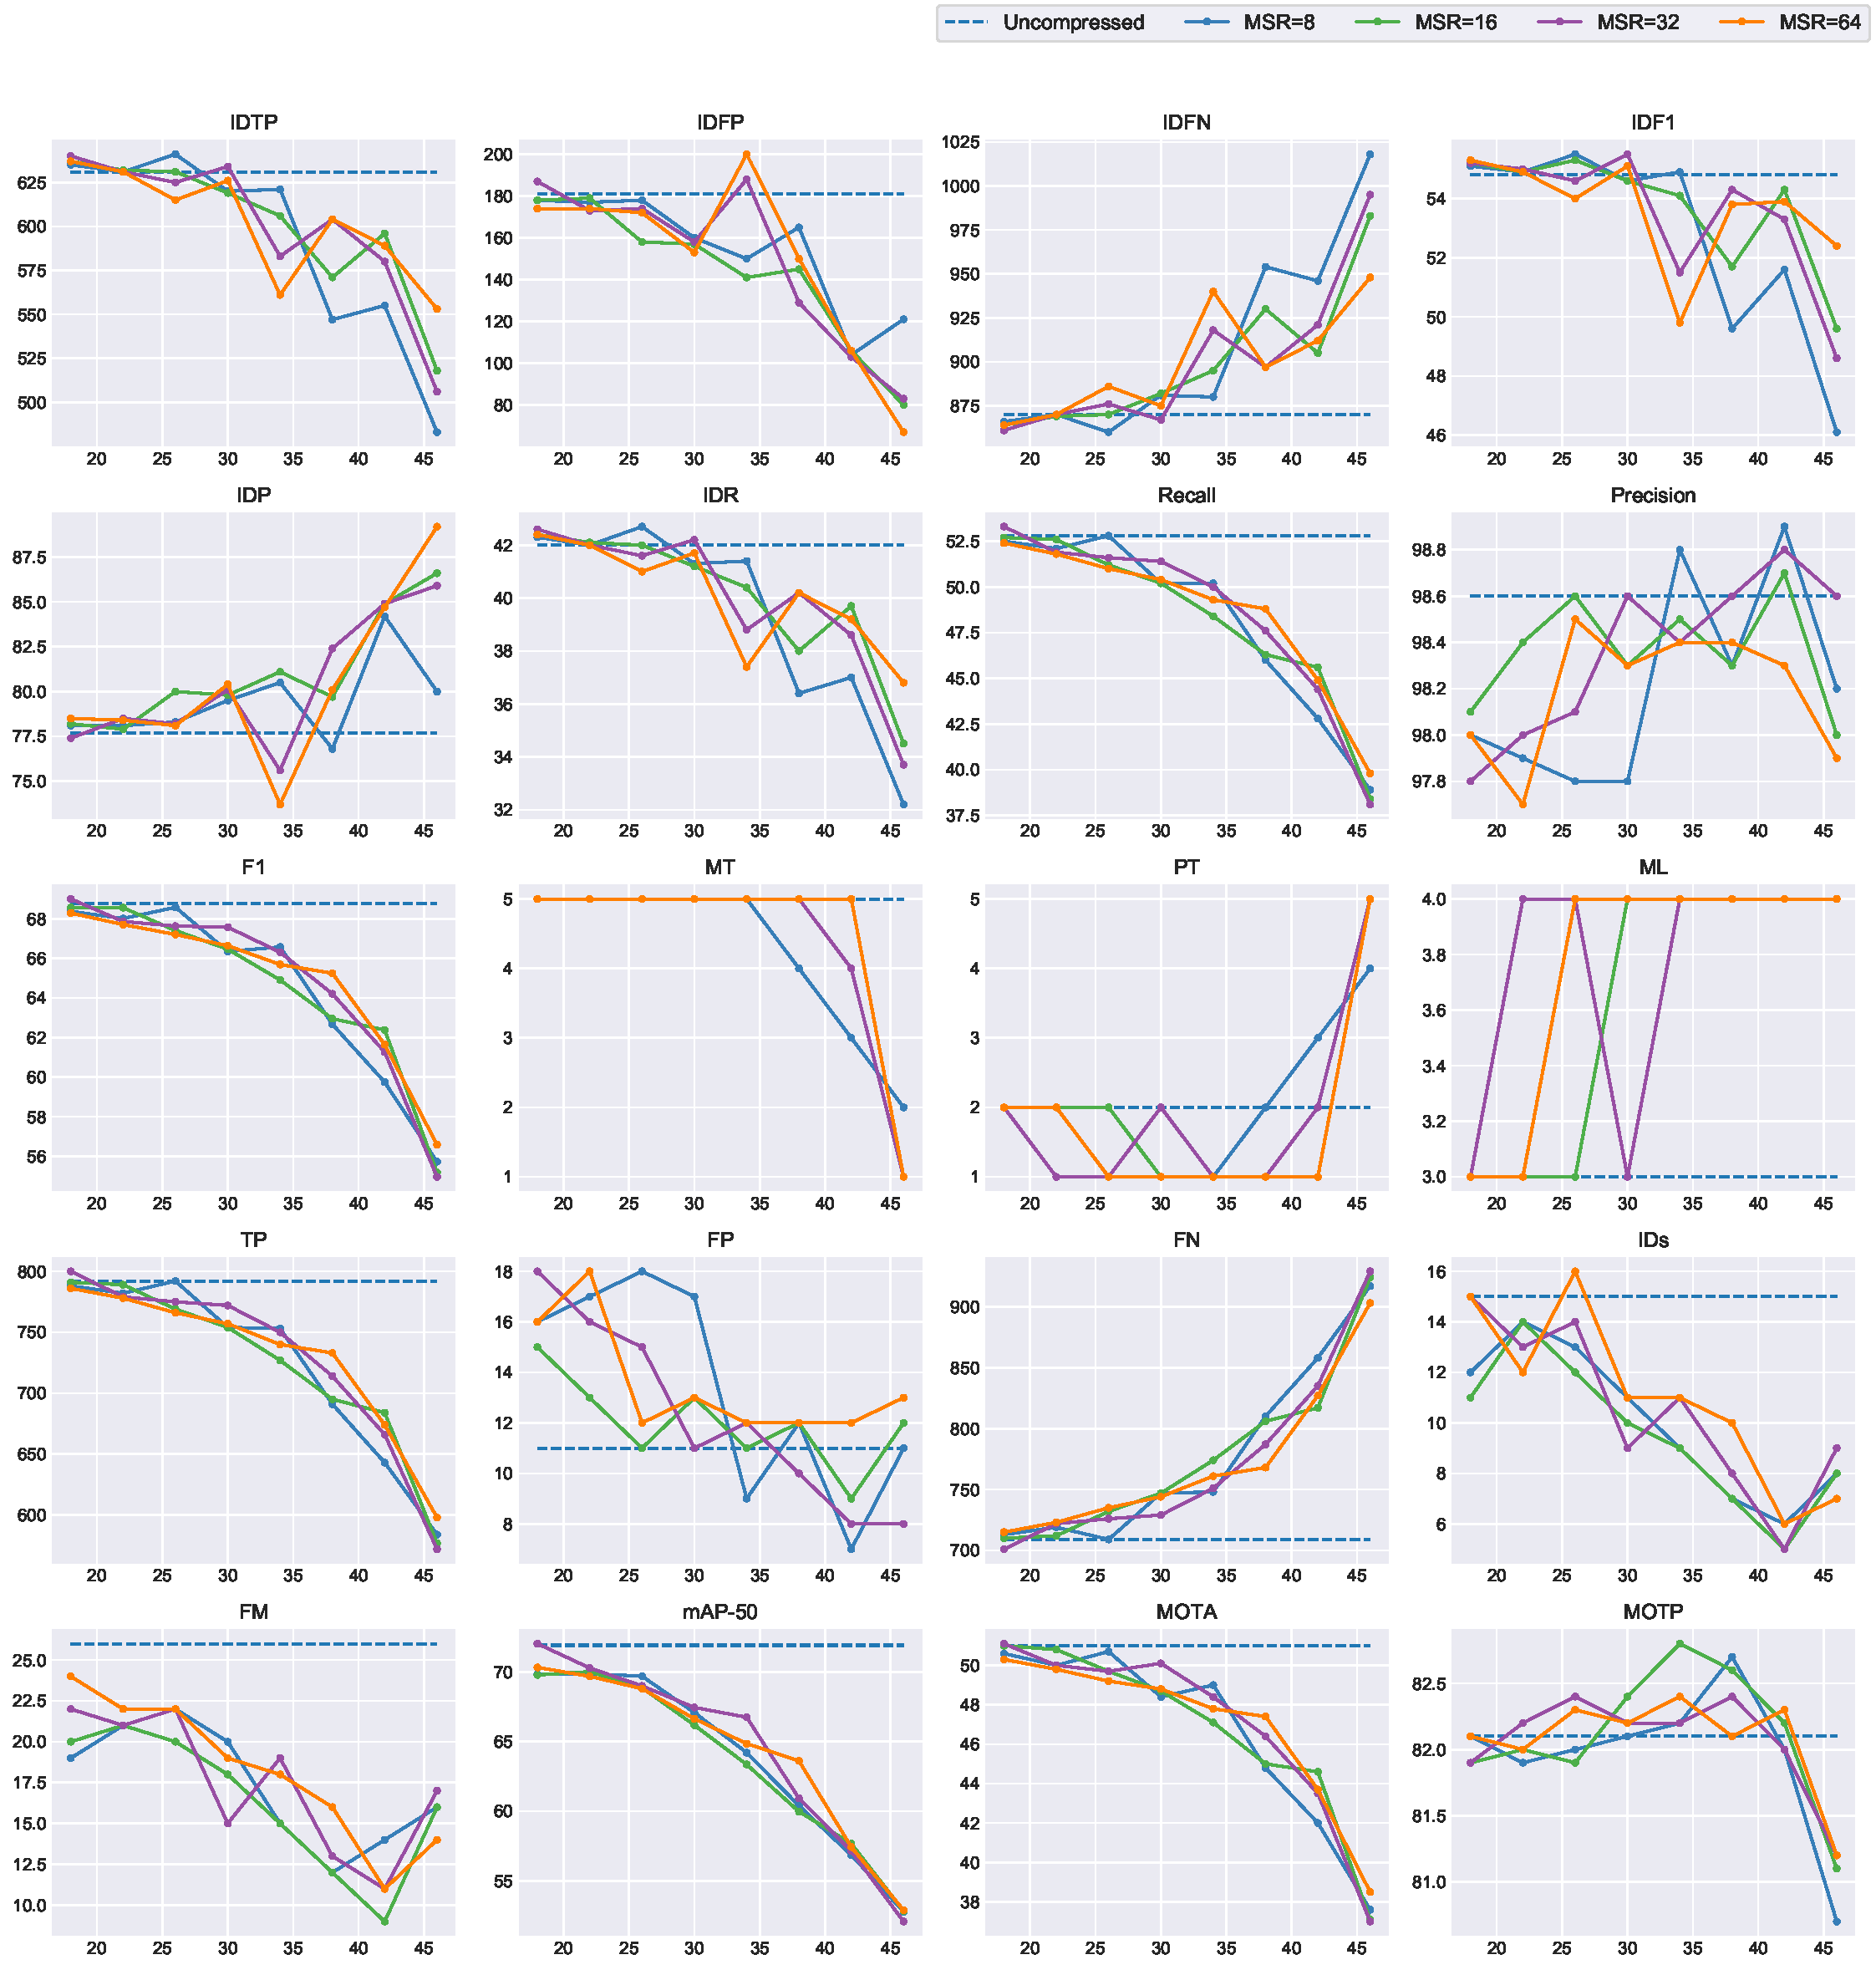
\includegraphics[width=1.0\linewidth]{img/appendix/ParkScene_all_multiplots_qp.pdf}
\caption[Result of all object classes in Class B ParkScene with Horizontal Axis of QP]{}
\label{fig:ParkScene_all_qp}
\end{figure}

\begin{figure}[!htbp]
\centering
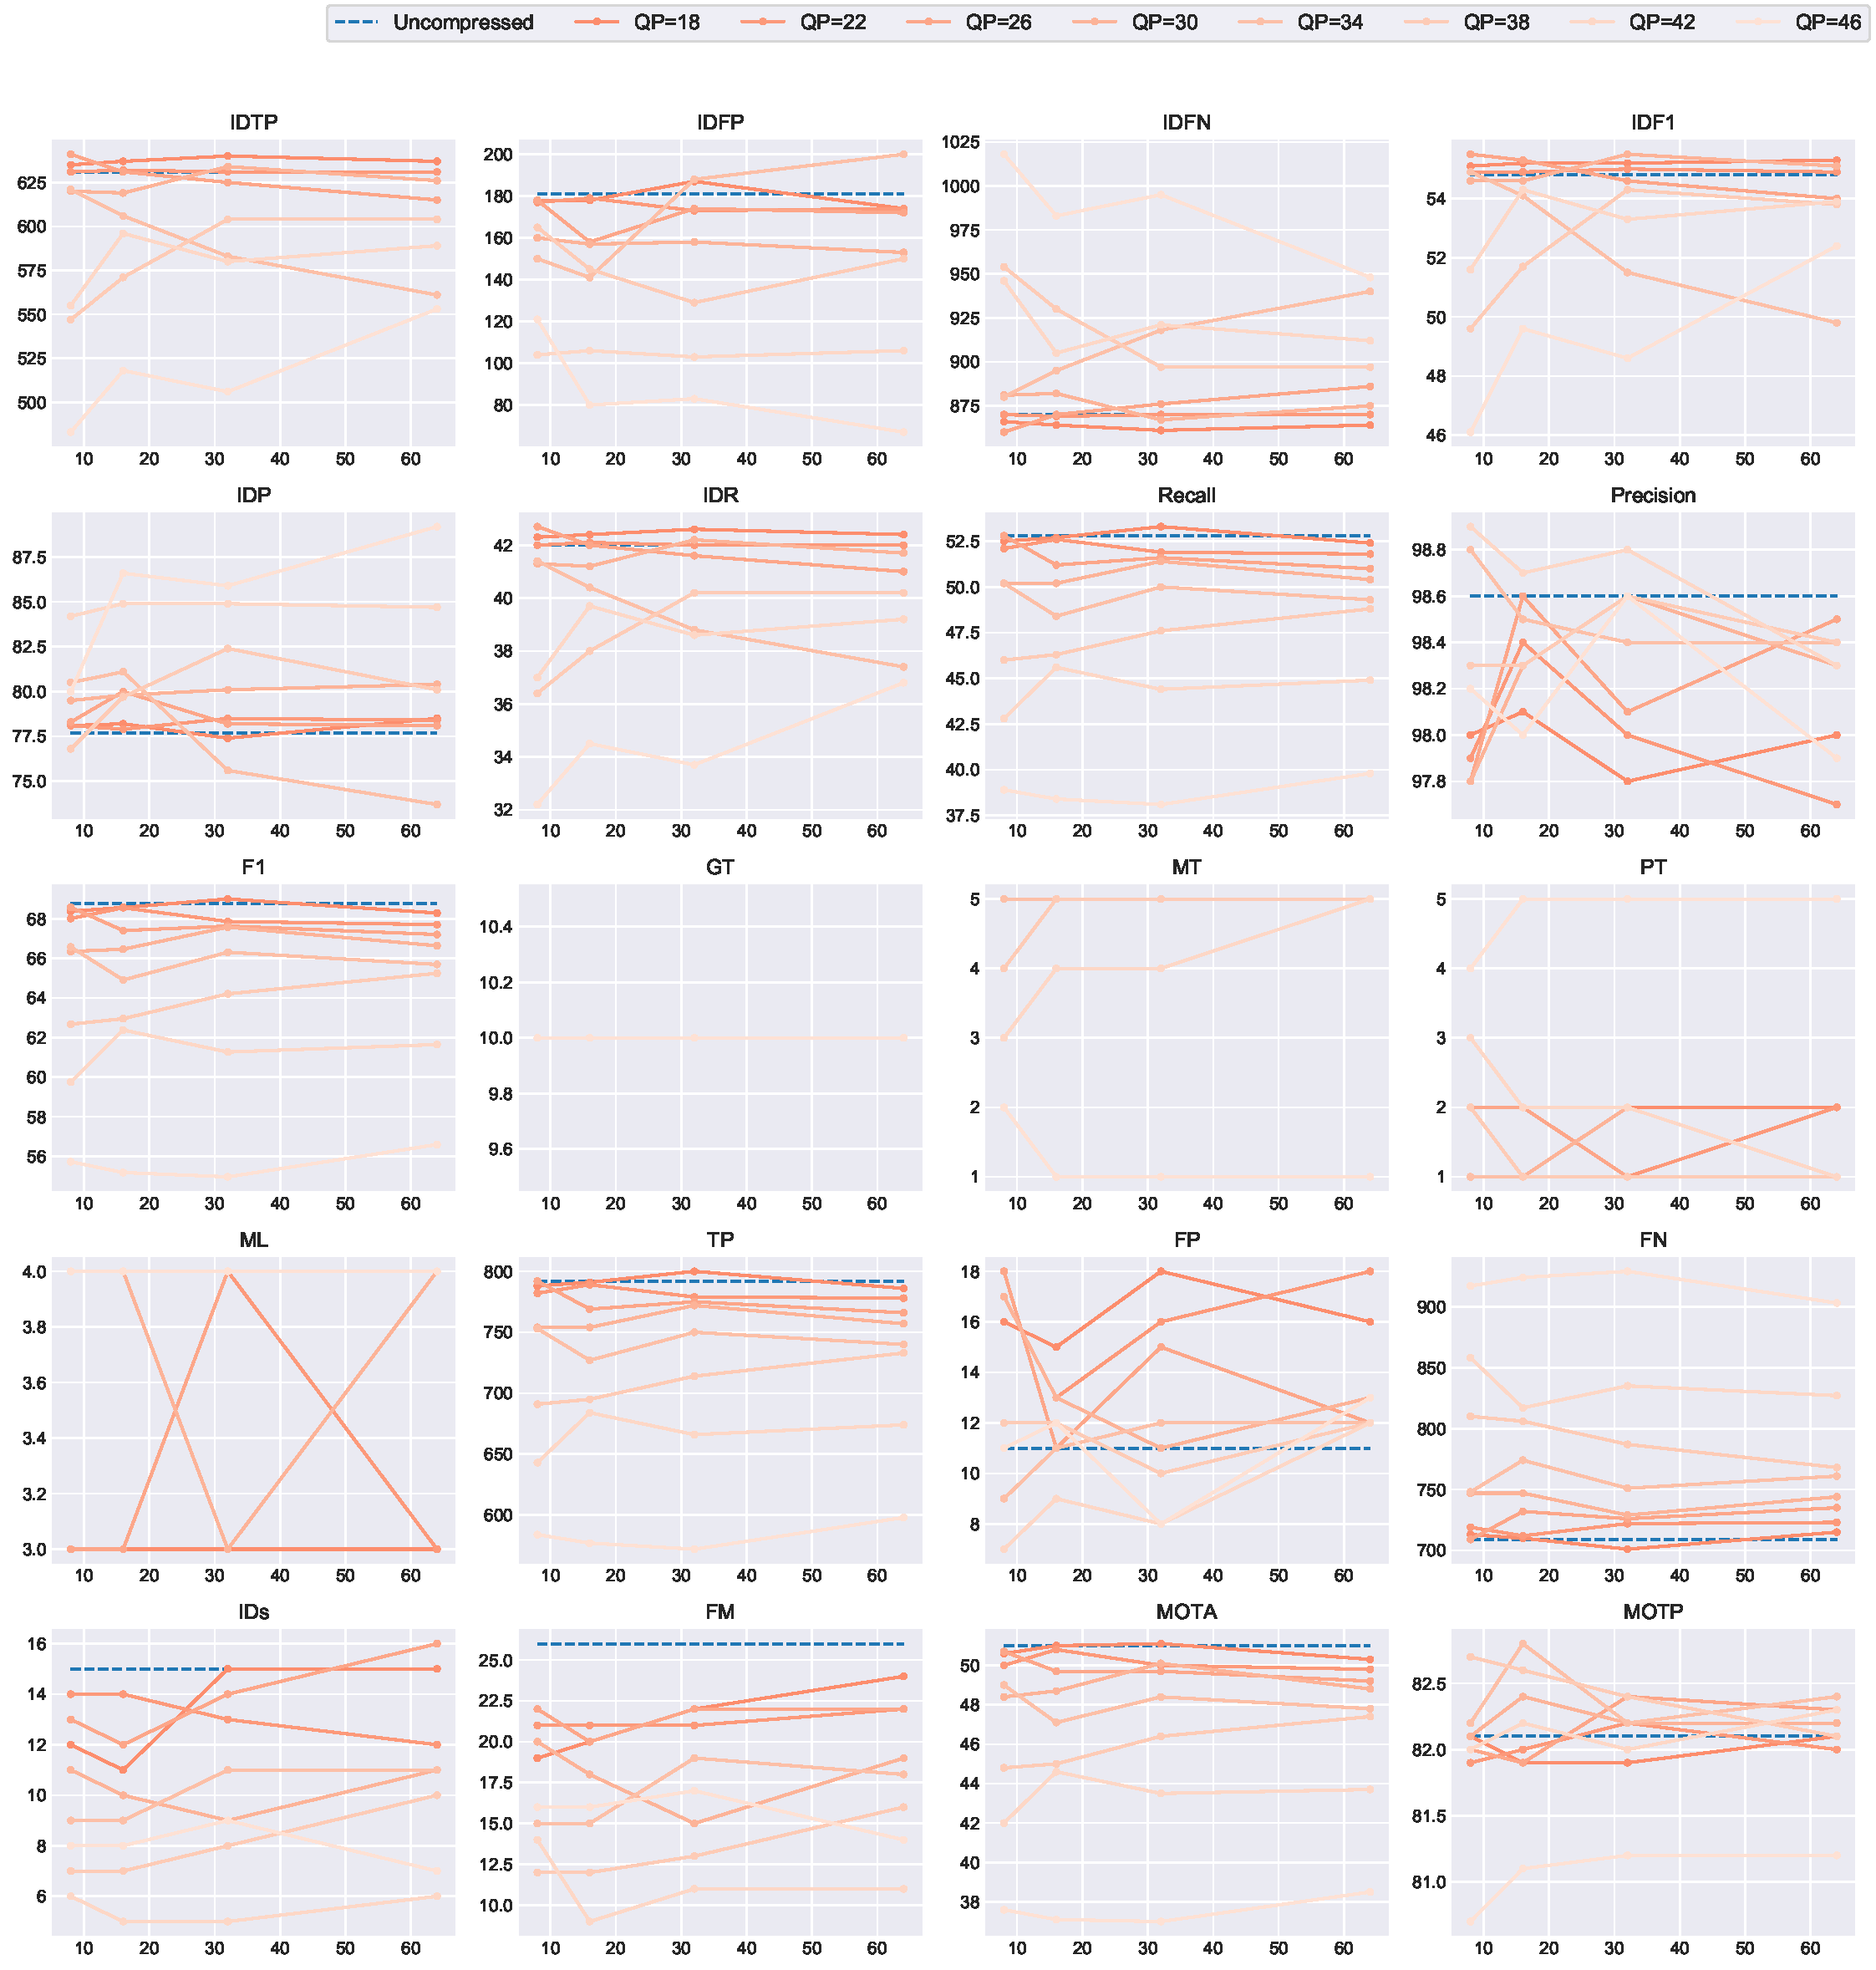
\includegraphics[width=1.0\linewidth]{img/appendix/ParkScene_all_multiplots_msr.pdf}
\caption[Result of all object classes in Class B ParkScene with Horizontal Axis of MSR]{}
\label{fig:ParkScene_all_msr}
\end{figure}



% table
\begin{table}
\centering
\caption{Result of all object classes in Class B ParkScene}


% table for uncompressed
\begin{subtable}[t]{\linewidth}
\centering
\vspace{0pt}
\resizebox{1.0\linewidth}{!}{
\begin{tabular}{llrrrrrrrrrrrrrrrrrrrr}
\toprule
          QP &          MSR &   IDTP &   IDFP &   IDFN &  IDF1 &   IDP &   IDR &  Recall &  Precision &    F1 &  GT &  MT &  PT &  ML &  TP &  FP &  FN &  IDs &  FM &  MOTA &  MOTP \\
\midrule
Uncompressed & Uncompressed & 631.00 & 181.00 & 870.00 & 54.80 & 77.70 & 42.00 &   52.80 &      98.60 & 68.77 &  10 &   5 &   2 &   3 & 792 &  11 & 709 &   15 &  26 & 51.00 & 82.10 \\
\bottomrule
\end{tabular}

}
\caption{Uncompressed Sequence}
\end{subtable}


% table for msr=8
\begin{subtable}[t]{\linewidth}
\centering
\resizebox{1.0\linewidth}{!}{
\begin{tabular}{rrrrrrrrrrrrrrrrrrrrrr}
\toprule
 QP &  MSR &   IDTP &   IDFP &    IDFN &  IDF1 &   IDP &   IDR &  Recall &  Precision &    F1 &  GT &  MT &  PT &  ML &  TP &  FP &  FN &  IDs &  FM &  MOTA &  MOTP \\
\midrule
 18 &    8 & 635.00 & 178.00 &  866.00 & 55.10 & 78.10 & 42.30 &   52.50 &      98.00 & 68.37 &  10 &   5 &   2 &   3 & 788 &  16 & 713 &   12 &  19 & 50.60 & 82.10 \\
 22 &    8 & 631.00 & 177.00 &  870.00 & 54.90 & 78.10 & 42.00 &   52.10 &      97.90 & 68.01 &  10 &   5 &   2 &   3 & 782 &  17 & 719 &   14 &  21 & 50.00 & 81.90 \\
 26 &    8 & 641.00 & 178.00 &  860.00 & 55.50 & 78.30 & 42.70 &   52.80 &      97.80 & 68.58 &  10 &   5 &   2 &   3 & 792 &  18 & 709 &   13 &  22 & 50.70 & 82.00 \\
 30 &    8 & 620.00 & 160.00 &  881.00 & 54.60 & 79.50 & 41.30 &   50.20 &      97.80 & 66.35 &  10 &   5 &   1 &   4 & 754 &  17 & 747 &   11 &  20 & 48.40 & 82.10 \\
 34 &    8 & 621.00 & 150.00 &  880.00 & 54.90 & 80.50 & 41.40 &   50.20 &      98.80 & 66.57 &  10 &   5 &   1 &   4 & 753 &   9 & 748 &    9 &  15 & 49.00 & 82.20 \\
 38 &    8 & 547.00 & 165.00 &  954.00 & 49.60 & 76.80 & 36.40 &   46.00 &      98.30 & 62.67 &  10 &   4 &   2 &   4 & 691 &  12 & 810 &    7 &  12 & 44.80 & 82.70 \\
 42 &    8 & 555.00 & 104.00 &  946.00 & 51.60 & 84.20 & 37.00 &   42.80 &      98.90 & 59.74 &  10 &   3 &   3 &   4 & 643 &   7 & 858 &    6 &  14 & 42.00 & 82.00 \\
 46 &    8 & 483.00 & 121.00 & 1018.00 & 46.10 & 80.00 & 32.20 &   38.90 &      98.20 & 55.73 &  10 &   2 &   4 &   4 & 584 &  11 & 917 &    8 &  16 & 37.60 & 80.70 \\
\bottomrule
\end{tabular}

}
\caption{MSR = 8}
\end{subtable}



% table for msr=16
\begin{subtable}[t]{\linewidth}
\centering
\resizebox{1.0\linewidth}{!}{
\begin{tabular}{rrrrrrrrrrrrrrrrrrrrrr}
\toprule
 QP &  MSR &   IDTP &   IDFP &   IDFN &  IDF1 &   IDP &   IDR &  Recall &  Precision &    F1 &  GT &  MT &  PT &  ML &  TP &  FP &  FN &  IDs &  FM &  MOTA &  MOTP \\
\midrule
 18 &   16 & 637.00 & 178.00 & 864.00 & 55.20 & 78.20 & 42.40 &   52.70 &      98.10 & 68.57 &  10 &   5 &   2 &   3 & 791 &  15 & 710 &   11 &  20 & 51.00 & 81.90 \\
 22 &   16 & 632.00 & 179.00 & 869.00 & 54.90 & 77.90 & 42.10 &   52.60 &      98.40 & 68.55 &  10 &   5 &   2 &   3 & 789 &  13 & 712 &   14 &  21 & 50.80 & 82.00 \\
 26 &   16 & 631.00 & 158.00 & 870.00 & 55.30 & 80.00 & 42.00 &   51.20 &      98.60 & 67.40 &  10 &   5 &   2 &   3 & 769 &  11 & 732 &   12 &  20 & 49.70 & 81.90 \\
 30 &   16 & 619.00 & 157.00 & 882.00 & 54.60 & 79.80 & 41.20 &   50.20 &      98.30 & 66.46 &  10 &   5 &   1 &   4 & 754 &  13 & 747 &   10 &  18 & 48.70 & 82.40 \\
 34 &   16 & 606.00 & 141.00 & 895.00 & 54.10 & 81.10 & 40.40 &   48.40 &      98.50 & 64.91 &  10 &   5 &   1 &   4 & 727 &  11 & 774 &    9 &  15 & 47.10 & 82.80 \\
 38 &   16 & 571.00 & 145.00 & 930.00 & 51.70 & 79.70 & 38.00 &   46.30 &      98.30 & 62.95 &  10 &   5 &   1 &   4 & 695 &  12 & 806 &    7 &  12 & 45.00 & 82.60 \\
 42 &   16 & 596.00 & 106.00 & 905.00 & 54.30 & 84.90 & 39.70 &   45.60 &      98.70 & 62.38 &  10 &   4 &   2 &   4 & 684 &   9 & 817 &    5 &   9 & 44.60 & 82.20 \\
 46 &   16 & 518.00 &  80.00 & 983.00 & 49.60 & 86.60 & 34.50 &   38.40 &      98.00 & 55.18 &  10 &   1 &   5 &   4 & 577 &  12 & 924 &    8 &  16 & 37.10 & 81.10 \\
\bottomrule
\end{tabular}

}
\caption{MSR = 16}
\end{subtable}


% table for msr=32
\begin{subtable}[t]{\linewidth}
\centering
\resizebox{1.0\linewidth}{!}{
\begin{tabular}{rrrrrrrrrrrrrrrrrrrrrr}
\toprule
 QP &  MSR &   IDTP &   IDFP &   IDFN &  IDF1 &   IDP &   IDR &  Recall &  Precision &    F1 &  GT &  MT &  PT &  ML &  TP &  FP &  FN &  IDs &  FM &  MOTA &  MOTP \\
\midrule
 18 &   32 & 640.00 & 187.00 & 861.00 & 55.20 & 77.40 & 42.60 &   53.30 &      97.80 & 69.00 &  10 &   5 &   2 &   3 & 800 &  18 & 701 &   15 &  22 & 51.10 & 81.90 \\
 22 &   32 & 631.00 & 173.00 & 870.00 & 55.00 & 78.50 & 42.00 &   51.90 &      98.00 & 67.86 &  10 &   5 &   1 &   4 & 779 &  16 & 722 &   13 &  21 & 50.00 & 82.20 \\
 26 &   32 & 625.00 & 174.00 & 876.00 & 54.60 & 78.20 & 41.60 &   51.60 &      98.10 & 67.63 &  10 &   5 &   1 &   4 & 775 &  15 & 726 &   14 &  22 & 49.70 & 82.40 \\
 30 &   32 & 634.00 & 158.00 & 867.00 & 55.50 & 80.10 & 42.20 &   51.40 &      98.60 & 67.57 &  10 &   5 &   2 &   3 & 772 &  11 & 729 &    9 &  15 & 50.10 & 82.20 \\
 34 &   32 & 583.00 & 188.00 & 918.00 & 51.50 & 75.60 & 38.80 &   50.00 &      98.40 & 66.31 &  10 &   5 &   1 &   4 & 750 &  12 & 751 &   11 &  19 & 48.40 & 82.20 \\
 38 &   32 & 604.00 & 129.00 & 897.00 & 54.30 & 82.40 & 40.20 &   47.60 &      98.60 & 64.20 &  10 &   5 &   1 &   4 & 714 &  10 & 787 &    8 &  13 & 46.40 & 82.40 \\
 42 &   32 & 580.00 & 103.00 & 921.00 & 53.30 & 84.90 & 38.60 &   44.40 &      98.80 & 61.27 &  10 &   4 &   2 &   4 & 666 &   8 & 835 &    5 &  11 & 43.50 & 82.00 \\
 46 &   32 & 506.00 &  83.00 & 995.00 & 48.60 & 85.90 & 33.70 &   38.10 &      98.60 & 54.96 &  10 &   1 &   5 &   4 & 572 &   8 & 929 &    9 &  17 & 37.00 & 81.20 \\
\bottomrule
\end{tabular}

}
\caption{MSR = 32}
\end{subtable}


% table for msr=64
\begin{subtable}[t]{\linewidth}
\centering
\resizebox{1.0\linewidth}{!}{
\begin{tabular}{rrrrrrrrrrrrrrrrrrrrrr}
\toprule
 QP &  MSR &   IDTP &   IDFP &   IDFN &  IDF1 &   IDP &   IDR &  Recall &  Precision &    F1 &  GT &  MT &  PT &  ML &  TP &  FP &  FN &  IDs &  FM &  MOTA &  MOTP \\
\midrule
 18 &   64 & 637.00 & 174.00 & 864.00 & 55.30 & 78.50 & 42.40 &   52.40 &      98.00 & 68.29 &  10 &   5 &   2 &   3 & 786 &  16 & 715 &   15 &  24 & 50.30 & 82.10 \\
 22 &   64 & 631.00 & 174.00 & 870.00 & 54.90 & 78.40 & 42.00 &   51.80 &      97.70 & 67.70 &  10 &   5 &   2 &   3 & 778 &  18 & 723 &   12 &  22 & 49.80 & 82.00 \\
 26 &   64 & 615.00 & 172.00 & 886.00 & 54.00 & 78.10 & 41.00 &   51.00 &      98.50 & 67.20 &  10 &   5 &   1 &   4 & 766 &  12 & 735 &   16 &  22 & 49.20 & 82.30 \\
 30 &   64 & 626.00 & 153.00 & 875.00 & 55.10 & 80.40 & 41.70 &   50.40 &      98.30 & 66.64 &  10 &   5 &   1 &   4 & 757 &  13 & 744 &   11 &  19 & 48.80 & 82.20 \\
 34 &   64 & 561.00 & 200.00 & 940.00 & 49.80 & 73.70 & 37.40 &   49.30 &      98.40 & 65.69 &  10 &   5 &   1 &   4 & 740 &  12 & 761 &   11 &  18 & 47.80 & 82.40 \\
 38 &   64 & 604.00 & 150.00 & 897.00 & 53.80 & 80.10 & 40.20 &   48.80 &      98.40 & 65.24 &  10 &   5 &   1 &   4 & 733 &  12 & 768 &   10 &  16 & 47.40 & 82.10 \\
 42 &   64 & 589.00 & 106.00 & 912.00 & 53.90 & 84.70 & 39.20 &   44.90 &      98.30 & 61.64 &  10 &   5 &   1 &   4 & 674 &  12 & 827 &    6 &  11 & 43.70 & 82.30 \\
 46 &   64 & 553.00 &  67.00 & 948.00 & 52.40 & 89.20 & 36.80 &   39.80 &      97.90 & 56.59 &  10 &   1 &   5 &   4 & 598 &  13 & 903 &    7 &  14 & 38.50 & 81.20 \\
\bottomrule
\end{tabular}

}
\caption{MSR = 64}
\end{subtable}


\label{tab:ParkScene_all}
\end{table}




\begin{table}[!htbp]
\centering
\caption{Multiple Linear Regression Analysis Result for Class B ParkScene}
\resizebox{1.0\linewidth}{!}{
\begin{tabular}{lrrrrrrrrrrrrrrrrrrr}
\toprule
{} &   IDTP &   IDFP &   IDFN &  IDF1 &   IDP &   IDR &  Recall &  Precision &    F1 &    MT &    PT &    ML &     TP &    FP &     FN &   IDs &    FM &  MOTA &  MOTP \\
\midrule
coefficient(Intercept) & 750.99 & 239.06 & 750.01 & 61.51 & 74.49 & 49.97 &   63.93 &      97.64 & 78.89 &  7.61 &  0.15 &  2.24 & 959.31 & 21.75 & 541.69 & 17.42 & 25.23 & 61.32 & 82.50 \\
coefficient(QP)        &  -4.88 &  -2.81 &   4.88 & -0.26 &  0.18 & -0.32 &   -0.49 &       0.02 & -0.45 & -0.10 &  0.06 &  0.04 &  -7.39 & -0.29 &   7.39 & -0.25 & -0.27 & -0.46 & -0.01 \\
coefficient(MSR)       &  -1.00 &   0.34 &   1.00 & -0.08 & -0.08 & -0.07 &   -0.04 &       0.00 & -0.04 & -0.01 & -0.00 &  0.01 &  -0.62 & -0.04 &   0.62 &  0.06 &  0.10 & -0.04 &  0.00 \\
coefficient(QP*MSR)    &   0.04 &  -0.01 &  -0.04 &  0.00 &  0.00 &  0.00 &    0.00 &      -0.00 &  0.00 &  0.00 & -0.00 & -0.00 &   0.02 &  0.00 &  -0.02 & -0.00 & -0.00 &  0.00 & -0.00 \\
p-value(Intercept)     &   0.00 &   0.00 &   0.00 &  0.00 &  0.00 &  0.00 &    0.00 &       0.00 &  0.00 &  0.00 &  0.91 &  0.00 &   0.00 &  0.00 &   0.00 &  0.00 &  0.00 &  0.00 &  0.00 \\
p-value(QP)            &   0.00 &   0.00 &   0.00 &  0.00 &  0.05 &  0.00 &    0.00 &       0.04 &  0.00 &  0.00 &  0.11 &  0.00 &   0.00 &  0.00 &   0.00 &  0.00 &  0.00 &  0.00 &  0.33 \\
p-value(MSR)           &   0.15 &   0.59 &   0.15 &  0.13 &  0.33 &  0.16 &    0.49 &       0.67 &  0.52 &  0.84 &  0.95 &  0.40 &   0.49 &  0.54 &   0.49 &  0.27 &  0.17 &  0.49 &  0.93 \\
p-value(QP*MSR)        &   0.10 &   0.56 &   0.10 &  0.08 &  0.27 &  0.10 &    0.40 &       0.54 &  0.43 &  0.73 &  0.91 &  0.53 &   0.39 &  0.41 &   0.39 &  0.49 &  0.28 &  0.42 &  0.99 \\
\bottomrule
\end{tabular}

}
\label{tab:ParkScene_all_reg}
\end{table}



\newpage

\section{Class C BasketballDrill}
\label{sec:appendix/BasketballDrill_all}


% visualization figure
\begin{figure}[!htbp]
\centering
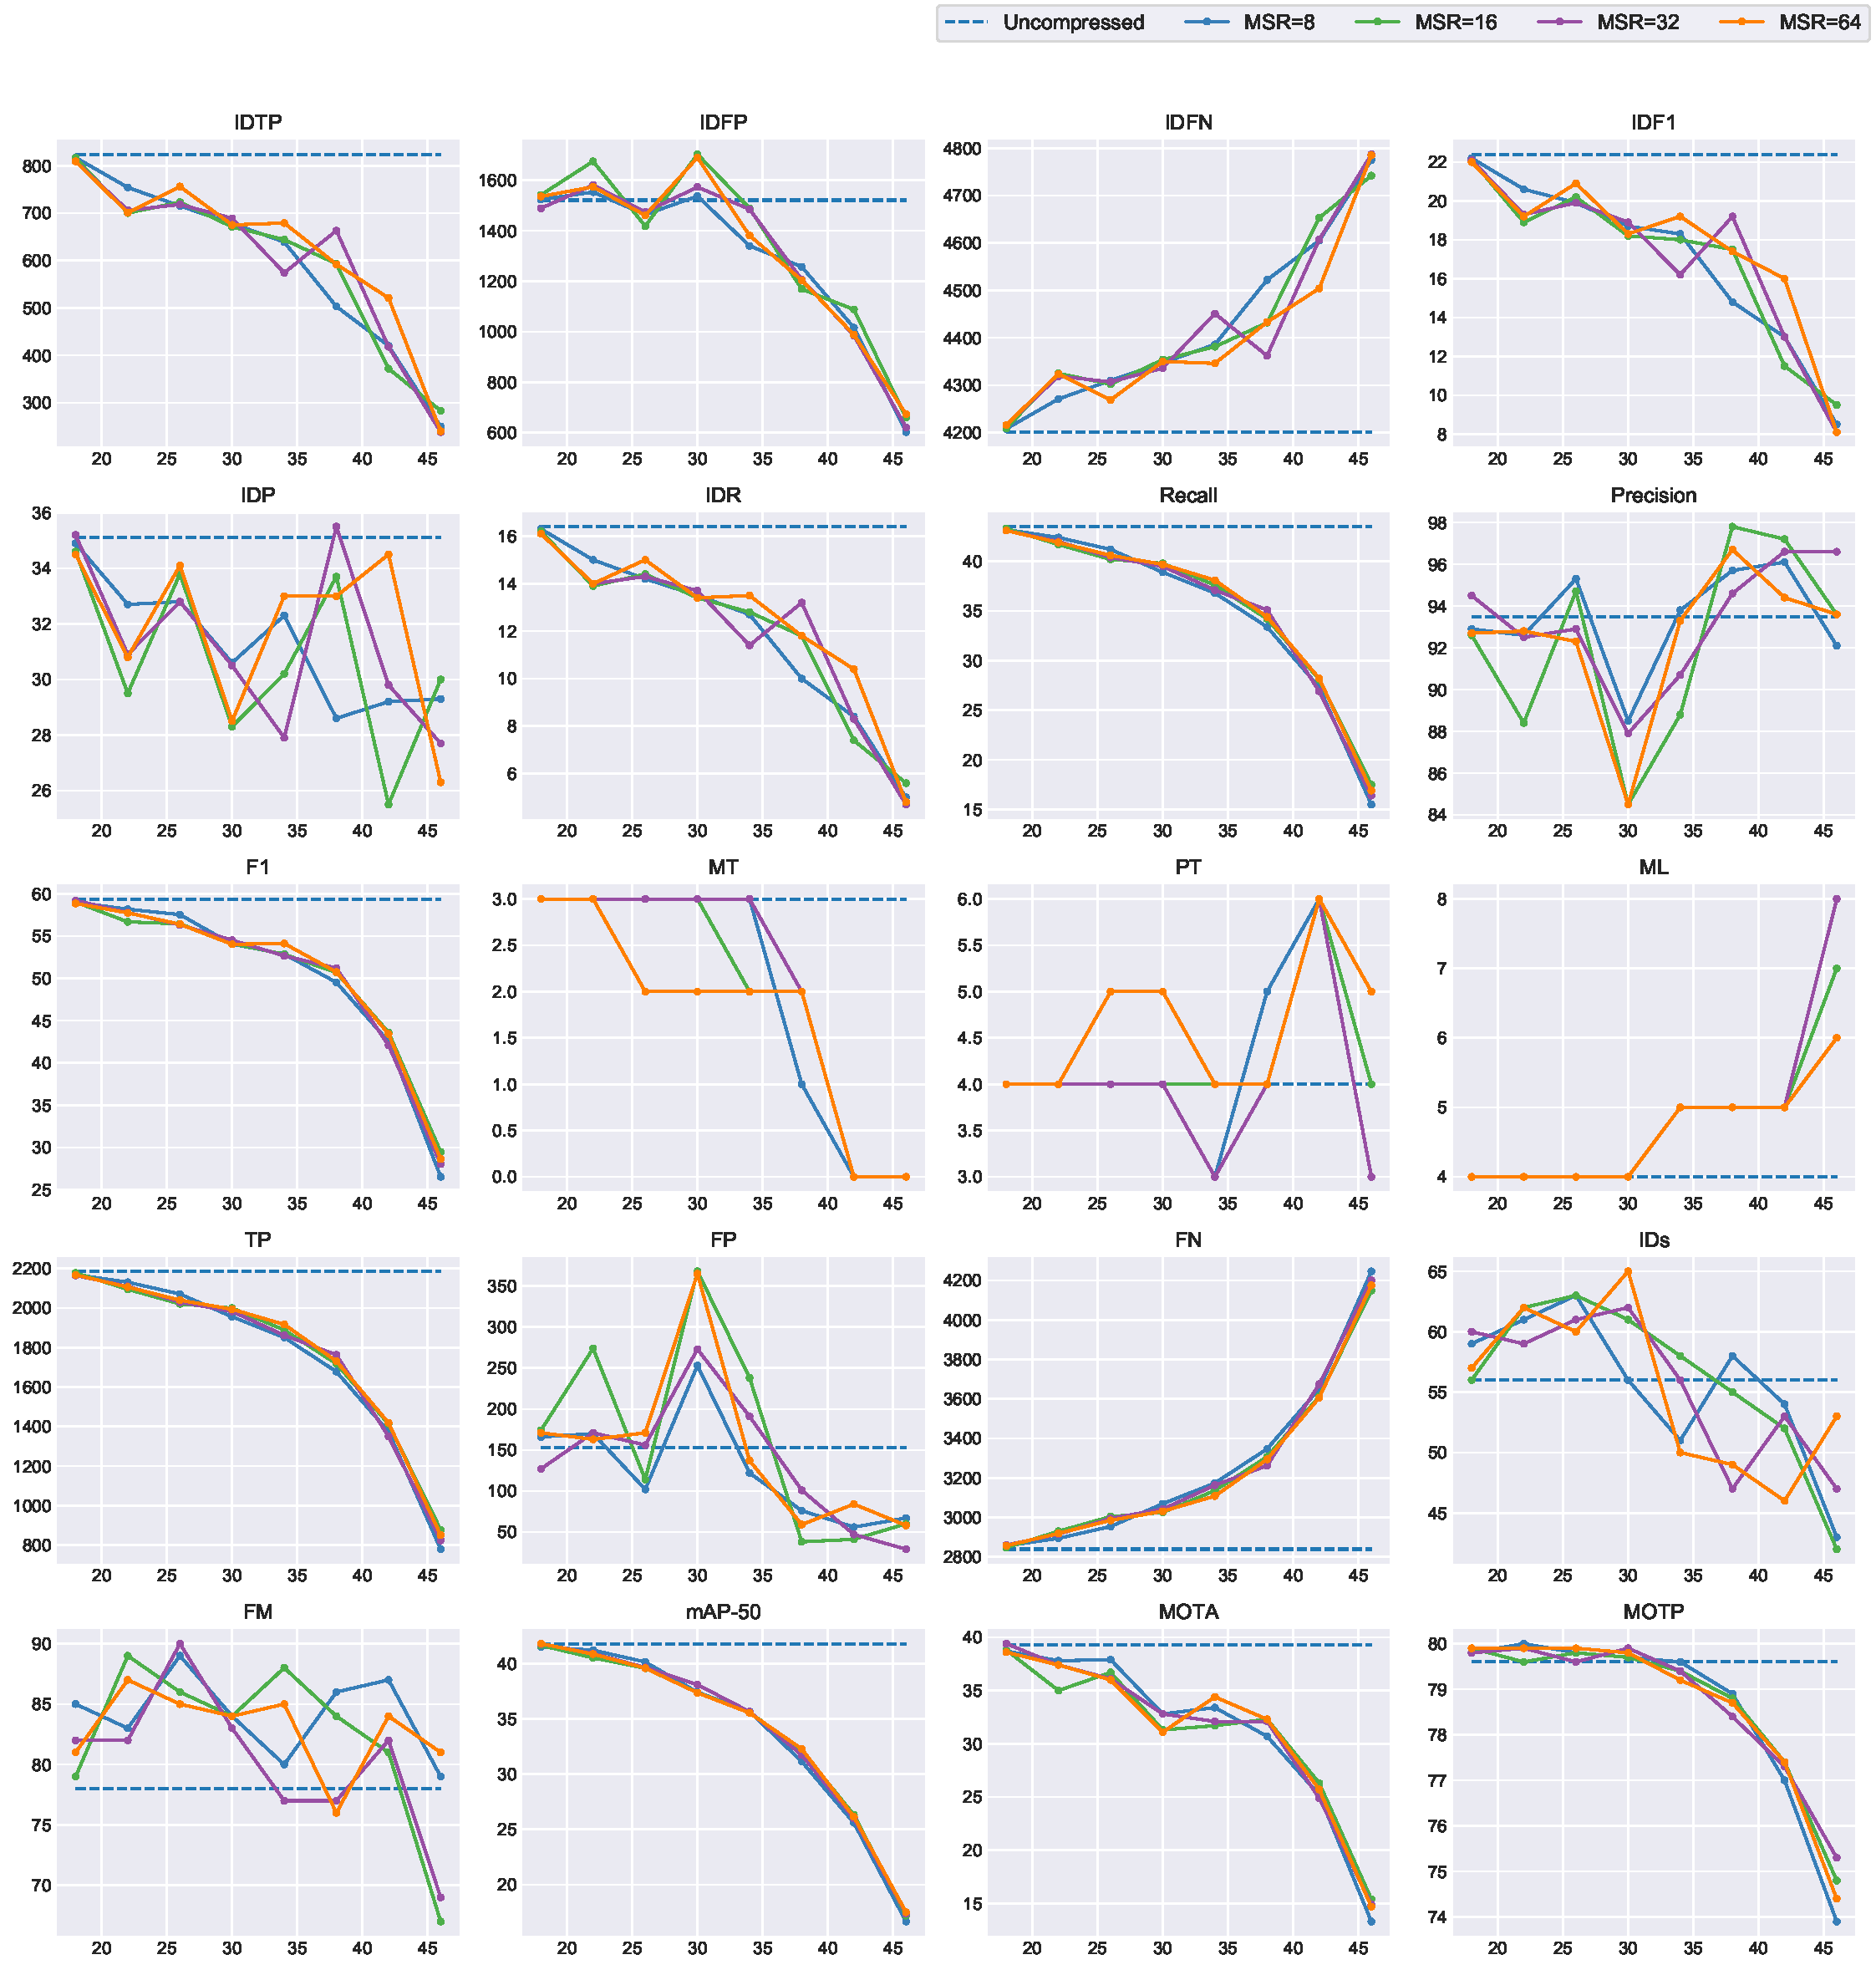
\includegraphics[width=1.0\linewidth]{img/appendix/BasketballDrill_all_multiplots_qp.pdf}
\caption[Result of all object classes in Class C BasketballDrill with Horizontal Axis of QP]{}
\label{fig:BasketballDrill_all_qp}
\end{figure}

\begin{figure}[!htbp]
\centering
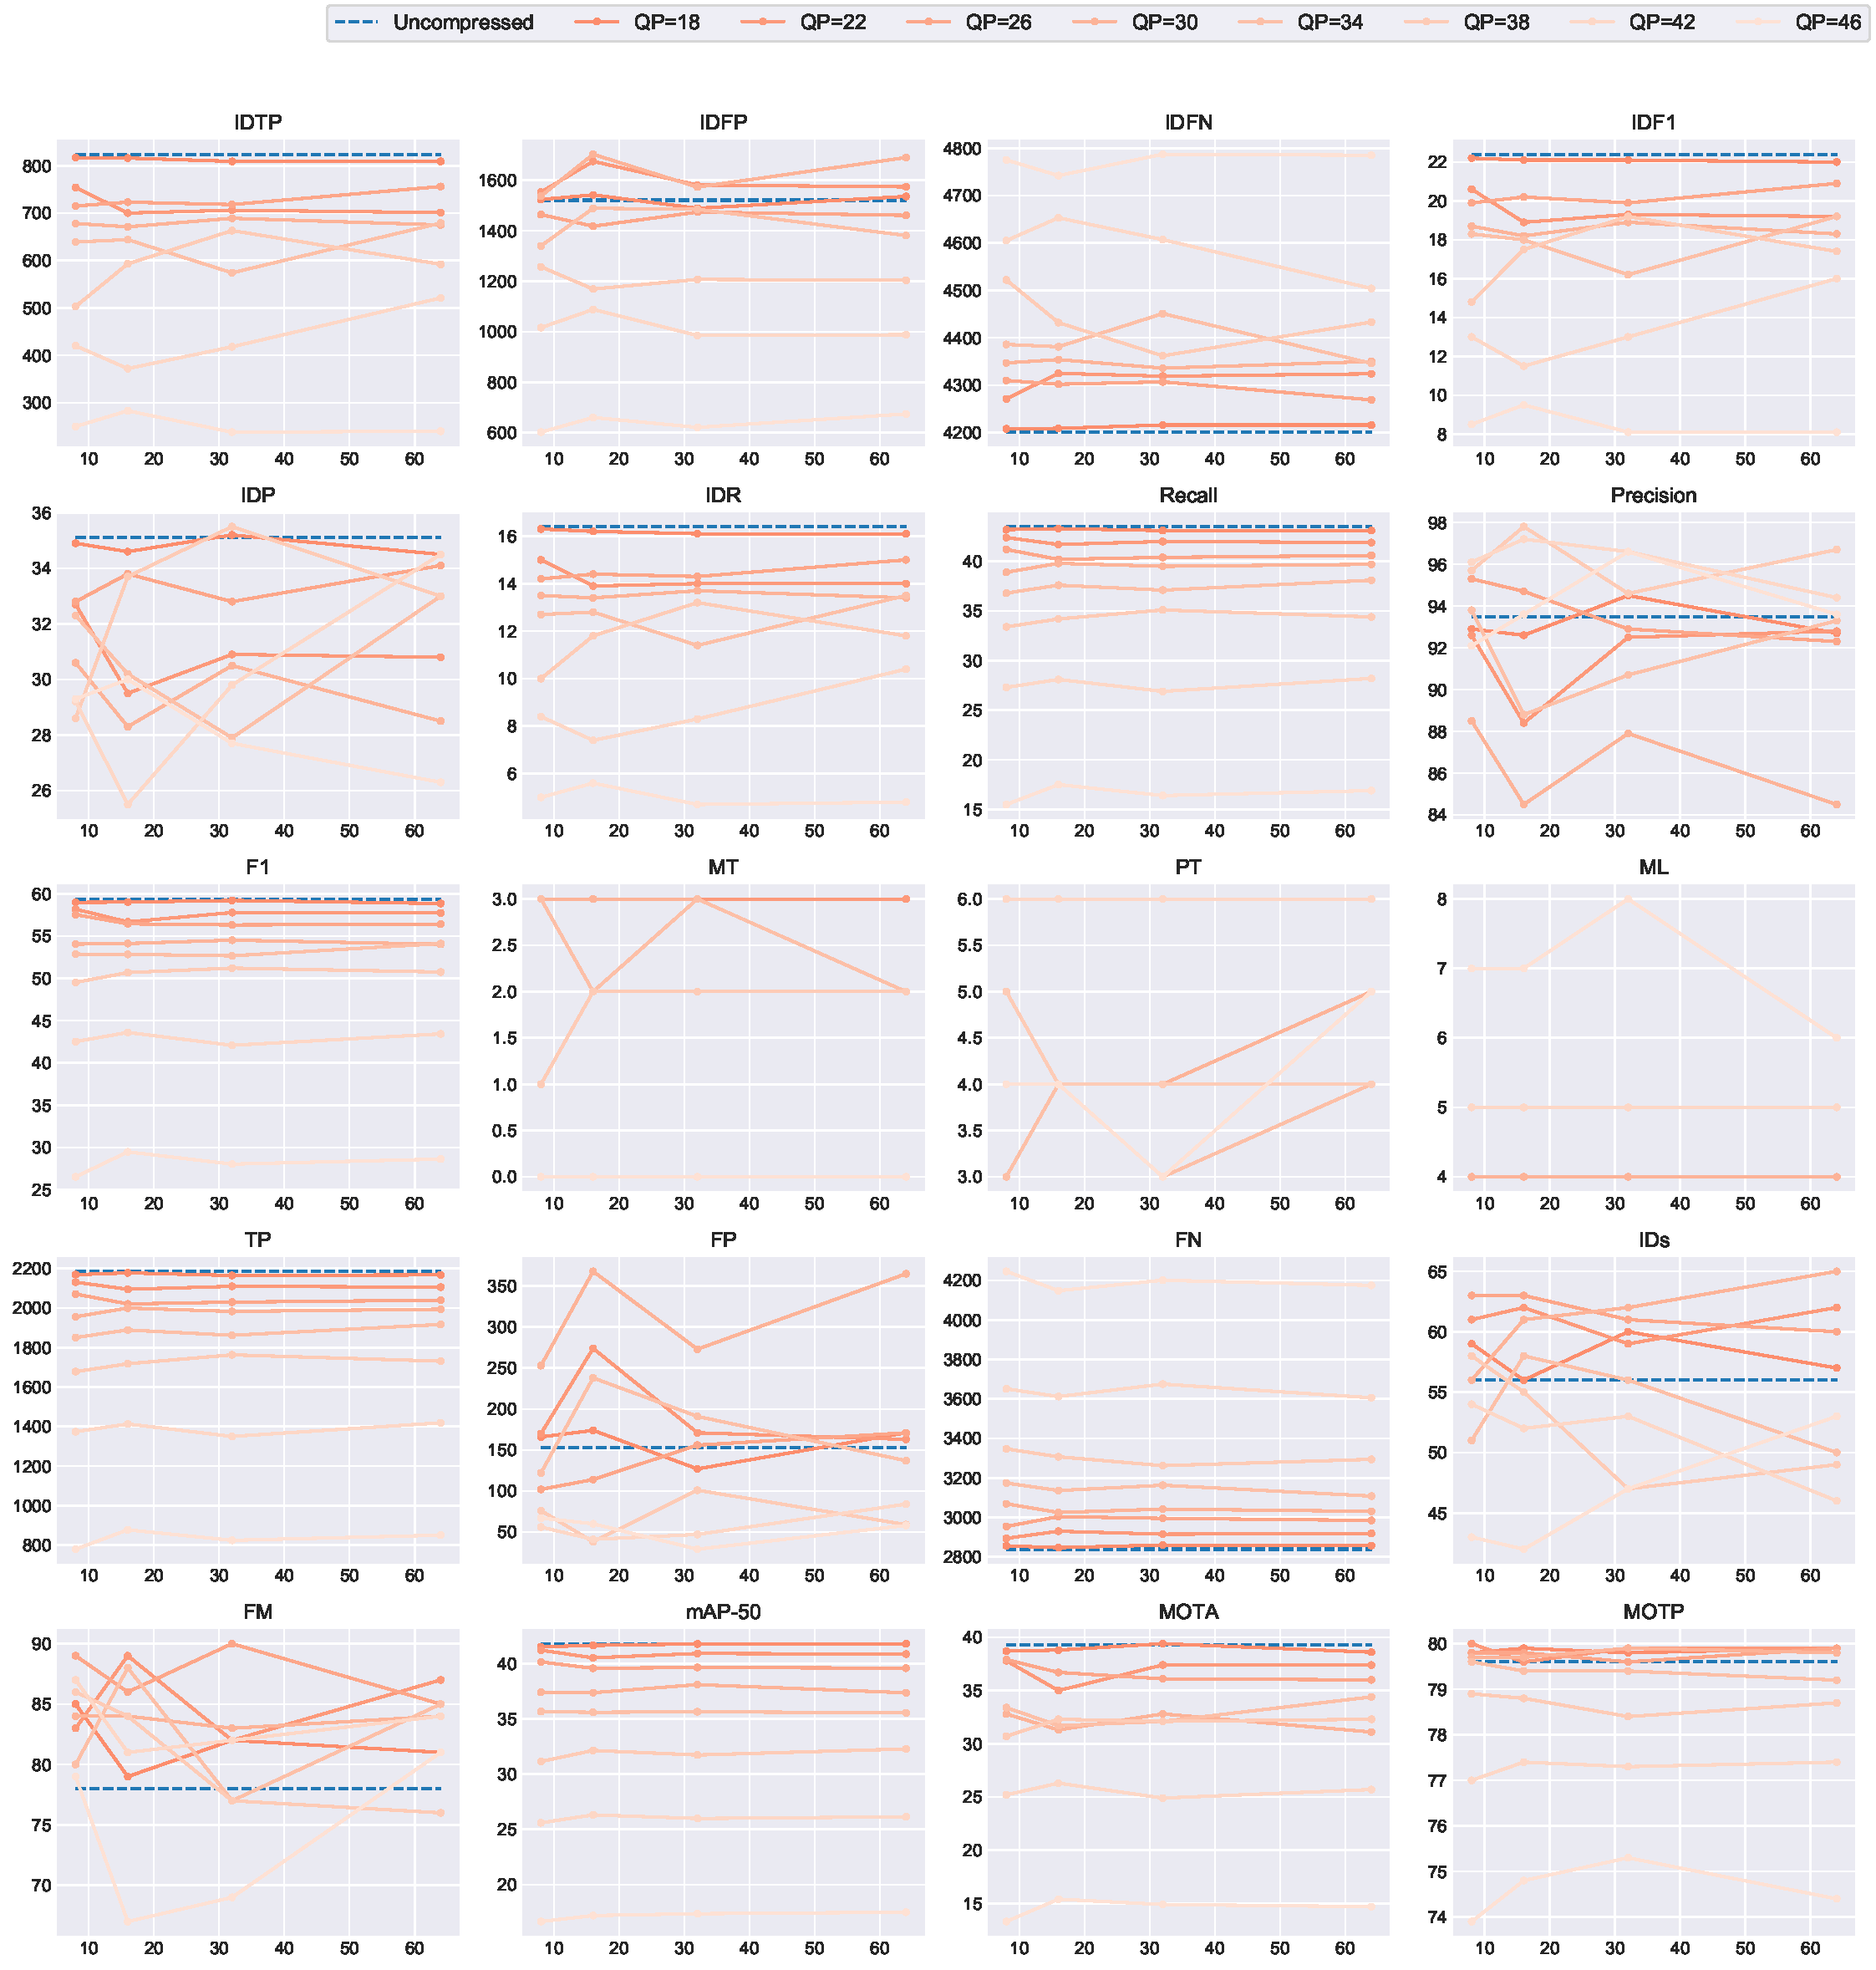
\includegraphics[width=1.0\linewidth]{img/appendix/BasketballDrill_all_multiplots_msr.pdf}
\caption[Result of all object classes in Class C BasketballDrill with Horizontal Axis of MSR]{}
\label{fig:BasketballDrill_all_msr}
\end{figure}



% table
\begin{table}
\centering
\caption{Result of all object classes in Class C BasketballDrill}


% table for uncompressed
\begin{subtable}[t]{\linewidth}
\centering
\vspace{0pt}
\resizebox{1.0\linewidth}{!}{
\begin{tabular}{llrrrrrrrrrrrrrrrrrrrr}
\toprule
          QP &          MSR &   IDTP &    IDFP &    IDFN &  IDF1 &   IDP &   IDR &  Recall &  Precision &    F1 &  GT &  MT &  PT &  ML &   TP &  FP &   FN &  IDs &  FM &  MOTA &  MOTP \\
\midrule
Uncompressed & Uncompressed & 824.00 & 1521.00 & 4201.00 & 22.40 & 35.10 & 16.40 &   43.50 &      93.50 & 59.38 &  11 &   3 &   4 &   4 & 2186 & 153 & 2839 &   56 &  78 & 39.30 & 79.60 \\
\bottomrule
\end{tabular}

}
\caption{Uncompressed Sequence}
\end{subtable}


% table for msr=8
\begin{subtable}[t]{\linewidth}
\centering
\resizebox{1.0\linewidth}{!}{
\begin{tabular}{rrrrrrrrrrrrrrrrrrrrrr}
\toprule
 QP &  MSR &   IDTP &    IDFP &    IDFN &  IDF1 &   IDP &   IDR &  Recall &  Precision &    F1 &  GT &  MT &  PT &  ML &   TP &  FP &   FN &  IDs &  FM &  MOTA &  MOTP \\
\midrule
 18 &    8 & 817.00 & 1524.00 & 4208.00 & 22.20 & 34.90 & 16.30 &   43.20 &      92.90 & 58.98 &  11 &   3 &   4 &   4 & 2169 & 166 & 2856 &   59 &  85 & 38.70 & 79.80 \\
 22 &    8 & 754.00 & 1553.00 & 4271.00 & 20.60 & 32.70 & 15.00 &   42.40 &      92.60 & 58.17 &  11 &   3 &   4 &   4 & 2131 & 170 & 2894 &   61 &  83 & 37.80 & 80.00 \\
 26 &    8 & 715.00 & 1464.00 & 4310.00 & 19.90 & 32.80 & 14.20 &   41.20 &      95.30 & 57.53 &  11 &   3 &   4 &   4 & 2071 & 102 & 2954 &   63 &  89 & 37.90 & 79.80 \\
 30 &    8 & 678.00 & 1537.00 & 4347.00 & 18.70 & 30.60 & 13.50 &   38.90 &      88.50 & 54.04 &  11 &   3 &   4 &   4 & 1956 & 253 & 3069 &   56 &  84 & 32.80 & 79.70 \\
 34 &    8 & 639.00 & 1340.00 & 4386.00 & 18.30 & 32.30 & 12.70 &   36.80 &      93.80 & 52.86 &  11 &   3 &   3 &   5 & 1851 & 122 & 3174 &   51 &  80 & 33.40 & 79.60 \\
 38 &    8 & 503.00 & 1257.00 & 4522.00 & 14.80 & 28.60 & 10.00 &   33.40 &      95.70 & 49.52 &  11 &   1 &   5 &   5 & 1678 &  76 & 3347 &   58 &  86 & 30.70 & 78.90 \\
 42 &    8 & 420.00 & 1016.00 & 4605.00 & 13.00 & 29.20 &  8.40 &   27.30 &      96.10 & 42.52 &  11 &   0 &   6 &   5 & 1374 &  56 & 3651 &   54 &  87 & 25.20 & 77.00 \\
 46 &    8 & 250.00 &  602.00 & 4775.00 &  8.50 & 29.30 &  5.00 &   15.50 &      92.10 & 26.53 &  11 &   0 &   4 &   7 &  779 &  67 & 4246 &   43 &  79 & 13.30 & 73.90 \\
\bottomrule
\end{tabular}

}
\caption{MSR = 8}
\end{subtable}



% table for msr=16
\begin{subtable}[t]{\linewidth}
\centering
\resizebox{1.0\linewidth}{!}{
\begin{tabular}{rrrrrrrrrrrrrrrrrrrrrr}
\toprule
 QP &  MSR &   IDTP &    IDFP &    IDFN &  IDF1 &   IDP &   IDR &  Recall &  Precision &    F1 &  GT &  MT &  PT &  ML &   TP &  FP &   FN &  IDs &  FM &  MOTA &  MOTP \\
\midrule
 18 &   16 & 816.00 & 1542.00 & 4209.00 & 22.10 & 34.60 & 16.20 &   43.30 &      92.60 & 59.01 &  11 &   3 &   4 &   4 & 2178 & 174 & 2847 &   56 &  79 & 38.80 & 79.90 \\
 22 &   16 & 700.00 & 1675.00 & 4325.00 & 18.90 & 29.50 & 13.90 &   41.70 &      88.40 & 56.67 &  11 &   3 &   4 &   4 & 2095 & 274 & 2930 &   62 &  89 & 35.00 & 79.60 \\
 26 &   16 & 723.00 & 1418.00 & 4302.00 & 20.20 & 33.80 & 14.40 &   40.20 &      94.70 & 56.44 &  11 &   3 &   4 &   4 & 2021 & 114 & 3004 &   63 &  86 & 36.70 & 79.80 \\
 30 &   16 & 671.00 & 1703.00 & 4354.00 & 18.20 & 28.30 & 13.40 &   39.80 &      84.50 & 54.11 &  11 &   3 &   4 &   4 & 2000 & 368 & 3025 &   61 &  84 & 31.30 & 79.70 \\
 34 &   16 & 644.00 & 1489.00 & 4381.00 & 18.00 & 30.20 & 12.80 &   37.60 &      88.80 & 52.83 &  11 &   2 &   4 &   5 & 1889 & 238 & 3136 &   58 &  88 & 31.70 & 79.40 \\
 38 &   16 & 593.00 & 1169.00 & 4432.00 & 17.50 & 33.70 & 11.80 &   34.20 &      97.80 & 50.68 &  11 &   2 &   4 &   5 & 1718 &  38 & 3307 &   55 &  84 & 32.30 & 78.80 \\
 42 &   16 & 372.00 & 1088.00 & 4653.00 & 11.50 & 25.50 &  7.40 &   28.10 &      97.20 & 43.60 &  11 &   0 &   6 &   5 & 1413 &  41 & 3612 &   52 &  81 & 26.30 & 77.40 \\
 46 &   16 & 283.00 &  660.00 & 4742.00 &  9.50 & 30.00 &  5.60 &   17.50 &      93.60 & 29.49 &  11 &   0 &   4 &   7 &  877 &  60 & 4148 &   42 &  67 & 15.40 & 74.80 \\
\bottomrule
\end{tabular}

}
\caption{MSR = 16}
\end{subtable}


% table for msr=32
\begin{subtable}[t]{\linewidth}
\centering
\resizebox{1.0\linewidth}{!}{
\begin{tabular}{rrrrrrrrrrrrrrrrrrrrrr}
\toprule
 QP &  MSR &   IDTP &    IDFP &    IDFN &  IDF1 &   IDP &   IDR &  Recall &  Precision &    F1 &  GT &  MT &  PT &  ML &   TP &  FP &   FN &  IDs &  FM &  MOTA &  MOTP \\
\midrule
 18 &   32 & 809.00 & 1489.00 & 4216.00 & 22.10 & 35.20 & 16.10 &   43.10 &      94.50 & 59.20 &  11 &   3 &   4 &   4 & 2165 & 127 & 2860 &   60 &  82 & 39.40 & 79.80 \\
 22 &   32 & 706.00 & 1581.00 & 4319.00 & 19.30 & 30.90 & 14.00 &   42.00 &      92.50 & 57.77 &  11 &   3 &   4 &   4 & 2110 & 171 & 2915 &   59 &  82 & 37.40 & 79.90 \\
 26 &   32 & 718.00 & 1474.00 & 4307.00 & 19.90 & 32.80 & 14.30 &   40.40 &      92.90 & 56.31 &  11 &   3 &   4 &   4 & 2030 & 156 & 2995 &   61 &  90 & 36.10 & 79.60 \\
 30 &   32 & 689.00 & 1573.00 & 4336.00 & 18.90 & 30.50 & 13.70 &   39.50 &      87.90 & 54.51 &  11 &   3 &   4 &   4 & 1983 & 273 & 3042 &   62 &  83 & 32.80 & 79.90 \\
 34 &   32 & 574.00 & 1485.00 & 4451.00 & 16.20 & 27.90 & 11.40 &   37.10 &      90.70 & 52.66 &  11 &   3 &   3 &   5 & 1862 & 191 & 3163 &   56 &  77 & 32.10 & 79.40 \\
 38 &   32 & 663.00 & 1207.00 & 4362.00 & 19.20 & 35.50 & 13.20 &   35.10 &      94.60 & 51.20 &  11 &   2 &   4 &   5 & 1763 & 101 & 3262 &   47 &  77 & 32.10 & 78.40 \\
 42 &   32 & 418.00 &  985.00 & 4607.00 & 13.00 & 29.80 &  8.30 &   26.90 &      96.60 & 42.08 &  11 &   0 &   6 &   5 & 1350 &  47 & 3675 &   53 &  82 & 24.90 & 77.30 \\
 46 &   32 & 238.00 &  621.00 & 4787.00 &  8.10 & 27.70 &  4.70 &   16.40 &      96.60 & 28.04 &  11 &   0 &   3 &   8 &  824 &  29 & 4201 &   47 &  69 & 14.90 & 75.30 \\
\bottomrule
\end{tabular}

}
\caption{MSR = 32}
\end{subtable}


% table for msr=64
\begin{subtable}[t]{\linewidth}
\centering
\resizebox{1.0\linewidth}{!}{
\begin{tabular}{rrrrrrrrrrrrrrrrrrrrrr}
\toprule
 QP &  MSR &   IDTP &    IDFP &    IDFN &  IDF1 &   IDP &   IDR &  Recall &  Precision &    F1 &  GT &  MT &  PT &  ML &   TP &  FP &   FN &  IDs &  FM &  MOTA &  MOTP \\
\midrule
 18 &   64 & 809.00 & 1536.00 & 4216.00 & 22.00 & 34.50 & 16.10 &   43.10 &      92.70 & 58.84 &  11 &   3 &   4 &   4 & 2168 & 171 & 2857 &   57 &  81 & 38.60 & 79.90 \\
 22 &   64 & 701.00 & 1574.00 & 4324.00 & 19.20 & 30.80 & 14.00 &   41.90 &      92.80 & 57.73 &  11 &   3 &   4 &   4 & 2106 & 163 & 2919 &   62 &  87 & 37.40 & 79.90 \\
 26 &   64 & 756.00 & 1461.00 & 4269.00 & 20.90 & 34.10 & 15.00 &   40.60 &      92.30 & 56.39 &  11 &   2 &   5 &   4 & 2040 & 171 & 2985 &   60 &  85 & 36.00 & 79.90 \\
 30 &   64 & 675.00 & 1690.00 & 4350.00 & 18.30 & 28.50 & 13.40 &   39.70 &      84.50 & 54.02 &  11 &   2 &   5 &   4 & 1994 & 365 & 3031 &   65 &  84 & 31.10 & 79.80 \\
 34 &   64 & 679.00 & 1381.00 & 4346.00 & 19.20 & 33.00 & 13.50 &   38.10 &      93.30 & 54.11 &  11 &   2 &   4 &   5 & 1917 & 137 & 3108 &   50 &  85 & 34.40 & 79.20 \\
 38 &   64 & 592.00 & 1204.00 & 4433.00 & 17.40 & 33.00 & 11.80 &   34.40 &      96.70 & 50.75 &  11 &   2 &   4 &   5 & 1731 &  59 & 3294 &   49 &  76 & 32.30 & 78.70 \\
 42 &   64 & 521.00 &  988.00 & 4504.00 & 16.00 & 34.50 & 10.40 &   28.20 &      94.40 & 43.43 &  11 &   0 &   6 &   5 & 1419 &  84 & 3606 &   46 &  84 & 25.70 & 77.40 \\
 46 &   64 & 240.00 &  674.00 & 4785.00 &  8.10 & 26.30 &  4.80 &   16.90 &      93.60 & 28.63 &  11 &   0 &   5 &   6 &  850 &  58 & 4175 &   53 &  81 & 14.70 & 74.40 \\
\bottomrule
\end{tabular}

}
\caption{MSR = 64}
\end{subtable}


\label{tab:BasketballDrill_all}
\end{table}




\begin{table}[!htbp]
\centering
\caption{Multiple Linear Regression Analysis Result for Class C BasketballDrill}
\resizebox{1.0\linewidth}{!}{
\begin{tabular}{lrrrrrrrrrrrrrrrrrrr}
\toprule
{} &    IDTP &    IDFP &    IDFN &  IDF1 &   IDP &   IDR &  Recall &  Precision &    F1 &    MT &   PT &    ML &      TP &     FP &      FN &   IDs &    FM &  MOTA &  MOTP \\
\midrule
coefficient(Intercept) & 1184.47 & 2259.39 & 3840.53 & 30.79 & 37.06 & 23.57 &   62.21 &      89.20 & 80.28 &  6.12 & 3.27 &  1.61 & 3126.44 & 311.42 & 1898.56 & 72.61 & 92.16 & 54.61 & 83.74 \\
coefficient(QP)        &  -18.51 &  -29.71 &   18.51 & -0.44 & -0.19 & -0.37 &   -0.85 &       0.12 & -0.94 & -0.13 & 0.03 &  0.10 &  -42.83 &  -5.39 &   42.83 & -0.52 & -0.29 & -0.74 & -0.16 \\
coefficient(MSR)       &   -0.90 &    0.15 &    0.90 & -0.02 & -0.03 & -0.02 &   -0.02 &      -0.01 & -0.02 & -0.01 & 0.00 &  0.01 &   -0.82 &   0.07 &    0.82 & -0.04 & -0.06 & -0.02 & -0.00 \\
coefficient(QP*MSR)    &    0.04 &   -0.00 &   -0.04 &  0.00 &  0.00 &  0.00 &    0.00 &       0.00 &  0.00 &  0.00 & 0.00 & -0.00 &    0.04 &   0.00 &   -0.04 &  0.00 &  0.00 &  0.00 &  0.00 \\
p-value(Intercept)     &    0.00 &    0.00 &    0.00 &  0.00 &  0.00 &  0.00 &    0.00 &       0.00 &  0.00 &  0.00 & 0.00 &  0.02 &    0.00 &   0.00 &    0.00 &  0.00 &  0.00 &  0.00 &  0.00 \\
p-value(QP)            &    0.00 &    0.00 &    0.00 &  0.00 &  0.02 &  0.00 &    0.00 &       0.28 &  0.00 &  0.00 & 0.34 &  0.00 &    0.00 &   0.05 &    0.00 &  0.00 &  0.08 &  0.00 &  0.00 \\
p-value(MSR)           &    0.69 &    0.98 &    0.69 &  0.68 &  0.71 &  0.68 &    0.89 &       0.94 &  0.89 &  0.48 & 0.85 &  0.61 &    0.89 &   0.98 &    0.89 &  0.79 &  0.69 &  0.87 &  0.98 \\
p-value(QP*MSR)        &    0.53 &    0.99 &    0.53 &  0.53 &  0.56 &  0.53 &    0.84 &       1.00 &  0.85 &  0.62 & 0.93 &  0.51 &    0.84 &   0.96 &    0.84 &  0.84 &  0.75 &  0.84 &  0.96 \\
\bottomrule
\end{tabular}

}
\label{tab:BasketballDrill_all_reg}
\end{table}



\newpage

\section{Class C RaceHorsesC}
\label{sec:appendix/RaceHorsesC_all}


% visualization figure
\begin{figure}[!htbp]
\centering
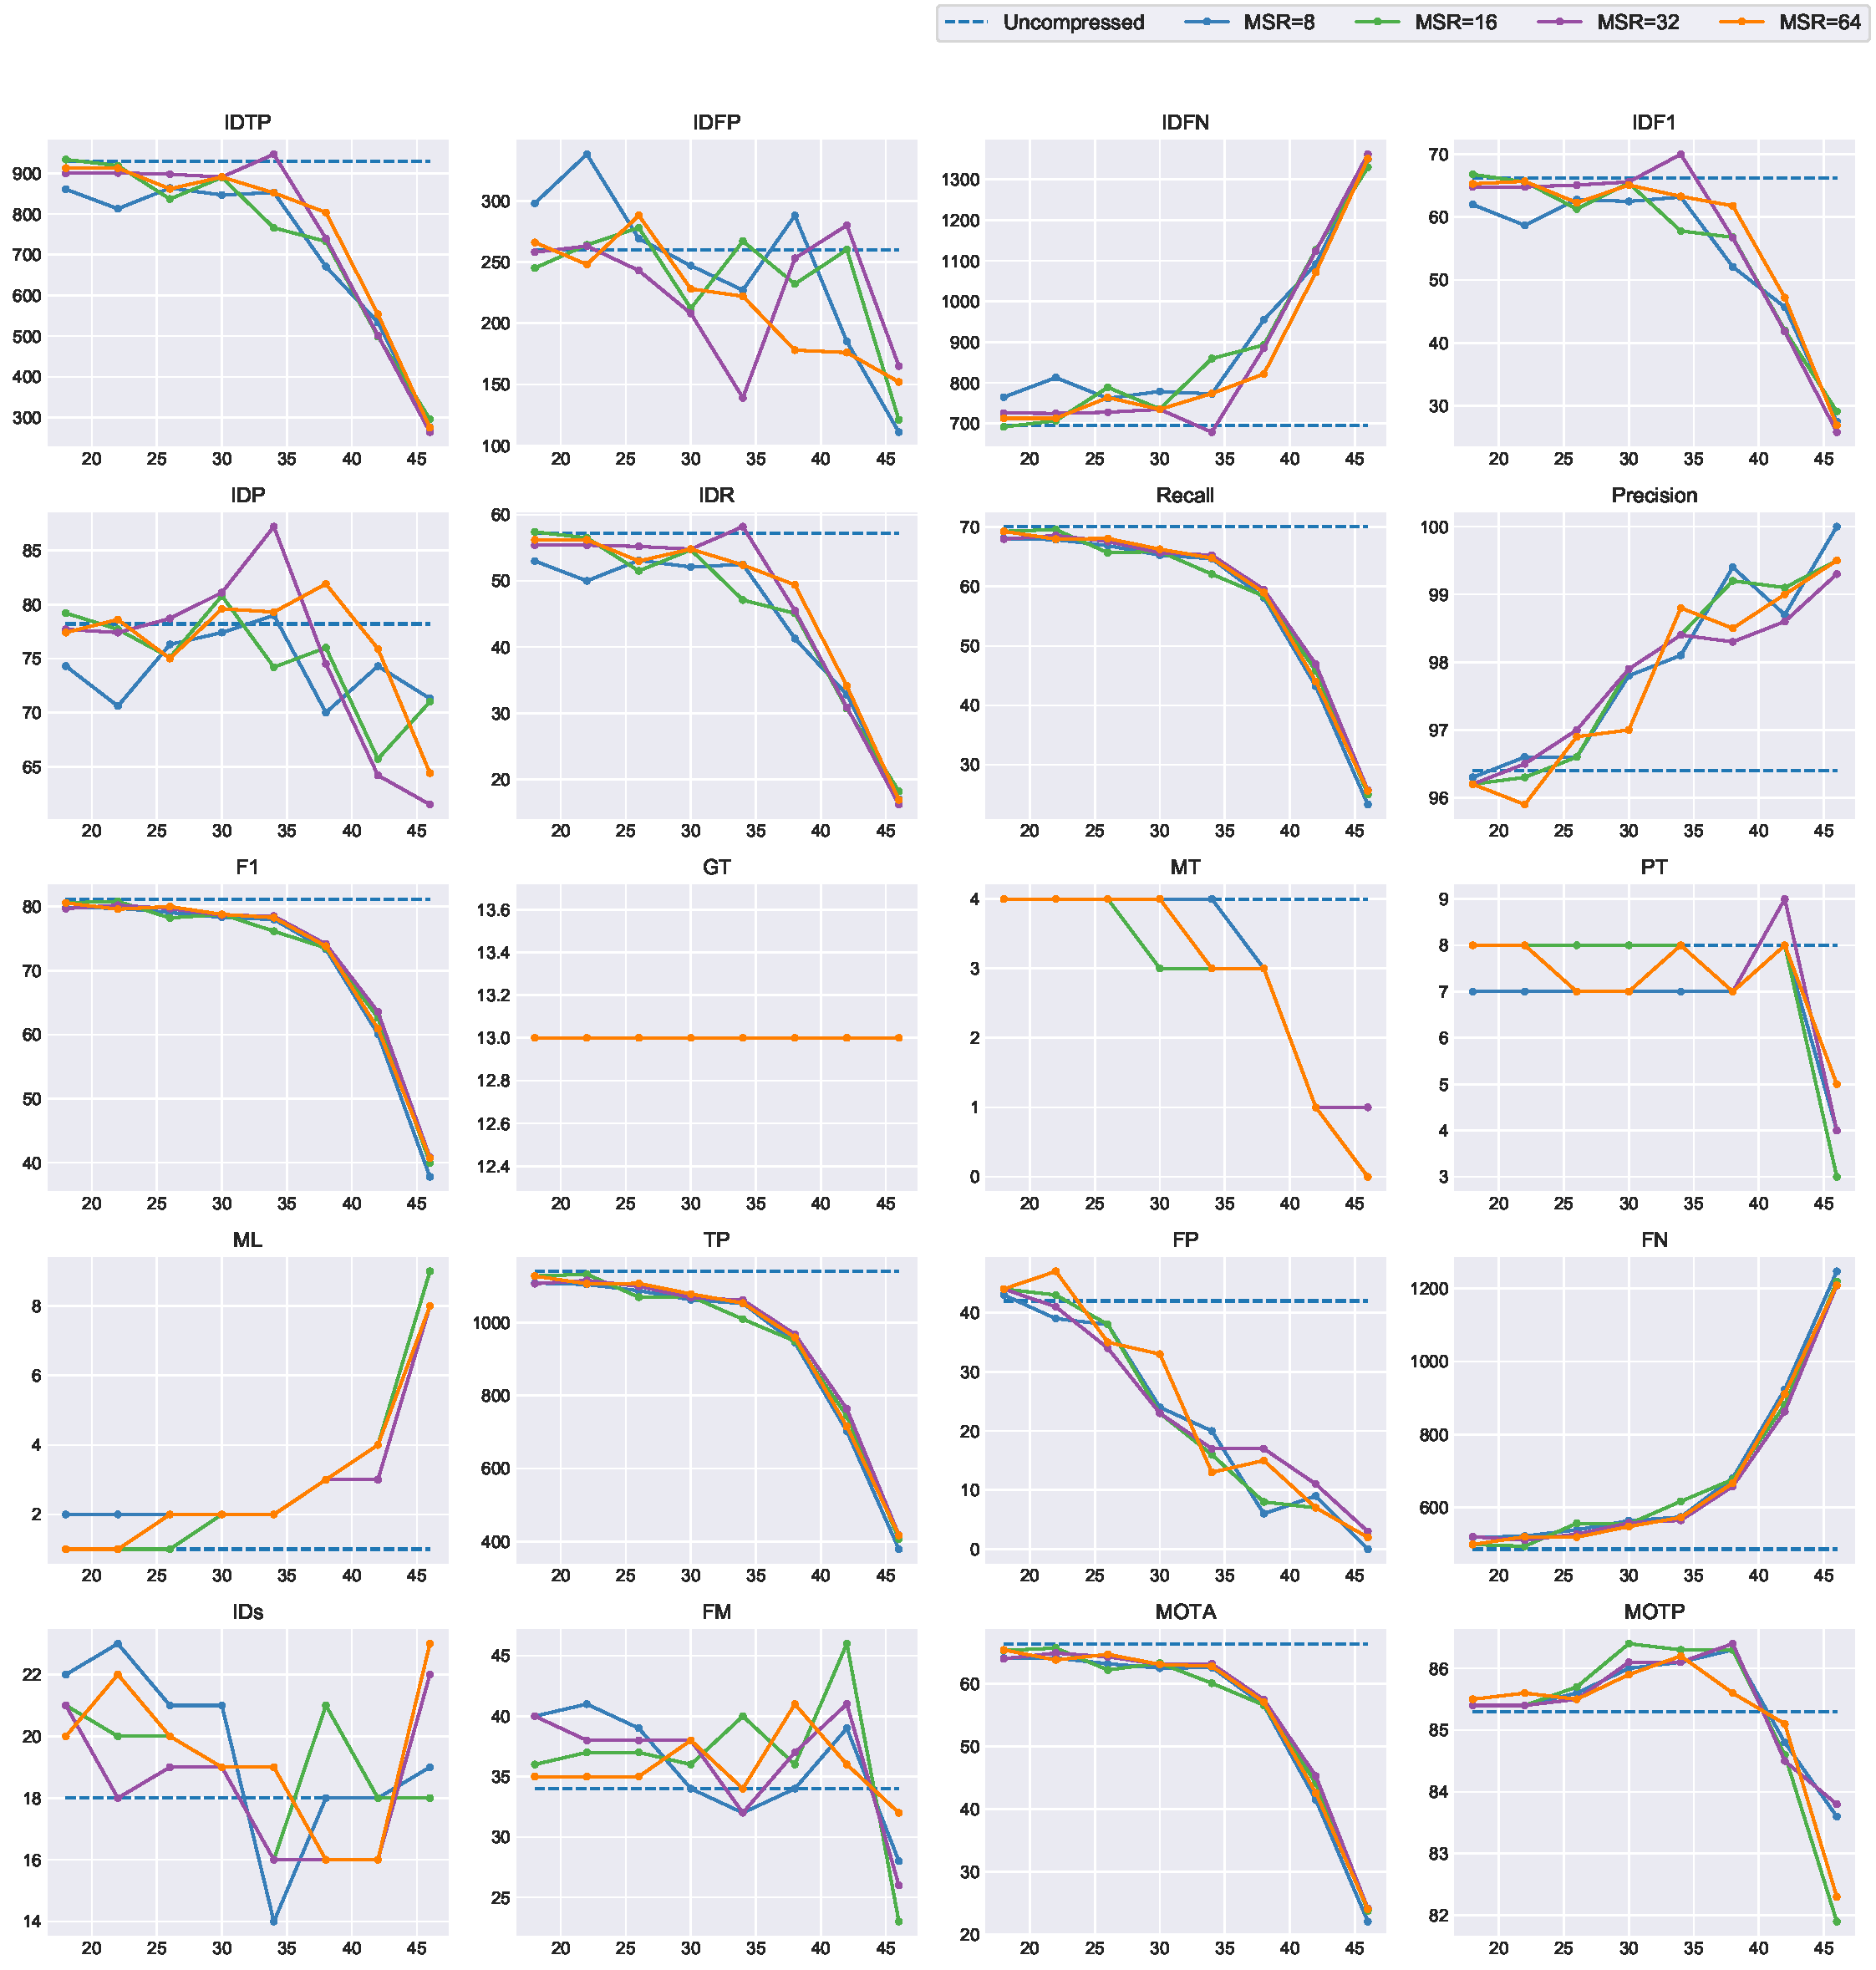
\includegraphics[width=1.0\linewidth]{img/appendix/RaceHorsesC_all_multiplots_qp.pdf}
\caption[Result of all object classes in Class C RaceHorsesC with Horizontal Axis of QP]{}
\label{fig:RaceHorsesC_all_qp}
\end{figure}

\begin{figure}[!htbp]
\centering
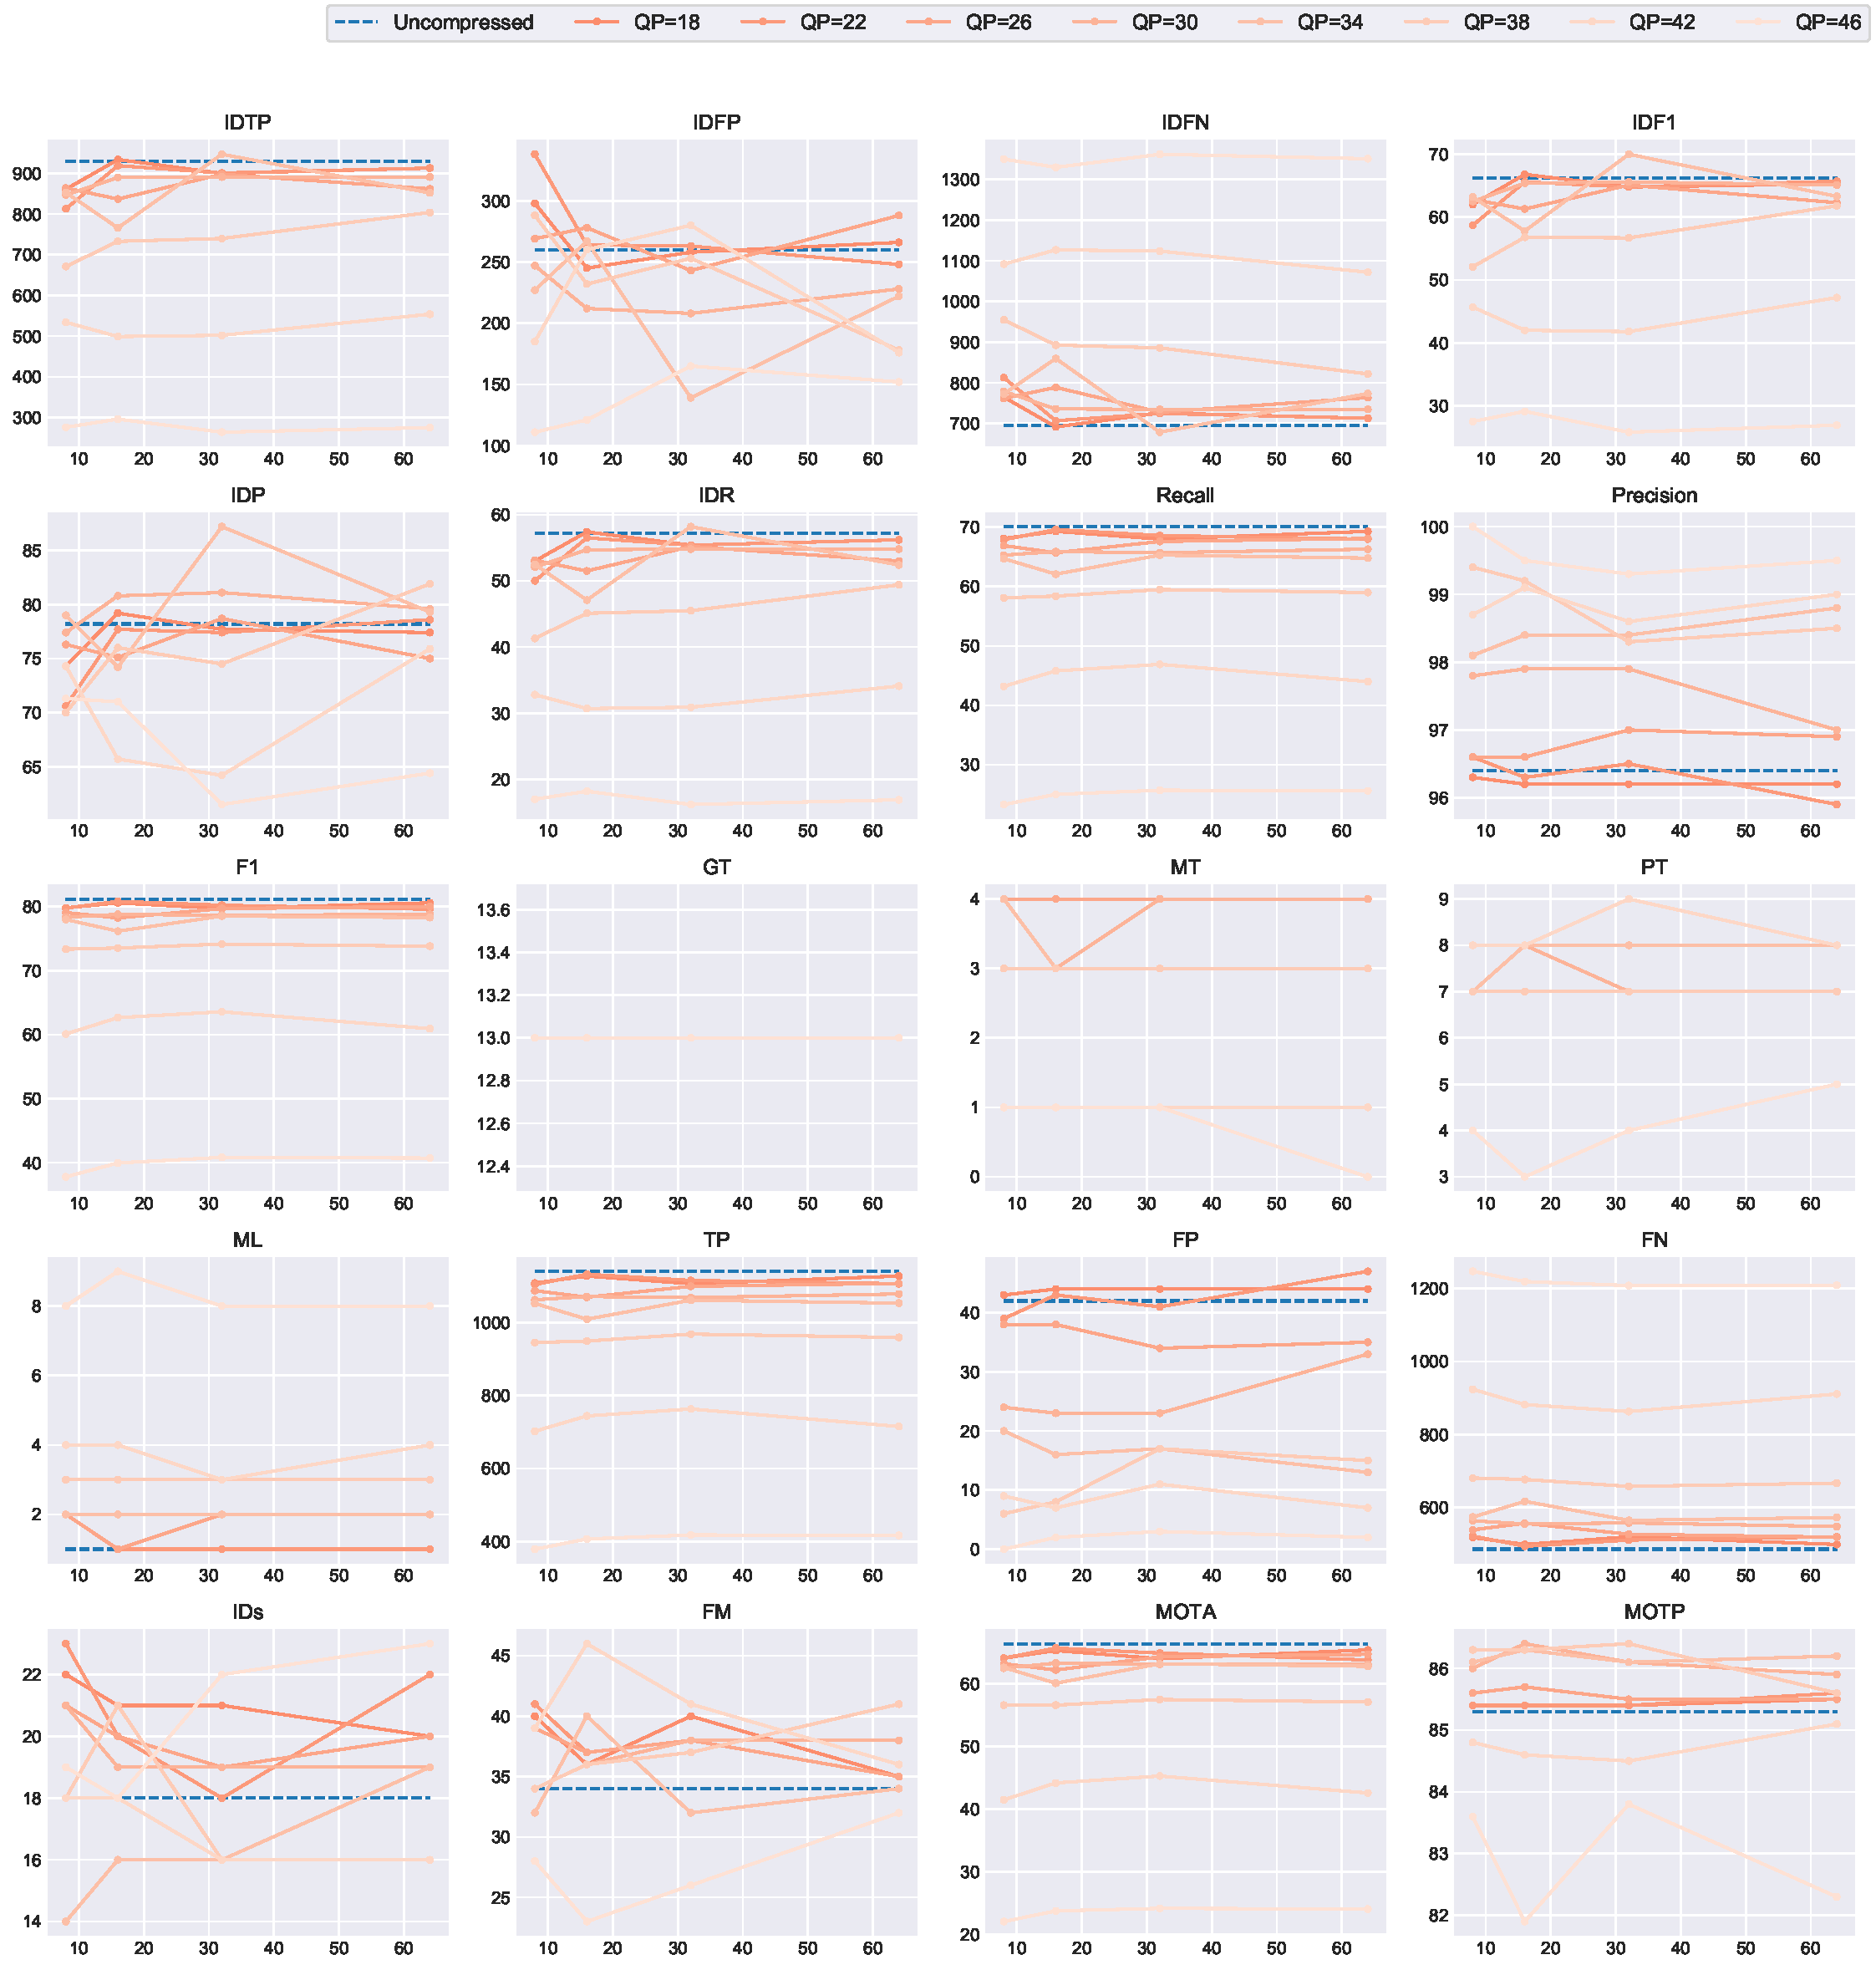
\includegraphics[width=1.0\linewidth]{img/appendix/RaceHorsesC_all_multiplots_msr.pdf}
\caption[Result of all object classes in Class C RaceHorsesC with Horizontal Axis of MSR]{}
\label{fig:RaceHorsesC_all_msr}
\end{figure}



% table
\begin{table}
\centering
\caption{Result of all object classes in Class C RaceHorsesC}


% table for uncompressed
\begin{subtable}[t]{\linewidth}
\centering
\vspace{0pt}
\resizebox{1.0\linewidth}{!}{
\begin{tabular}{llrrrrrrrrrrrrrrrrrrrr}
\toprule
          QP &          MSR &   IDTP &   IDFP &   IDFN &  IDF1 &   IDP &   IDR &  Recall &  Precision &    F1 &  GT &  MT &  PT &  ML &   TP &  FP &  FN &  IDs &  FM &  MOTA &  MOTP \\
\midrule
Uncompressed & Uncompressed & 930.00 & 260.00 & 696.00 & 66.20 & 78.20 & 57.20 &   70.10 &      96.40 & 81.17 &  13 &   4 &   8 &   1 & 1140 &  42 & 486 &   18 &  34 & 66.40 & 85.30 \\
\bottomrule
\end{tabular}

}
\caption{Uncompressed Sequence}
\end{subtable}


% table for msr=8
\begin{subtable}[t]{\linewidth}
\centering
\resizebox{1.0\linewidth}{!}{
\begin{tabular}{rrrrrrrrrrrrrrrrrrrrrr}
\toprule
 QP &  MSR &   IDTP &   IDFP &    IDFN &  IDF1 &   IDP &   IDR &  Recall &  Precision &    F1 &  GT &  MT &  PT &  ML &   TP &  FP &   FN &  IDs &  FM &  MOTA &  MOTP \\
\midrule
 18 &    8 & 861.00 & 298.00 &  765.00 & 62.00 & 74.30 & 53.00 &   68.10 &      96.30 & 79.78 &  13 &   4 &   7 &   2 & 1108 &  43 &  518 &   22 &  40 & 64.10 & 85.40 \\
 22 &    8 & 813.00 & 338.00 &  813.00 & 58.70 & 70.60 & 50.00 &   67.90 &      96.60 & 79.75 &  13 &   4 &   7 &   2 & 1104 &  39 &  522 &   23 &  41 & 64.10 & 85.40 \\
 26 &    8 & 864.00 & 269.00 &  762.00 & 62.80 & 76.30 & 53.10 &   66.90 &      96.60 & 79.05 &  13 &   4 &   7 &   2 & 1087 &  38 &  539 &   21 &  39 & 63.20 & 85.60 \\
 30 &    8 & 847.00 & 247.00 &  779.00 & 62.50 & 77.40 & 52.10 &   65.30 &      97.80 & 78.31 &  13 &   4 &   7 &   2 & 1062 &  24 &  564 &   21 &  34 & 62.50 & 86.00 \\
 34 &    8 & 853.00 & 227.00 &  773.00 & 63.20 & 79.00 & 52.50 &   64.70 &      98.10 & 77.97 &  13 &   4 &   7 &   2 & 1052 &  20 &  574 &   14 &  32 & 62.60 & 86.10 \\
 38 &    8 & 671.00 & 288.00 &  955.00 & 52.10 & 70.00 & 41.30 &   58.10 &      99.40 & 73.34 &  13 &   3 &   7 &   3 &  945 &   6 &  681 &   18 &  34 & 56.60 & 86.30 \\
 42 &    8 & 534.00 & 185.00 & 1092.00 & 45.70 & 74.30 & 32.80 &   43.20 &      98.70 & 60.10 &  13 &   1 &   8 &   4 &  702 &   9 &  924 &   18 &  39 & 41.50 & 84.80 \\
 46 &    8 & 276.00 & 111.00 & 1350.00 & 27.50 & 71.30 & 17.00 &   23.30 &     100.00 & 37.79 &  13 &   1 &   4 &   8 &  379 &   0 & 1247 &   19 &  28 & 22.10 & 83.60 \\
\bottomrule
\end{tabular}

}
\caption{MSR = 8}
\end{subtable}



% table for msr=16
\begin{subtable}[t]{\linewidth}
\centering
\resizebox{1.0\linewidth}{!}{
\begin{tabular}{rrrrrrrrrrrrrrrrrrrrrr}
\toprule
 QP &  MSR &   IDTP &   IDFP &    IDFN &  IDF1 &   IDP &   IDR &  Recall &  Precision &    F1 &  GT &  MT &  PT &  ML &   TP &  FP &   FN &  IDs &  FM &  MOTA &  MOTP \\
\midrule
 18 &   16 & 934.00 & 245.00 &  692.00 & 66.80 & 79.20 & 57.40 &   69.30 &      96.20 & 80.56 &  13 &   4 &   8 &   1 & 1127 &  44 &  499 &   21 &  36 & 65.30 & 85.40 \\
 22 &   16 & 919.00 & 264.00 &  707.00 & 65.60 & 77.70 & 56.50 &   69.60 &      96.30 & 80.80 &  13 &   4 &   8 &   1 & 1132 &  43 &  494 &   20 &  37 & 65.70 & 85.40 \\
 26 &   16 & 837.00 & 278.00 &  789.00 & 61.30 & 75.10 & 51.50 &   65.70 &      96.60 & 78.21 &  13 &   4 &   8 &   1 & 1069 &  38 &  557 &   20 &  37 & 62.20 & 85.70 \\
 30 &   16 & 890.00 & 212.00 &  736.00 & 65.40 & 80.80 & 54.70 &   65.90 &      97.90 & 78.77 &  13 &   3 &   8 &   2 & 1071 &  23 &  555 &   19 &  36 & 63.30 & 86.40 \\
 34 &   16 & 766.00 & 267.00 &  860.00 & 57.80 & 74.20 & 47.10 &   62.10 &      98.40 & 76.15 &  13 &   3 &   8 &   2 & 1009 &  16 &  617 &   16 &  40 & 60.10 & 86.30 \\
 38 &   16 & 733.00 & 232.00 &  893.00 & 56.80 & 76.00 & 45.10 &   58.40 &      99.20 & 73.52 &  13 &   3 &   7 &   3 &  949 &   8 &  677 &   21 &  36 & 56.60 & 86.30 \\
 42 &   16 & 499.00 & 260.00 & 1127.00 & 42.00 & 65.70 & 30.70 &   45.80 &      99.10 & 62.65 &  13 &   1 &   8 &   4 &  744 &   7 &  882 &   18 &  46 & 44.20 & 84.60 \\
 46 &   16 & 296.00 & 121.00 & 1330.00 & 29.10 & 71.00 & 18.20 &   25.00 &      99.50 & 39.96 &  13 &   1 &   3 &   9 &  407 &   2 & 1219 &   18 &  23 & 23.80 & 81.90 \\
\bottomrule
\end{tabular}

}
\caption{MSR = 16}
\end{subtable}


% table for msr=32
\begin{subtable}[t]{\linewidth}
\centering
\resizebox{1.0\linewidth}{!}{
\begin{tabular}{rrrrrrrrrrrrrrrrrrrrrr}
\toprule
 QP &  MSR &   IDTP &   IDFP &    IDFN &  IDF1 &   IDP &   IDR &  Recall &  Precision &    F1 &  GT &  MT &  PT &  ML &   TP &  FP &   FN &  IDs &  FM &  MOTA &  MOTP \\
\midrule
 18 &   32 & 900.00 & 258.00 &  726.00 & 64.80 & 77.70 & 55.40 &   68.00 &      96.20 & 79.68 &  13 &   4 &   8 &   1 & 1106 &  44 &  520 &   21 &  40 & 64.00 & 85.40 \\
 22 &   32 & 901.00 & 263.00 &  725.00 & 64.80 & 77.40 & 55.40 &   68.60 &      96.50 & 80.19 &  13 &   4 &   8 &   1 & 1115 &  41 &  511 &   18 &  38 & 64.90 & 85.40 \\
 26 &   32 & 898.00 & 243.00 &  728.00 & 65.10 & 78.70 & 55.20 &   67.60 &      97.00 & 79.67 &  13 &   4 &   7 &   2 & 1099 &  34 &  527 &   19 &  38 & 64.30 & 85.50 \\
 30 &   32 & 891.00 & 208.00 &  735.00 & 65.60 & 81.10 & 54.80 &   65.70 &      97.90 & 78.63 &  13 &   4 &   7 &   2 & 1068 &  23 &  558 &   19 &  38 & 63.10 & 86.10 \\
 34 &   32 & 947.00 & 139.00 &  679.00 & 70.00 & 87.20 & 58.20 &   65.30 &      98.40 & 78.50 &  13 &   3 &   8 &   2 & 1061 &  17 &  565 &   16 &  32 & 63.20 & 86.10 \\
 38 &   32 & 740.00 & 253.00 &  886.00 & 56.70 & 74.50 & 45.50 &   59.50 &      98.30 & 74.13 &  13 &   3 &   7 &   3 &  968 &  17 &  658 &   16 &  37 & 57.50 & 86.40 \\
 42 &   32 & 502.00 & 280.00 & 1124.00 & 41.80 & 64.20 & 30.90 &   46.90 &      98.60 & 63.56 &  13 &   1 &   9 &   3 &  763 &  11 &  863 &   16 &  41 & 45.30 & 84.50 \\
 46 &   32 & 264.00 & 165.00 & 1362.00 & 25.80 & 61.50 & 16.20 &   25.70 &      99.30 & 40.83 &  13 &   1 &   4 &   8 &  418 &   3 & 1208 &   22 &  26 & 24.20 & 83.80 \\
\bottomrule
\end{tabular}

}
\caption{MSR = 32}
\end{subtable}


% table for msr=64
\begin{subtable}[t]{\linewidth}
\centering
\resizebox{1.0\linewidth}{!}{
\begin{tabular}{rrrrrrrrrrrrrrrrrrrrrr}
\toprule
 QP &  MSR &   IDTP &   IDFP &    IDFN &  IDF1 &   IDP &   IDR &  Recall &  Precision &    F1 &  GT &  MT &  PT &  ML &   TP &  FP &   FN &  IDs &  FM &  MOTA &  MOTP \\
\midrule
 18 &   64 & 913.00 & 266.00 &  713.00 & 65.30 & 77.40 & 56.20 &   69.30 &      96.20 & 80.56 &  13 &   4 &   8 &   1 & 1127 &  44 &  499 &   20 &  35 & 65.40 & 85.50 \\
 22 &   64 & 913.00 & 248.00 &  713.00 & 65.70 & 78.60 & 56.20 &   68.00 &      95.90 & 79.58 &  13 &   4 &   8 &   1 & 1106 &  47 &  520 &   22 &  35 & 63.80 & 85.60 \\
 26 &   64 & 862.00 & 288.00 &  764.00 & 62.30 & 75.00 & 53.00 &   68.10 &      96.90 & 79.99 &  13 &   4 &   7 &   2 & 1107 &  35 &  519 &   20 &  35 & 64.70 & 85.50 \\
 30 &   64 & 891.00 & 228.00 &  735.00 & 65.10 & 79.60 & 54.80 &   66.30 &      97.00 & 78.76 &  13 &   4 &   7 &   2 & 1078 &  33 &  548 &   19 &  38 & 63.10 & 85.90 \\
 34 &   64 & 852.00 & 222.00 &  774.00 & 63.30 & 79.30 & 52.40 &   64.80 &      98.80 & 78.27 &  13 &   3 &   8 &   2 & 1053 &  13 &  573 &   19 &  34 & 62.80 & 86.20 \\
 38 &   64 & 804.00 & 178.00 &  822.00 & 61.80 & 81.90 & 49.40 &   59.00 &      98.50 & 73.80 &  13 &   3 &   7 &   3 &  959 &  15 &  667 &   16 &  41 & 57.10 & 85.60 \\
 42 &   64 & 554.00 & 176.00 & 1072.00 & 47.20 & 75.90 & 34.10 &   44.00 &      99.00 & 60.92 &  13 &   1 &   8 &   4 &  715 &   7 &  911 &   16 &  36 & 42.60 & 85.10 \\
 46 &   64 & 275.00 & 152.00 & 1351.00 & 26.90 & 64.40 & 16.90 &   25.60 &      99.50 & 40.72 &  13 &   0 &   5 &   8 &  417 &   2 & 1209 &   23 &  32 & 24.10 & 82.30 \\
\bottomrule
\end{tabular}

}
\caption{MSR = 64}
\end{subtable}


\label{tab:RaceHorsesC_all}
\end{table}




\begin{table}[!htbp]
\centering
\caption{Multiple Linear Regression Analysis Result for Class C RaceHorsesC}
\resizebox{1.0\linewidth}{!}{
\begin{tabular}{lrrrrrrrrrrrrrrrrrrr}
\toprule
{} &    IDTP &   IDFP &   IDFN &  IDF1 &   IDP &   IDR &  Recall &  Precision &     F1 &    MT &    PT &    ML &      TP &    FP &     FN &   IDs &    FM &  MOTA &  MOTP \\
\midrule
coefficient(Intercept) & 1344.71 & 375.50 & 281.29 & 90.44 & 82.15 & 82.68 &  100.75 &      93.82 & 108.98 &  6.56 &  9.48 & -3.04 & 1638.53 & 73.69 & -12.53 & 23.82 & 46.56 & 94.73 & 86.95 \\
coefficient(QP)        &  -19.53 &  -4.11 &  19.53 & -1.12 & -0.25 & -1.20 &   -1.35 &       0.13 &  -1.19 & -0.11 & -0.08 &  0.19 &  -22.03 & -1.61 &  22.03 & -0.15 & -0.32 & -1.25 & -0.05 \\
coefficient(MSR)       &    0.82 &  -0.75 &  -0.82 &  0.05 &  0.10 &  0.05 &    0.00 &      -0.00 &  -0.01 &  0.01 & -0.00 & -0.01 &    0.01 &  0.06 &  -0.01 & -0.06 & -0.15 &  0.00 &  0.01 \\
coefficient(QP*MSR)    &   -0.00 &   0.01 &   0.00 & -0.00 & -0.00 & -0.00 &    0.00 &      -0.00 &   0.00 & -0.00 &  0.00 &  0.00 &    0.01 & -0.00 &  -0.01 &  0.00 &  0.00 &  0.00 & -0.00 \\
p-value(Intercept)     &    0.00 &   0.00 &   0.05 &  0.00 &  0.00 &  0.00 &    0.00 &       0.00 &   0.00 &  0.00 &  0.00 &  0.06 &    0.00 &  0.00 &   0.93 &  0.00 &  0.00 &  0.00 &  0.00 \\
p-value(QP)            &    0.00 &   0.01 &   0.00 &  0.00 &  0.14 &  0.00 &    0.00 &       0.00 &   0.00 &  0.00 &  0.06 &  0.00 &    0.00 &  0.00 &   0.00 &  0.06 &  0.03 &  0.00 &  0.15 \\
p-value(MSR)           &    0.83 &   0.56 &   0.83 &  0.83 &  0.53 &  0.82 &    1.00 &       0.80 &   0.96 &  0.57 &  0.95 &  0.83 &    1.00 &  0.61 &   1.00 &  0.41 &  0.26 &  1.00 &  0.81 \\
p-value(QP*MSR)        &    0.97 &   0.79 &   0.97 &  0.98 &  0.70 &  0.97 &    0.96 &       0.93 &   0.92 &  0.46 &  0.81 &  0.88 &    0.95 &  0.86 &   0.95 &  0.40 &  0.26 &  0.96 &  0.74 \\
\bottomrule
\end{tabular}

}
\label{tab:RaceHorsesC_all_reg}
\end{table}



\newpage

\section{BasketballPass}
\label{sec:appendix/BasketballPass_all}


% visualization figure
\begin{figure}[!htbp]
\centering
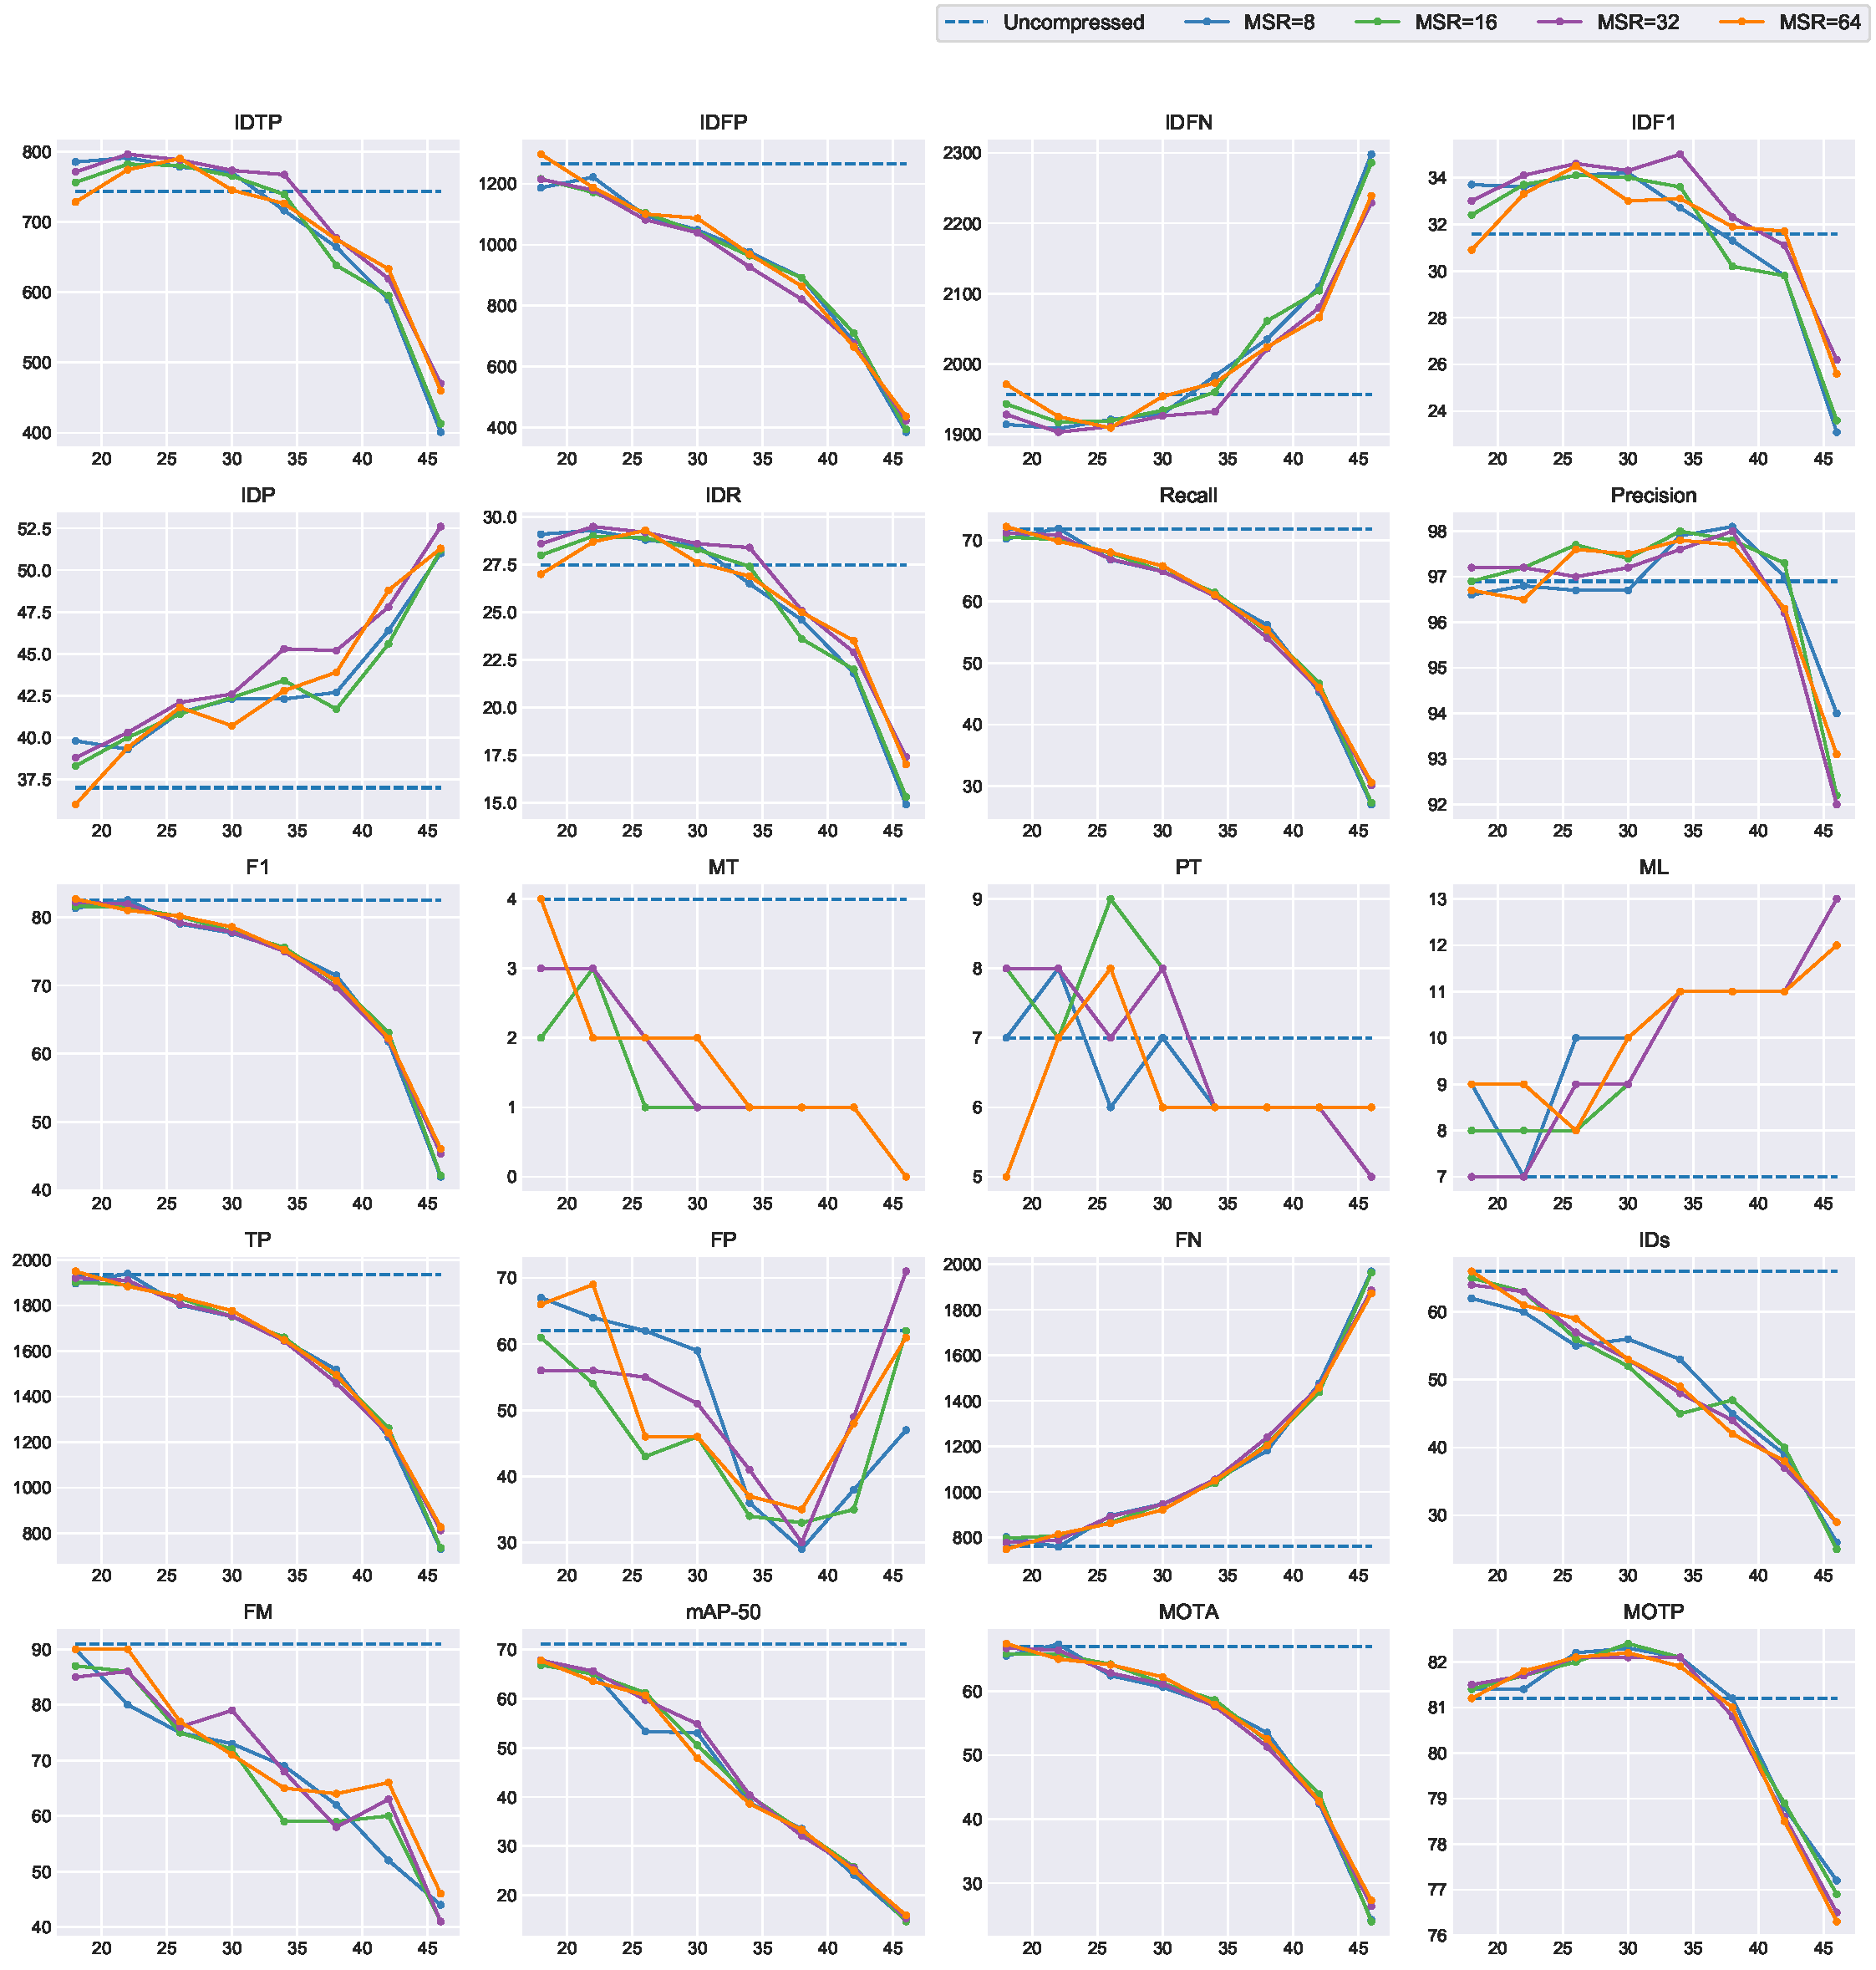
\includegraphics[width=1.0\linewidth]{img/appendix/BasketballPass_all_multiplots_qp.pdf}
\caption[Visualization of performance results on BasketballPass at different QP]
{Visualization of performance results on BasketballPass at different QP.}
\label{fig:BasketballPass_all_qp}
\end{figure}

\begin{figure}[!htbp]
\centering
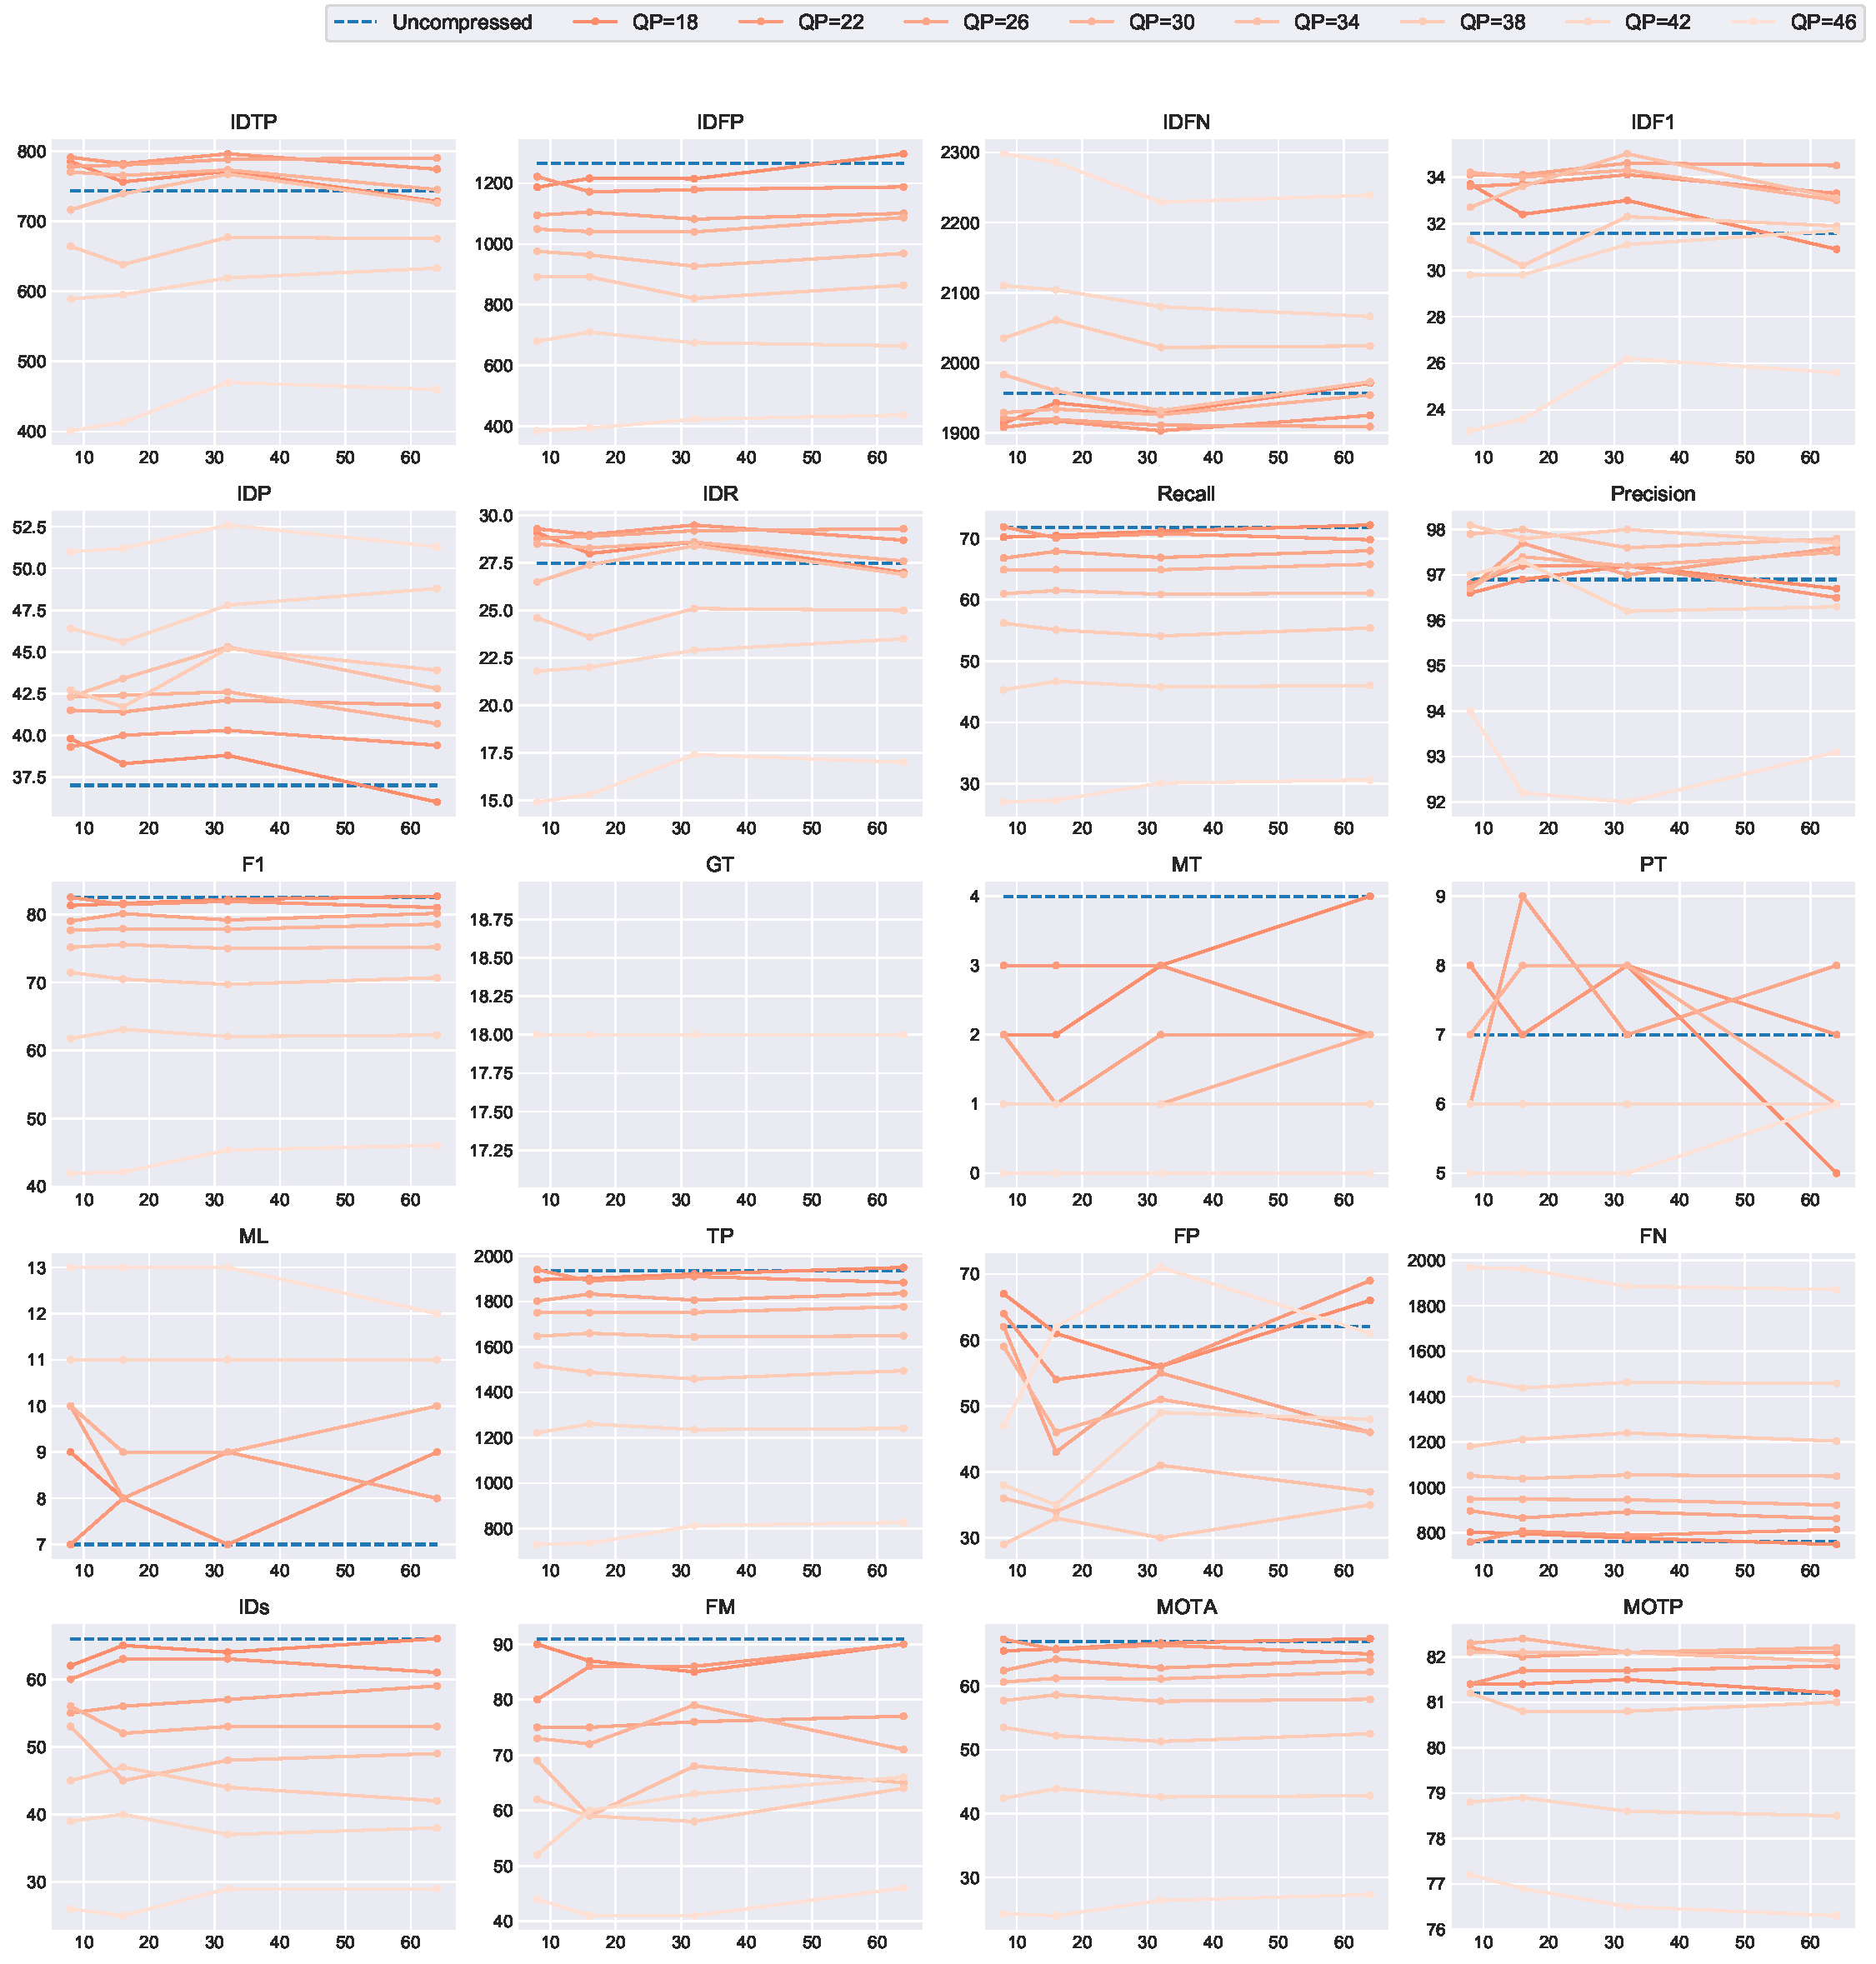
\includegraphics[width=1.0\linewidth]{img/appendix/BasketballPass_all_multiplots_msr.pdf}
\caption[Visualization of performance results on BasketballPass at different MSR]
{Visualization of performance results on BasketballPass at different MSR.}
\label{fig:BasketballPass_all_msr}
\end{figure}



% table
\begin{table}
\centering
\caption[Performance results on BasketballPass]
{Performance results on BasketballPass.}


% table for uncompressed
\begin{subtable}[t]{\linewidth}
\centering
\vspace{0pt}
\resizebox{1.0\linewidth}{!}{
\begin{tabular}{llrrrrrrrrrrrrrrrrrrrrr}
\toprule
          QP &          MSR &   IDTP &    IDFP &    IDFN &  IDF1 &   IDP &   IDR &  Recall &  Precision &    F1 &  GT &  MT &  PT &  ML &   TP &  FP &  FN &  IDs &  FM &  mAP-50 &  MOTA &  MOTP \\
\midrule
Uncompressed & Uncompressed & 743.00 & 1265.00 & 1956.00 & 31.60 & 37.00 & 27.50 &   71.80 &      96.90 & 82.48 &  18 &   4 &   7 &   7 & 1937 &  62 & 762 &   66 &  91 &   71.22 & 67.00 & 81.20 \\
\bottomrule
\end{tabular}

}
\caption{Uncompressed Sequence}
\end{subtable}


% table for msr=8
\begin{subtable}[t]{\linewidth}
\centering
\resizebox{1.0\linewidth}{!}{
\begin{tabular}{rrrrrrrrrrrrrrrrrrrrrrr}
\toprule
 QP &  MSR &   IDTP &    IDFP &    IDFN &  IDF1 &   IDP &   IDR &  Recall &  Precision &    F1 &  GT &  MT &  PT &  ML &   TP &  FP &   FN &  IDs &  FM &  mAP-50 &  MOTA &  MOTP \\
\midrule
 18 &    8 & 785.00 & 1187.00 & 1914.00 & 33.70 & 39.80 & 29.10 &   70.20 &      96.60 & 81.31 &  18 &   2 &   7 &   9 & 1896 &  67 &  803 &   62 &  90 &   66.81 & 65.50 & 81.40 \\
 22 &    8 & 791.00 & 1222.00 & 1908.00 & 33.60 & 39.30 & 29.30 &   71.90 &      96.80 & 82.51 &  18 &   3 &   8 &   7 & 1940 &  64 &  759 &   60 &  80 &   65.50 & 67.30 & 81.40 \\
 26 &    8 & 778.00 & 1095.00 & 1921.00 & 34.10 & 41.50 & 28.80 &   66.80 &      96.70 & 79.02 &  18 &   2 &   6 &  10 & 1802 &  62 &  897 &   55 &  75 &   53.38 & 62.40 & 82.20 \\
 30 &    8 & 770.00 & 1049.00 & 1929.00 & 34.20 & 42.30 & 28.50 &   64.90 &      96.70 & 77.67 &  18 &   1 &   7 &  10 & 1751 &  59 &  948 &   56 &  73 &   53.01 & 60.60 & 82.30 \\
 34 &    8 & 716.00 &  976.00 & 1983.00 & 32.70 & 42.30 & 26.50 &   61.00 &      97.90 & 75.17 &  18 &   1 &   6 &  11 & 1647 &  36 & 1052 &   53 &  69 &   38.80 & 57.70 & 82.10 \\
 38 &    8 & 664.00 &  892.00 & 2035.00 & 31.30 & 42.70 & 24.60 &   56.20 &      98.10 & 71.46 &  18 &   1 &   6 &  11 & 1518 &  29 & 1181 &   45 &  62 &   33.54 & 53.50 & 81.20 \\
 42 &    8 & 589.00 &  680.00 & 2110.00 & 29.80 & 46.40 & 21.80 &   45.30 &      97.00 & 61.76 &  18 &   1 &   6 &  11 & 1222 &  38 & 1477 &   39 &  52 &   24.14 & 42.40 & 78.80 \\
 46 &    8 & 401.00 &  385.00 & 2298.00 & 23.10 & 51.00 & 14.90 &   27.00 &      94.00 & 41.95 &  18 &   0 &   5 &  13 &  730 &  47 & 1969 &   26 &  44 &   14.91 & 24.30 & 77.20 \\
\bottomrule
\end{tabular}

}
\caption{MSR = 8}
\end{subtable}



% table for msr=16
\begin{subtable}[t]{\linewidth}
\centering
\resizebox{1.0\linewidth}{!}{
\begin{tabular}{rrrrrrrrrrrrrrrrrrrrrrr}
\toprule
 QP &  MSR &   IDTP &    IDFP &    IDFN &  IDF1 &   IDP &   IDR &  Recall &  Precision &    F1 &  GT &  MT &  PT &  ML &   TP &  FP &   FN &  IDs &  FM &  mAP-50 &  MOTA &  MOTP \\
\midrule
 18 &   16 & 756.00 & 1216.00 & 1943.00 & 32.40 & 38.30 & 28.00 &   70.50 &      96.90 & 81.62 &  18 &   2 &   8 &   8 & 1902 &  61 &  797 &   65 &  87 &   66.87 & 65.80 & 81.40 \\
 22 &   16 & 782.00 & 1172.00 & 1917.00 & 33.70 & 40.00 & 29.00 &   70.10 &      97.20 & 81.46 &  18 &   3 &   7 &   8 & 1891 &  54 &  808 &   63 &  86 &   65.05 & 65.70 & 81.70 \\
 26 &   16 & 780.00 & 1105.00 & 1919.00 & 34.10 & 41.40 & 28.90 &   67.90 &      97.70 & 80.12 &  18 &   1 &   9 &   8 & 1833 &  43 &  866 &   56 &  75 &   61.21 & 64.20 & 82.00 \\
 30 &   16 & 765.00 & 1041.00 & 1934.00 & 34.00 & 42.40 & 28.30 &   64.90 &      97.40 & 77.90 &  18 &   1 &   8 &   9 & 1751 &  46 &  948 &   52 &  72 &   50.56 & 61.20 & 82.40 \\
 34 &   16 & 739.00 &  964.00 & 1960.00 & 33.60 & 43.40 & 27.40 &   61.50 &      98.00 & 75.57 &  18 &   1 &   6 &  11 & 1660 &  34 & 1039 &   45 &  59 &   40.22 & 58.60 & 82.10 \\
 38 &   16 & 638.00 &  892.00 & 2061.00 & 30.20 & 41.70 & 23.60 &   55.10 &      97.80 & 70.49 &  18 &   1 &   6 &  11 & 1488 &  33 & 1211 &   47 &  59 &   33.09 & 52.20 & 80.80 \\
 42 &   16 & 595.00 &  710.00 & 2104.00 & 29.80 & 45.60 & 22.00 &   46.70 &      97.30 & 63.11 &  18 &   1 &   6 &  11 & 1261 &  35 & 1438 &   40 &  60 &   25.78 & 43.90 & 78.90 \\
 46 &   16 & 413.00 &  394.00 & 2286.00 & 23.60 & 51.20 & 15.30 &   27.30 &      92.20 & 42.13 &  18 &   0 &   5 &  13 &  736 &  62 & 1963 &   25 &  41 &   14.65 & 24.00 & 76.90 \\
\bottomrule
\end{tabular}

}
\caption{MSR = 16}
\end{subtable}


% table for msr=32
\begin{subtable}[t]{\linewidth}
\centering
\resizebox{1.0\linewidth}{!}{
\begin{tabular}{rrrrrrrrrrrrrrrrrrrrrrr}
\toprule
 QP &  MSR &   IDTP &    IDFP &    IDFN &  IDF1 &   IDP &   IDR &  Recall &  Precision &    F1 &  GT &  MT &  PT &  ML &   TP &  FP &   FN &  IDs &  FM &  mAP-50 &  MOTA &  MOTP \\
\midrule
 18 &   32 & 771.00 & 1215.00 & 1928.00 & 33.00 & 38.80 & 28.60 &   71.20 &      97.20 & 82.19 &  18 &   3 &   8 &   7 & 1921 &  56 &  778 &   64 &  85 &   67.85 & 66.70 & 81.50 \\
 22 &   32 & 796.00 & 1179.00 & 1903.00 & 34.10 & 40.30 & 29.50 &   70.80 &      97.20 & 81.93 &  18 &   3 &   8 &   7 & 1910 &  56 &  789 &   63 &  86 &   65.63 & 66.40 & 81.70 \\
 26 &   32 & 788.00 & 1082.00 & 1911.00 & 34.60 & 42.10 & 29.20 &   66.90 &      97.00 & 79.19 &  18 &   2 &   7 &   9 & 1806 &  55 &  893 &   57 &  76 &   59.75 & 62.80 & 82.10 \\
 30 &   32 & 773.00 & 1040.00 & 1926.00 & 34.30 & 42.60 & 28.60 &   64.90 &      97.20 & 77.83 &  18 &   1 &   8 &   9 & 1753 &  51 &  946 &   53 &  79 &   54.88 & 61.10 & 82.10 \\
 34 &   32 & 767.00 &  927.00 & 1932.00 & 35.00 & 45.30 & 28.40 &   60.90 &      97.60 & 75.00 &  18 &   1 &   6 &  11 & 1644 &  41 & 1055 &   48 &  68 &   40.40 & 57.60 & 82.10 \\
 38 &   32 & 677.00 &  821.00 & 2022.00 & 32.30 & 45.20 & 25.10 &   54.10 &      98.00 & 69.71 &  18 &   1 &   6 &  11 & 1459 &  30 & 1240 &   44 &  58 &   32.11 & 51.30 & 80.80 \\
 42 &   32 & 619.00 &  675.00 & 2080.00 & 31.10 & 47.80 & 22.90 &   45.80 &      96.20 & 62.06 &  18 &   1 &   6 &  11 & 1236 &  49 & 1463 &   37 &  63 &   25.54 & 42.60 & 78.60 \\
 46 &   32 & 470.00 &  423.00 & 2229.00 & 26.20 & 52.60 & 17.40 &   30.10 &      92.00 & 45.36 &  18 &   0 &   5 &  13 &  813 &  71 & 1886 &   29 &  41 &   15.31 & 26.40 & 76.50 \\
\bottomrule
\end{tabular}

}
\caption{MSR = 32}
\end{subtable}


% table for msr=64
\begin{subtable}[t]{\linewidth}
\centering
\resizebox{1.0\linewidth}{!}{
\begin{tabular}{rrrrrrrrrrrrrrrrrrrrrrr}
\toprule
 QP &  MSR &   IDTP &    IDFP &    IDFN &  IDF1 &   IDP &   IDR &  Recall &  Precision &    F1 &  GT &  MT &  PT &  ML &   TP &  FP &   FN &  IDs &  FM &  mAP-50 &  MOTA &  MOTP \\
\midrule
 18 &   64 & 728.00 & 1297.00 & 1971.00 & 30.90 & 36.00 & 27.00 &   72.20 &      96.70 & 82.67 &  18 &   4 &   5 &   9 & 1950 &  66 &  749 &   66 &  90 &   67.78 & 67.40 & 81.20 \\
 22 &   64 & 774.00 & 1188.00 & 1925.00 & 33.30 & 39.40 & 28.70 &   69.80 &      96.50 & 81.01 &  18 &   2 &   7 &   9 & 1884 &  69 &  815 &   61 &  90 &   63.57 & 65.00 & 81.80 \\
 26 &   64 & 790.00 & 1101.00 & 1909.00 & 34.50 & 41.80 & 29.30 &   68.00 &      97.60 & 80.15 &  18 &   2 &   8 &   8 & 1836 &  46 &  863 &   59 &  77 &   60.72 & 64.10 & 82.10 \\
 30 &   64 & 745.00 & 1087.00 & 1954.00 & 33.00 & 40.70 & 27.60 &   65.80 &      97.50 & 78.57 &  18 &   2 &   6 &  10 & 1777 &  46 &  922 &   53 &  71 &   47.94 & 62.20 & 82.20 \\
 34 &   64 & 726.00 &  969.00 & 1973.00 & 33.10 & 42.80 & 26.90 &   61.10 &      97.80 & 75.21 &  18 &   1 &   6 &  11 & 1649 &  37 & 1050 &   49 &  65 &   38.64 & 57.90 & 81.90 \\
 38 &   64 & 675.00 &  864.00 & 2024.00 & 31.90 & 43.90 & 25.00 &   55.40 &      97.70 & 70.71 &  18 &   1 &   6 &  11 & 1495 &  35 & 1204 &   42 &  64 &   33.35 & 52.50 & 81.00 \\
 42 &   64 & 633.00 &  665.00 & 2066.00 & 31.70 & 48.80 & 23.50 &   46.00 &      96.30 & 62.26 &  18 &   1 &   6 &  11 & 1241 &  48 & 1458 &   38 &  66 &   25.03 & 42.80 & 78.50 \\
 46 &   64 & 460.00 &  437.00 & 2239.00 & 25.60 & 51.30 & 17.00 &   30.60 &      93.10 & 46.06 &  18 &   0 &   6 &  12 &  827 &  61 & 1872 &   29 &  46 &   15.94 & 27.30 & 76.30 \\
\bottomrule
\end{tabular}

}
\caption{MSR = 64}
\end{subtable}


\label{tab:BasketballPass_all}
\end{table}



\newpage

\section{Class D BlowingBubbles}
\label{sec:appendix/BlowingBubbles_all}


% visualization figure
\begin{figure}[!htbp]
\centering
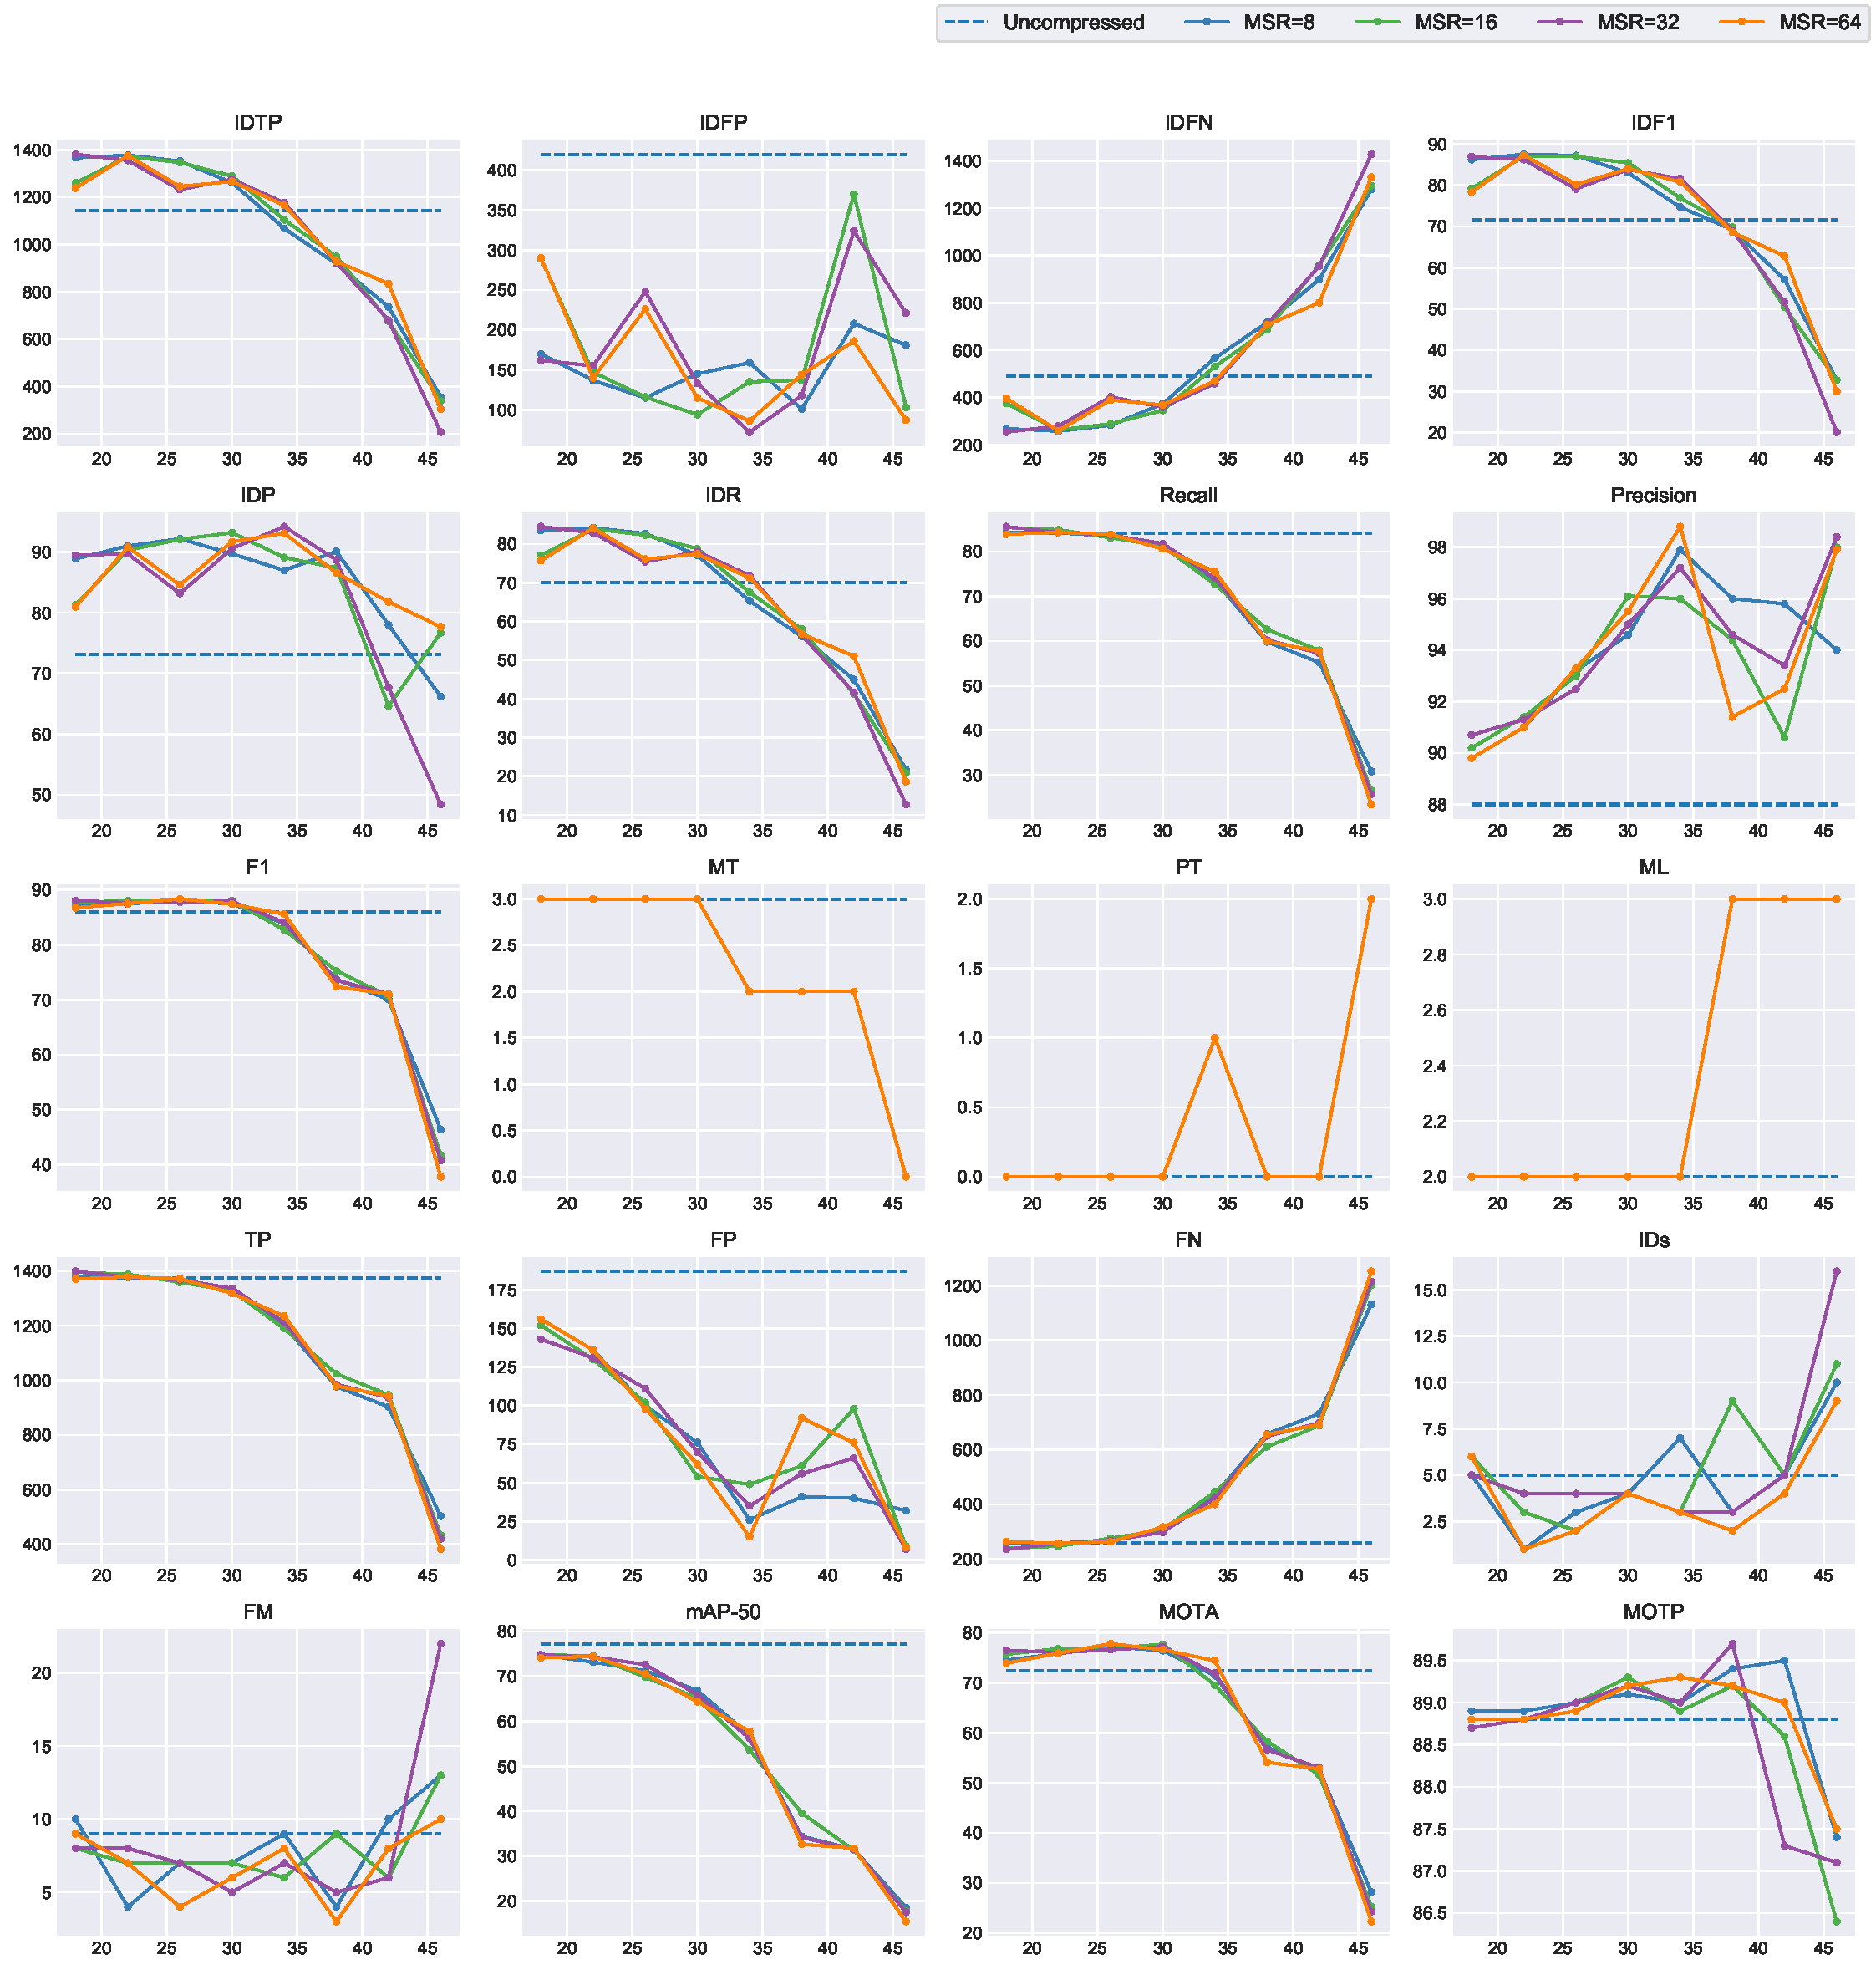
\includegraphics[width=1.0\linewidth]{img/appendix/BlowingBubbles_all_multiplots_qp.pdf}
\caption[Visualization of performance results in Class D BlowingBubbles at different QP]
{Visualization of performance results in Class D BlowingBubbles at different QP.}
\label{fig:BlowingBubbles_all_qp}
\end{figure}

\begin{figure}[!htbp]
\centering
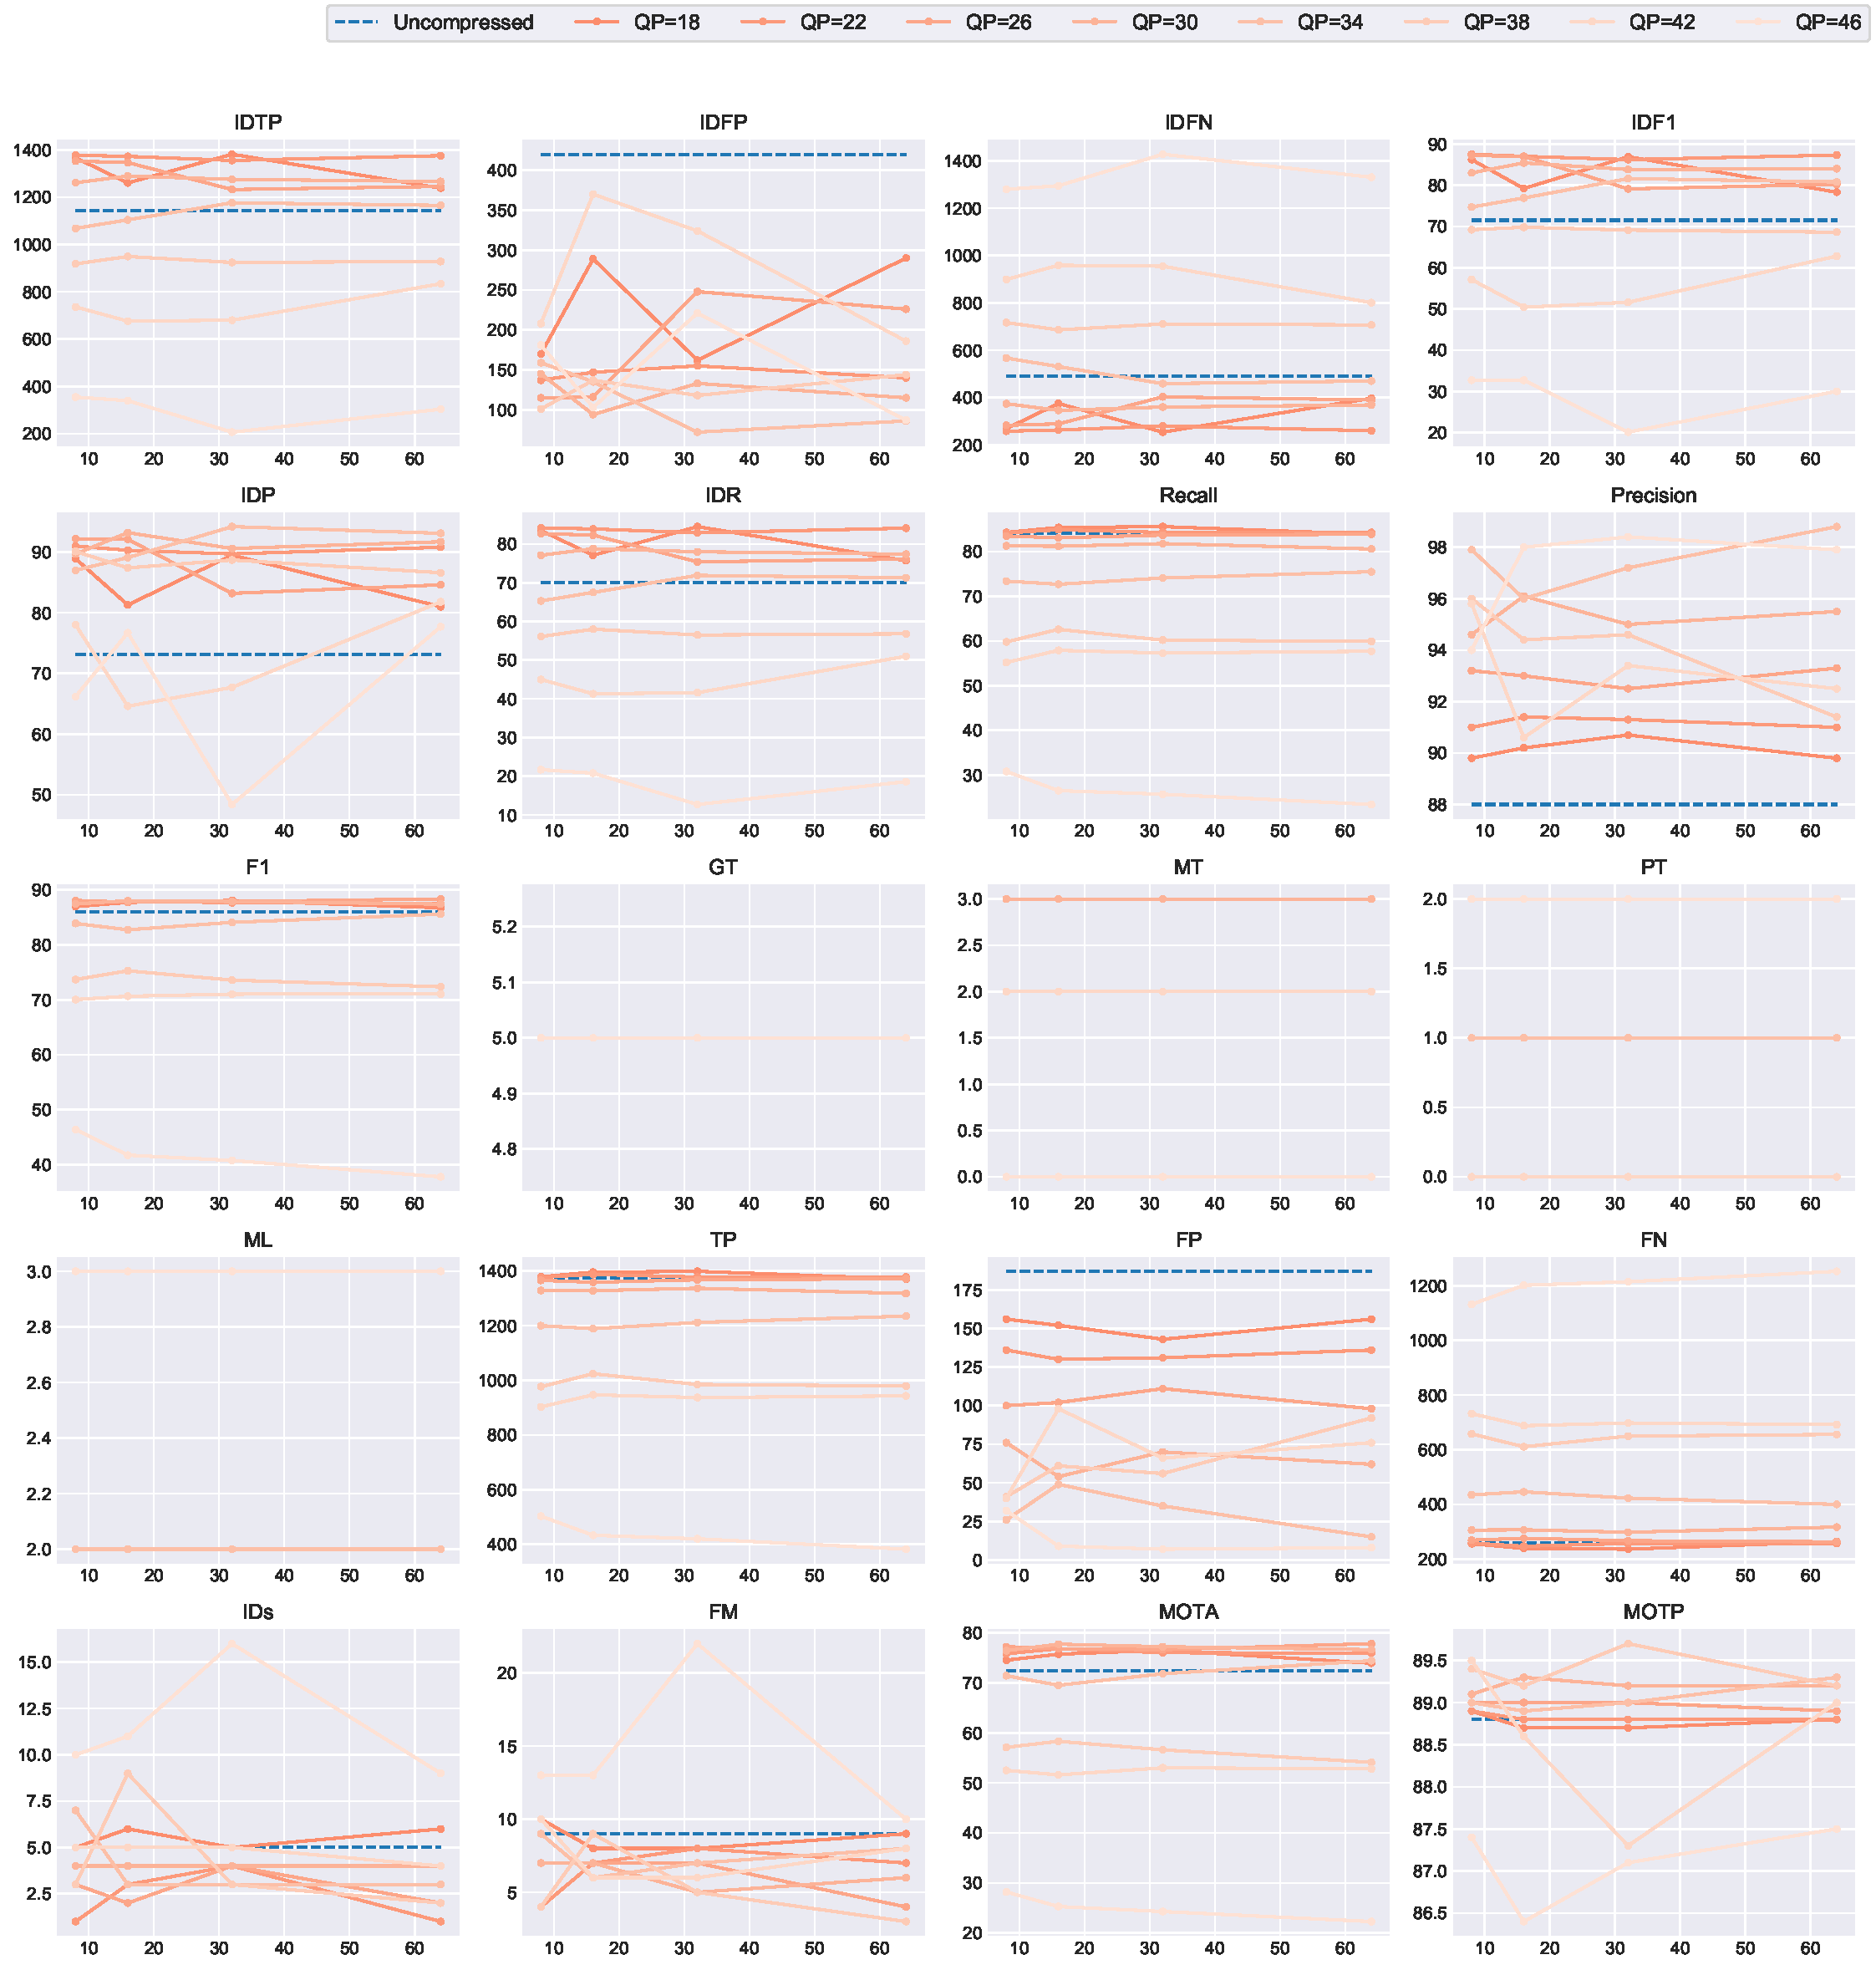
\includegraphics[width=1.0\linewidth]{img/appendix/BlowingBubbles_all_multiplots_msr.pdf}
\caption[Visualization of performance results in Class D BlowingBubbles at different MSR]
{Visualization of performance results in Class D BlowingBubbles at different MSR.}
\label{fig:BlowingBubbles_all_msr}
\end{figure}



% table
\begin{table}
\centering
\caption[Performance results in Class D BlowingBubbles]
{Performance results in Class D BlowingBubbles.}


% table for uncompressed
\begin{subtable}[t]{\linewidth}
\centering
\vspace{0pt}
\resizebox{1.0\linewidth}{!}{
\begin{tabular}{llrrrrrrrrrrrrrrrrrrrr}
\toprule
          QP &          MSR &    IDTP &   IDFP &   IDFN &  IDF1 &   IDP &   IDR &  Recall &  Precision &    F1 &  GT &  MT &  PT &  ML &   TP &  FP &  FN &  IDs &  FM &  MOTA &  MOTP \\
\midrule
Uncompressed & Uncompressed & 1144.00 & 420.00 & 491.00 & 71.50 & 73.10 & 70.00 &   84.20 &      88.00 & 86.06 &   5 &   3 &   0 &   2 & 1376 & 187 & 259 &    5 &   9 & 72.40 & 88.80 \\
\bottomrule
\end{tabular}

}
\caption{Uncompressed Sequence}
\end{subtable}


% table for msr=8
\begin{subtable}[t]{\linewidth}
\centering
\resizebox{1.0\linewidth}{!}{
\begin{tabular}{rrrrrrrrrrrrrrrrrrrrrr}
\toprule
 QP &  MSR &    IDTP &   IDFP &    IDFN &  IDF1 &   IDP &   IDR &  Recall &  Precision &    F1 &  GT &  MT &  PT &  ML &   TP &  FP &   FN &  IDs &  FM &  MOTA &  MOTP \\
\midrule
 18 &    8 & 1366.00 & 170.00 &  269.00 & 86.20 & 88.90 & 83.50 &   84.30 &      89.80 & 86.96 &   5 &   3 &   0 &   2 & 1379 & 156 &  256 &    5 &  10 & 74.50 & 88.90 \\
 22 &    8 & 1377.00 & 137.00 &  258.00 & 87.50 & 91.00 & 84.20 &   84.20 &      91.00 & 87.47 &   5 &   3 &   0 &   2 & 1377 & 136 &  258 &    1 &   4 & 75.80 & 88.90 \\
 26 &    8 & 1352.00 & 115.00 &  283.00 & 87.20 & 92.20 & 82.70 &   83.50 &      93.20 & 88.08 &   5 &   3 &   0 &   2 & 1366 & 100 &  269 &    3 &   7 & 77.20 & 89.00 \\
 30 &    8 & 1261.00 & 145.00 &  374.00 & 83.00 & 89.70 & 77.10 &   81.30 &      94.60 & 87.45 &   5 &   3 &   0 &   2 & 1329 &  76 &  306 &    4 &   7 & 76.40 & 89.10 \\
 34 &    8 & 1068.00 & 159.00 &  567.00 & 74.70 & 87.00 & 65.30 &   73.40 &      97.90 & 83.90 &   5 &   2 &   1 &   2 & 1200 &  26 &  435 &    7 &   9 & 71.40 & 89.00 \\
 38 &    8 &  918.00 & 101.00 &  717.00 & 69.20 & 90.10 & 56.10 &   59.80 &      96.00 & 73.69 &   5 &   2 &   0 &   3 &  977 &  41 &  658 &    3 &   4 & 57.10 & 89.40 \\
 42 &    8 &  736.00 & 208.00 &  899.00 & 57.10 & 78.00 & 45.00 &   55.20 &      95.80 & 70.04 &   5 &   2 &   0 &   3 &  903 &  40 &  732 &    5 &  10 & 52.50 & 89.50 \\
 46 &    8 &  355.00 & 181.00 & 1280.00 & 32.70 & 66.20 & 21.70 &   30.80 &      94.00 & 46.40 &   5 &   0 &   2 &   3 &  503 &  32 & 1132 &   10 &  13 & 28.20 & 87.40 \\
\bottomrule
\end{tabular}

}
\caption{MSR = 8}
\end{subtable}



% table for msr=16
\begin{subtable}[t]{\linewidth}
\centering
\resizebox{1.0\linewidth}{!}{
\begin{tabular}{rrrrrrrrrrrrrrrrrrrrrr}
\toprule
 QP &  MSR &    IDTP &   IDFP &    IDFN &  IDF1 &   IDP &   IDR &  Recall &  Precision &    F1 &  GT &  MT &  PT &  ML &   TP &  FP &   FN &  IDs &  FM &  MOTA &  MOTP \\
\midrule
 18 &   16 & 1260.00 & 289.00 &  375.00 & 79.20 & 81.30 & 77.10 &   85.40 &      90.20 & 87.73 &   5 &   3 &   0 &   2 & 1396 & 152 &  239 &    6 &   8 & 75.70 & 88.70 \\
 22 &   16 & 1372.00 & 147.00 &  263.00 & 87.00 & 90.30 & 83.90 &   84.90 &      91.40 & 88.03 &   5 &   3 &   0 &   2 & 1388 & 130 &  247 &    3 &   7 & 76.80 & 88.80 \\
 26 &   16 & 1346.00 & 116.00 &  289.00 & 87.00 & 92.10 & 82.30 &   83.10 &      93.00 & 87.77 &   5 &   3 &   0 &   2 & 1359 & 102 &  276 &    2 &   7 & 76.80 & 89.00 \\
 30 &   16 & 1289.00 &  94.00 &  346.00 & 85.40 & 93.20 & 78.80 &   81.20 &      96.10 & 88.02 &   5 &   3 &   0 &   2 & 1328 &  54 &  307 &    4 &   7 & 77.70 & 89.30 \\
 34 &   16 & 1104.00 & 135.00 &  531.00 & 76.90 & 89.10 & 67.50 &   72.70 &      96.00 & 82.74 &   5 &   2 &   1 &   2 & 1189 &  49 &  446 &    3 &   6 & 69.50 & 88.90 \\
 38 &   16 &  949.00 & 137.00 &  686.00 & 69.80 & 87.40 & 58.00 &   62.60 &      94.40 & 75.28 &   5 &   2 &   0 &   3 & 1024 &  61 &  611 &    9 &   9 & 58.30 & 89.20 \\
 42 &   16 &  676.00 & 370.00 &  959.00 & 50.40 & 64.60 & 41.30 &   57.90 &      90.60 & 70.65 &   5 &   2 &   0 &   3 &  947 &  98 &  688 &    5 &   6 & 51.60 & 88.60 \\
 46 &   16 &  340.00 & 103.00 & 1295.00 & 32.70 & 76.70 & 20.80 &   26.50 &      98.00 & 41.72 &   5 &   0 &   2 &   3 &  433 &   9 & 1202 &   11 &  13 & 25.30 & 86.40 \\
\bottomrule
\end{tabular}

}
\caption{MSR = 16}
\end{subtable}


% table for msr=32
\begin{subtable}[t]{\linewidth}
\centering
\resizebox{1.0\linewidth}{!}{
\begin{tabular}{rrrrrrrrrrrrrrrrrrrrrr}
\toprule
 QP &  MSR &    IDTP &   IDFP &    IDFN &  IDF1 &   IDP &   IDR &  Recall &  Precision &    F1 &  GT &  MT &  PT &  ML &   TP &  FP &   FN &  IDs &  FM &  MOTA &  MOTP \\
\midrule
 18 &   32 & 1381.00 & 162.00 &  254.00 & 86.90 & 89.50 & 84.50 &   85.60 &      90.70 & 88.08 &   5 &   3 &   0 &   2 & 1399 & 143 &  236 &    5 &   8 & 76.50 & 88.70 \\
 22 &   32 & 1355.00 & 155.00 &  280.00 & 86.20 & 89.70 & 82.90 &   84.30 &      91.30 & 87.66 &   5 &   3 &   0 &   2 & 1378 & 131 &  257 &    4 &   8 & 76.00 & 88.80 \\
 26 &   32 & 1232.00 & 248.00 &  403.00 & 79.10 & 83.20 & 75.40 &   83.70 &      92.50 & 87.88 &   5 &   3 &   0 &   2 & 1368 & 111 &  267 &    4 &   7 & 76.60 & 89.00 \\
 30 &   32 & 1275.00 & 133.00 &  360.00 & 83.80 & 90.60 & 78.00 &   81.80 &      95.00 & 87.91 &   5 &   3 &   0 &   2 & 1337 &  70 &  298 &    4 &   5 & 77.20 & 89.20 \\
 34 &   32 & 1176.00 &  72.00 &  459.00 & 81.60 & 94.20 & 71.90 &   74.10 &      97.20 & 84.09 &   5 &   2 &   1 &   2 & 1212 &  35 &  423 &    3 &   7 & 71.80 & 89.00 \\
 38 &   32 &  924.00 & 118.00 &  711.00 & 69.10 & 88.70 & 56.50 &   60.20 &      94.60 & 73.58 &   5 &   2 &   0 &   3 &  985 &  56 &  650 &    3 &   5 & 56.60 & 89.70 \\
 42 &   32 &  680.00 & 324.00 &  955.00 & 51.60 & 67.70 & 41.60 &   57.30 &      93.40 & 71.03 &   5 &   2 &   0 &   3 &  937 &  66 &  698 &    5 &   6 & 53.00 & 87.30 \\
 46 &   32 &  207.00 & 221.00 & 1428.00 & 20.10 & 48.40 & 12.70 &   25.70 &      98.40 & 40.76 &   5 &   0 &   2 &   3 &  420 &   7 & 1215 &   16 &  22 & 24.30 & 87.10 \\
\bottomrule
\end{tabular}

}
\caption{MSR = 32}
\end{subtable}


% table for msr=64
\begin{subtable}[t]{\linewidth}
\centering
\resizebox{1.0\linewidth}{!}{
\begin{tabular}{rrrrrrrrrrrrrrrrrrrrrr}
\toprule
 QP &  MSR &    IDTP &   IDFP &    IDFN &  IDF1 &   IDP &   IDR &  Recall &  Precision &    F1 &  GT &  MT &  PT &  ML &   TP &  FP &   FN &  IDs &  FM &  MOTA &  MOTP \\
\midrule
 18 &   64 & 1238.00 & 290.00 &  397.00 & 78.30 & 81.00 & 75.70 &   83.90 &      89.80 & 86.75 &   5 &   3 &   0 &   2 & 1371 & 156 &  264 &    6 &   9 & 73.90 & 88.80 \\
 22 &   64 & 1375.00 & 140.00 &  260.00 & 87.30 & 90.80 & 84.10 &   84.30 &      91.00 & 87.52 &   5 &   3 &   0 &   2 & 1378 & 136 &  257 &    1 &   7 & 75.90 & 88.80 \\
 26 &   64 & 1245.00 & 226.00 &  390.00 & 80.20 & 84.60 & 76.10 &   83.90 &      93.30 & 88.35 &   5 &   3 &   0 &   2 & 1372 &  98 &  263 &    2 &   4 & 77.80 & 88.90 \\
 30 &   64 & 1266.00 & 115.00 &  369.00 & 84.00 & 91.70 & 77.40 &   80.60 &      95.50 & 87.42 &   5 &   3 &   0 &   2 & 1318 &  62 &  317 &    4 &   6 & 76.60 & 89.20 \\
 34 &   64 & 1165.00 &  86.00 &  470.00 & 80.80 & 93.10 & 71.30 &   75.50 &      98.80 & 85.59 &   5 &   2 &   1 &   2 & 1235 &  15 &  400 &    3 &   8 & 74.40 & 89.30 \\
 38 &   64 &  928.00 & 144.00 &  707.00 & 68.60 & 86.60 & 56.80 &   59.90 &      91.40 & 72.37 &   5 &   2 &   0 &   3 &  979 &  92 &  656 &    2 &   3 & 54.10 & 89.20 \\
 42 &   64 &  834.00 & 186.00 &  801.00 & 62.80 & 81.80 & 51.00 &   57.70 &      92.50 & 71.07 &   5 &   2 &   0 &   3 &  943 &  76 &  692 &    4 &   8 & 52.80 & 89.00 \\
 46 &   64 &  304.00 &  87.00 & 1331.00 & 30.00 & 77.70 & 18.60 &   23.40 &      97.90 & 37.77 &   5 &   0 &   2 &   3 &  382 &   8 & 1253 &    9 &  10 & 22.30 & 87.50 \\
\bottomrule
\end{tabular}

}
\caption{MSR = 64}
\end{subtable}


\label{tab:BlowingBubbles_all}
\end{table}




\begin{table}[!htbp]
\centering
\caption[Multiple linear regression analysis result for Class D BlowingBubbles]
{Multiple linear regression analysis result for Class D BlowingBubbles}
\resizebox{1.0\linewidth}{!}{
\begin{tabular}{lrrrrrrrrrrrrrrrrrrr}
\toprule
{} &    IDTP &  IDFP &    IDFN &   IDF1 &    IDP &    IDR &  Recall &  Precision &     F1 &    MT &    PT &    ML &      TP &     FP &      FN &   IDs &    FM &   MOTA &  MOTP \\
\midrule
coefficient(Intercept) & 2205.81 & 87.31 & -570.81 & 130.85 & 111.59 & 134.93 &  126.84 &      88.00 & 118.65 &  5.11 & -1.05 &  0.95 & 2074.44 & 217.69 & -439.44 & -1.45 &  2.83 & 113.62 & 90.00 \\
coefficient(QP)        &  -36.25 &  2.46 &   36.25 &  -1.86 &  -0.87 &  -2.22 &   -1.80 &       0.19 &  -1.27 & -0.09 &  0.04 &  0.04 &  -29.41 &  -4.37 &   29.41 &  0.22 &  0.17 &  -1.54 & -0.04 \\
coefficient(MSR)       &   -2.29 &  2.89 &    2.29 &  -0.14 &  -0.24 &  -0.14 &    0.04 &      -0.00 &   0.07 & -0.00 &  0.00 & -0.00 &    0.68 &  -0.07 &   -0.68 &  0.02 &  0.03 &   0.04 & -0.00 \\
coefficient(QP*MSR)    &    0.07 & -0.09 &   -0.07 &   0.00 &   0.01 &   0.00 &   -0.00 &       0.00 &  -0.00 &  0.00 & -0.00 &  0.00 &   -0.03 &   0.00 &    0.03 & -0.00 & -0.00 &  -0.00 &  0.00 \\
p-value(Intercept)     &    0.00 &  0.29 &    0.00 &   0.00 &   0.00 &   0.00 &    0.00 &       0.00 &   0.00 &  0.00 &  0.12 &  0.00 &    0.00 &   0.00 &    0.01 &  0.65 &  0.46 &   0.00 &  0.00 \\
p-value(QP)            &    0.00 &  0.32 &    0.00 &   0.00 &   0.01 &   0.00 &    0.00 &       0.02 &   0.00 &  0.00 &  0.03 &  0.00 &    0.00 &   0.00 &    0.00 &  0.03 &  0.13 &   0.00 &  0.10 \\
p-value(MSR)           &    0.65 &  0.20 &    0.65 &   0.67 &   0.37 &   0.64 &    0.88 &       0.94 &   0.82 &  1.00 &  1.00 &  1.00 &    0.88 &   0.93 &    0.88 &  0.78 &  0.78 &   0.88 &  0.83 \\
p-value(QP*MSR)        &    0.65 &  0.18 &    0.65 &   0.67 &   0.33 &   0.65 &    0.85 &       0.97 &   0.77 &  1.00 &  1.00 &  1.00 &    0.85 &   0.89 &    0.85 &  0.60 &  0.63 &   0.85 &  0.80 \\
\bottomrule
\end{tabular}

}
\label{tab:BlowingBubbles_all_reg}
\end{table}



\newpage

\section{Class D RaceHorsesD}
\label{sec:appendix/RaceHorsesD_all}


% visualization figure
\begin{figure}[!htbp]
\centering
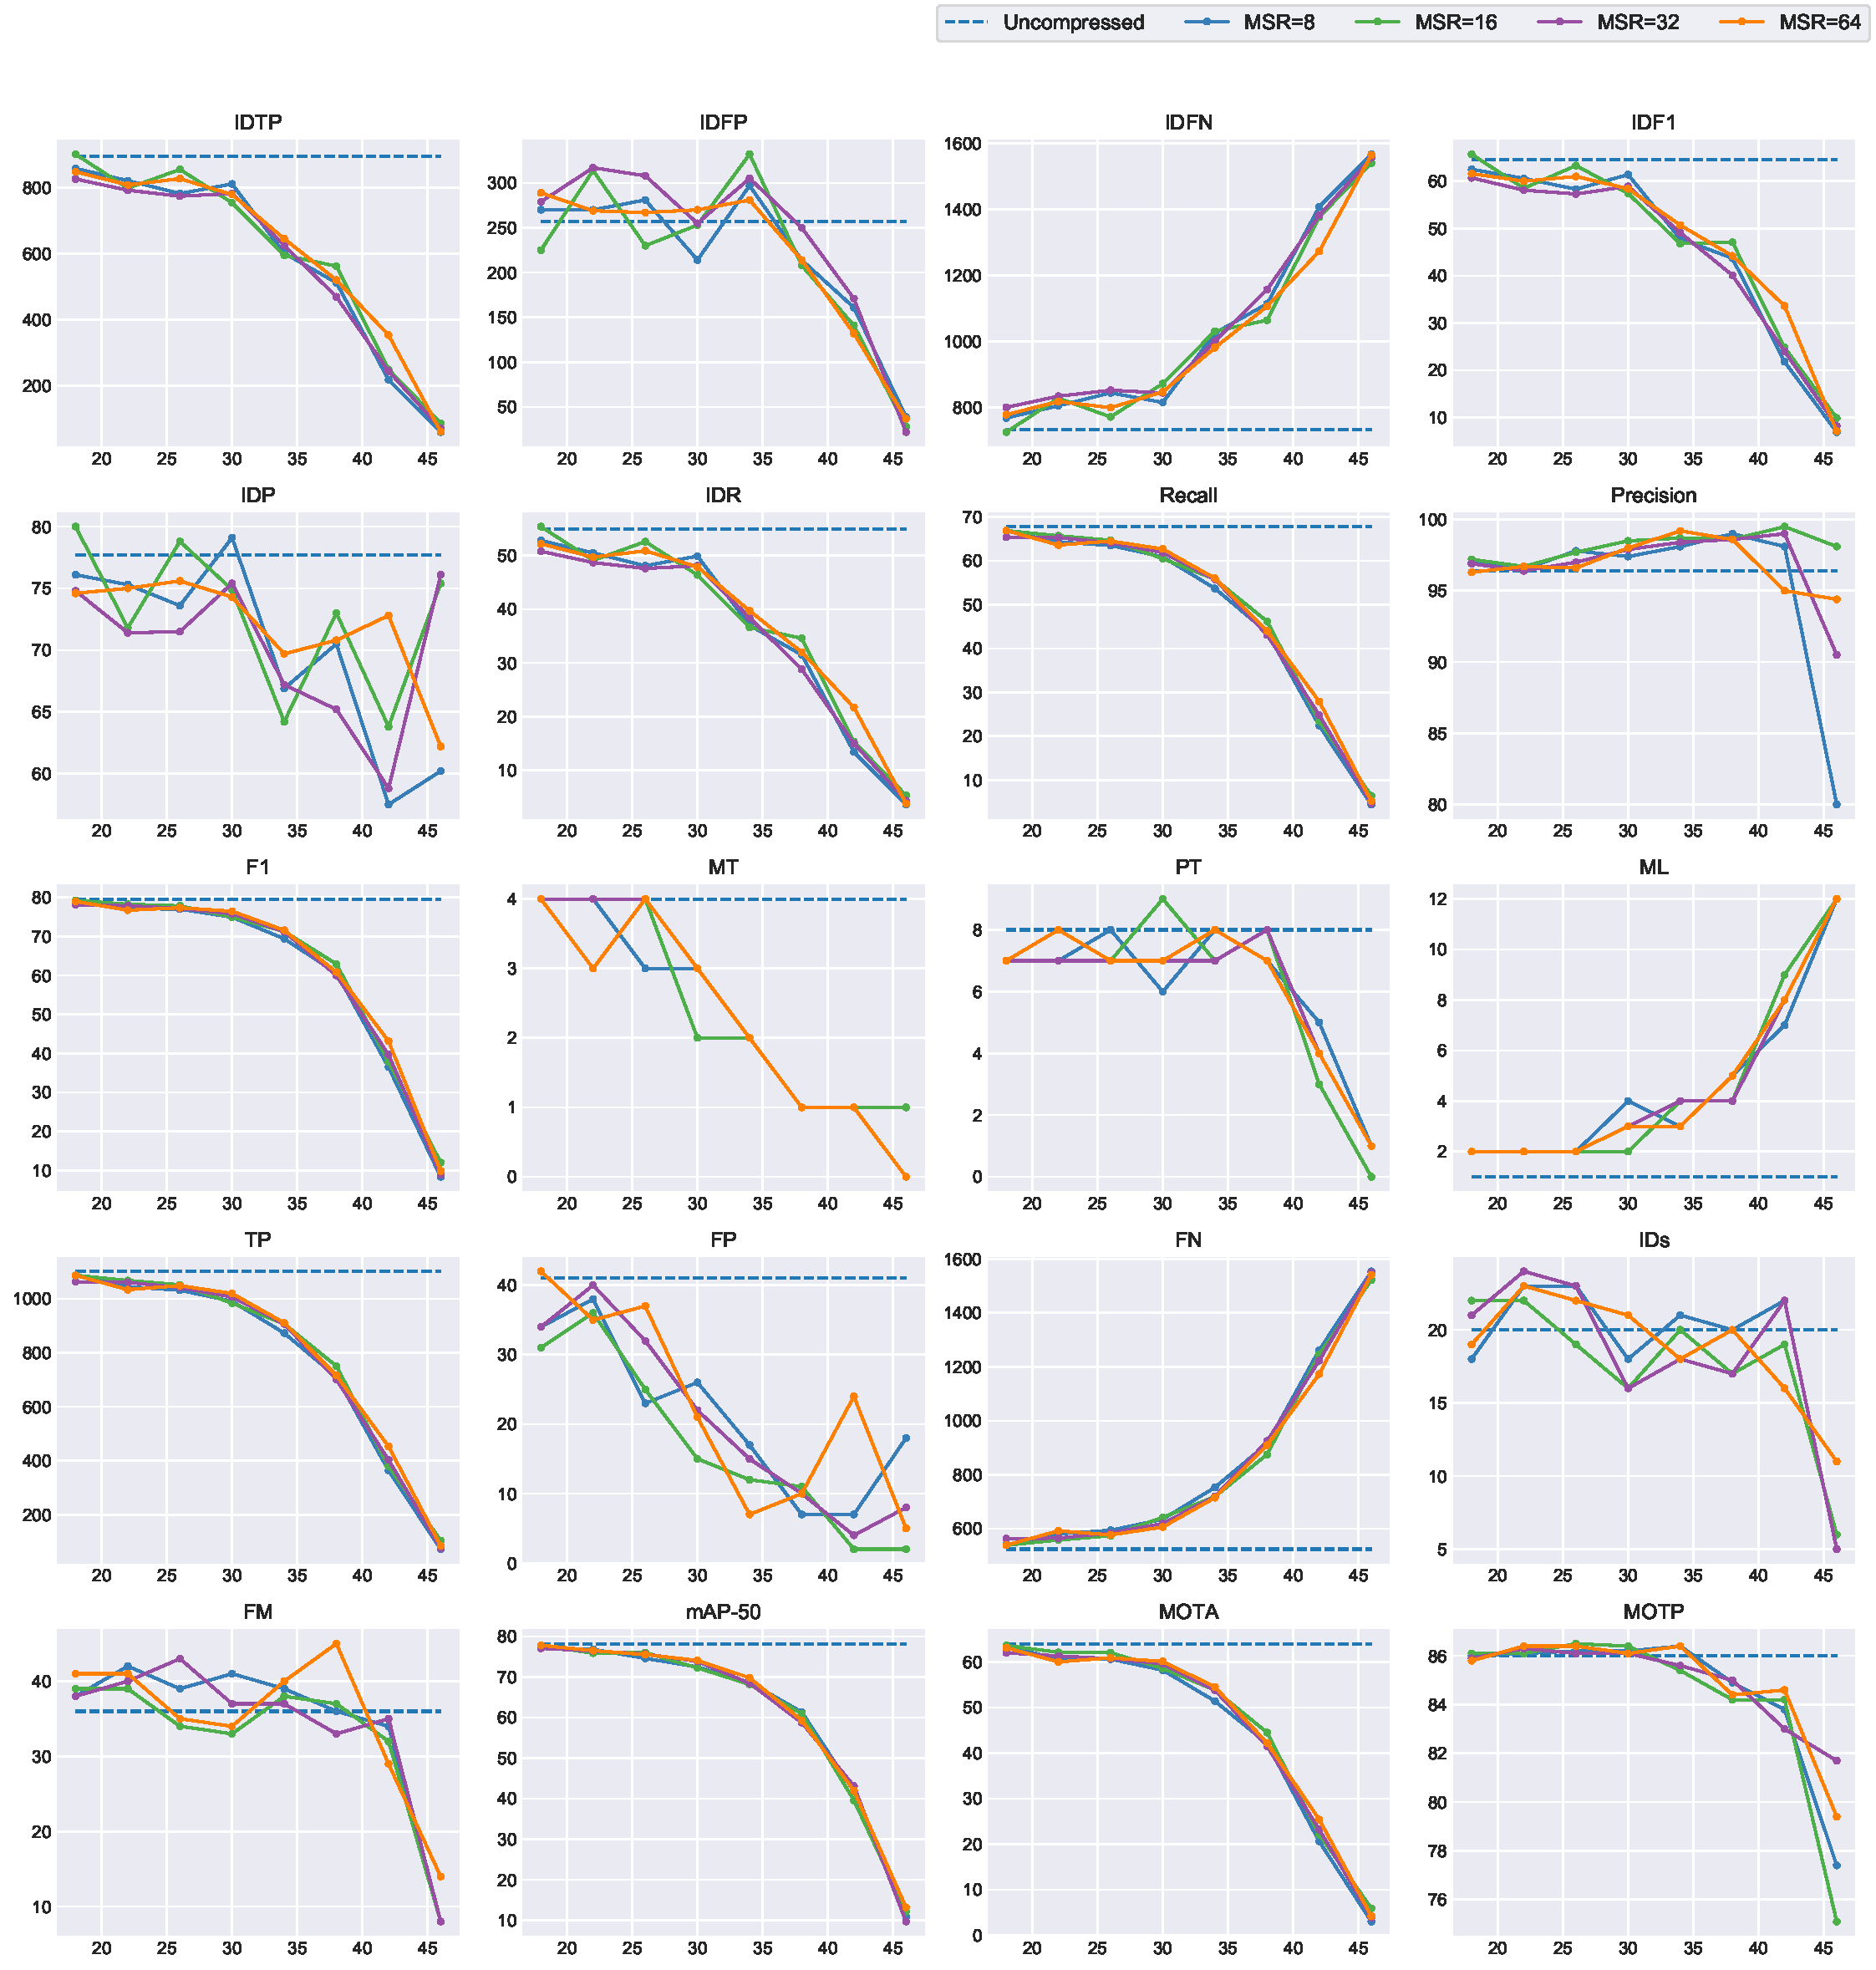
\includegraphics[width=1.0\linewidth]{img/appendix/RaceHorsesD_all_multiplots_qp.pdf}
\caption[Visualization of performance results in Class D RaceHorsesD at different QP]
{Visualization of performance results in Class D RaceHorsesD at different QP.}
\label{fig:RaceHorsesD_all_qp}
\end{figure}

\begin{figure}[!htbp]
\centering
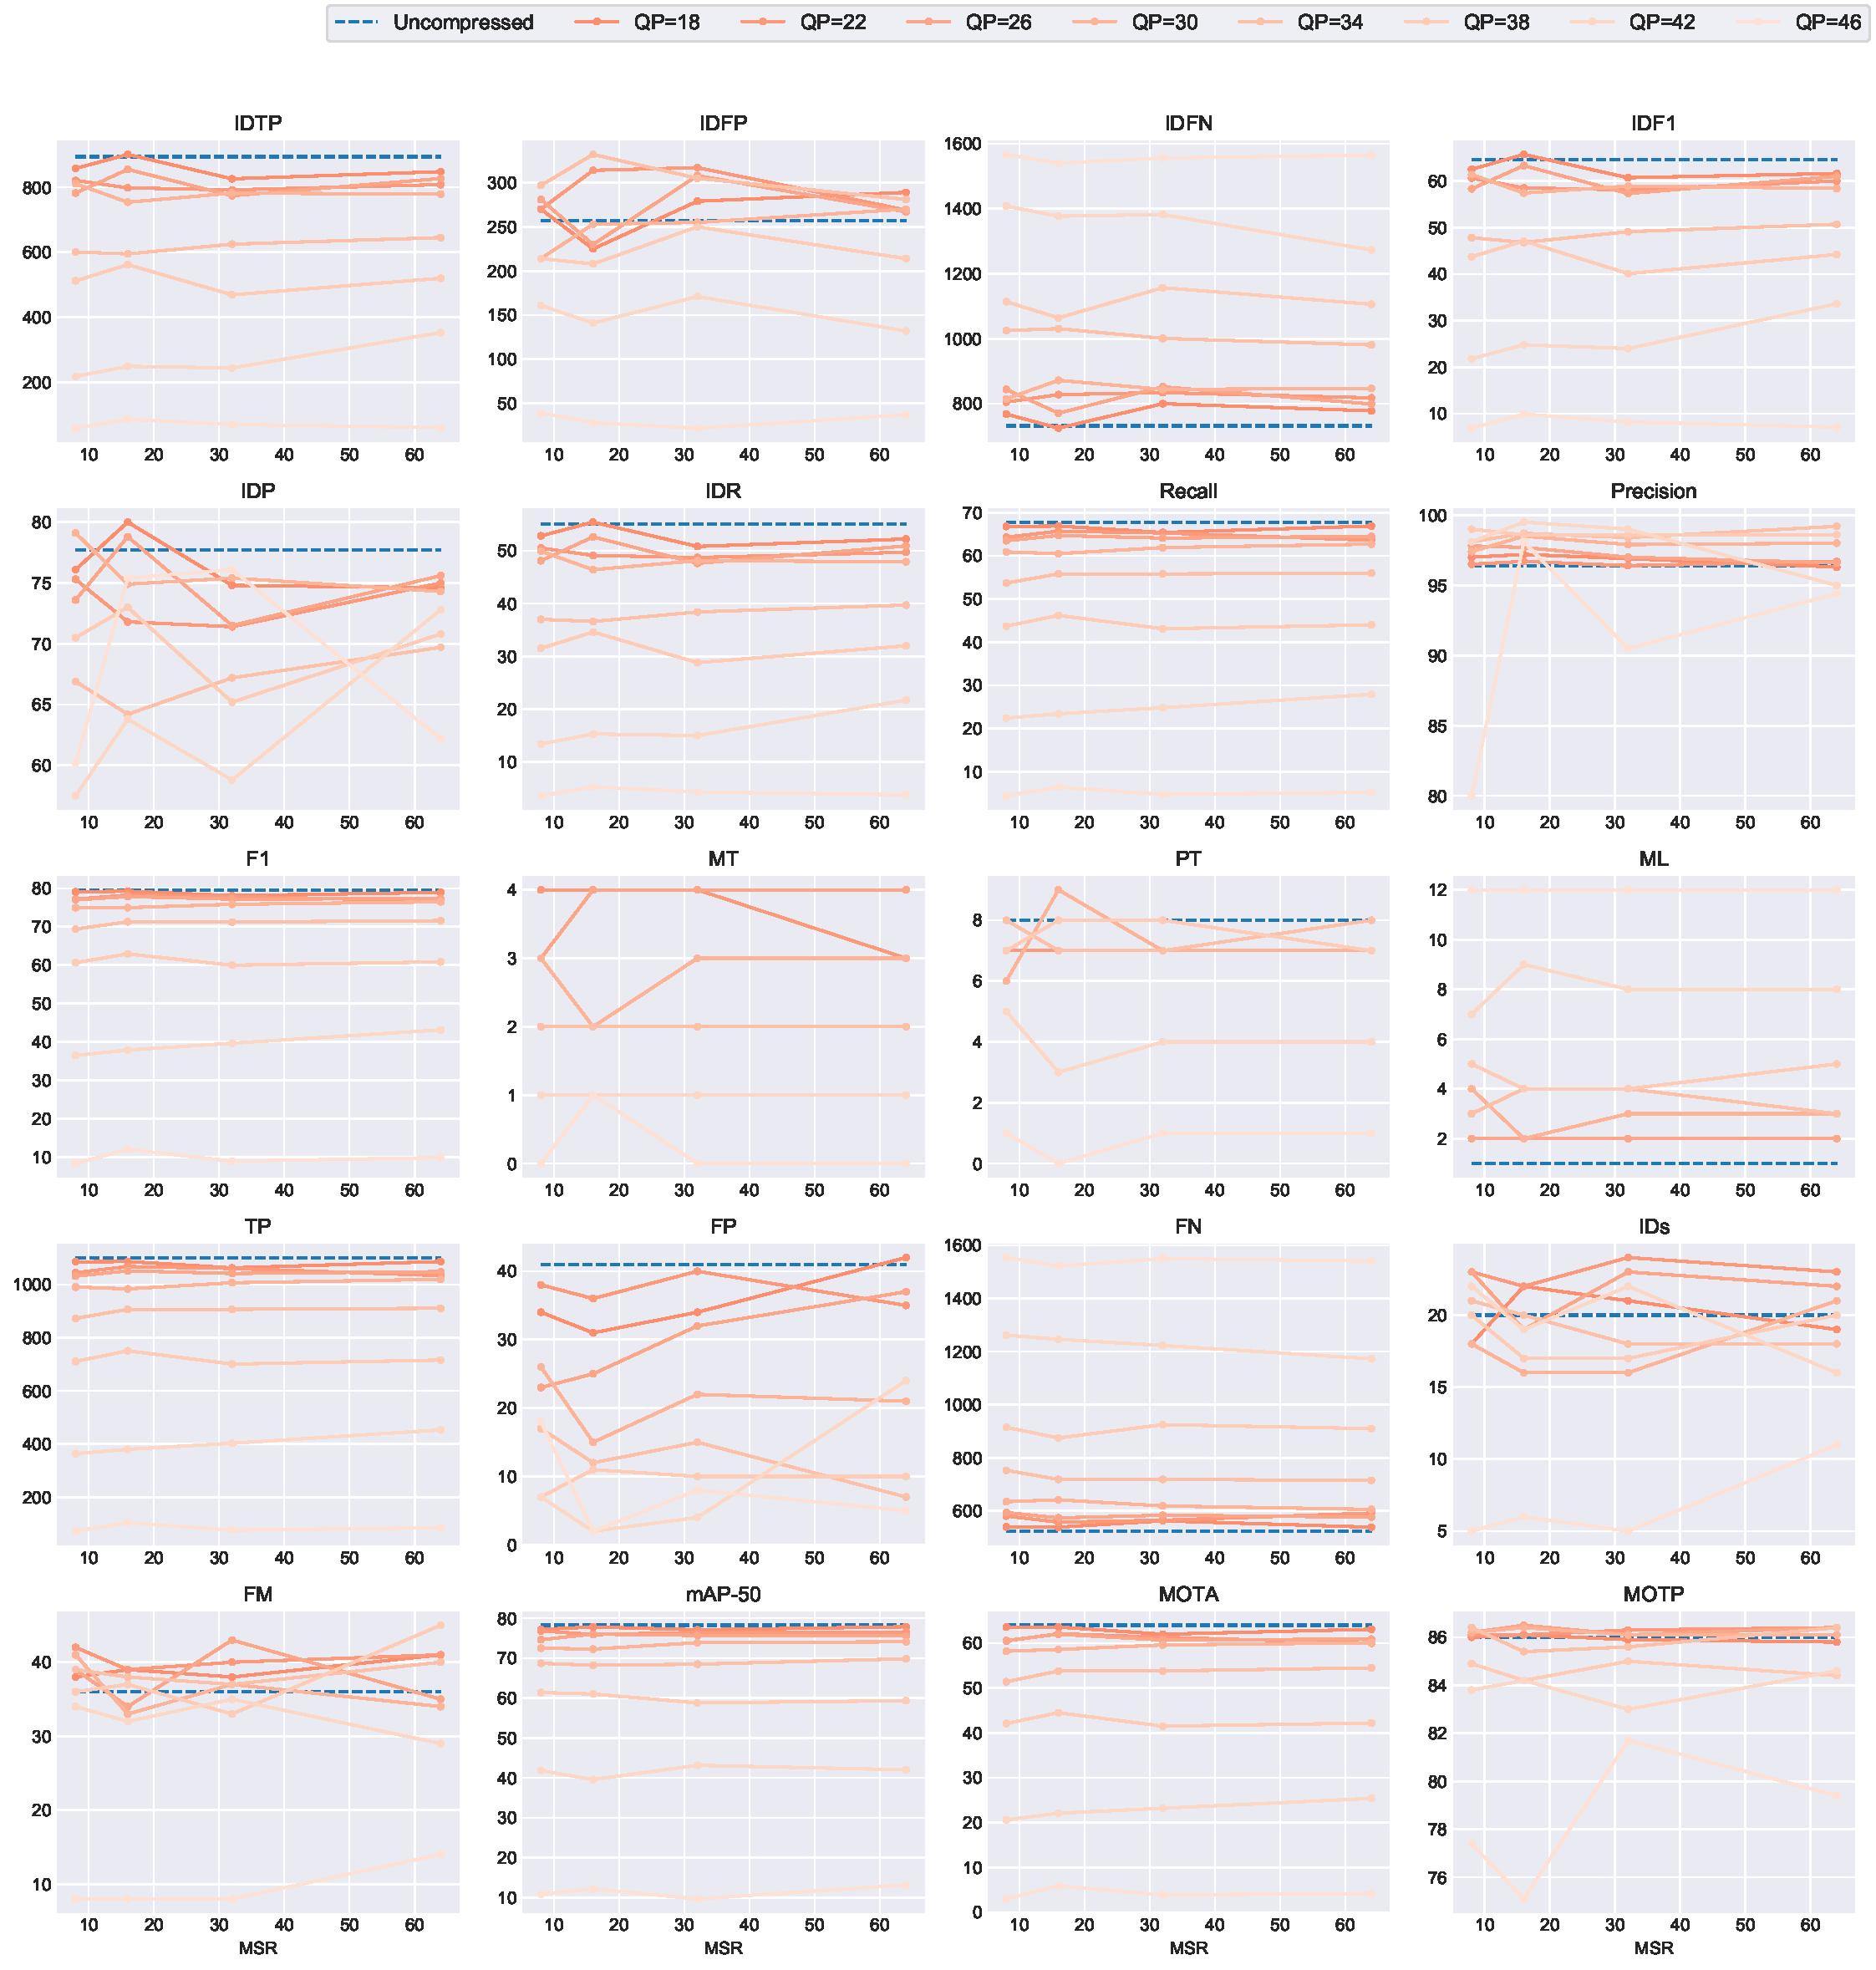
\includegraphics[width=1.0\linewidth]{img/appendix/RaceHorsesD_all_multiplots_msr.pdf}
\caption[Visualization of performance results in Class D RaceHorsesD at different MSR]
{Visualization of performance results in Class D RaceHorsesD at different MSR.}
\label{fig:RaceHorsesD_all_msr}
\end{figure}



% table
\begin{table}
\centering
\caption[Performance results in Class D RaceHorsesD]
{Performance results in Class D RaceHorsesD.}


% table for uncompressed
\begin{subtable}[t]{\linewidth}
\centering
\vspace{0pt}
\resizebox{1.0\linewidth}{!}{
\begin{tabular}{llrrrrrrrrrrrrrrrrrrrr}
\toprule
          QP &          MSR &   IDTP &   IDFP &   IDFN &  IDF1 &   IDP &   IDR &  Recall &  Precision &    F1 &  GT &  MT &  PT &  ML &   TP &  FP &  FN &  IDs &  FM &  MOTA &  MOTP \\
\midrule
Uncompressed & Uncompressed & 894.00 & 257.00 & 732.00 & 64.60 & 77.70 & 55.00 &   67.80 &      96.40 & 79.61 &  13 &   4 &   8 &   1 & 1102 &  41 & 524 &   20 &  36 & 64.00 & 86.00 \\
\bottomrule
\end{tabular}

}
\caption{Uncompressed Sequence}
\end{subtable}


% table for msr=8
\begin{subtable}[t]{\linewidth}
\centering
\resizebox{1.0\linewidth}{!}{
\begin{tabular}{rrrrrrrrrrrrrrrrrrrrrr}
\toprule
 QP &  MSR &   IDTP &   IDFP &    IDFN &  IDF1 &   IDP &   IDR &  Recall &  Precision &    F1 &  GT &  MT &  PT &  ML &   TP &  FP &   FN &  IDs &  FM &  MOTA &  MOTP \\
\midrule
 18 &    8 & 858.00 & 270.00 &  768.00 & 62.50 & 76.10 & 52.80 &   66.80 &      97.00 & 79.12 &  13 &   4 &   7 &   2 & 1086 &  34 &  540 &   18 &  38 & 63.60 & 86.00 \\
 22 &    8 & 821.00 & 270.00 &  805.00 & 60.60 & 75.30 & 50.50 &   64.30 &      96.50 & 77.18 &  13 &   4 &   7 &   2 & 1045 &  38 &  581 &   23 &  42 & 60.50 & 86.10 \\
 26 &    8 & 782.00 & 281.00 &  844.00 & 58.30 & 73.60 & 48.10 &   63.50 &      97.80 & 77.00 &  13 &   3 &   8 &   2 & 1032 &  23 &  594 &   23 &  39 & 60.60 & 86.20 \\
 30 &    8 & 811.00 & 214.00 &  815.00 & 61.40 & 79.10 & 49.90 &   60.90 &      97.40 & 74.94 &  13 &   3 &   6 &   4 &  991 &  26 &  635 &   18 &  41 & 58.20 & 86.20 \\
 34 &    8 & 601.00 & 297.00 & 1025.00 & 47.80 & 66.90 & 37.00 &   53.70 &      98.10 & 69.41 &  13 &   2 &   8 &   3 &  873 &  17 &  753 &   21 &  39 & 51.40 & 86.40 \\
 38 &    8 & 512.00 & 214.00 & 1114.00 & 43.70 & 70.50 & 31.50 &   43.70 &      99.00 & 60.63 &  13 &   1 &   7 &   5 &  711 &   7 &  915 &   20 &  36 & 42.10 & 84.90 \\
 42 &    8 & 218.00 & 161.00 & 1408.00 & 21.80 & 57.50 & 13.40 &   22.40 &      98.10 & 36.47 &  13 &   1 &   5 &   7 &  364 &   7 & 1262 &   22 &  34 & 20.60 & 83.80 \\
 46 &    8 &  59.00 &  39.00 & 1567.00 &  6.90 & 60.20 &  3.60 &    4.40 &      80.00 &  8.34 &  13 &   0 &   1 &  12 &   72 &  18 & 1554 &    5 &   8 &  3.00 & 77.40 \\
\bottomrule
\end{tabular}

}
\caption{MSR = 8}
\end{subtable}



% table for msr=16
\begin{subtable}[t]{\linewidth}
\centering
\resizebox{1.0\linewidth}{!}{
\begin{tabular}{rrrrrrrrrrrrrrrrrrrrrr}
\toprule
 QP &  MSR &   IDTP &   IDFP &    IDFN &  IDF1 &   IDP &   IDR &  Recall &  Precision &    F1 &  GT &  MT &  PT &  ML &   TP &  FP &   FN &  IDs &  FM &  MOTA &  MOTP \\
\midrule
 18 &   16 & 901.00 & 225.00 &  725.00 & 65.70 & 80.00 & 55.40 &   66.90 &      97.20 & 79.25 &  13 &   4 &   7 &   2 & 1087 &  31 &  539 &   22 &  39 & 63.60 & 86.10 \\
 22 &   16 & 798.00 & 314.00 &  828.00 & 58.50 & 71.80 & 49.10 &   65.70 &      96.70 & 78.24 &  13 &   4 &   7 &   2 & 1068 &  36 &  558 &   22 &  39 & 62.10 & 86.10 \\
 26 &   16 & 855.00 & 230.00 &  771.00 & 63.30 & 78.80 & 52.60 &   64.70 &      97.70 & 77.85 &  13 &   4 &   7 &   2 & 1052 &  25 &  574 &   19 &  34 & 62.00 & 86.50 \\
 30 &   16 & 754.00 & 253.00 &  872.00 & 57.40 & 74.90 & 46.40 &   60.50 &      98.50 & 74.96 &  13 &   2 &   9 &   2 &  984 &  15 &  642 &   16 &  33 & 58.60 & 86.40 \\
 34 &   16 & 595.00 & 332.00 & 1031.00 & 46.80 & 64.20 & 36.60 &   55.80 &      98.70 & 71.29 &  13 &   2 &   7 &   4 &  907 &  12 &  719 &   20 &  38 & 53.80 & 85.40 \\
 38 &   16 & 562.00 & 208.00 & 1064.00 & 47.10 & 73.00 & 34.60 &   46.20 &      98.60 & 62.92 &  13 &   1 &   8 &   4 &  751 &  11 &  875 &   17 &  37 & 44.50 & 84.20 \\
 42 &   16 & 249.00 & 141.00 & 1377.00 & 24.80 & 63.80 & 15.30 &   23.40 &      99.50 & 37.89 &  13 &   1 &   3 &   9 &  380 &   2 & 1246 &   19 &  32 & 22.10 & 84.20 \\
 46 &   16 &  86.00 &  28.00 & 1540.00 &  9.90 & 75.40 &  5.30 &    6.40 &      98.10 & 12.02 &  13 &   1 &   0 &  12 &  104 &   2 & 1522 &    6 &   8 &  5.90 & 75.10 \\
\bottomrule
\end{tabular}

}
\caption{MSR = 16}
\end{subtable}


% table for msr=32
\begin{subtable}[t]{\linewidth}
\centering
\resizebox{1.0\linewidth}{!}{
\begin{tabular}{rrrrrrrrrrrrrrrrrrrrrr}
\toprule
 QP &  MSR &   IDTP &   IDFP &    IDFN &  IDF1 &   IDP &   IDR &  Recall &  Precision &    F1 &  GT &  MT &  PT &  ML &   TP &  FP &   FN &  IDs &  FM &  MOTA &  MOTP \\
\midrule
 18 &   32 & 826.00 & 279.00 &  800.00 & 60.70 & 74.80 & 50.80 &   65.40 &      96.90 & 78.09 &  13 &   4 &   7 &   2 & 1063 &  34 &  563 &   21 &  38 & 62.00 & 85.90 \\
 22 &   32 & 792.00 & 317.00 &  834.00 & 58.10 & 71.40 & 48.70 &   65.30 &      96.40 & 77.86 &  13 &   4 &   7 &   2 & 1061 &  40 &  565 &   24 &  40 & 61.30 & 86.30 \\
 26 &   32 & 774.00 & 308.00 &  852.00 & 57.30 & 71.50 & 47.60 &   64.10 &      97.00 & 77.19 &  13 &   4 &   7 &   2 & 1042 &  32 &  584 &   23 &  43 & 60.70 & 86.10 \\
 30 &   32 & 782.00 & 255.00 &  844.00 & 58.90 & 75.40 & 48.10 &   61.90 &      97.90 & 75.84 &  13 &   3 &   7 &   3 & 1007 &  22 &  619 &   16 &  37 & 59.60 & 86.10 \\
 34 &   32 & 625.00 & 305.00 & 1001.00 & 49.10 & 67.20 & 38.40 &   55.80 &      98.40 & 71.22 &  13 &   2 &   7 &   4 &  907 &  15 &  719 &   18 &  37 & 53.80 & 85.60 \\
 38 &   32 & 469.00 & 250.00 & 1157.00 & 40.10 & 65.20 & 28.80 &   43.10 &      98.60 & 59.98 &  13 &   1 &   8 &   4 &  701 &  10 &  925 &   17 &  33 & 41.50 & 85.00 \\
 42 &   32 & 244.00 & 171.00 & 1382.00 & 24.00 & 58.80 & 15.00 &   24.80 &      99.00 & 39.66 &  13 &   1 &   4 &   8 &  403 &   4 & 1223 &   22 &  35 & 23.20 & 83.00 \\
 46 &   32 &  70.00 &  22.00 & 1556.00 &  8.20 & 76.10 &  4.30 &    4.70 &      90.50 &  8.94 &  13 &   0 &   1 &  12 &   76 &   8 & 1550 &    5 &   8 &  3.90 & 81.70 \\
\bottomrule
\end{tabular}

}
\caption{MSR = 32}
\end{subtable}


% table for msr=64
\begin{subtable}[t]{\linewidth}
\centering
\resizebox{1.0\linewidth}{!}{
\begin{tabular}{rrrrrrrrrrrrrrrrrrrrrr}
\toprule
 QP &  MSR &   IDTP &   IDFP &    IDFN &  IDF1 &   IDP &   IDR &  Recall &  Precision &    F1 &  GT &  MT &  PT &  ML &   TP &  FP &   FN &  IDs &  FM &  MOTA &  MOTP \\
\midrule
 18 &   64 & 848.00 & 289.00 &  778.00 & 61.60 & 74.60 & 52.20 &   66.90 &      96.30 & 78.95 &  13 &   4 &   7 &   2 & 1087 &  42 &  539 &   19 &  41 & 63.10 & 85.80 \\
 22 &   64 & 808.00 & 269.00 &  818.00 & 60.00 & 75.00 & 49.70 &   63.60 &      96.70 & 76.73 &  13 &   3 &   8 &   2 & 1034 &  35 &  592 &   23 &  41 & 60.00 & 86.40 \\
 26 &   64 & 827.00 & 267.00 &  799.00 & 61.00 & 75.60 & 50.90 &   64.50 &      96.60 & 77.35 &  13 &   4 &   7 &   2 & 1049 &  37 &  577 &   22 &  35 & 60.90 & 86.40 \\
 30 &   64 & 779.00 & 270.00 &  847.00 & 58.40 & 74.30 & 47.90 &   62.70 &      98.00 & 76.47 &  13 &   3 &   7 &   3 & 1020 &  21 &  606 &   21 &  34 & 60.10 & 86.10 \\
 34 &   64 & 645.00 & 281.00 &  981.00 & 50.70 & 69.70 & 39.70 &   56.00 &      99.20 & 71.59 &  13 &   2 &   8 &   3 &  911 &   7 &  715 &   18 &  40 & 54.50 & 86.40 \\
 38 &   64 & 520.00 & 214.00 & 1106.00 & 44.20 & 70.80 & 32.00 &   44.00 &      98.60 & 60.85 &  13 &   1 &   7 &   5 &  716 &  10 &  910 &   20 &  45 & 42.20 & 84.40 \\
 42 &   64 & 353.00 & 132.00 & 1273.00 & 33.60 & 72.80 & 21.70 &   27.90 &      95.00 & 43.13 &  13 &   1 &   4 &   8 &  453 &  24 & 1173 &   16 &  29 & 25.40 & 84.60 \\
 46 &   64 &  61.00 &  37.00 & 1565.00 &  7.10 & 62.20 &  3.80 &    5.20 &      94.40 &  9.86 &  13 &   0 &   1 &  12 &   85 &   5 & 1541 &   11 &  14 &  4.20 & 79.40 \\
\bottomrule
\end{tabular}

}
\caption{MSR = 64}
\end{subtable}


\label{tab:RaceHorsesD_all}
\end{table}




\begin{table}[!htbp]
\centering
\caption[Multiple linear regression analysis result for Class D RaceHorsesD]
{Multiple linear regression analysis result for Class D RaceHorsesD}
\resizebox{1.0\linewidth}{!}{
\begin{tabular}{lrrrrrrrrrrrrrrrrrrr}
\toprule
{} &    IDTP &   IDFP &   IDFN &   IDF1 &   IDP &   IDR &  Recall &  Precision &     F1 &    MT &    PT &    ML &      TP &    FP &      FN &   IDs &    FM &   MOTA &  MOTP \\
\midrule
coefficient(Intercept) & 1504.61 & 434.68 & 121.39 & 106.45 & 86.41 & 92.57 &  115.52 &     101.88 & 131.96 &  6.99 & 11.56 & -5.55 & 1877.77 & 53.52 & -251.77 & 29.85 & 58.65 & 110.33 & 92.40 \\
coefficient(QP)        &  -28.83 &  -6.67 &  28.83 &  -1.91 & -0.49 & -1.77 &   -2.12 &      -0.16 &  -2.22 & -0.15 & -0.17 &  0.32 &  -34.41 & -1.09 &   34.41 & -0.37 & -0.79 &  -2.03 & -0.25 \\
coefficient(MSR)       &   -1.07 &   0.70 &   1.07 &  -0.09 & -0.10 & -0.07 &   -0.03 &      -0.07 &  -0.04 & -0.00 &  0.00 & -0.00 &   -0.52 &  0.15 &    0.52 & -0.01 & -0.05 &  -0.04 & -0.04 \\
coefficient(QP*MSR)    &    0.04 &  -0.02 &  -0.04 &   0.00 &  0.00 &  0.00 &    0.00 &       0.00 &   0.00 & -0.00 & -0.00 &  0.00 &    0.03 & -0.00 &   -0.03 &  0.00 &  0.00 &   0.00 &  0.00 \\
p-value(Intercept)     &    0.00 &   0.00 &   0.31 &   0.00 &  0.00 &  0.00 &    0.00 &       0.00 &   0.00 &  0.00 &  0.00 &  0.01 &    0.00 &  0.00 &    0.15 &  0.00 &  0.00 &   0.00 &  0.00 \\
p-value(QP)            &    0.00 &   0.00 &   0.00 &   0.00 &  0.01 &  0.00 &    0.00 &       0.17 &   0.00 &  0.00 &  0.01 &  0.00 &    0.00 &  0.00 &    0.00 &  0.01 &  0.00 &   0.00 &  0.00 \\
p-value(MSR)           &    0.74 &   0.70 &   0.74 &   0.73 &  0.52 &  0.74 &    0.91 &       0.52 &   0.91 &  0.98 &  0.94 &  0.95 &    0.91 &  0.43 &    0.91 &  0.93 &  0.84 &   0.89 &  0.55 \\
p-value(QP*MSR)        &    0.67 &   0.72 &   0.67 &   0.66 &  0.44 &  0.67 &    0.86 &       0.46 &   0.87 &  0.97 &  0.95 &  0.94 &    0.86 &  0.61 &    0.86 &  0.87 &  0.77 &   0.85 &  0.44 \\
\bottomrule
\end{tabular}

}
\label{tab:RaceHorsesD_all_reg}
\end{table}



\newpage

\section{Class E FourPeople}
\label{sec:appendix/FourPeople_all}


% visualization figure
\begin{figure}[!htbp]
\centering
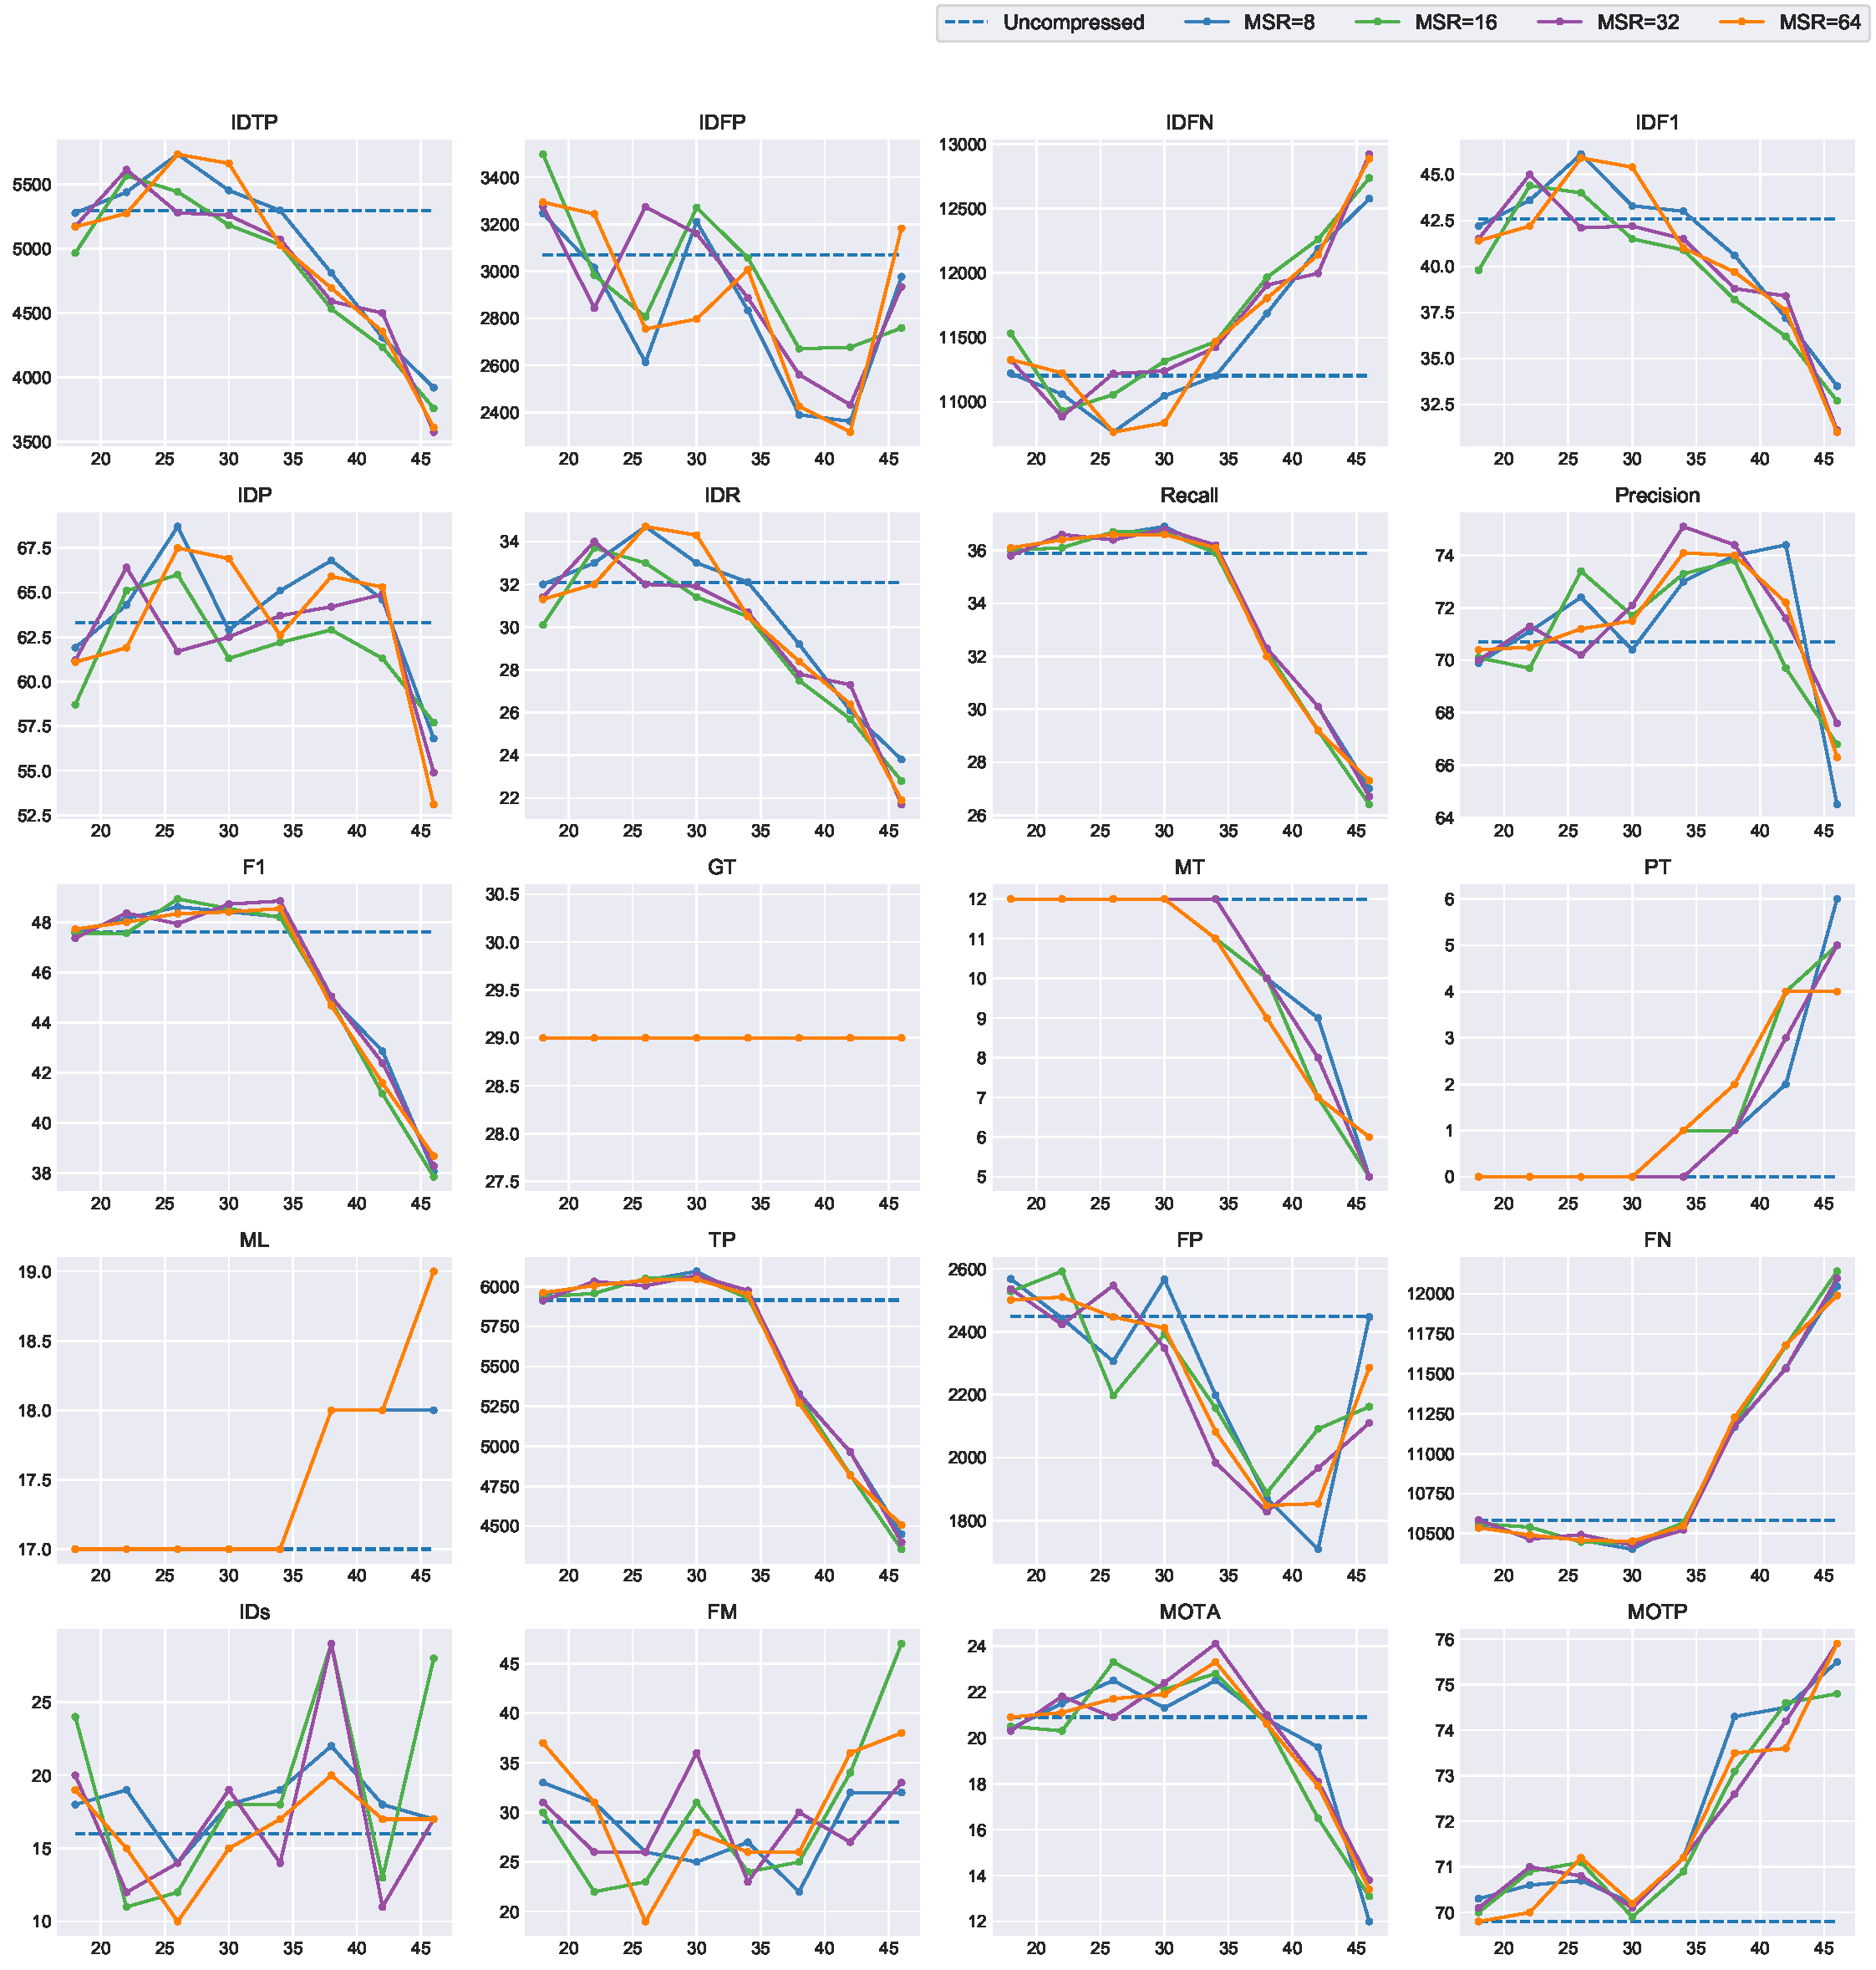
\includegraphics[width=1.0\linewidth]{img/appendix/FourPeople_all_multiplots_qp.pdf}
\caption[Result of all object classes in Class E FourPeople with Horizontal Axis of QP]{}
\label{fig:FourPeople_all_qp}
\end{figure}

\begin{figure}[!htbp]
\centering
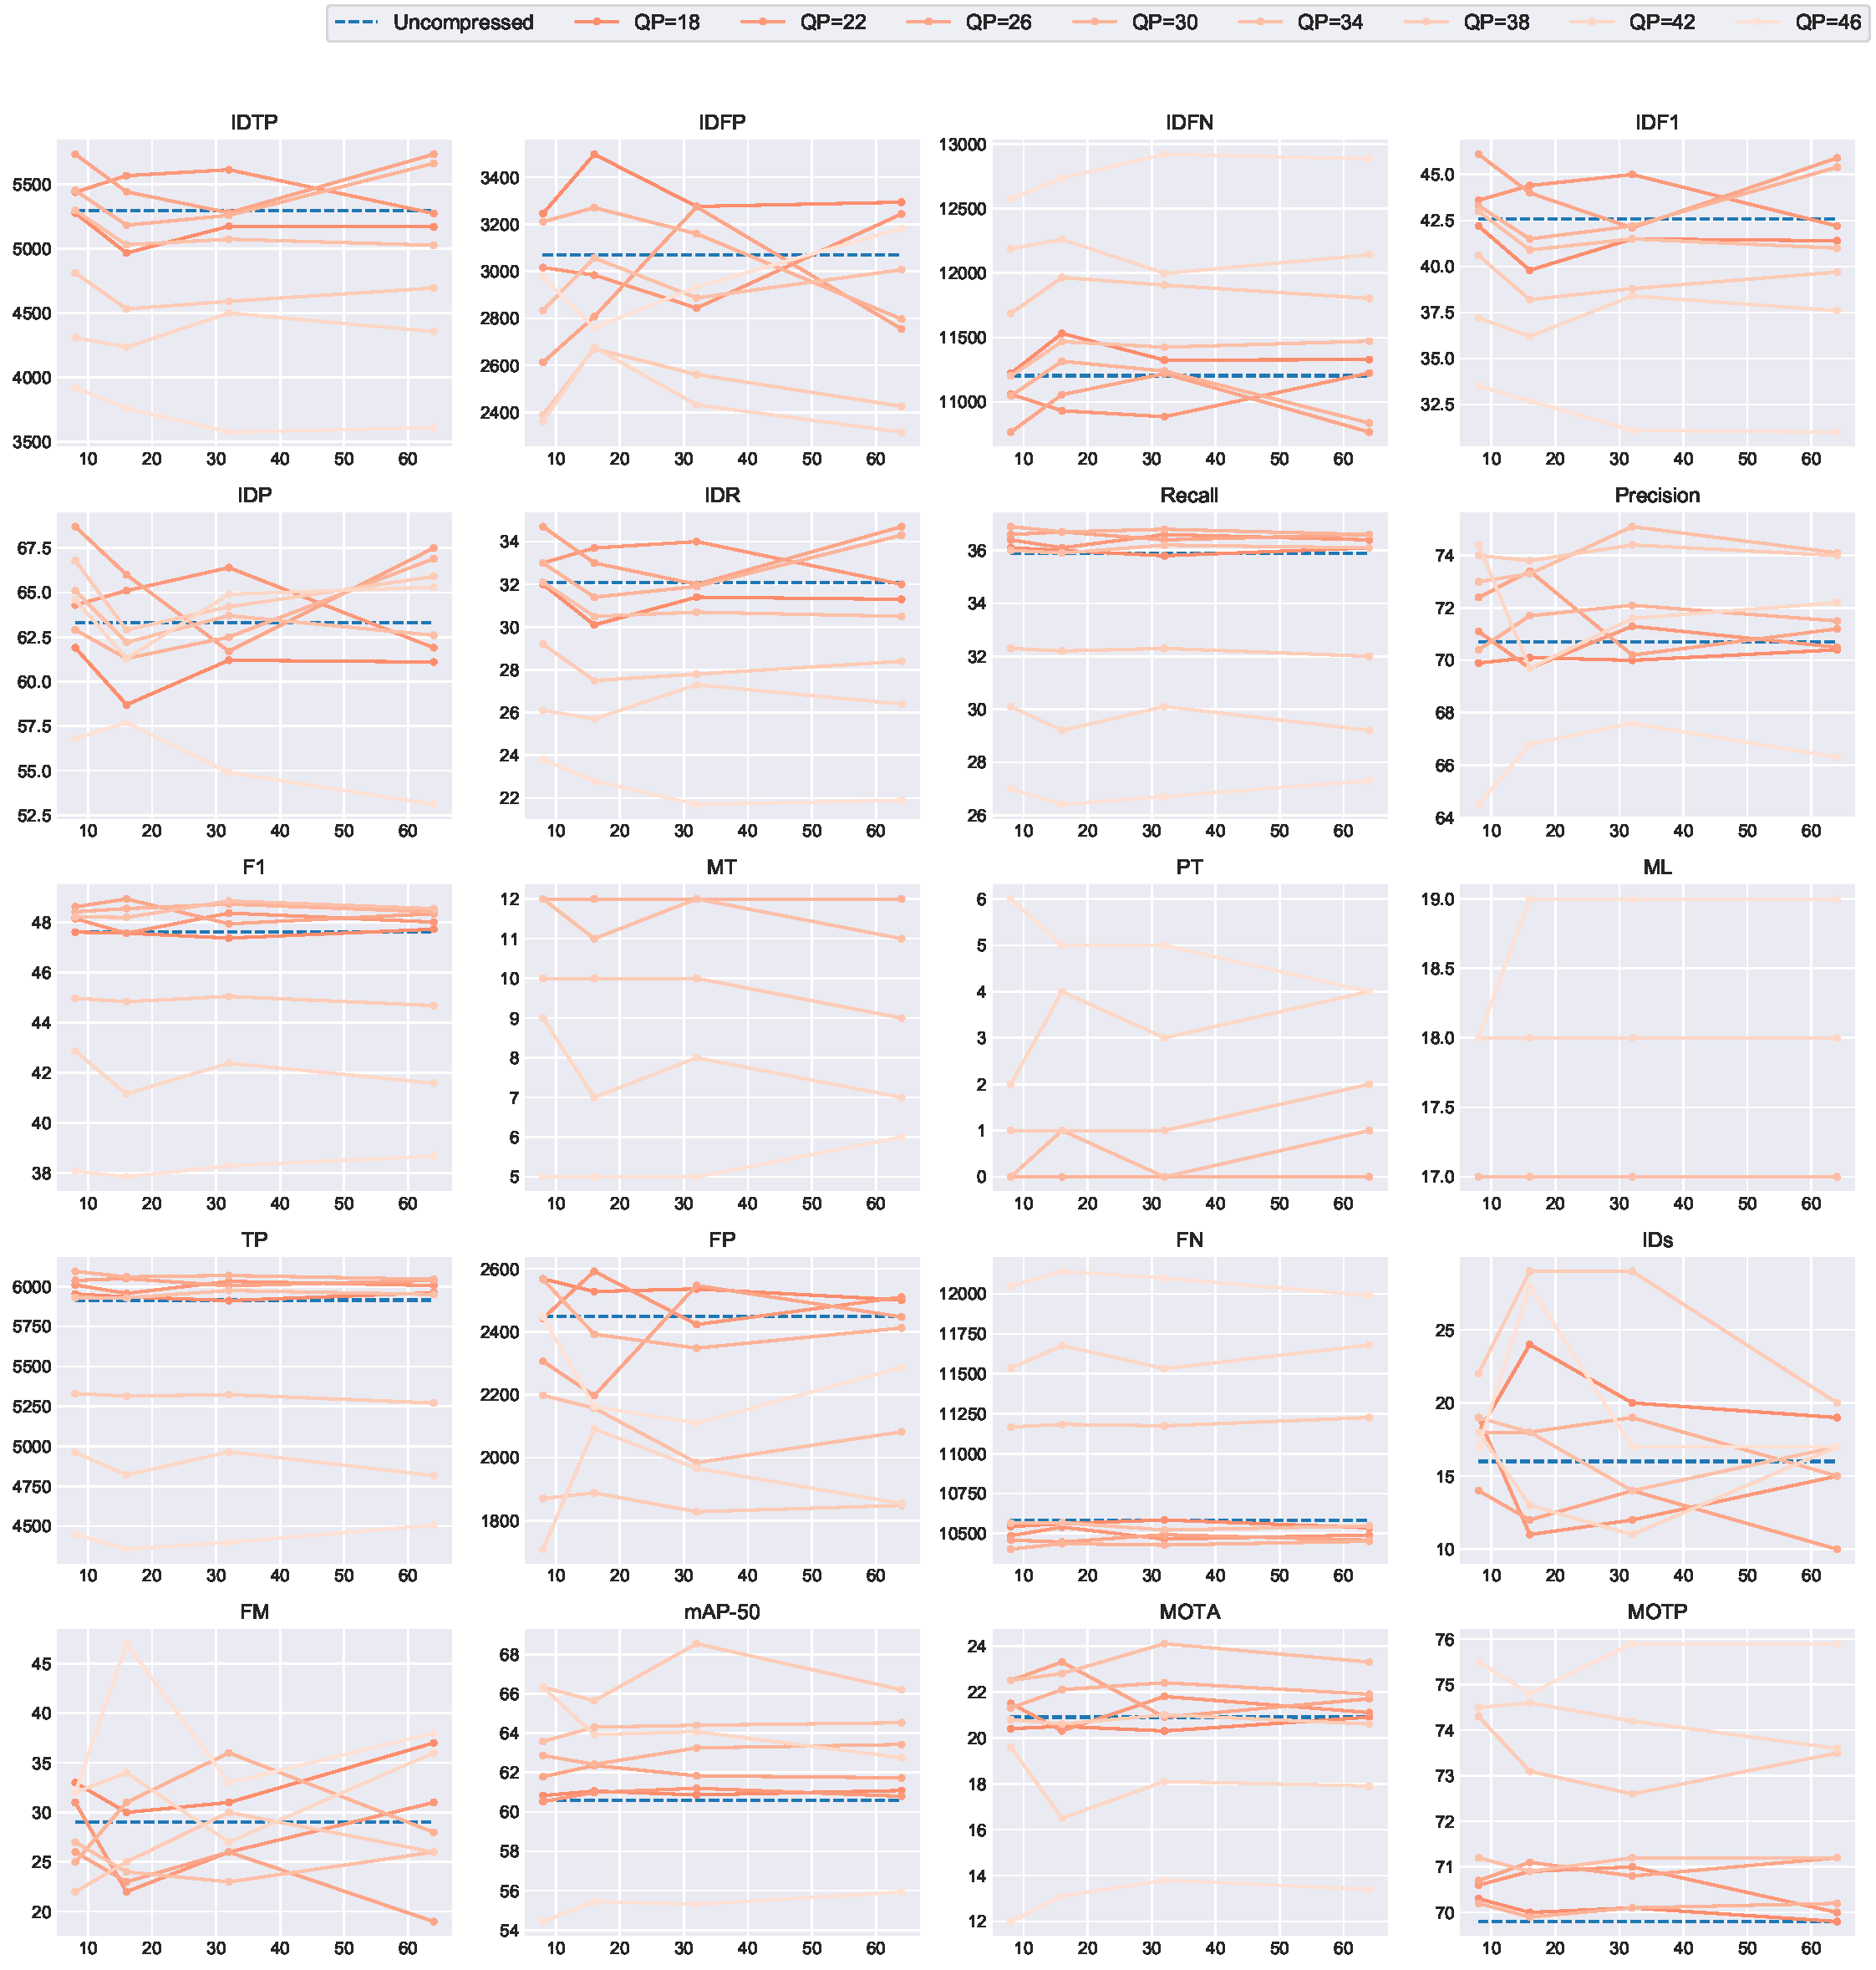
\includegraphics[width=1.0\linewidth]{img/appendix/FourPeople_all_multiplots_msr.pdf}
\caption[Result of all object classes in Class E FourPeople with Horizontal Axis of MSR]{}
\label{fig:FourPeople_all_msr}
\end{figure}



% table
\begin{table}
\centering
\caption{Result of all object classes in Class E FourPeople}


% table for uncompressed
\begin{subtable}[t]{\linewidth}
\centering
\vspace{0pt}
\resizebox{1.0\linewidth}{!}{
\begin{tabular}{llrrrrrrrrrrrrrrrrrrrr}
\toprule
          QP &          MSR &    IDTP &    IDFP &     IDFN &  IDF1 &   IDP &   IDR &  Recall &  Precision &    F1 &  GT &  MT &  PT &  ML &   TP &   FP &    FN &  IDs &  FM &  MOTA &  MOTP \\
\midrule
Uncompressed & Uncompressed & 5293.00 & 3070.00 & 11204.00 & 42.60 & 63.30 & 32.10 &   35.90 &      70.70 & 47.62 &  29 &  12 &   0 &  17 & 5915 & 2448 & 10582 &   16 &  29 & 20.90 & 69.80 \\
\bottomrule
\end{tabular}

}
\caption{Uncompressed Sequence}
\end{subtable}


% table for msr=8
\begin{subtable}[t]{\linewidth}
\centering
\resizebox{1.0\linewidth}{!}{
\begin{tabular}{rrrrrrrrrrrrrrrrrrrrrr}
\toprule
 QP &  MSR &    IDTP &    IDFP &     IDFN &  IDF1 &   IDP &   IDR &  Recall &  Precision &    F1 &  GT &  MT &  PT &  ML &   TP &   FP &    FN &  IDs &  FM &  MOTA &  MOTP \\
\midrule
 18 &    8 & 5275.00 & 3246.00 & 11222.00 & 42.20 & 61.90 & 32.00 &   36.10 &      69.90 & 47.61 &  29 &  12 &   0 &  17 & 5953 & 2568 & 10544 &   18 &  33 & 20.40 & 70.30 \\
 22 &    8 & 5437.00 & 3016.00 & 11060.00 & 43.60 & 64.30 & 33.00 &   36.40 &      71.10 & 48.15 &  29 &  12 &   0 &  17 & 6010 & 2443 & 10487 &   19 &  31 & 21.50 & 70.60 \\
 26 &    8 & 5731.00 & 2613.00 & 10766.00 & 46.10 & 68.70 & 34.70 &   36.60 &      72.40 & 48.62 &  29 &  12 &   0 &  17 & 6038 & 2306 & 10459 &   14 &  26 & 22.50 & 70.70 \\
 30 &    8 & 5450.00 & 3211.00 & 11047.00 & 43.30 & 62.90 & 33.00 &   36.90 &      70.40 & 48.42 &  29 &  12 &   0 &  17 & 6095 & 2566 & 10402 &   18 &  25 & 21.30 & 70.20 \\
 34 &    8 & 5295.00 & 2834.00 & 11202.00 & 43.00 & 65.10 & 32.10 &   36.00 &      73.00 & 48.22 &  29 &  12 &   0 &  17 & 5931 & 2198 & 10566 &   19 &  27 & 22.50 & 71.20 \\
 38 &    8 & 4810.00 & 2390.00 & 11687.00 & 40.60 & 66.80 & 29.20 &   32.30 &      74.00 & 44.97 &  29 &  10 &   1 &  18 & 5330 & 1870 & 11167 &   22 &  22 & 20.80 & 74.30 \\
 42 &    8 & 4309.00 & 2362.00 & 12188.00 & 37.20 & 64.60 & 26.10 &   30.10 &      74.40 & 42.86 &  29 &   9 &   2 &  18 & 4962 & 1709 & 11535 &   18 &  32 & 19.60 & 74.50 \\
 46 &    8 & 3920.00 & 2977.00 & 12577.00 & 33.50 & 56.80 & 23.80 &   27.00 &      64.50 & 38.07 &  29 &   5 &   6 &  18 & 4450 & 2447 & 12047 &   17 &  32 & 12.00 & 75.50 \\
\bottomrule
\end{tabular}

}
\caption{MSR = 8}
\end{subtable}



% table for msr=16
\begin{subtable}[t]{\linewidth}
\centering
\resizebox{1.0\linewidth}{!}{
\begin{tabular}{rrrrrrrrrrrrrrrrrrrrrr}
\toprule
 QP &  MSR &    IDTP &    IDFP &     IDFN &  IDF1 &   IDP &   IDR &  Recall &  Precision &    F1 &  GT &  MT &  PT &  ML &   TP &   FP &    FN &  IDs &  FM &  MOTA &  MOTP \\
\midrule
 18 &   16 & 4965.00 & 3498.00 & 11532.00 & 39.80 & 58.70 & 30.10 &   36.00 &      70.10 & 47.57 &  29 &  12 &   0 &  17 & 5935 & 2528 & 10562 &   24 &  30 & 20.50 & 70.00 \\
 22 &   16 & 5565.00 & 2984.00 & 10932.00 & 44.40 & 65.10 & 33.70 &   36.10 &      69.70 & 47.56 &  29 &  12 &   0 &  17 & 5957 & 2592 & 10540 &   11 &  22 & 20.30 & 70.90 \\
 26 &   16 & 5440.00 & 2807.00 & 11057.00 & 44.00 & 66.00 & 33.00 &   36.70 &      73.40 & 48.93 &  29 &  12 &   0 &  17 & 6050 & 2197 & 10447 &   12 &  23 & 23.30 & 71.10 \\
 30 &   16 & 5181.00 & 3271.00 & 11316.00 & 41.50 & 61.30 & 31.40 &   36.70 &      71.70 & 48.55 &  29 &  12 &   0 &  17 & 6060 & 2392 & 10437 &   18 &  31 & 22.10 & 69.90 \\
 34 &   16 & 5029.00 & 3057.00 & 11468.00 & 40.90 & 62.20 & 30.50 &   35.90 &      73.30 & 48.20 &  29 &  11 &   1 &  17 & 5929 & 2157 & 10568 &   18 &  24 & 22.80 & 70.90 \\
 38 &   16 & 4531.00 & 2671.00 & 11966.00 & 38.20 & 62.90 & 27.50 &   32.20 &      73.80 & 44.84 &  29 &  10 &   1 &  18 & 5314 & 1888 & 11183 &   29 &  25 & 20.60 & 73.10 \\
 42 &   16 & 4235.00 & 2677.00 & 12262.00 & 36.20 & 61.30 & 25.70 &   29.20 &      69.70 & 41.16 &  29 &   7 &   4 &  18 & 4821 & 2091 & 11676 &   13 &  34 & 16.50 & 74.60 \\
 46 &   16 & 3759.00 & 2759.00 & 12738.00 & 32.70 & 57.70 & 22.80 &   26.40 &      66.80 & 37.84 &  29 &   5 &   5 &  19 & 4356 & 2162 & 12141 &   28 &  47 & 13.10 & 74.80 \\
\bottomrule
\end{tabular}

}
\caption{MSR = 16}
\end{subtable}


% table for msr=32
\begin{subtable}[t]{\linewidth}
\centering
\resizebox{1.0\linewidth}{!}{
\begin{tabular}{rrrrrrrrrrrrrrrrrrrrrr}
\toprule
 QP &  MSR &    IDTP &    IDFP &     IDFN &  IDF1 &   IDP &   IDR &  Recall &  Precision &    F1 &  GT &  MT &  PT &  ML &   TP &   FP &    FN &  IDs &  FM &  MOTA &  MOTP \\
\midrule
 18 &   32 & 5172.00 & 3276.00 & 11325.00 & 41.50 & 61.20 & 31.40 &   35.80 &      70.00 & 47.37 &  29 &  12 &   0 &  17 & 5912 & 2536 & 10585 &   20 &  31 & 20.30 & 70.10 \\
 22 &   32 & 5611.00 & 2844.00 & 10886.00 & 45.00 & 66.40 & 34.00 &   36.60 &      71.30 & 48.37 &  29 &  12 &   0 &  17 & 6032 & 2423 & 10465 &   12 &  26 & 21.80 & 71.00 \\
 26 &   32 & 5277.00 & 3274.00 & 11220.00 & 42.10 & 61.70 & 32.00 &   36.40 &      70.20 & 47.94 &  29 &  12 &   0 &  17 & 6004 & 2547 & 10493 &   14 &  26 & 20.90 & 70.80 \\
 30 &   32 & 5257.00 & 3160.00 & 11240.00 & 42.20 & 62.50 & 31.90 &   36.80 &      72.10 & 48.73 &  29 &  12 &   0 &  17 & 6069 & 2348 & 10428 &   19 &  36 & 22.40 & 70.10 \\
 34 &   32 & 5072.00 & 2887.00 & 11425.00 & 41.50 & 63.70 & 30.70 &   36.20 &      75.10 & 48.85 &  29 &  12 &   0 &  17 & 5975 & 1984 & 10522 &   14 &  23 & 24.10 & 71.20 \\
 38 &   32 & 4590.00 & 2561.00 & 11907.00 & 38.80 & 64.20 & 27.80 &   32.30 &      74.40 & 45.04 &  29 &  10 &   1 &  18 & 5323 & 1828 & 11174 &   29 &  30 & 21.00 & 72.60 \\
 42 &   32 & 4499.00 & 2432.00 & 11998.00 & 38.40 & 64.90 & 27.30 &   30.10 &      71.60 & 42.38 &  29 &   8 &   3 &  18 & 4965 & 1966 & 11532 &   11 &  27 & 18.10 & 74.20 \\
 46 &   32 & 3575.00 & 2934.00 & 12922.00 & 31.10 & 54.90 & 21.70 &   26.70 &      67.60 & 38.28 &  29 &   5 &   5 &  19 & 4399 & 2110 & 12098 &   17 &  33 & 13.80 & 75.90 \\
\bottomrule
\end{tabular}

}
\caption{MSR = 32}
\end{subtable}


% table for msr=64
\begin{subtable}[t]{\linewidth}
\centering
\resizebox{1.0\linewidth}{!}{
\begin{tabular}{rrrrrrrrrrrrrrrrrrrrrr}
\toprule
 QP &  MSR &    IDTP &    IDFP &     IDFN &  IDF1 &   IDP &   IDR &  Recall &  Precision &    F1 &  GT &  MT &  PT &  ML &   TP &   FP &    FN &  IDs &  FM &  MOTA &  MOTP \\
\midrule
 18 &   64 & 5168.00 & 3294.00 & 11329.00 & 41.40 & 61.10 & 31.30 &   36.10 &      70.40 & 47.73 &  29 &  12 &   0 &  17 & 5961 & 2501 & 10536 &   19 &  37 & 20.90 & 69.80 \\
 22 &   64 & 5272.00 & 3244.00 & 11225.00 & 42.20 & 61.90 & 32.00 &   36.40 &      70.50 & 48.01 &  29 &  12 &   0 &  17 & 6006 & 2510 & 10491 &   15 &  31 & 21.10 & 70.00 \\
 26 &   64 & 5731.00 & 2755.00 & 10766.00 & 45.90 & 67.50 & 34.70 &   36.60 &      71.20 & 48.35 &  29 &  12 &   0 &  17 & 6039 & 2447 & 10458 &   10 &  19 & 21.70 & 71.20 \\
 30 &   64 & 5660.00 & 2797.00 & 10837.00 & 45.40 & 66.90 & 34.30 &   36.60 &      71.50 & 48.42 &  29 &  12 &   0 &  17 & 6045 & 2412 & 10452 &   15 &  28 & 21.90 & 70.20 \\
 34 &   64 & 5025.00 & 3007.00 & 11472.00 & 41.00 & 62.60 & 30.50 &   36.10 &      74.10 & 48.55 &  29 &  11 &   1 &  17 & 5950 & 2082 & 10547 &   17 &  26 & 23.30 & 71.20 \\
 38 &   64 & 4693.00 & 2426.00 & 11804.00 & 39.70 & 65.90 & 28.40 &   32.00 &      74.00 & 44.68 &  29 &   9 &   2 &  18 & 5271 & 1848 & 11226 &   20 &  26 & 20.60 & 73.50 \\
 42 &   64 & 4355.00 & 2316.00 & 12142.00 & 37.60 & 65.30 & 26.40 &   29.20 &      72.20 & 41.58 &  29 &   7 &   4 &  18 & 4817 & 1854 & 11680 &   17 &  36 & 17.90 & 73.60 \\
 46 &   64 & 3610.00 & 3183.00 & 12887.00 & 31.00 & 53.10 & 21.90 &   27.30 &      66.30 & 38.68 &  29 &   6 &   4 &  19 & 4507 & 2286 & 11990 &   17 &  38 & 13.40 & 75.90 \\
\bottomrule
\end{tabular}

}
\caption{MSR = 64}
\end{subtable}


\label{tab:FourPeople_all}
\end{table}




\begin{table}[!htbp]
\centering
\caption{Multiple Linear Regression Analysis Result for Class E FourPeople}
\resizebox{1.0\linewidth}{!}{
\begin{tabular}{lrrrrrrrrrrrrrrrrrrr}
\toprule
{} &    IDTP &    IDFP &    IDFN &  IDF1 &   IDP &   IDR &  Recall &  Precision &    F1 &    MT &    PT &    ML &      TP &      FP &      FN &   IDs &    FM &  MOTA &  MOTP \\
\midrule
coefficient(Intercept) & 6632.52 & 3556.59 & 9864.48 & 50.72 & 66.13 & 40.20 &   44.44 &      72.65 & 55.99 & 17.48 & -4.21 & 15.73 & 7331.64 & 2857.46 & 9165.36 & 14.64 & 22.29 & 27.02 & 66.14 \\
coefficient(QP)        &  -53.12 &  -20.50 &   53.12 & -0.32 & -0.10 & -0.32 &   -0.33 &      -0.05 & -0.32 & -0.22 &  0.17 &  0.05 &  -54.75 &  -18.86 &   54.75 &  0.13 &  0.20 & -0.22 &  0.19 \\
coefficient(MSR)       &    1.90 &   -0.82 &   -1.90 &  0.02 &  0.02 &  0.01 &   -0.00 &      -0.01 & -0.00 &  0.00 &  0.01 & -0.01 &    0.01 &    1.06 &   -0.01 & -0.01 &  0.05 & -0.01 & -0.01 \\
coefficient(QP*MSR)    &   -0.07 &    0.02 &    0.07 & -0.00 & -0.00 & -0.00 &   -0.00 &       0.00 &  0.00 & -0.00 & -0.00 &  0.00 &   -0.00 &   -0.04 &    0.00 & -0.00 & -0.00 &  0.00 &  0.00 \\
p-value(Intercept)     &    0.00 &    0.00 &    0.00 &  0.00 &  0.00 &  0.00 &    0.00 &       0.00 &  0.00 &  0.00 &  0.00 &  0.00 &    0.00 &    0.00 &    0.00 &  0.01 &  0.00 &  0.00 &  0.00 \\
p-value(QP)            &    0.00 &    0.03 &    0.00 &  0.00 &  0.40 &  0.00 &    0.00 &       0.60 &  0.00 &  0.00 &  0.00 &  0.00 &    0.00 &    0.01 &    0.00 &  0.42 &  0.32 &  0.02 &  0.00 \\
p-value(MSR)           &    0.86 &    0.92 &    0.86 &  0.85 &  0.86 &  0.86 &    0.99 &       0.88 &  0.97 &  0.99 &  0.86 &  0.58 &    1.00 &    0.86 &    1.00 &  0.92 &  0.79 &  0.93 &  0.73 \\
p-value(QP*MSR)        &    0.83 &    0.92 &    0.83 &  0.82 &  0.84 &  0.83 &    1.00 &       0.85 &  0.97 &  0.90 &  0.92 &  0.47 &    0.99 &    0.81 &    0.99 &  0.84 &  0.89 &  0.91 &  0.79 \\
\bottomrule
\end{tabular}

}
\label{tab:FourPeople_all_reg}
\end{table}



\newpage

\section{Class E Johnny}
\label{sec:appendix/Johnny_all}


% visualization figure
\begin{figure}[!htbp]
\centering
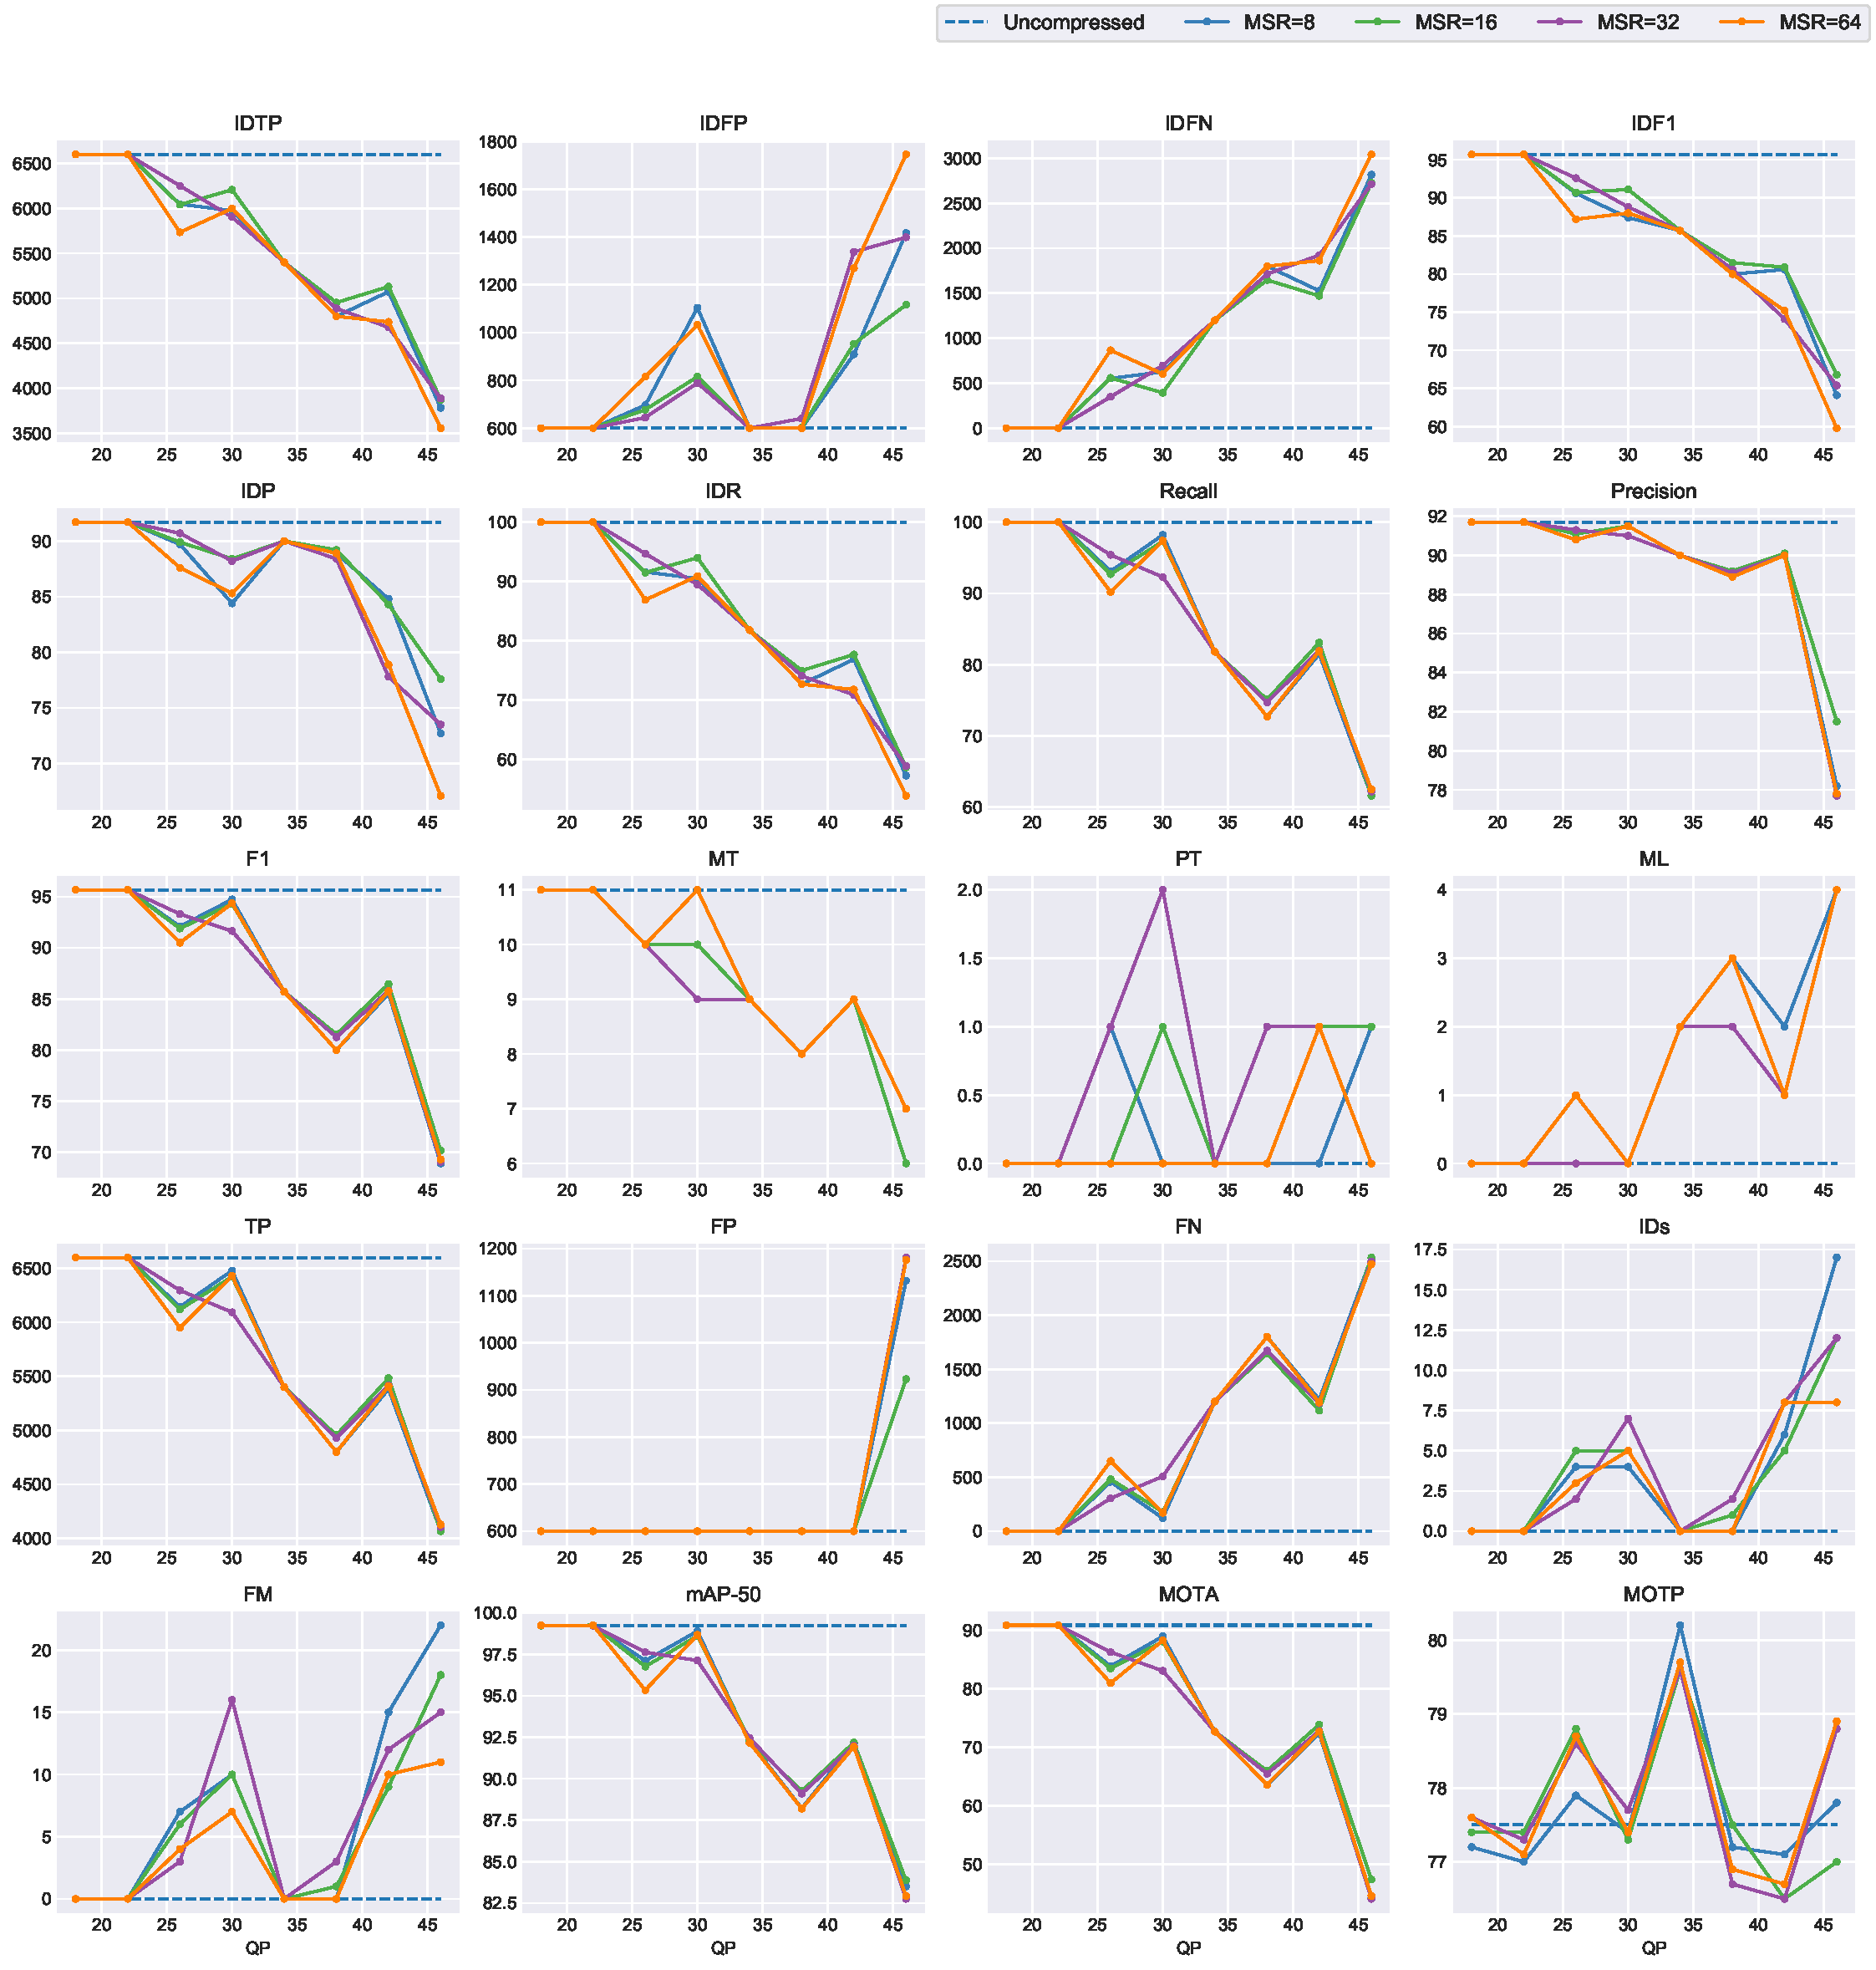
\includegraphics[width=1.0\linewidth]{img/appendix/Johnny_all_multiplots_qp.pdf}
\caption[Visualization of performance results in Class E Johnny at different QP]
{Visualization of performance results in Class E Johnny at different QP.}
\label{fig:Johnny_all_qp}
\end{figure}

\begin{figure}[!htbp]
\centering
\includegraphics[width=1.0\linewidth]{img/appendix/Johnny_all_multiplots_msr.pdf}
\caption[Visualization of performance results in Class E Johnny at different MSR]
{Visualization of performance results in Class E Johnny at different MSR.}
\label{fig:Johnny_all_msr}
\end{figure}



% table
\begin{table}
\centering
\caption[Performance results in Class E Johnny]
{Performance results in Class E Johnny.}


% table for uncompressed
\begin{subtable}[t]{\linewidth}
\centering
\vspace{0pt}
\resizebox{1.0\linewidth}{!}{
\begin{tabular}{llrrrrrrrrrrrrrrrrrrrr}
\toprule
          QP &          MSR &    IDTP &   IDFP &  IDFN &  IDF1 &   IDP &    IDR &  Recall &  Precision &    F1 &  GT &  MT &  PT &  ML &   TP &  FP &  FN &  IDs &  FM &  MOTA &  MOTP \\
\midrule
Uncompressed & Uncompressed & 6600.00 & 600.00 &  0.00 & 95.70 & 91.70 & 100.00 &  100.00 &      91.70 & 95.67 &  11 &  11 &   0 &   0 & 6600 & 600 &   0 &    0 &   0 & 90.90 & 77.50 \\
\bottomrule
\end{tabular}

}
\caption{Uncompressed Sequence}
\end{subtable}


% table for msr=8
\begin{subtable}[t]{\linewidth}
\centering
\resizebox{1.0\linewidth}{!}{
\begin{tabular}{rrrrrrrrrrrrrrrrrrrrrr}
\toprule
 QP &  MSR &    IDTP &    IDFP &    IDFN &  IDF1 &   IDP &    IDR &  Recall &  Precision &    F1 &  GT &  MT &  PT &  ML &   TP &   FP &   FN &  IDs &  FM &  MOTA &  MOTP \\
\midrule
 18 &    8 & 6600.00 &  600.00 &    0.00 & 95.70 & 91.70 & 100.00 &  100.00 &      91.70 & 95.67 &  11 &  11 &   0 &   0 & 6600 &  600 &    0 &    0 &   0 & 90.90 & 77.20 \\
 22 &    8 & 6600.00 &  600.00 &    0.00 & 95.70 & 91.70 & 100.00 &  100.00 &      91.70 & 95.67 &  11 &  11 &   0 &   0 & 6600 &  600 &    0 &    0 &   0 & 90.90 & 77.00 \\
 26 &    8 & 6047.00 &  696.00 &  553.00 & 90.60 & 89.70 &  91.60 &   93.10 &      91.10 & 92.09 &  11 &  10 &   1 &   0 & 6143 &  600 &  457 &    4 &   7 & 83.90 & 77.90 \\
 30 &    8 & 5975.00 & 1104.00 &  625.00 & 87.40 & 84.40 &  90.50 &   98.20 &      91.50 & 94.73 &  11 &  11 &   0 &   0 & 6479 &  600 &  121 &    4 &  10 & 89.00 & 77.40 \\
 34 &    8 & 5400.00 &  600.00 & 1200.00 & 85.70 & 90.00 &  81.80 &   81.80 &      90.00 & 85.70 &  11 &   9 &   0 &   2 & 5400 &  600 & 1200 &    0 &   0 & 72.70 & 80.20 \\
 38 &    8 & 4800.00 &  600.00 & 1800.00 & 80.00 & 88.90 &  72.70 &   72.70 &      88.90 & 79.99 &  11 &   8 &   0 &   3 & 4800 &  600 & 1800 &    0 &   0 & 63.60 & 77.20 \\
 42 &    8 & 5073.00 &  909.00 & 1527.00 & 80.60 & 84.80 &  76.90 &   81.50 &      90.00 & 85.54 &  11 &   9 &   0 &   2 & 5382 &  600 & 1218 &    6 &  15 & 72.40 & 77.10 \\
 46 &    8 & 3782.00 & 1417.00 & 2818.00 & 64.10 & 72.70 &  57.30 &   61.60 &      78.20 & 68.91 &  11 &   6 &   1 &   4 & 4067 & 1132 & 2533 &   17 &  22 & 44.20 & 77.80 \\
\bottomrule
\end{tabular}

}
\caption{MSR = 8}
\end{subtable}



% table for msr=16
\begin{subtable}[t]{\linewidth}
\centering
\resizebox{1.0\linewidth}{!}{
\begin{tabular}{rrrrrrrrrrrrrrrrrrrrrr}
\toprule
 QP &  MSR &    IDTP &    IDFP &    IDFN &  IDF1 &   IDP &    IDR &  Recall &  Precision &    F1 &  GT &  MT &  PT &  ML &   TP &  FP &   FN &  IDs &  FM &  MOTA &  MOTP \\
\midrule
 18 &   16 & 6600.00 &  600.00 &    0.00 & 95.70 & 91.70 & 100.00 &  100.00 &      91.70 & 95.67 &  11 &  11 &   0 &   0 & 6600 & 600 &    0 &    0 &   0 & 90.90 & 77.40 \\
 22 &   16 & 6600.00 &  600.00 &    0.00 & 95.70 & 91.70 & 100.00 &  100.00 &      91.70 & 95.67 &  11 &  11 &   0 &   0 & 6600 & 600 &    0 &    0 &   0 & 90.90 & 77.40 \\
 26 &   16 & 6042.00 &  677.00 &  558.00 & 90.70 & 89.90 &  91.50 &   92.70 &      91.10 & 91.89 &  11 &  10 &   0 &   1 & 6119 & 600 &  481 &    5 &   6 & 83.50 & 78.80 \\
 30 &   16 & 6207.00 &  815.00 &  393.00 & 91.10 & 88.40 &  94.00 &   97.30 &      91.50 & 94.31 &  11 &  10 &   1 &   0 & 6422 & 600 &  178 &    5 &  10 & 88.10 & 77.30 \\
 34 &   16 & 5400.00 &  600.00 & 1200.00 & 85.70 & 90.00 &  81.80 &   81.80 &      90.00 & 85.70 &  11 &   9 &   0 &   2 & 5400 & 600 & 1200 &    0 &   0 & 72.70 & 79.60 \\
 38 &   16 & 4953.00 &  602.00 & 1647.00 & 81.50 & 89.20 &  75.00 &   75.10 &      89.20 & 81.54 &  11 &   8 &   1 &   2 & 4955 & 600 & 1645 &    1 &   1 & 66.00 & 77.50 \\
 42 &   16 & 5130.00 &  953.00 & 1470.00 & 80.90 & 84.30 &  77.70 &   83.10 &      90.10 & 86.46 &  11 &   9 &   1 &   1 & 5483 & 600 & 1117 &    5 &   9 & 73.90 & 76.50 \\
 46 &   16 & 3873.00 & 1116.00 & 2727.00 & 66.80 & 77.60 &  58.70 &   61.60 &      81.50 & 70.17 &  11 &   6 &   1 &   4 & 4066 & 923 & 2534 &   12 &  18 & 47.40 & 77.00 \\
\bottomrule
\end{tabular}

}
\caption{MSR = 16}
\end{subtable}


% table for msr=32
\begin{subtable}[t]{\linewidth}
\centering
\resizebox{1.0\linewidth}{!}{
\begin{tabular}{rrrrrrrrrrrrrrrrrrrrrr}
\toprule
 QP &  MSR &    IDTP &    IDFP &    IDFN &  IDF1 &   IDP &    IDR &  Recall &  Precision &    F1 &  GT &  MT &  PT &  ML &   TP &   FP &   FN &  IDs &  FM &  MOTA &  MOTP \\
\midrule
 18 &   32 & 6600.00 &  600.00 &    0.00 & 95.70 & 91.70 & 100.00 &  100.00 &      91.70 & 95.67 &  11 &  11 &   0 &   0 & 6600 &  600 &    0 &    0 &   0 & 90.90 & 77.60 \\
 22 &   32 & 6600.00 &  600.00 &    0.00 & 95.70 & 91.70 & 100.00 &  100.00 &      91.70 & 95.67 &  11 &  11 &   0 &   0 & 6600 &  600 &    0 &    0 &   0 & 90.90 & 77.30 \\
 26 &   32 & 6252.00 &  644.00 &  348.00 & 92.60 & 90.70 &  94.70 &   95.40 &      91.30 & 93.30 &  11 &  10 &   1 &   0 & 6296 &  600 &  304 &    2 &   3 & 86.30 & 78.60 \\
 30 &   32 & 5904.00 &  789.00 &  696.00 & 88.80 & 88.20 &  89.50 &   92.30 &      91.00 & 91.65 &  11 &   9 &   2 &   0 & 6093 &  600 &  507 &    7 &  16 & 83.10 & 77.70 \\
 34 &   32 & 5400.00 &  600.00 & 1200.00 & 85.70 & 90.00 &  81.80 &   81.80 &      90.00 & 85.70 &  11 &   9 &   0 &   2 & 5400 &  600 & 1200 &    0 &   0 & 72.70 & 79.60 \\
 38 &   32 & 4888.00 &  640.00 & 1712.00 & 80.60 & 88.40 &  74.10 &   74.70 &      89.10 & 81.27 &  11 &   8 &   1 &   2 & 4928 &  600 & 1672 &    2 &   3 & 65.50 & 76.70 \\
 42 &   32 & 4677.00 & 1338.00 & 1923.00 & 74.10 & 77.80 &  70.90 &   82.00 &      90.00 & 85.81 &  11 &   9 &   1 &   1 & 5415 &  600 & 1185 &    8 &  12 & 72.80 & 76.50 \\
 46 &   32 & 3886.00 & 1399.00 & 2714.00 & 65.40 & 73.50 &  58.90 &   62.20 &      77.70 & 69.09 &  11 &   7 &   0 &   4 & 4104 & 1181 & 2496 &   12 &  15 & 44.10 & 78.80 \\
\bottomrule
\end{tabular}

}
\caption{MSR = 32}
\end{subtable}


% table for msr=64
\begin{subtable}[t]{\linewidth}
\centering
\resizebox{1.0\linewidth}{!}{
\begin{tabular}{rrrrrrrrrrrrrrrrrrrrrr}
\toprule
 QP &  MSR &    IDTP &    IDFP &    IDFN &  IDF1 &   IDP &    IDR &  Recall &  Precision &    F1 &  GT &  MT &  PT &  ML &   TP &   FP &   FN &  IDs &  FM &  MOTA &  MOTP \\
\midrule
 18 &   64 & 6600.00 &  600.00 &    0.00 & 95.70 & 91.70 & 100.00 &  100.00 &      91.70 & 95.67 &  11 &  11 &   0 &   0 & 6600 &  600 &    0 &    0 &   0 & 90.90 & 77.60 \\
 22 &   64 & 6600.00 &  600.00 &    0.00 & 95.70 & 91.70 & 100.00 &  100.00 &      91.70 & 95.67 &  11 &  11 &   0 &   0 & 6600 &  600 &    0 &    0 &   0 & 90.90 & 77.10 \\
 26 &   64 & 5735.00 &  815.00 &  865.00 & 87.20 & 87.60 &  86.90 &   90.20 &      90.80 & 90.50 &  11 &  10 &   0 &   1 & 5950 &  600 &  650 &    3 &   4 & 81.00 & 78.70 \\
 30 &   64 & 5998.00 & 1032.00 &  602.00 & 88.00 & 85.30 &  90.90 &   97.40 &      91.50 & 94.36 &  11 &  11 &   0 &   0 & 6430 &  600 &  170 &    5 &   7 & 88.30 & 77.40 \\
 34 &   64 & 5400.00 &  600.00 & 1200.00 & 85.70 & 90.00 &  81.80 &   81.80 &      90.00 & 85.70 &  11 &   9 &   0 &   2 & 5400 &  600 & 1200 &    0 &   0 & 72.70 & 79.70 \\
 38 &   64 & 4800.00 &  600.00 & 1800.00 & 80.00 & 88.90 &  72.70 &   72.70 &      88.90 & 79.99 &  11 &   8 &   0 &   3 & 4800 &  600 & 1800 &    0 &   0 & 63.60 & 76.90 \\
 42 &   64 & 4738.00 & 1270.00 & 1862.00 & 75.20 & 78.90 &  71.80 &   81.90 &      90.00 & 85.76 &  11 &   9 &   1 &   1 & 5408 &  600 & 1192 &    8 &  10 & 72.70 & 76.70 \\
 46 &   64 & 3557.00 & 1746.00 & 3043.00 & 59.80 & 67.10 &  53.90 &   62.50 &      77.80 & 69.32 &  11 &   7 &   0 &   4 & 4127 & 1176 & 2473 &    8 &  11 & 44.60 & 78.90 \\
\bottomrule
\end{tabular}

}
\caption{MSR = 64}
\end{subtable}


\label{tab:Johnny_all}
\end{table}




\begin{table}[!htbp]
\centering
\caption[Multiple linear regression analysis result for Class E Johnny]
{Multiple linear regression analysis result for Class E Johnny}
\resizebox{1.0\linewidth}{!}{
\begin{tabular}{lrrrrrrrrrrrrrrrrrrr}
\toprule
{} &    IDTP &   IDFP &     IDFN &   IDF1 &    IDP &    IDR &  Recall &  Precision &     F1 &    MT &    PT &    ML &      TP &     FP &       FN &   IDs &     FM &   MOTA &  MOTP \\
\midrule
coefficient(Intercept) & 8524.40 & 266.65 & -1924.40 & 115.63 & 101.01 & 129.13 &  127.64 &      98.84 & 113.77 & 14.27 & -0.30 & -2.97 & 8423.59 & 367.46 & -1823.59 & -7.98 & -11.23 & 122.16 & 77.88 \\
coefficient(QP)        &  -91.49 &  15.30 &    91.49 &  -0.93 &  -0.42 &  -1.39 &   -1.29 &      -0.30 &  -0.82 & -0.16 &  0.02 &  0.13 &  -85.14 &   8.94 &    85.14 &  0.37 &   0.57 &  -1.43 & -0.01 \\
coefficient(MSR)       &    2.64 &  -5.86 &    -2.64 &   0.06 &   0.10 &   0.04 &   -0.03 &       0.02 &  -0.01 & -0.01 &  0.00 &  0.01 &   -1.89 &  -1.33 &     1.89 &  0.05 &   0.08 &  -0.01 & -0.00 \\
coefficient(QP*MSR)    &   -0.16 &   0.25 &     0.16 &  -0.00 &  -0.00 &  -0.00 &    0.00 &      -0.00 &   0.00 &  0.00 & -0.00 & -0.00 &    0.04 &   0.05 &    -0.04 & -0.00 &  -0.00 &  -0.00 &  0.00 \\
p-value(Intercept)     &    0.00 &   0.31 &     0.00 &   0.00 &   0.00 &   0.00 &    0.00 &       0.00 &   0.00 &  0.00 &  0.62 &  0.00 &    0.00 &   0.03 &     0.00 &  0.04 &   0.06 &   0.00 &  0.00 \\
p-value(QP)            &    0.00 &   0.06 &     0.00 &   0.00 &   0.00 &   0.00 &    0.00 &       0.01 &   0.00 &  0.00 &  0.18 &  0.00 &    0.00 &   0.08 &     0.00 &  0.00 &   0.00 &   0.00 &  0.86 \\
p-value(MSR)           &    0.76 &   0.41 &     0.76 &   0.56 &   0.43 &   0.75 &    0.87 &       0.86 &   0.95 &  0.66 &  0.91 &  0.77 &    0.87 &   0.77 &     0.87 &  0.64 &   0.59 &   0.97 &  0.90 \\
p-value(QP*MSR)        &    0.53 &   0.24 &     0.53 &   0.34 &   0.25 &   0.53 &    0.90 &       0.81 &   0.98 &  0.55 &  0.72 &  0.78 &    0.90 &   0.71 &     0.90 &  0.53 &   0.40 &   0.99 &  0.81 \\
\bottomrule
\end{tabular}

}
\label{tab:Johnny_all_reg}
\end{table}



\newpage

\section{Class E KristenAndSara}
\label{sec:appendix/KristenAndSara_all}


% visualization figure
\begin{figure}[!htbp]
\centering
\includegraphics[width=1.0\linewidth]{img/appendix/KristenAndSara_all_multiplots_qp.pdf}
\caption[Visualization of performance results in Class E KristenAndSara at different QP]
{Visualization of performance results in Class E KristenAndSara at different QP.}
\label{fig:KristenAndSara_all_qp}
\end{figure}

\begin{figure}[!htbp]
\centering
\includegraphics[width=1.0\linewidth]{img/appendix/KristenAndSara_all_multiplots_msr.pdf}
\caption[Visualization of performance results in Class E KristenAndSara at different MSR]
{Visualization of performance results in Class E KristenAndSara at different MSR.}
\label{fig:KristenAndSara_all_msr}
\end{figure}



% table
\begin{table}
\centering
\caption[Performance results in Class E KristenAndSara]
{Performance results in Class E KristenAndSara.}


% table for uncompressed
\begin{subtable}[t]{\linewidth}
\centering
\vspace{0pt}
\resizebox{1.0\linewidth}{!}{
\begin{tabular}{llrrrrrrrrrrrrrrrrrrrr}
\toprule
          QP &          MSR &    IDTP &    IDFP &    IDFN &  IDF1 &   IDP &   IDR &  Recall &  Precision &    F1 &  GT &  MT &  PT &  ML &   TP &   FP &   FN &  IDs &  FM &  MOTA &  MOTP \\
\midrule
Uncompressed & Uncompressed & 2474.00 & 1296.00 & 6533.00 & 38.70 & 65.60 & 27.50 &   27.70 &      66.20 & 39.06 &  17 &   4 &   0 &  13 & 2496 & 1274 & 6511 &    2 &   4 & 13.50 & 78.90 \\
\bottomrule
\end{tabular}

}
\caption{Uncompressed Sequence}
\end{subtable}


% table for msr=8
\begin{subtable}[t]{\linewidth}
\centering
\resizebox{1.0\linewidth}{!}{
\begin{tabular}{rrrrrrrrrrrrrrrrrrrrrr}
\toprule
 QP &  MSR &    IDTP &    IDFP &    IDFN &  IDF1 &   IDP &   IDR &  Recall &  Precision &    F1 &  GT &  MT &  PT &  ML &   TP &   FP &   FN &  IDs &  FM &  MOTA &  MOTP \\
\midrule
 18 &    8 & 2481.00 & 1471.00 & 6526.00 & 38.30 & 62.80 & 27.50 &   27.90 &      63.50 & 38.77 &  17 &   4 &   1 &  12 & 2511 & 1441 & 6496 &    3 &   5 & 11.80 & 78.80 \\
 22 &    8 & 2499.00 & 1563.00 & 6508.00 & 38.20 & 61.50 & 27.70 &   28.50 &      63.10 & 39.27 &  17 &   4 &   0 &  13 & 2563 & 1499 & 6444 &    6 &   8 & 11.70 & 78.80 \\
 26 &    8 & 2483.00 & 1455.00 & 6524.00 & 38.40 & 63.10 & 27.60 &   28.40 &      64.90 & 39.51 &  17 &   4 &   0 &  13 & 2556 & 1382 & 6451 &    5 &   7 & 13.00 & 78.90 \\
 30 &    8 & 2710.00 & 1615.00 & 6297.00 & 40.70 & 62.70 & 30.10 &   33.20 &      69.10 & 44.85 &  17 &   4 &   2 &  11 & 2987 & 1338 & 6020 &    6 &   9 & 18.20 & 77.50 \\
 34 &    8 & 2996.00 & 1441.00 & 6011.00 & 44.60 & 67.50 & 33.30 &   33.30 &      67.50 & 44.60 &  17 &   5 &   0 &  12 & 2996 & 1441 & 6011 &    0 &   1 & 17.30 & 77.10 \\
 38 &    8 & 2793.00 & 1322.00 & 6214.00 & 42.60 & 67.90 & 31.00 &   32.70 &      71.60 & 44.90 &  17 &   5 &   0 &  12 & 2947 & 1168 & 6060 &    3 &   5 & 19.70 & 77.20 \\
 42 &    8 & 2786.00 & 1243.00 & 6221.00 & 42.70 & 69.10 & 30.90 &   32.60 &      72.80 & 45.03 &  17 &   5 &   0 &  12 & 2935 & 1094 & 6072 &    2 &  15 & 20.40 & 74.50 \\
 46 &    8 & 1595.00 &  770.00 & 7412.00 & 28.10 & 67.40 & 17.70 &   22.00 &      83.80 & 34.85 &  17 &   3 &   1 &  13 & 1982 &  383 & 7025 &    9 &  15 & 17.70 & 79.60 \\
\bottomrule
\end{tabular}

}
\caption{MSR = 8}
\end{subtable}



% table for msr=16
\begin{subtable}[t]{\linewidth}
\centering
\resizebox{1.0\linewidth}{!}{
\begin{tabular}{rrrrrrrrrrrrrrrrrrrrrr}
\toprule
 QP &  MSR &    IDTP &    IDFP &    IDFN &  IDF1 &   IDP &   IDR &  Recall &  Precision &    F1 &  GT &  MT &  PT &  ML &   TP &   FP &   FN &  IDs &  FM &  MOTA &  MOTP \\
\midrule
 18 &   16 & 2486.00 & 1456.00 & 6521.00 & 38.40 & 63.10 & 27.60 &   27.80 &      63.60 & 38.69 &  17 &   4 &   1 &  12 & 2508 & 1434 & 6499 &    2 &   5 & 11.90 & 78.80 \\
 22 &   16 & 2511.00 & 1517.00 & 6496.00 & 38.50 & 62.30 & 27.90 &   28.40 &      63.60 & 39.27 &  17 &   4 &   0 &  13 & 2560 & 1468 & 6447 &    6 &   9 & 12.10 & 78.80 \\
 26 &   16 & 2492.00 & 1514.00 & 6515.00 & 38.30 & 62.20 & 27.70 &   28.70 &      64.60 & 39.74 &  17 &   4 &   1 &  12 & 2587 & 1419 & 6420 &    4 &   5 & 12.90 & 79.00 \\
 30 &   16 & 2780.00 & 1628.00 & 6227.00 & 41.40 & 63.10 & 30.90 &   32.50 &      66.50 & 43.66 &  17 &   5 &   0 &  12 & 2930 & 1478 & 6077 &    3 &   4 & 16.10 & 78.20 \\
 34 &   16 & 2758.00 & 1663.00 & 6249.00 & 41.10 & 62.40 & 30.60 &   32.80 &      66.80 & 44.00 &  17 &   5 &   0 &  12 & 2953 & 1468 & 6054 &    1 &   2 & 16.50 & 77.20 \\
 38 &   16 & 2823.00 & 1329.00 & 6184.00 & 42.90 & 68.00 & 31.30 &   33.10 &      71.80 & 45.31 &  17 &   5 &   0 &  12 & 2980 & 1172 & 6027 &    2 &   3 & 20.10 & 77.10 \\
 42 &   16 & 2621.00 & 1197.00 & 6386.00 & 40.90 & 68.60 & 29.10 &   31.20 &      73.70 & 43.84 &  17 &   4 &   1 &  12 & 2814 & 1004 & 6193 &    4 &  16 & 20.10 & 75.10 \\
 46 &   16 & 1888.00 &  506.00 & 7119.00 & 33.10 & 78.90 & 21.00 &   22.90 &      86.30 & 36.20 &  17 &   3 &   1 &  13 & 2065 &  329 & 6942 &    5 &  20 & 19.20 & 78.40 \\
\bottomrule
\end{tabular}

}
\caption{MSR = 16}
\end{subtable}


% table for msr=32
\begin{subtable}[t]{\linewidth}
\centering
\resizebox{1.0\linewidth}{!}{
\begin{tabular}{rrrrrrrrrrrrrrrrrrrrrr}
\toprule
 QP &  MSR &    IDTP &    IDFP &    IDFN &  IDF1 &   IDP &   IDR &  Recall &  Precision &    F1 &  GT &  MT &  PT &  ML &   TP &   FP &   FN &  IDs &  FM &  MOTA &  MOTP \\
\midrule
 18 &   32 & 2483.00 & 1470.00 & 6524.00 & 38.30 & 62.80 & 27.60 &   27.90 &      63.50 & 38.77 &  17 &   4 &   0 &  13 & 2511 & 1442 & 6496 &    2 &   4 & 11.80 & 78.90 \\
 22 &   32 & 2506.00 & 1565.00 & 6501.00 & 38.30 & 61.60 & 27.80 &   29.40 &      64.90 & 40.47 &  17 &   4 &   1 &  12 & 2644 & 1427 & 6363 &    9 &  15 & 13.40 & 78.50 \\
 26 &   32 & 2502.00 & 1484.00 & 6505.00 & 38.50 & 62.80 & 27.80 &   28.70 &      64.80 & 39.78 &  17 &   4 &   0 &  13 & 2581 & 1405 & 6426 &    6 &   7 & 13.00 & 78.80 \\
 30 &   32 & 2558.00 & 1805.00 & 6449.00 & 38.30 & 58.60 & 28.40 &   31.90 &      65.80 & 42.97 &  17 &   4 &   1 &  12 & 2872 & 1491 & 6135 &    8 &   9 & 15.20 & 78.80 \\
 34 &   32 & 2774.00 & 1574.00 & 6233.00 & 41.50 & 63.80 & 30.80 &   33.00 &      68.40 & 44.52 &  17 &   5 &   0 &  12 & 2975 & 1373 & 6032 &    1 &   4 & 17.80 & 77.40 \\
 38 &   32 & 2993.00 & 1168.00 & 6014.00 & 45.50 & 71.90 & 33.20 &   33.30 &      72.00 & 45.54 &  17 &   5 &   0 &  12 & 2996 & 1165 & 6011 &    1 &   3 & 20.30 & 77.10 \\
 42 &   32 & 2585.00 & 1153.00 & 6422.00 & 40.60 & 69.20 & 28.70 &   31.10 &      74.90 & 43.95 &  17 &   4 &   1 &  12 & 2798 &  940 & 6209 &    4 &  10 & 20.60 & 75.10 \\
 46 &   32 & 1543.00 &  894.00 & 7464.00 & 27.00 & 63.30 & 17.10 &   21.50 &      79.40 & 33.84 &  17 &   3 &   1 &  13 & 1935 &  502 & 7072 &   15 &  25 & 15.70 & 80.30 \\
\bottomrule
\end{tabular}

}
\caption{MSR = 32}
\end{subtable}


% table for msr=64
\begin{subtable}[t]{\linewidth}
\centering
\resizebox{1.0\linewidth}{!}{
\begin{tabular}{rrrrrrrrrrrrrrrrrrrrrr}
\toprule
 QP &  MSR &    IDTP &    IDFP &    IDFN &  IDF1 &   IDP &   IDR &  Recall &  Precision &    F1 &  GT &  MT &  PT &  ML &   TP &   FP &   FN &  IDs &  FM &  MOTA &  MOTP \\
\midrule
 18 &   64 & 2485.00 & 1522.00 & 6522.00 & 38.20 & 62.00 & 27.60 &   28.00 &      62.90 & 38.75 &  17 &   4 &   0 &  13 & 2522 & 1485 & 6485 &    4 &   5 & 11.50 & 78.80 \\
 22 &   64 & 2528.00 & 1567.00 & 6479.00 & 38.60 & 61.70 & 28.10 &   28.90 &      63.50 & 39.72 &  17 &   4 &   1 &  12 & 2600 & 1495 & 6407 &    6 &  11 & 12.20 & 78.50 \\
 26 &   64 & 2512.00 & 1453.00 & 6495.00 & 38.70 & 63.40 & 27.90 &   29.40 &      66.70 & 40.81 &  17 &   4 &   1 &  12 & 2645 & 1320 & 6362 &    6 &  13 & 14.60 & 78.40 \\
 30 &   64 & 2543.00 & 1726.00 & 6464.00 & 38.30 & 59.60 & 28.20 &   31.00 &      65.40 & 42.06 &  17 &   4 &   1 &  12 & 2790 & 1479 & 6217 &    6 &   9 & 14.50 & 79.20 \\
 34 &   64 & 2756.00 & 1583.00 & 6251.00 & 41.30 & 63.50 & 30.60 &   33.30 &      69.20 & 44.96 &  17 &   5 &   0 &  12 & 3001 & 1338 & 6006 &    1 &   1 & 18.50 & 77.00 \\
 38 &   64 & 2832.00 & 1301.00 & 6175.00 & 43.10 & 68.50 & 31.40 &   33.10 &      72.10 & 45.37 &  17 &   5 &   0 &  12 & 2981 & 1152 & 6026 &    3 &   6 & 20.30 & 77.20 \\
 42 &   64 & 2675.00 & 1210.00 & 6332.00 & 41.50 & 68.90 & 29.70 &   31.50 &      72.90 & 43.99 &  17 &   4 &   1 &  12 & 2833 & 1052 & 6174 &    3 &  17 & 19.70 & 75.10 \\
 46 &   64 & 1483.00 &  780.00 & 7524.00 & 26.30 & 65.50 & 16.50 &   19.90 &      79.20 & 31.81 &  17 &   3 &   0 &  14 & 1792 &  471 & 7215 &   10 &  22 & 14.60 & 80.80 \\
\bottomrule
\end{tabular}

}
\caption{MSR = 64}
\end{subtable}


\label{tab:KristenAndSara_all}
\end{table}




\begin{table}[!htbp]
\centering
\caption[Multiple linear regression analysis result for Class E KristenAndSara]
{Multiple linear regression analysis result for Class E KristenAndSara}
\resizebox{1.0\linewidth}{!}{
\begin{tabular}{lrrrrrrrrrrrrrrrrrrr}
\toprule
{} &    IDTP &    IDFP &    IDFN &  IDF1 &   IDP &   IDR &  Recall &  Precision &    F1 &    MT &    PT &    ML &      TP &      FP &      FN &  IDs &    FM &  MOTA &  MOTP \\
\midrule
coefficient(Intercept) & 2825.44 & 2092.96 & 6181.56 & 41.18 & 54.13 & 31.37 &   30.16 &      48.42 & 39.15 &  4.30 &  0.28 & 12.41 & 2714.85 & 2203.56 & 6292.15 & 2.72 & -2.31 &  5.59 & 80.33 \\
coefficient(QP)        &   -8.51 &  -23.15 &    8.51 & -0.06 &  0.36 & -0.09 &   -0.01 &       0.66 &  0.07 & -0.00 &  0.01 & -0.01 &   -0.86 &  -30.80 &    0.86 & 0.04 &  0.31 &  0.33 & -0.08 \\
coefficient(MSR)       &    2.19 &    0.37 &   -2.19 &  0.03 &  0.04 &  0.02 &    0.03 &       0.06 &  0.05 &  0.00 &  0.01 & -0.01 &    3.12 &   -0.56 &   -3.12 & 0.01 &  0.02 &  0.04 & -0.02 \\
coefficient(QP*MSR)    &   -0.11 &    0.01 &    0.11 & -0.00 & -0.00 & -0.00 &   -0.00 &      -0.00 & -0.00 & -0.00 & -0.00 &  0.00 &   -0.12 &    0.02 &    0.12 & 0.00 &  0.00 & -0.00 &  0.00 \\
p-value(Intercept)     &    0.00 &    0.00 &    0.00 &  0.00 &  0.00 &  0.00 &    0.00 &       0.00 &  0.00 &  0.00 &  0.67 &  0.00 &    0.00 &    0.00 &    0.00 & 0.46 &  0.71 &  0.01 &  0.00 \\
p-value(QP)            &    0.50 &    0.00 &    0.50 &  0.72 &  0.00 &  0.50 &    0.94 &       0.00 &  0.57 &  0.95 &  0.74 &  0.79 &    0.94 &    0.00 &    0.94 & 0.72 &  0.10 &  0.00 &  0.11 \\
p-value(MSR)           &    0.85 &    0.95 &    0.85 &  0.82 &  0.66 &  0.84 &    0.77 &       0.49 &  0.70 &  0.90 &  0.76 &  0.66 &    0.77 &    0.93 &    0.77 & 0.95 &  0.89 &  0.48 &  0.62 \\
p-value(QP*MSR)        &    0.75 &    0.96 &    0.75 &  0.70 &  0.44 &  0.75 &    0.71 &       0.39 &  0.63 &  0.80 &  0.75 &  0.56 &    0.71 &    0.92 &    0.71 & 0.88 &  0.89 &  0.38 &  0.51 \\
\bottomrule
\end{tabular}

}
\label{tab:KristenAndSara_all_reg}
\end{table}










\end{document}
